% Options for packages loaded elsewhere
\PassOptionsToPackage{unicode}{hyperref}
\PassOptionsToPackage{hyphens}{url}
%
\documentclass[
]{book}
\usepackage{amsmath,amssymb}
\usepackage{iftex}
\ifPDFTeX
  \usepackage[T1]{fontenc}
  \usepackage[utf8]{inputenc}
  \usepackage{textcomp} % provide euro and other symbols
\else % if luatex or xetex
  \usepackage{unicode-math} % this also loads fontspec
  \defaultfontfeatures{Scale=MatchLowercase}
  \defaultfontfeatures[\rmfamily]{Ligatures=TeX,Scale=1}
\fi
\usepackage{lmodern}
\ifPDFTeX\else
  % xetex/luatex font selection
\fi
% Use upquote if available, for straight quotes in verbatim environments
\IfFileExists{upquote.sty}{\usepackage{upquote}}{}
\IfFileExists{microtype.sty}{% use microtype if available
  \usepackage[]{microtype}
  \UseMicrotypeSet[protrusion]{basicmath} % disable protrusion for tt fonts
}{}
\makeatletter
\@ifundefined{KOMAClassName}{% if non-KOMA class
  \IfFileExists{parskip.sty}{%
    \usepackage{parskip}
  }{% else
    \setlength{\parindent}{0pt}
    \setlength{\parskip}{6pt plus 2pt minus 1pt}}
}{% if KOMA class
  \KOMAoptions{parskip=half}}
\makeatother
\usepackage{xcolor}
\usepackage[margin=2cm]{geometry}
\usepackage{color}
\usepackage{fancyvrb}
\newcommand{\VerbBar}{|}
\newcommand{\VERB}{\Verb[commandchars=\\\{\}]}
\DefineVerbatimEnvironment{Highlighting}{Verbatim}{commandchars=\\\{\}}
% Add ',fontsize=\small' for more characters per line
\usepackage{framed}
\definecolor{shadecolor}{RGB}{248,248,248}
\newenvironment{Shaded}{\begin{snugshade}}{\end{snugshade}}
\newcommand{\AlertTok}[1]{\textcolor[rgb]{0.94,0.16,0.16}{#1}}
\newcommand{\AnnotationTok}[1]{\textcolor[rgb]{0.56,0.35,0.01}{\textbf{\textit{#1}}}}
\newcommand{\AttributeTok}[1]{\textcolor[rgb]{0.13,0.29,0.53}{#1}}
\newcommand{\BaseNTok}[1]{\textcolor[rgb]{0.00,0.00,0.81}{#1}}
\newcommand{\BuiltInTok}[1]{#1}
\newcommand{\CharTok}[1]{\textcolor[rgb]{0.31,0.60,0.02}{#1}}
\newcommand{\CommentTok}[1]{\textcolor[rgb]{0.56,0.35,0.01}{\textit{#1}}}
\newcommand{\CommentVarTok}[1]{\textcolor[rgb]{0.56,0.35,0.01}{\textbf{\textit{#1}}}}
\newcommand{\ConstantTok}[1]{\textcolor[rgb]{0.56,0.35,0.01}{#1}}
\newcommand{\ControlFlowTok}[1]{\textcolor[rgb]{0.13,0.29,0.53}{\textbf{#1}}}
\newcommand{\DataTypeTok}[1]{\textcolor[rgb]{0.13,0.29,0.53}{#1}}
\newcommand{\DecValTok}[1]{\textcolor[rgb]{0.00,0.00,0.81}{#1}}
\newcommand{\DocumentationTok}[1]{\textcolor[rgb]{0.56,0.35,0.01}{\textbf{\textit{#1}}}}
\newcommand{\ErrorTok}[1]{\textcolor[rgb]{0.64,0.00,0.00}{\textbf{#1}}}
\newcommand{\ExtensionTok}[1]{#1}
\newcommand{\FloatTok}[1]{\textcolor[rgb]{0.00,0.00,0.81}{#1}}
\newcommand{\FunctionTok}[1]{\textcolor[rgb]{0.13,0.29,0.53}{\textbf{#1}}}
\newcommand{\ImportTok}[1]{#1}
\newcommand{\InformationTok}[1]{\textcolor[rgb]{0.56,0.35,0.01}{\textbf{\textit{#1}}}}
\newcommand{\KeywordTok}[1]{\textcolor[rgb]{0.13,0.29,0.53}{\textbf{#1}}}
\newcommand{\NormalTok}[1]{#1}
\newcommand{\OperatorTok}[1]{\textcolor[rgb]{0.81,0.36,0.00}{\textbf{#1}}}
\newcommand{\OtherTok}[1]{\textcolor[rgb]{0.56,0.35,0.01}{#1}}
\newcommand{\PreprocessorTok}[1]{\textcolor[rgb]{0.56,0.35,0.01}{\textit{#1}}}
\newcommand{\RegionMarkerTok}[1]{#1}
\newcommand{\SpecialCharTok}[1]{\textcolor[rgb]{0.81,0.36,0.00}{\textbf{#1}}}
\newcommand{\SpecialStringTok}[1]{\textcolor[rgb]{0.31,0.60,0.02}{#1}}
\newcommand{\StringTok}[1]{\textcolor[rgb]{0.31,0.60,0.02}{#1}}
\newcommand{\VariableTok}[1]{\textcolor[rgb]{0.00,0.00,0.00}{#1}}
\newcommand{\VerbatimStringTok}[1]{\textcolor[rgb]{0.31,0.60,0.02}{#1}}
\newcommand{\WarningTok}[1]{\textcolor[rgb]{0.56,0.35,0.01}{\textbf{\textit{#1}}}}
\usepackage{longtable,booktabs,array}
\usepackage{calc} % for calculating minipage widths
% Correct order of tables after \paragraph or \subparagraph
\usepackage{etoolbox}
\makeatletter
\patchcmd\longtable{\par}{\if@noskipsec\mbox{}\fi\par}{}{}
\makeatother
% Allow footnotes in longtable head/foot
\IfFileExists{footnotehyper.sty}{\usepackage{footnotehyper}}{\usepackage{footnote}}
\makesavenoteenv{longtable}
\usepackage{graphicx}
\makeatletter
\def\maxwidth{\ifdim\Gin@nat@width>\linewidth\linewidth\else\Gin@nat@width\fi}
\def\maxheight{\ifdim\Gin@nat@height>\textheight\textheight\else\Gin@nat@height\fi}
\makeatother
% Scale images if necessary, so that they will not overflow the page
% margins by default, and it is still possible to overwrite the defaults
% using explicit options in \includegraphics[width, height, ...]{}
\setkeys{Gin}{width=\maxwidth,height=\maxheight,keepaspectratio}
% Set default figure placement to htbp
\makeatletter
\def\fps@figure{htbp}
\makeatother
\setlength{\emergencystretch}{3em} % prevent overfull lines
\providecommand{\tightlist}{%
  \setlength{\itemsep}{0pt}\setlength{\parskip}{0pt}}
\setcounter{secnumdepth}{5}
\ifLuaTeX
  \usepackage{selnolig}  % disable illegal ligatures
\fi
\usepackage[]{natbib}
\bibliographystyle{apalike}
\nocite{*}
\IfFileExists{bookmark.sty}{\usepackage{bookmark}}{\usepackage{hyperref}}
\IfFileExists{xurl.sty}{\usepackage{xurl}}{} % add URL line breaks if available
\urlstyle{same}
\hypersetup{
  pdftitle={Supplementary Material for `Lexidate Selection Set Analysis: Varying Selection Schemes To Assess Generalizability Of Evolved Machine Learning Pipelines'},
  pdfauthor={Jose Guadalupe Hernandez, Anil Kumar Saini, Jason H. Moore},
  hidelinks,
  pdfcreator={LaTeX via pandoc}}

\title{Supplementary Material for `Lexidate Selection Set Analysis: Varying Selection Schemes To Assess Generalizability Of Evolved Machine Learning Pipelines'}
\author{Jose Guadalupe Hernandez, Anil Kumar Saini, Jason H. Moore}
\date{2024-11-16}

\begin{document}
\maketitle

{
\setcounter{tocdepth}{1}
\tableofcontents
}
\hypertarget{introduction}{%
\chapter{Introduction}\label{introduction}}

This is not intended as a stand-alone document, but as a companion to our manuscript.

\hypertarget{about-our-supplemental-material}{%
\section{About our supplemental material}\label{about-our-supplemental-material}}

As you may have noticed (unless you're reading a pdf version of this), our supplemental material is hosted using \href{https://pages.github.com/}{GitHub pages}.
We compiled our data analyses and supplemental documentation into this nifty web-accessible book using \href{https://bookdown.org}{bookdown}.

The code used for this supplemental material can be found in \href{https://github.com/jgh9094/lexidate-holdout-analysis}{this GitHub repository}.

Our supplemental material includes the following:

\begin{itemize}
\tightlist
\item
  Helper functions (Section \ref{helper-functions})
\end{itemize}

\hypertarget{contributing-authors}{%
\section{Contributing authors}\label{contributing-authors}}

\begin{itemize}
\tightlist
\item
  \href{https://jgh9094.github.io/}{Jose Guadalupe Hernandez}
\item
  \href{https://theaksaini.github.io/}{Anil Kumar Saini}
\item
  \href{https://jasonhmoore.org/}{Jason H. Moore}
\end{itemize}

\hypertarget{helper-functions}{%
\chapter{Helper functions}\label{helper-functions}}

Here we show the functions being used to generate the supplementary material.
All of the following functions are compsed of R code and are used to generate the figures, tables, and statitics.

\hypertarget{setup}{%
\section{Setup}\label{setup}}

\begin{Shaded}
\begin{Highlighting}[]
\FunctionTok{library}\NormalTok{(ggplot2)}
\FunctionTok{library}\NormalTok{(cowplot)}
\FunctionTok{library}\NormalTok{(dplyr)}
\FunctionTok{library}\NormalTok{(PupillometryR)}


\NormalTok{NAMES }\OtherTok{=} \FunctionTok{c}\NormalTok{(}\StringTok{\textquotesingle{}tournament\textquotesingle{}}\NormalTok{, }\StringTok{\textquotesingle{}lexicase\textquotesingle{}}\NormalTok{)}
\NormalTok{SHAPE }\OtherTok{\textless{}{-}} \FunctionTok{c}\NormalTok{(}\DecValTok{21}\NormalTok{, }\DecValTok{21}\NormalTok{)}
\NormalTok{cb\_palette }\OtherTok{\textless{}{-}} \FunctionTok{c}\NormalTok{(}\StringTok{\textquotesingle{}\#DC1E34\textquotesingle{}}\NormalTok{, }\StringTok{\textquotesingle{}\#004D40\textquotesingle{}}\NormalTok{)}
\NormalTok{data\_dir }\OtherTok{\textless{}{-}} \StringTok{\textquotesingle{}./\textquotesingle{}}
\NormalTok{c\_task\_id\_lists }\OtherTok{\textless{}{-}} \FunctionTok{c}\NormalTok{(}\DecValTok{146818}\NormalTok{,}\DecValTok{359954}\NormalTok{,}\DecValTok{359955}\NormalTok{,}\DecValTok{190146}\NormalTok{,}\DecValTok{168757}\NormalTok{,}\DecValTok{359956}\NormalTok{,}
                        \DecValTok{359958}\NormalTok{,}\DecValTok{359959}\NormalTok{,}\DecValTok{2073}\NormalTok{,}\DecValTok{359960}\NormalTok{,}\DecValTok{168784}\NormalTok{,}\DecValTok{359962}\NormalTok{)}

\NormalTok{p\_theme }\OtherTok{\textless{}{-}} \FunctionTok{theme}\NormalTok{(}
  \AttributeTok{plot.title =} \FunctionTok{element\_text}\NormalTok{(}\AttributeTok{face =} \StringTok{"bold"}\NormalTok{, }\AttributeTok{size =} \DecValTok{17}\NormalTok{, }\AttributeTok{hjust=}\FloatTok{0.5}\NormalTok{),}
  \AttributeTok{panel.border =} \FunctionTok{element\_blank}\NormalTok{(),}
  \AttributeTok{panel.grid.minor =} \FunctionTok{element\_blank}\NormalTok{(),}
  \AttributeTok{legend.title=}\FunctionTok{element\_text}\NormalTok{(}\AttributeTok{size=}\DecValTok{17}\NormalTok{),}
  \AttributeTok{legend.text=}\FunctionTok{element\_text}\NormalTok{(}\AttributeTok{size=}\DecValTok{17}\NormalTok{),}
  \AttributeTok{axis.title =} \FunctionTok{element\_text}\NormalTok{(}\AttributeTok{size=}\DecValTok{17}\NormalTok{),}
  \AttributeTok{axis.text =} \FunctionTok{element\_text}\NormalTok{(}\AttributeTok{size=}\DecValTok{11}\NormalTok{),}
  \AttributeTok{axis.text.y =} \FunctionTok{element\_text}\NormalTok{(}\AttributeTok{angle =} \DecValTok{90}\NormalTok{, }\AttributeTok{hjust =} \FloatTok{0.5}\NormalTok{),}
  \AttributeTok{legend.position=}\StringTok{"bottom"}\NormalTok{,}
  \AttributeTok{panel.background =} \FunctionTok{element\_rect}\NormalTok{(}\AttributeTok{fill =} \StringTok{"\#f1f2f5"}\NormalTok{,}
                                  \AttributeTok{colour =} \StringTok{"white"}\NormalTok{,}
                                  \AttributeTok{size =} \FloatTok{0.5}\NormalTok{, }\AttributeTok{linetype =} \StringTok{"solid"}\NormalTok{))}

\NormalTok{results }\OtherTok{\textless{}{-}} \FunctionTok{read.csv}\NormalTok{(}\StringTok{"./data.csv"}\NormalTok{)}
\NormalTok{results}\SpecialCharTok{$}\NormalTok{selection }\OtherTok{\textless{}{-}} \FunctionTok{factor}\NormalTok{(results}\SpecialCharTok{$}\NormalTok{selection, }\AttributeTok{levels =}\NormalTok{ NAMES)}
\end{Highlighting}
\end{Shaded}

\hypertarget{test-set-plot}{%
\section{Test set plot}\label{test-set-plot}}

\begin{Shaded}
\begin{Highlighting}[]
\NormalTok{test\_plot }\OtherTok{\textless{}{-}} \ControlFlowTok{function}\NormalTok{(data) \{ }\FunctionTok{return}\NormalTok{(}
    \FunctionTok{ggplot}\NormalTok{(data,}
    \FunctionTok{aes}\NormalTok{(}\AttributeTok{x =}\NormalTok{ selection, }\AttributeTok{y =}\NormalTok{ testing\_performance, }\AttributeTok{color =}\NormalTok{ selection,}
                \AttributeTok{fill =}\NormalTok{ selection, }\AttributeTok{shape =}\NormalTok{ selection)) }\SpecialCharTok{+}
    \FunctionTok{geom\_flat\_violin}\NormalTok{(}\AttributeTok{position =} \FunctionTok{position\_nudge}\NormalTok{(}\AttributeTok{x =} \FloatTok{0.1}\NormalTok{, }\AttributeTok{y =} \DecValTok{0}\NormalTok{),}
                    \AttributeTok{scale =} \StringTok{"width"}\NormalTok{, }\AttributeTok{alpha =} \FloatTok{0.2}\NormalTok{, }\AttributeTok{width =} \FloatTok{1.5}\NormalTok{) }\SpecialCharTok{+}
    \FunctionTok{geom\_boxplot}\NormalTok{(}\AttributeTok{color =} \StringTok{"black"}\NormalTok{, }\AttributeTok{width =}\NormalTok{ .}\DecValTok{08}\NormalTok{, }\AttributeTok{outlier.shape =} \ConstantTok{NA}\NormalTok{,}
                \AttributeTok{alpha =} \FloatTok{0.0}\NormalTok{, }\AttributeTok{linewidth =} \FloatTok{0.8}\NormalTok{,}
                \AttributeTok{position =} \FunctionTok{position\_nudge}\NormalTok{(}\AttributeTok{x =}\NormalTok{ .}\DecValTok{15}\NormalTok{, }\AttributeTok{y =} \DecValTok{0}\NormalTok{)) }\SpecialCharTok{+}
    \FunctionTok{geom\_point}\NormalTok{(}\AttributeTok{position =} \FunctionTok{position\_jitter}\NormalTok{(}\AttributeTok{width =} \FloatTok{0.03}\NormalTok{,}
                \AttributeTok{height =} \FloatTok{0.0}\NormalTok{), }\AttributeTok{size =} \FloatTok{1.5}\NormalTok{, }\AttributeTok{alpha =} \FloatTok{1.0}\NormalTok{) }\SpecialCharTok{+}
    \FunctionTok{scale\_y\_continuous}\NormalTok{(}
    \AttributeTok{name =} \StringTok{"Accuracy \%"}\NormalTok{,}
    \AttributeTok{labels =}\NormalTok{ scales}\SpecialCharTok{::}\NormalTok{percent,}

\NormalTok{    ) }\SpecialCharTok{+}
    \FunctionTok{scale\_x\_discrete}\NormalTok{(}
    \AttributeTok{name =} \StringTok{"Selection scheme"}
\NormalTok{    ) }\SpecialCharTok{+}
    \FunctionTok{scale\_shape\_manual}\NormalTok{(}\AttributeTok{values =}\NormalTok{ SHAPE,) }\SpecialCharTok{+}
    \FunctionTok{scale\_colour\_manual}\NormalTok{(}\AttributeTok{values =}\NormalTok{ cb\_palette,) }\SpecialCharTok{+}
    \FunctionTok{scale\_fill\_manual}\NormalTok{(}\AttributeTok{values =}\NormalTok{ cb\_palette,) }\SpecialCharTok{+}
    \FunctionTok{ggtitle}\NormalTok{(}\StringTok{\textquotesingle{}Accuracy on test set\textquotesingle{}}\NormalTok{) }\SpecialCharTok{+}
\NormalTok{    p\_theme }\SpecialCharTok{+}
    \FunctionTok{guides}\NormalTok{(}
    \AttributeTok{shape=}\FunctionTok{guide\_legend}\NormalTok{(}\AttributeTok{nrow =} \DecValTok{1}\NormalTok{, }\AttributeTok{title.position =} \StringTok{"left"}\NormalTok{,}
                        \AttributeTok{title =} \StringTok{"Selection scheme"}\NormalTok{),}
    \AttributeTok{color=}\FunctionTok{guide\_legend}\NormalTok{(}\AttributeTok{nrow =} \DecValTok{1}\NormalTok{, }\AttributeTok{title.position =} \StringTok{"left"}\NormalTok{,}
                        \AttributeTok{title =} \StringTok{"Selection scheme"}\NormalTok{),}
    \AttributeTok{fill=}\FunctionTok{guide\_legend}\NormalTok{(}\AttributeTok{nrow =} \DecValTok{1}\NormalTok{, }\AttributeTok{title.position =} \StringTok{"left"}\NormalTok{,}
                        \AttributeTok{title =} \StringTok{"Selection scheme"}\NormalTok{)) }\SpecialCharTok{+}
    \FunctionTok{theme}\NormalTok{(}\AttributeTok{axis.ticks.x =} \FunctionTok{element\_blank}\NormalTok{(),}
            \AttributeTok{axis.text.x =} \FunctionTok{element\_blank}\NormalTok{(),}
            \AttributeTok{axis.title.x =} \FunctionTok{element\_blank}\NormalTok{(),}
            \AttributeTok{axis.text.y =} \FunctionTok{element\_text}\NormalTok{(}\AttributeTok{angle =} \DecValTok{90}\NormalTok{, }\AttributeTok{hjust =} \FloatTok{0.5}\NormalTok{))}
\NormalTok{)\}}
\end{Highlighting}
\end{Shaded}

\hypertarget{test-set-results-summary}{%
\section{Test set results summary}\label{test-set-results-summary}}

\begin{Shaded}
\begin{Highlighting}[]
\NormalTok{test\_results\_summary }\OtherTok{\textless{}{-}} \ControlFlowTok{function}\NormalTok{(data) \{}
    \FunctionTok{return}\NormalTok{(}
\NormalTok{        data }\SpecialCharTok{\%\textgreater{}\%}
        \FunctionTok{group\_by}\NormalTok{(selection) }\SpecialCharTok{\%\textgreater{}\%}
\NormalTok{        dplyr}\SpecialCharTok{::}\FunctionTok{summarise}\NormalTok{(}
            \AttributeTok{count =} \FunctionTok{n}\NormalTok{(),}
            \AttributeTok{na\_cnt =} \FunctionTok{sum}\NormalTok{(}\FunctionTok{is.na}\NormalTok{(testing\_performance)),}
            \AttributeTok{min =} \FunctionTok{min}\NormalTok{(testing\_performance, }\AttributeTok{na.rm =} \ConstantTok{TRUE}\NormalTok{),}
            \AttributeTok{median =} \FunctionTok{median}\NormalTok{(testing\_performance, }\AttributeTok{na.rm =} \ConstantTok{TRUE}\NormalTok{),}
            \AttributeTok{mean =} \FunctionTok{mean}\NormalTok{(testing\_performance, }\AttributeTok{na.rm =} \ConstantTok{TRUE}\NormalTok{),}
            \AttributeTok{max =} \FunctionTok{max}\NormalTok{(testing\_performance, }\AttributeTok{na.rm =} \ConstantTok{TRUE}\NormalTok{),}
            \AttributeTok{IQR =} \FunctionTok{IQR}\NormalTok{(testing\_performance, }\AttributeTok{na.rm =} \ConstantTok{TRUE}\NormalTok{))}
\NormalTok{    )}
\NormalTok{\}}
\end{Highlighting}
\end{Shaded}

\hypertarget{permutaiton-test-results}{%
\section{Permutaiton test results}\label{permutaiton-test-results}}

\begin{Shaded}
\begin{Highlighting}[]
\CommentTok{\# permutation test with t{-}test statistic}
\CommentTok{\# assuming we are using an alpha of 0.05}
\NormalTok{permutation\_test }\OtherTok{\textless{}{-}} \ControlFlowTok{function}\NormalTok{(x, y, seed, alternative) \{}
  \CommentTok{\# Set the random seed for reproducibility}
  \FunctionTok{set.seed}\NormalTok{(seed)}

  \CommentTok{\# Number of permutations}
\NormalTok{  n\_permutations }\OtherTok{=} \DecValTok{100000}

  \CommentTok{\# Calculate the observed difference in means}
\NormalTok{  observed\_diff }\OtherTok{\textless{}{-}} \FunctionTok{t.test}\NormalTok{(x, y, }\AttributeTok{var.equal =} \ConstantTok{FALSE}\NormalTok{)}\SpecialCharTok{$}\NormalTok{statistic}
  \FunctionTok{print}\NormalTok{(}\FunctionTok{paste}\NormalTok{(}\StringTok{\textquotesingle{}observed\_diff:\textquotesingle{}}\NormalTok{, observed\_diff))}

  \CommentTok{\# Combine both samples}
\NormalTok{  combined }\OtherTok{\textless{}{-}} \FunctionTok{c}\NormalTok{(x, y)}
\NormalTok{  n\_x }\OtherTok{\textless{}{-}} \FunctionTok{length}\NormalTok{(x)}

  \CommentTok{\# Generate permutation differences}
\NormalTok{  permutation\_diffs }\OtherTok{\textless{}{-}} \FunctionTok{numeric}\NormalTok{(n\_permutations)}

  \CommentTok{\# Use a reproducible random sequence for each permutation}
  \CommentTok{\# Generate unique seeds for each permutation}
\NormalTok{  seeds }\OtherTok{\textless{}{-}} \FunctionTok{sample.int}\NormalTok{(}\FloatTok{1e9}\NormalTok{, n\_permutations)}

  \ControlFlowTok{for}\NormalTok{ (i }\ControlFlowTok{in} \DecValTok{1}\SpecialCharTok{:}\NormalTok{n\_permutations) \{}
    \CommentTok{\# Set seed for this permutation}
    \FunctionTok{set.seed}\NormalTok{(seeds[i])}
    \CommentTok{\# Shuffle the combined data}
\NormalTok{    permuted }\OtherTok{\textless{}{-}} \FunctionTok{sample}\NormalTok{(combined)}
    \CommentTok{\# First n\_x elements to group 1}
\NormalTok{    perm\_x }\OtherTok{\textless{}{-}}\NormalTok{ permuted[}\DecValTok{1}\SpecialCharTok{:}\NormalTok{n\_x]}
    \CommentTok{\# Remaining elements to group 2}
\NormalTok{    perm\_y }\OtherTok{\textless{}{-}}\NormalTok{ permuted[(n\_x }\SpecialCharTok{+} \DecValTok{1}\NormalTok{)}\SpecialCharTok{:}\FunctionTok{length}\NormalTok{(combined)]}
    \CommentTok{\# Calculate the difference in t{-}test statistics}
\NormalTok{    permutation\_diffs[i] }\OtherTok{\textless{}{-}} \FunctionTok{t.test}\NormalTok{(perm\_x, perm\_y,}
                                    \AttributeTok{var.equal =} \ConstantTok{FALSE}\NormalTok{)}\SpecialCharTok{$}\NormalTok{statistic}
\NormalTok{  \}}

  \CommentTok{\# sort permutation\_diffs}
\NormalTok{  permutation\_diffs }\OtherTok{\textless{}{-}} \FunctionTok{sort}\NormalTok{(permutation\_diffs)}

  \ControlFlowTok{if}\NormalTok{ (alternative }\SpecialCharTok{==} \StringTok{"l"}\NormalTok{) \{}
    \CommentTok{\# is the observed difference \textless{} than the 5th percentile}
    \FunctionTok{print}\NormalTok{(}\FunctionTok{paste}\NormalTok{(}\StringTok{\textquotesingle{}permutation\_diffs[0.05 * n\_permutations]:\textquotesingle{}}\NormalTok{,}
\NormalTok{            permutation\_diffs[}\FloatTok{0.05} \SpecialCharTok{*}\NormalTok{ n\_permutations]))}

    \ControlFlowTok{if}\NormalTok{ (observed\_diff }\SpecialCharTok{\textless{}}\NormalTok{ permutation\_diffs[}\FloatTok{0.05} \SpecialCharTok{*}\NormalTok{ n\_permutations]) \{}
      \FunctionTok{print}\NormalTok{(}\StringTok{\textquotesingle{}reject null hypothesis\textquotesingle{}}\NormalTok{)}
\NormalTok{    \}}
    \ControlFlowTok{else}\NormalTok{ \{}
      \FunctionTok{print}\NormalTok{(}\StringTok{\textquotesingle{}fail to reject null hypothesis\textquotesingle{}}\NormalTok{)}
\NormalTok{    \}}

    \CommentTok{\# if p\_value is 0}
\NormalTok{    p\_value }\OtherTok{\textless{}{-}} \FunctionTok{mean}\NormalTok{(permutation\_diffs }\SpecialCharTok{\textless{}}\NormalTok{ observed\_diff)}
    \ControlFlowTok{if}\NormalTok{ (p\_value }\SpecialCharTok{==} \FloatTok{0.0}\NormalTok{) \{}
      \FunctionTok{print}\NormalTok{(}\FunctionTok{paste}\NormalTok{(}\StringTok{\textquotesingle{}p{-}value:\textquotesingle{}}\NormalTok{, }\DecValTok{1}\SpecialCharTok{/}\NormalTok{n\_permutations))}
\NormalTok{    \} }\ControlFlowTok{else}\NormalTok{ \{}
       \FunctionTok{print}\NormalTok{(}\FunctionTok{paste}\NormalTok{(}\StringTok{\textquotesingle{}p{-}value:\textquotesingle{}}\NormalTok{, p\_value))}
\NormalTok{    \}}

    \CommentTok{\# make histogram plot}
\NormalTok{    df }\OtherTok{\textless{}{-}} \FunctionTok{data.frame}\NormalTok{(}\AttributeTok{difference =}\NormalTok{ permutation\_diffs)}
\NormalTok{    df}\SpecialCharTok{$}\NormalTok{category }\OtherTok{\textless{}{-}} \FunctionTok{ifelse}\NormalTok{(df}\SpecialCharTok{$}\NormalTok{difference }\SpecialCharTok{\textless{}}\NormalTok{ observed\_diff, }\StringTok{\textquotesingle{}not\textquotesingle{}}\NormalTok{, }\StringTok{\textquotesingle{}extreme\textquotesingle{}}\NormalTok{)}

\NormalTok{    plot }\OtherTok{\textless{}{-}} \FunctionTok{ggplot}\NormalTok{(df, }\FunctionTok{aes}\NormalTok{(}\AttributeTok{x =}\NormalTok{ difference, }\AttributeTok{fill =}\NormalTok{ category)) }\SpecialCharTok{+}
        \FunctionTok{geom\_histogram}\NormalTok{(}\AttributeTok{bins =} \DecValTok{100}\NormalTok{,}
                        \AttributeTok{color =} \StringTok{"black"}\NormalTok{,}
                        \AttributeTok{alpha =} \FloatTok{0.7}\NormalTok{) }\SpecialCharTok{+}
        \FunctionTok{geom\_vline}\NormalTok{(}\AttributeTok{xintercept =}\NormalTok{ observed\_diff,}
                    \AttributeTok{color =} \StringTok{"red"}\NormalTok{,}
                    \AttributeTok{linetype =} \StringTok{"dotted"}\NormalTok{,}
                    \AttributeTok{size =} \DecValTok{1}
\NormalTok{                    ) }\SpecialCharTok{+}
        \FunctionTok{labs}\NormalTok{(}\AttributeTok{title =} \StringTok{"Permutation Test: Frequency of T{-}test Satistic Differences"}\NormalTok{,}
                \AttributeTok{x =} \StringTok{"Difference in t{-}test statistics"}\NormalTok{,}
                \AttributeTok{y =} \StringTok{"Frequency"}
\NormalTok{                ) }\SpecialCharTok{+}
        \FunctionTok{theme\_minimal}\NormalTok{() }\SpecialCharTok{+}
        \FunctionTok{scale\_colour\_manual}\NormalTok{(}\AttributeTok{values =} \FunctionTok{c}\NormalTok{(}\StringTok{\textquotesingle{}black\textquotesingle{}}\NormalTok{, }\StringTok{\textquotesingle{}green\textquotesingle{}}\NormalTok{)) }\SpecialCharTok{+}
        \FunctionTok{scale\_fill\_manual}\NormalTok{(}\AttributeTok{values =} \FunctionTok{c}\NormalTok{(}\StringTok{\textquotesingle{}black\textquotesingle{}}\NormalTok{, }\StringTok{\textquotesingle{}green\textquotesingle{}}\NormalTok{))}

  \FunctionTok{print}\NormalTok{(plot)}

\NormalTok{  \} }\ControlFlowTok{else} \ControlFlowTok{if}\NormalTok{ (alternative }\SpecialCharTok{==} \StringTok{"g"}\NormalTok{) \{}
    \CommentTok{\# is the observed difference \textgreater{} than the 95th percentile}
    \FunctionTok{print}\NormalTok{(}\FunctionTok{paste}\NormalTok{(}\StringTok{\textquotesingle{}permutation\_diffs[0.95 * n\_permutations]:\textquotesingle{}}\NormalTok{,}
\NormalTok{            permutation\_diffs[}\FloatTok{0.95} \SpecialCharTok{*}\NormalTok{ n\_permutations]))}

    \ControlFlowTok{if}\NormalTok{ (permutation\_diffs[}\FloatTok{0.95} \SpecialCharTok{*}\NormalTok{ n\_permutations] }\SpecialCharTok{\textless{}}\NormalTok{ observed\_diff) \{}
      \FunctionTok{print}\NormalTok{(}\StringTok{\textquotesingle{}reject null hypothesis\textquotesingle{}}\NormalTok{)}
\NormalTok{    \}}
    \ControlFlowTok{else}\NormalTok{\{}
      \FunctionTok{print}\NormalTok{(}\StringTok{\textquotesingle{}fail to reject null hypothesis\textquotesingle{}}\NormalTok{)}
\NormalTok{    \}}

    \CommentTok{\# if p\_value is 0}
\NormalTok{    p\_value }\OtherTok{\textless{}{-}} \FunctionTok{mean}\NormalTok{(permutation\_diffs }\SpecialCharTok{\textgreater{}}\NormalTok{ observed\_diff)}
    \ControlFlowTok{if}\NormalTok{ (p\_value }\SpecialCharTok{==} \FloatTok{0.0}\NormalTok{) \{}
      \FunctionTok{print}\NormalTok{(}\FunctionTok{paste}\NormalTok{(}\StringTok{\textquotesingle{}p{-}value:\textquotesingle{}}\NormalTok{, }\DecValTok{1}\SpecialCharTok{/}\NormalTok{n\_permutations))}
\NormalTok{    \} }\ControlFlowTok{else}\NormalTok{ \{}
       \FunctionTok{print}\NormalTok{(}\FunctionTok{paste}\NormalTok{(}\StringTok{\textquotesingle{}p{-}value:\textquotesingle{}}\NormalTok{, p\_value))}
\NormalTok{    \}}

    \CommentTok{\# make histogram plot}
\NormalTok{    df }\OtherTok{\textless{}{-}} \FunctionTok{data.frame}\NormalTok{(}\AttributeTok{difference =}\NormalTok{ permutation\_diffs)}
\NormalTok{    df}\SpecialCharTok{$}\NormalTok{category }\OtherTok{\textless{}{-}} \FunctionTok{ifelse}\NormalTok{(df}\SpecialCharTok{$}\NormalTok{difference }\SpecialCharTok{\textless{}}\NormalTok{ observed\_diff, }\StringTok{\textquotesingle{}not\textquotesingle{}}\NormalTok{, }\StringTok{\textquotesingle{}extreme\textquotesingle{}}\NormalTok{)}

\NormalTok{    plot }\OtherTok{\textless{}{-}} \FunctionTok{ggplot}\NormalTok{(df, }\FunctionTok{aes}\NormalTok{(}\AttributeTok{x =}\NormalTok{ difference, }\AttributeTok{fill =}\NormalTok{ category)) }\SpecialCharTok{+}
        \FunctionTok{geom\_histogram}\NormalTok{(}\AttributeTok{bins =} \DecValTok{100}\NormalTok{,}
                        \AttributeTok{color =} \StringTok{"black"}\NormalTok{,}
                        \AttributeTok{alpha =} \FloatTok{0.7}\NormalTok{) }\SpecialCharTok{+}
        \FunctionTok{geom\_vline}\NormalTok{(}\AttributeTok{xintercept =}\NormalTok{ observed\_diff,}
                    \AttributeTok{color =} \StringTok{"red"}\NormalTok{,}
                    \AttributeTok{linetype =} \StringTok{"dotted"}\NormalTok{,}
                    \AttributeTok{size =} \DecValTok{1}
\NormalTok{                    ) }\SpecialCharTok{+}
        \FunctionTok{labs}\NormalTok{(}\AttributeTok{title =} \StringTok{"Permutation Test: Frequency of T{-}test Satistic Differences"}\NormalTok{,}
                \AttributeTok{x =} \StringTok{"Difference in t{-}test statistics"}\NormalTok{,}
                \AttributeTok{y =} \StringTok{"Frequency"}
\NormalTok{                ) }\SpecialCharTok{+}
        \FunctionTok{theme\_minimal}\NormalTok{() }\SpecialCharTok{+}
        \FunctionTok{scale\_shape\_manual}\NormalTok{(}\AttributeTok{values =}\NormalTok{ SHAPE,) }\SpecialCharTok{+}
        \FunctionTok{scale\_colour\_manual}\NormalTok{(}\AttributeTok{values =} \FunctionTok{c}\NormalTok{(}\StringTok{\textquotesingle{}green\textquotesingle{}}\NormalTok{, }\StringTok{\textquotesingle{}black\textquotesingle{}}\NormalTok{)) }\SpecialCharTok{+}
        \FunctionTok{scale\_fill\_manual}\NormalTok{(}\AttributeTok{values =} \FunctionTok{c}\NormalTok{(}\StringTok{\textquotesingle{}green\textquotesingle{}}\NormalTok{, }\StringTok{\textquotesingle{}black\textquotesingle{}}\NormalTok{))}

  \FunctionTok{print}\NormalTok{(plot)}
\NormalTok{  \} }\ControlFlowTok{else} \ControlFlowTok{if}\NormalTok{ (alternative }\SpecialCharTok{==} \StringTok{"t"}\NormalTok{) \{}
    \CommentTok{\# is the observed difference within 2.5th and 97.5th percentile}
\NormalTok{    lower }\OtherTok{\textless{}{-}}\NormalTok{ observed\_diff }\SpecialCharTok{\textless{}}\NormalTok{ permutation\_diffs[}\FloatTok{0.025} \SpecialCharTok{*}\NormalTok{ n\_permutations]}
    \FunctionTok{print}\NormalTok{(}\FunctionTok{paste}\NormalTok{(}\StringTok{\textquotesingle{}lower:\textquotesingle{}}\NormalTok{, permutation\_diffs[}\FloatTok{0.025} \SpecialCharTok{*}\NormalTok{ n\_permutations]))}
\NormalTok{    upper }\OtherTok{\textless{}{-}}\NormalTok{ observed\_diff }\SpecialCharTok{\textgreater{}}\NormalTok{ permutation\_diffs[}\FloatTok{0.975} \SpecialCharTok{*}\NormalTok{ n\_permutations]}
    \FunctionTok{print}\NormalTok{(}\FunctionTok{paste}\NormalTok{(}\StringTok{\textquotesingle{}upper:\textquotesingle{}}\NormalTok{, permutation\_diffs[}\FloatTok{0.975} \SpecialCharTok{*}\NormalTok{ n\_permutations]))}

    \ControlFlowTok{if}\NormalTok{ (lower }\SpecialCharTok{|}\NormalTok{ upper) \{}
      \FunctionTok{print}\NormalTok{(}\StringTok{\textquotesingle{}reject null hypothesis\textquotesingle{}}\NormalTok{)}
\NormalTok{    \}}
    \ControlFlowTok{else}\NormalTok{\{}
      \FunctionTok{print}\NormalTok{(}\StringTok{\textquotesingle{}fail to reject null hypothesis\textquotesingle{}}\NormalTok{)}
\NormalTok{    \}}

    \CommentTok{\# if p\_value is 0}
\NormalTok{    p\_value }\OtherTok{\textless{}{-}} \FunctionTok{mean}\NormalTok{(}\FunctionTok{abs}\NormalTok{(permutation\_diffs) }\SpecialCharTok{\textgreater{}} \FunctionTok{abs}\NormalTok{(observed\_diff))}
    \ControlFlowTok{if}\NormalTok{ (p\_value }\SpecialCharTok{==} \FloatTok{0.0}\NormalTok{) \{}
      \FunctionTok{print}\NormalTok{(}\FunctionTok{paste}\NormalTok{(}\StringTok{\textquotesingle{}p{-}value:\textquotesingle{}}\NormalTok{, }\DecValTok{1}\SpecialCharTok{/}\NormalTok{n\_permutations))}
\NormalTok{    \} }\ControlFlowTok{else}\NormalTok{ \{}
       \FunctionTok{print}\NormalTok{(}\FunctionTok{paste}\NormalTok{(}\StringTok{\textquotesingle{}p{-}value:\textquotesingle{}}\NormalTok{, p\_value))}
\NormalTok{    \}}

    \CommentTok{\# make histogram plot}
\NormalTok{    df }\OtherTok{\textless{}{-}} \FunctionTok{data.frame}\NormalTok{(}\AttributeTok{difference =} \FunctionTok{abs}\NormalTok{(permutation\_diffs))}
\NormalTok{    df}\SpecialCharTok{$}\NormalTok{category }\OtherTok{\textless{}{-}} \FunctionTok{ifelse}\NormalTok{(df}\SpecialCharTok{$}\NormalTok{difference }\SpecialCharTok{\textgreater{}} \FunctionTok{abs}\NormalTok{(observed\_diff), }\StringTok{\textquotesingle{}extreme\textquotesingle{}}\NormalTok{, }\StringTok{\textquotesingle{}not\textquotesingle{}}\NormalTok{)}

\NormalTok{    plot }\OtherTok{\textless{}{-}} \FunctionTok{ggplot}\NormalTok{(df, }\FunctionTok{aes}\NormalTok{(}\AttributeTok{x =}\NormalTok{ difference, }\AttributeTok{fill =}\NormalTok{ category)) }\SpecialCharTok{+}
        \FunctionTok{geom\_histogram}\NormalTok{(}\AttributeTok{bins =} \DecValTok{100}\NormalTok{,}
                        \AttributeTok{color =} \StringTok{"black"}\NormalTok{,}
                        \AttributeTok{alpha =} \FloatTok{0.7}\NormalTok{) }\SpecialCharTok{+}
        \FunctionTok{geom\_vline}\NormalTok{(}\AttributeTok{xintercept =} \FunctionTok{abs}\NormalTok{(observed\_diff),}
                    \AttributeTok{color =} \StringTok{"red"}\NormalTok{,}
                    \AttributeTok{linetype =} \StringTok{"dotted"}\NormalTok{,}
                    \AttributeTok{size =} \DecValTok{1}
\NormalTok{                    ) }\SpecialCharTok{+}
        \FunctionTok{labs}\NormalTok{(}\AttributeTok{title =} \StringTok{"Permutation Test: Frequency of T{-}test Satistic Differences"}\NormalTok{,}
                \AttributeTok{x =} \StringTok{"Difference in t{-}test statistics"}\NormalTok{,}
                \AttributeTok{y =} \StringTok{"Frequency"}
\NormalTok{                ) }\SpecialCharTok{+}
        \FunctionTok{theme\_minimal}\NormalTok{() }\SpecialCharTok{+}
        \FunctionTok{scale\_shape\_manual}\NormalTok{(}\AttributeTok{values =}\NormalTok{ SHAPE,) }\SpecialCharTok{+}
        \FunctionTok{scale\_colour\_manual}\NormalTok{(}\AttributeTok{values =} \FunctionTok{c}\NormalTok{(}\StringTok{\textquotesingle{}green\textquotesingle{}}\NormalTok{, }\StringTok{\textquotesingle{}black\textquotesingle{}}\NormalTok{)) }\SpecialCharTok{+}
        \FunctionTok{scale\_fill\_manual}\NormalTok{(}\AttributeTok{values =} \FunctionTok{c}\NormalTok{(}\StringTok{\textquotesingle{}green\textquotesingle{}}\NormalTok{, }\StringTok{\textquotesingle{}black\textquotesingle{}}\NormalTok{))}

  \FunctionTok{print}\NormalTok{(plot)}

\NormalTok{  \} }\ControlFlowTok{else}\NormalTok{ \{}
    \FunctionTok{stop}\NormalTok{(}\StringTok{"Invalid alternative (less, greater, or two{-}sided."}\NormalTok{)}
\NormalTok{  \}}
\NormalTok{\}}
\end{Highlighting}
\end{Shaded}

\hypertarget{selection-set-plot}{%
\section{Selection set plot}\label{selection-set-plot}}

\begin{Shaded}
\begin{Highlighting}[]
\NormalTok{selection\_plot }\OtherTok{\textless{}{-}} \ControlFlowTok{function}\NormalTok{(data) \{ }\FunctionTok{return}\NormalTok{(}
    \FunctionTok{ggplot}\NormalTok{(data,}
    \FunctionTok{aes}\NormalTok{(}\AttributeTok{x =}\NormalTok{ selection, }\AttributeTok{y =}\NormalTok{ training\_performance, }\AttributeTok{color =}\NormalTok{ selection,}
                \AttributeTok{fill =}\NormalTok{ selection, }\AttributeTok{shape =}\NormalTok{ selection)) }\SpecialCharTok{+}
    \FunctionTok{geom\_flat\_violin}\NormalTok{(}\AttributeTok{position =} \FunctionTok{position\_nudge}\NormalTok{(}\AttributeTok{x =} \FloatTok{0.1}\NormalTok{, }\AttributeTok{y =} \DecValTok{0}\NormalTok{),}
                    \AttributeTok{scale =} \StringTok{"width"}\NormalTok{, }\AttributeTok{alpha =} \FloatTok{0.2}\NormalTok{, }\AttributeTok{width =} \FloatTok{1.5}\NormalTok{) }\SpecialCharTok{+}
    \FunctionTok{geom\_boxplot}\NormalTok{(}\AttributeTok{color =} \StringTok{"black"}\NormalTok{, }\AttributeTok{width =}\NormalTok{ .}\DecValTok{08}\NormalTok{, }\AttributeTok{outlier.shape =} \ConstantTok{NA}\NormalTok{,}
                \AttributeTok{alpha =} \FloatTok{0.0}\NormalTok{, }\AttributeTok{linewidth =} \FloatTok{0.8}\NormalTok{,}
                \AttributeTok{position =} \FunctionTok{position\_nudge}\NormalTok{(}\AttributeTok{x =}\NormalTok{ .}\DecValTok{15}\NormalTok{, }\AttributeTok{y =} \DecValTok{0}\NormalTok{)) }\SpecialCharTok{+}
    \FunctionTok{geom\_point}\NormalTok{(}\AttributeTok{position =} \FunctionTok{position\_jitter}\NormalTok{(}\AttributeTok{width =} \FloatTok{0.03}\NormalTok{,}
                \AttributeTok{height =} \FloatTok{0.0}\NormalTok{), }\AttributeTok{size =} \FloatTok{1.5}\NormalTok{, }\AttributeTok{alpha =} \FloatTok{1.0}\NormalTok{) }\SpecialCharTok{+}
    \FunctionTok{scale\_y\_continuous}\NormalTok{(}
    \AttributeTok{name =} \StringTok{"Accuracy \%"}\NormalTok{,}
    \AttributeTok{labels =}\NormalTok{ scales}\SpecialCharTok{::}\NormalTok{percent,}

\NormalTok{    ) }\SpecialCharTok{+}
    \FunctionTok{scale\_x\_discrete}\NormalTok{(}
    \AttributeTok{name =} \StringTok{"Selection set"}
\NormalTok{    ) }\SpecialCharTok{+}
    \FunctionTok{scale\_shape\_manual}\NormalTok{(}\AttributeTok{values =}\NormalTok{ SHAPE,) }\SpecialCharTok{+}
    \FunctionTok{scale\_colour\_manual}\NormalTok{(}\AttributeTok{values =}\NormalTok{ cb\_palette,) }\SpecialCharTok{+}
    \FunctionTok{scale\_fill\_manual}\NormalTok{(}\AttributeTok{values =}\NormalTok{ cb\_palette,) }\SpecialCharTok{+}
    \FunctionTok{ggtitle}\NormalTok{(}\StringTok{\textquotesingle{}Accuracy on selection set\textquotesingle{}}\NormalTok{) }\SpecialCharTok{+}
\NormalTok{    p\_theme }\SpecialCharTok{+}
    \FunctionTok{guides}\NormalTok{(}
    \AttributeTok{shape=}\FunctionTok{guide\_legend}\NormalTok{(}\AttributeTok{nrow =} \DecValTok{1}\NormalTok{, }\AttributeTok{title.position =} \StringTok{"left"}\NormalTok{,}
                        \AttributeTok{title =} \StringTok{"Selection scheme"}\NormalTok{),}
    \AttributeTok{color=}\FunctionTok{guide\_legend}\NormalTok{(}\AttributeTok{nrow =} \DecValTok{1}\NormalTok{, }\AttributeTok{title.position =} \StringTok{"left"}\NormalTok{,}
                        \AttributeTok{title =} \StringTok{"Selection scheme"}\NormalTok{),}
    \AttributeTok{fill=}\FunctionTok{guide\_legend}\NormalTok{(}\AttributeTok{nrow =} \DecValTok{1}\NormalTok{, }\AttributeTok{title.position =} \StringTok{"left"}\NormalTok{,}
                        \AttributeTok{title =} \StringTok{"Selection scheme"}\NormalTok{)) }\SpecialCharTok{+}
    \FunctionTok{theme}\NormalTok{(}\AttributeTok{axis.ticks.x =} \FunctionTok{element\_blank}\NormalTok{(),}
            \AttributeTok{axis.text.x =} \FunctionTok{element\_blank}\NormalTok{(),}
            \AttributeTok{axis.title.x =} \FunctionTok{element\_blank}\NormalTok{(),}
            \AttributeTok{axis.text.y =} \FunctionTok{element\_text}\NormalTok{(}\AttributeTok{angle =} \DecValTok{90}\NormalTok{, }\AttributeTok{hjust =} \FloatTok{0.5}\NormalTok{))}
\NormalTok{)\}}
\end{Highlighting}
\end{Shaded}

\hypertarget{selection-set-results-summary}{%
\section{Selection set results summary}\label{selection-set-results-summary}}

\begin{Shaded}
\begin{Highlighting}[]
\NormalTok{selection\_results\_summary }\OtherTok{\textless{}{-}} \ControlFlowTok{function}\NormalTok{(data) \{}
    \FunctionTok{return}\NormalTok{(}
\NormalTok{        data }\SpecialCharTok{\%\textgreater{}\%}
        \FunctionTok{group\_by}\NormalTok{(selection) }\SpecialCharTok{\%\textgreater{}\%}
\NormalTok{        dplyr}\SpecialCharTok{::}\FunctionTok{summarise}\NormalTok{(}
            \AttributeTok{count =} \FunctionTok{n}\NormalTok{(),}
            \AttributeTok{na\_cnt =} \FunctionTok{sum}\NormalTok{(}\FunctionTok{is.na}\NormalTok{(training\_performance)),}
            \AttributeTok{min =} \FunctionTok{min}\NormalTok{(training\_performance, }\AttributeTok{na.rm =} \ConstantTok{TRUE}\NormalTok{),}
            \AttributeTok{median =} \FunctionTok{median}\NormalTok{(training\_performance, }\AttributeTok{na.rm =} \ConstantTok{TRUE}\NormalTok{),}
            \AttributeTok{mean =} \FunctionTok{mean}\NormalTok{(training\_performance, }\AttributeTok{na.rm =} \ConstantTok{TRUE}\NormalTok{),}
            \AttributeTok{max =} \FunctionTok{max}\NormalTok{(training\_performance, }\AttributeTok{na.rm =} \ConstantTok{TRUE}\NormalTok{),}
            \AttributeTok{IQR =} \FunctionTok{IQR}\NormalTok{(training\_performance, }\AttributeTok{na.rm =} \ConstantTok{TRUE}\NormalTok{))}
\NormalTok{    )}
\NormalTok{\}}
\end{Highlighting}
\end{Shaded}

\hypertarget{task-146818}{%
\chapter{Task 146818}\label{task-146818}}

We present the results of our analysis of \texttt{task\ 146818} with the different selection set splits used in our study.

\begin{Shaded}
\begin{Highlighting}[]
\NormalTok{task\_data }\OtherTok{\textless{}{-}} \FunctionTok{filter}\NormalTok{(results, task\_id }\SpecialCharTok{==} \DecValTok{146818}\NormalTok{)}
\end{Highlighting}
\end{Shaded}

\hypertarget{section}\label{section}}

\hypertarget{testing-set-accuracy}{%
\subsection{Testing set accuracy}\label{testing-set-accuracy}}

\begin{Shaded}
\begin{Highlighting}[]
\FunctionTok{test\_plot}\NormalTok{(}\FunctionTok{filter}\NormalTok{(task\_data, split }\SpecialCharTok{==} \StringTok{\textquotesingle{}5\%\textquotesingle{}}\NormalTok{))}
\end{Highlighting}
\end{Shaded}

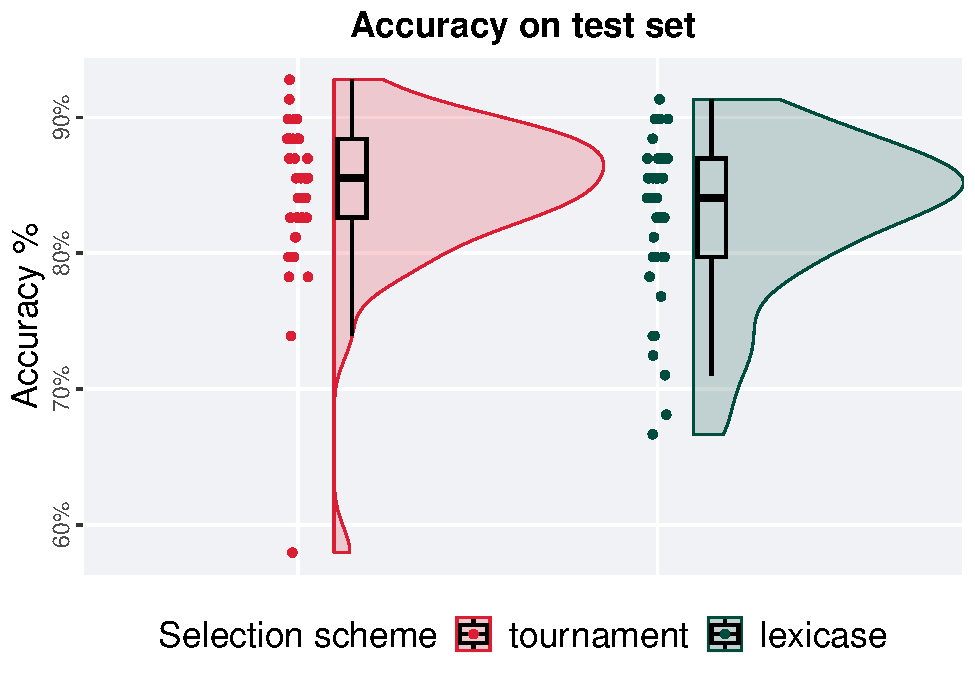
\includegraphics[width=1\linewidth]{lexidate-holdout-supplemental_files/figure-latex/task-146818-test-05-perf-1}

Summary statistics for the testing performance of the selection schemes at the 5\% selection set split:

\begin{Shaded}
\begin{Highlighting}[]
\FunctionTok{test\_results\_summary}\NormalTok{(}\FunctionTok{filter}\NormalTok{(task\_data, split }\SpecialCharTok{==} \StringTok{\textquotesingle{}5\%\textquotesingle{}}\NormalTok{))}
\end{Highlighting}
\end{Shaded}

\begin{verbatim}
## # A tibble: 2 x 8
##   selection  count na_cnt   min median  mean   max    IQR
##   <fct>      <int>  <int> <dbl>  <dbl> <dbl> <dbl>  <dbl>
## 1 tournament    40      0 0.580  0.855 0.845 0.928 0.0580
## 2 lexicase      40      0 0.667  0.841 0.826 0.913 0.0725
\end{verbatim}

The permutation test revealed that the results are:

\begin{Shaded}
\begin{Highlighting}[]
\NormalTok{tournament\_results }\OtherTok{\textless{}{-}} \FunctionTok{filter}\NormalTok{(task\_data, split }\SpecialCharTok{==} \StringTok{\textquotesingle{}5\%\textquotesingle{}} \SpecialCharTok{\&}\NormalTok{ selection }\SpecialCharTok{==} \StringTok{\textquotesingle{}tournament\textquotesingle{}}\NormalTok{)}
\NormalTok{lexicase\_results }\OtherTok{\textless{}{-}} \FunctionTok{filter}\NormalTok{(task\_data, split }\SpecialCharTok{==} \StringTok{\textquotesingle{}5\%\textquotesingle{}} \SpecialCharTok{\&}\NormalTok{ selection }\SpecialCharTok{==} \StringTok{\textquotesingle{}lexicase\textquotesingle{}}\NormalTok{)}
\FunctionTok{permutation\_test}\NormalTok{(tournament\_results}\SpecialCharTok{$}\NormalTok{testing\_performance,}
\NormalTok{                    lexicase\_results}\SpecialCharTok{$}\NormalTok{testing\_performance,}
                    \AttributeTok{seed =} \DecValTok{1}\NormalTok{,}
                    \AttributeTok{alternative =} \StringTok{"t"}\NormalTok{)}
\end{Highlighting}
\end{Shaded}

\begin{verbatim}
## [1] "observed_diff: 1.42058620905175"
## [1] "lower: -1.99072649993754"
## [1] "upper: 1.99072649993754"
## [1] "fail to reject null hypothesis"
## [1] "p-value: 0.15934"
\end{verbatim}

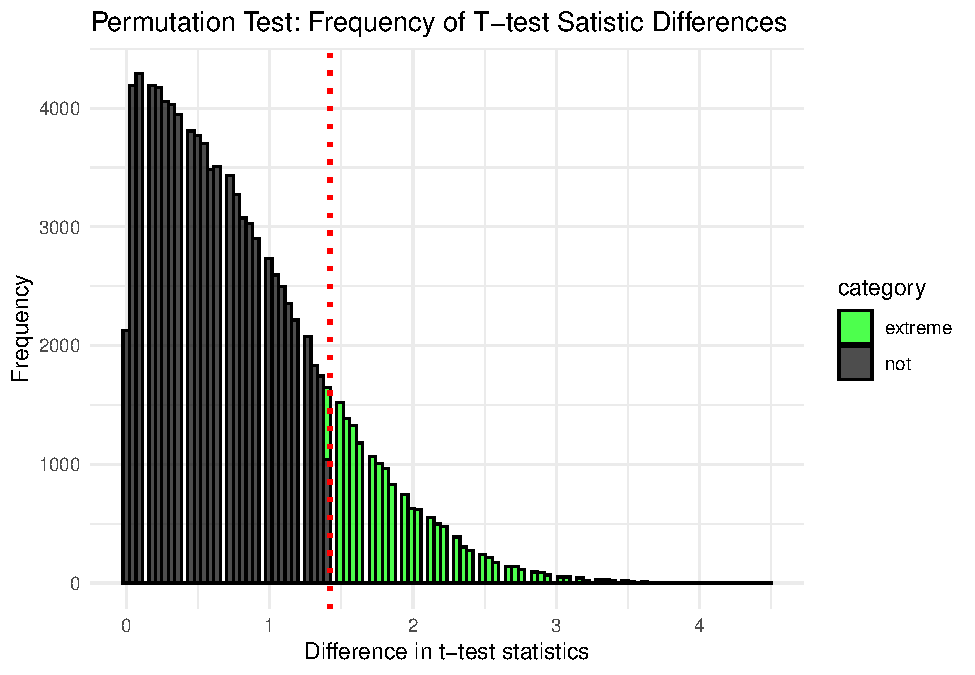
\includegraphics[width=1\linewidth]{lexidate-holdout-supplemental_files/figure-latex/task-146818-test-05-pv-1}

\hypertarget{selection-set-accuracy}{%
\subsection{Selection set accuracy}\label{selection-set-accuracy}}

\begin{Shaded}
\begin{Highlighting}[]
\FunctionTok{selection\_plot}\NormalTok{(}\FunctionTok{filter}\NormalTok{(task\_data, split }\SpecialCharTok{==} \StringTok{\textquotesingle{}5\%\textquotesingle{}}\NormalTok{))}
\end{Highlighting}
\end{Shaded}

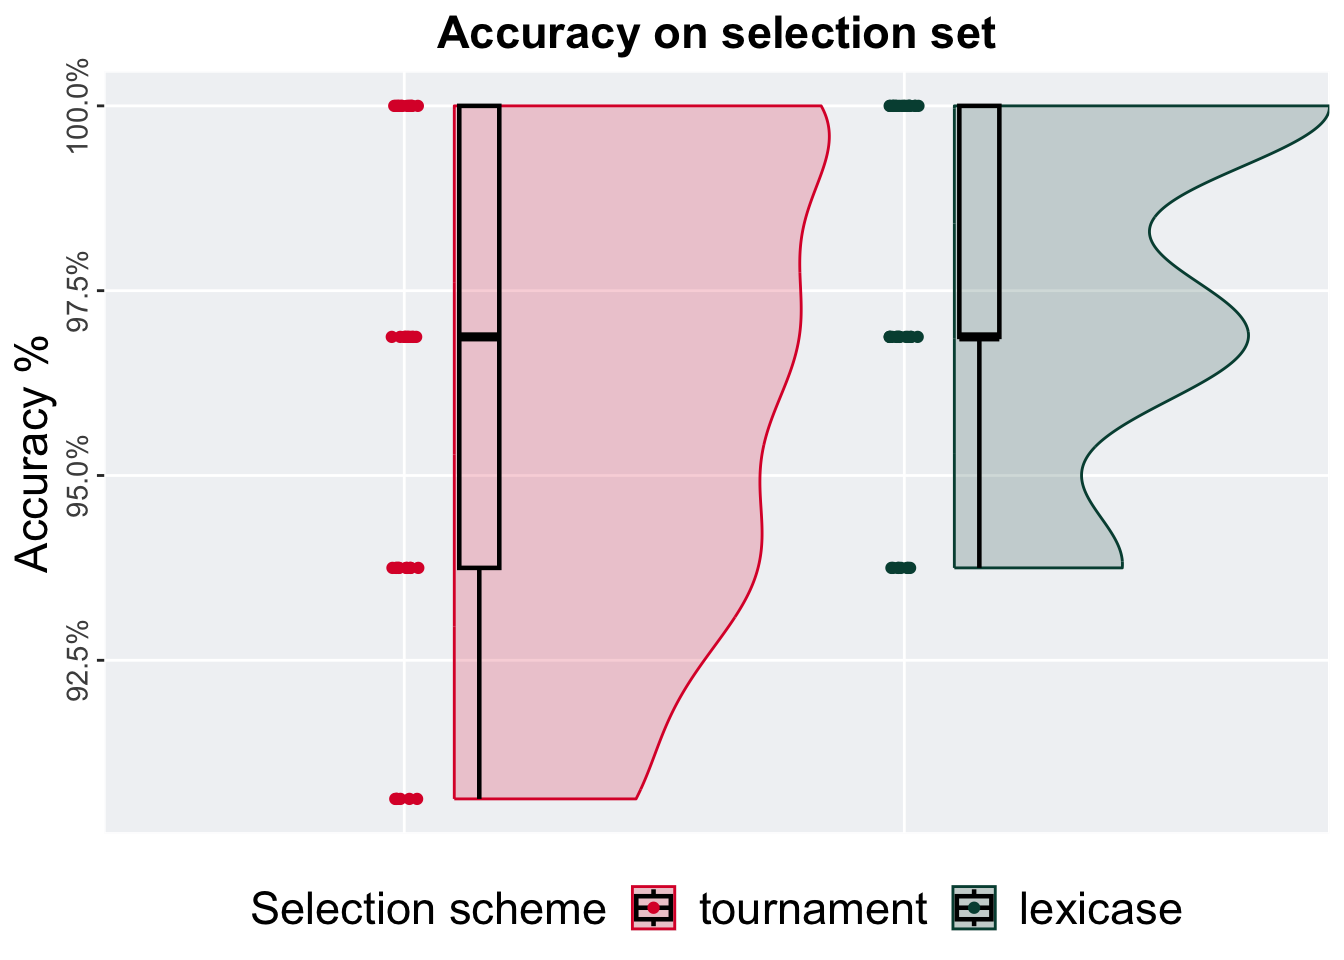
\includegraphics[width=1\linewidth]{lexidate-holdout-supplemental_files/figure-latex/task-146818-select-05-perf-1}

Summary statistics for the testing performance of the selection schemes at the 5\% selection set split:

\begin{Shaded}
\begin{Highlighting}[]
\FunctionTok{selection\_results\_summary}\NormalTok{(}\FunctionTok{filter}\NormalTok{(task\_data, split }\SpecialCharTok{==} \StringTok{\textquotesingle{}5\%\textquotesingle{}}\NormalTok{))}
\end{Highlighting}
\end{Shaded}

\begin{verbatim}
## # A tibble: 2 x 8
##   selection  count na_cnt   min median  mean   max    IQR
##   <fct>      <int>  <int> <dbl>  <dbl> <dbl> <dbl>  <dbl>
## 1 tournament    40      0 0.906  0.969 0.962     1 0.0625
## 2 lexicase      40      0 0.938  0.969 0.977     1 0.0312
\end{verbatim}

The permutation test revealed that the results are:

\begin{Shaded}
\begin{Highlighting}[]
\NormalTok{tournament\_results }\OtherTok{\textless{}{-}} \FunctionTok{filter}\NormalTok{(task\_data, split }\SpecialCharTok{==} \StringTok{\textquotesingle{}5\%\textquotesingle{}} \SpecialCharTok{\&}\NormalTok{ selection }\SpecialCharTok{==} \StringTok{\textquotesingle{}tournament\textquotesingle{}}\NormalTok{)}
\NormalTok{lexicase\_results }\OtherTok{\textless{}{-}} \FunctionTok{filter}\NormalTok{(task\_data, split }\SpecialCharTok{==} \StringTok{\textquotesingle{}5\%\textquotesingle{}} \SpecialCharTok{\&}\NormalTok{ selection }\SpecialCharTok{==} \StringTok{\textquotesingle{}lexicase\textquotesingle{}}\NormalTok{)}
\FunctionTok{permutation\_test}\NormalTok{(tournament\_results}\SpecialCharTok{$}\NormalTok{training\_performance,}
\NormalTok{                    lexicase\_results}\SpecialCharTok{$}\NormalTok{training\_performance,}
                    \AttributeTok{seed =} \DecValTok{2}\NormalTok{,}
                    \AttributeTok{alternative =} \StringTok{"l"}\NormalTok{)}
\end{Highlighting}
\end{Shaded}

\begin{verbatim}
## [1] "observed_diff: -2.26720028939778"
## [1] "permutation_diffs[0.05 * n_permutations]: -1.76808181038323"
## [1] "reject null hypothesis"
## [1] "p-value: 0.01586"
\end{verbatim}

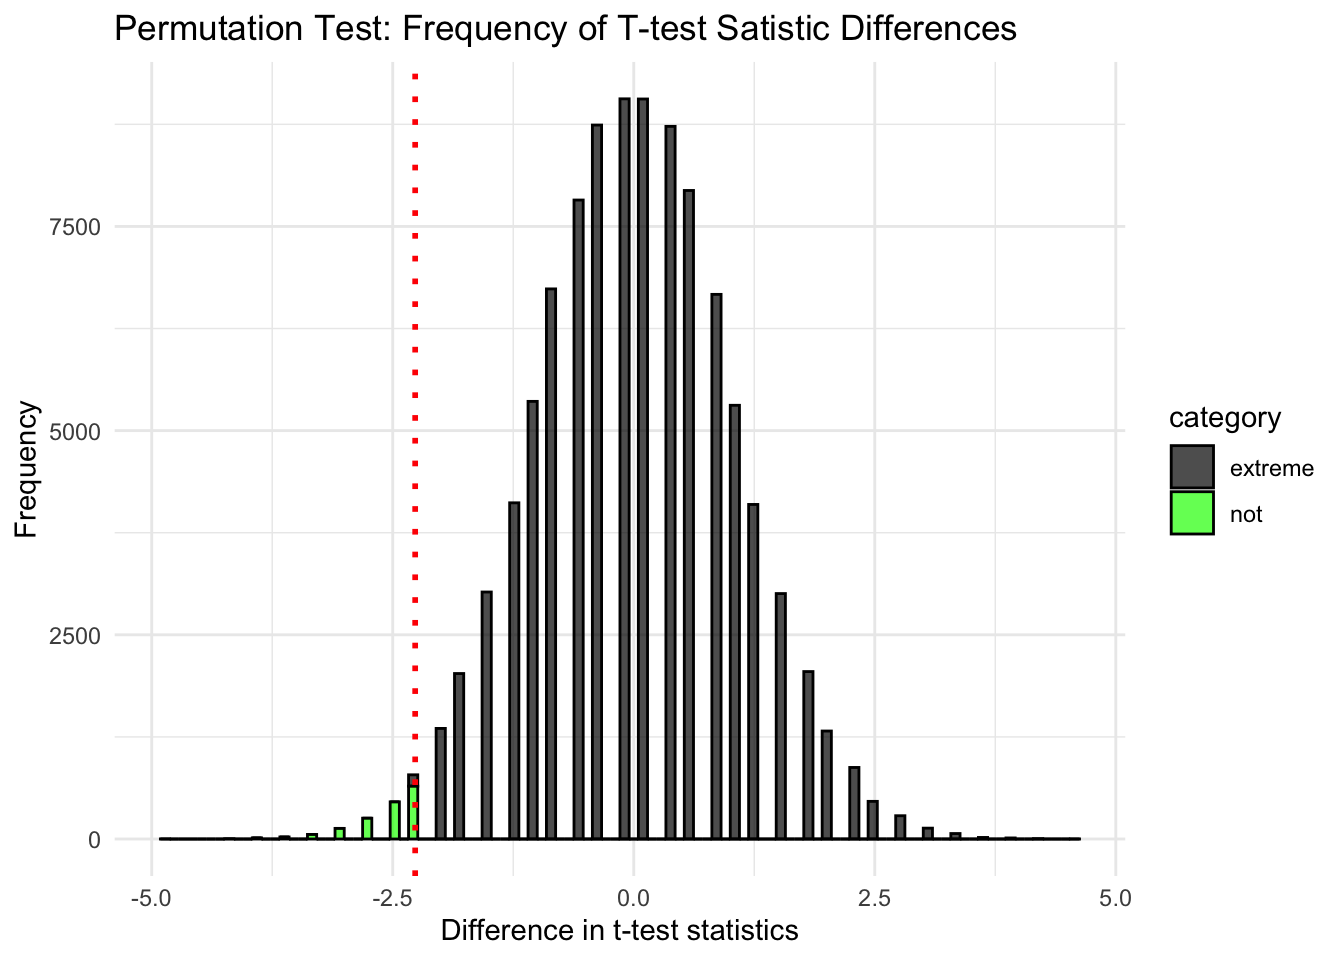
\includegraphics[width=1\linewidth]{lexidate-holdout-supplemental_files/figure-latex/task-146818-select-05-pv-1}

\hypertarget{section-1}\label{section-1}}

\hypertarget{testing-set-accuracy-1}{%
\subsection{Testing set accuracy}\label{testing-set-accuracy-1}}

\begin{Shaded}
\begin{Highlighting}[]
\FunctionTok{test\_plot}\NormalTok{(}\FunctionTok{filter}\NormalTok{(task\_data, split }\SpecialCharTok{==} \StringTok{\textquotesingle{}10\%\textquotesingle{}}\NormalTok{))}
\end{Highlighting}
\end{Shaded}

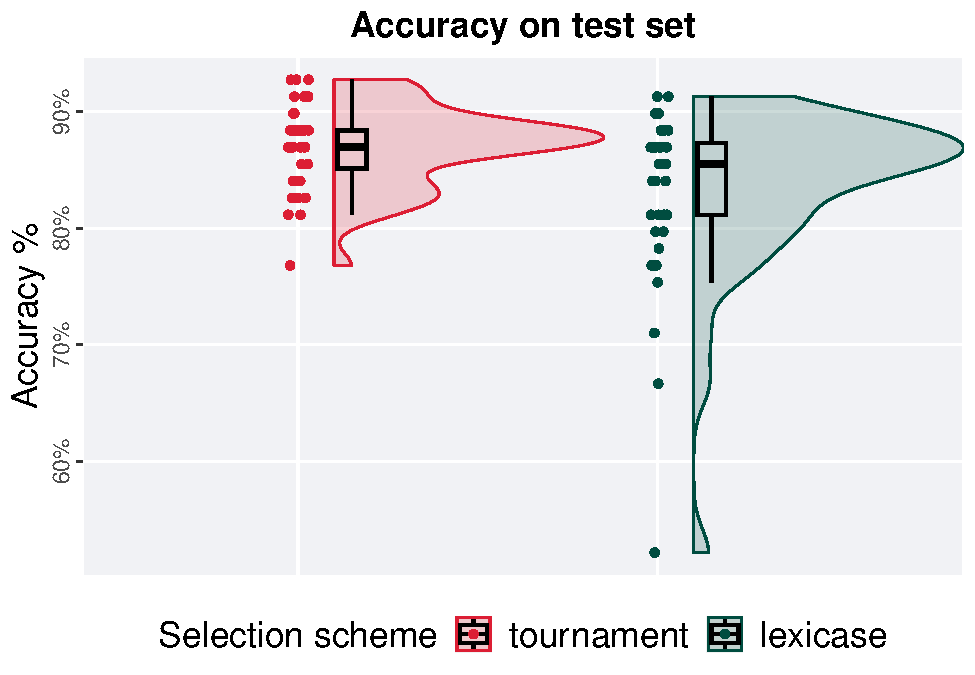
\includegraphics[width=1\linewidth]{lexidate-holdout-supplemental_files/figure-latex/task-146818-test-10-perf-1}

Summary statistics for the testing performance of the selection schemes at the 5\% selection set split:

\begin{Shaded}
\begin{Highlighting}[]
\FunctionTok{test\_results\_summary}\NormalTok{(}\FunctionTok{filter}\NormalTok{(task\_data, split }\SpecialCharTok{==} \StringTok{\textquotesingle{}10\%\textquotesingle{}}\NormalTok{))}
\end{Highlighting}
\end{Shaded}

\begin{verbatim}
## # A tibble: 2 x 8
##   selection  count na_cnt   min median  mean   max    IQR
##   <fct>      <int>  <int> <dbl>  <dbl> <dbl> <dbl>  <dbl>
## 1 tournament    40      0 0.768  0.870 0.870 0.928 0.0326
## 2 lexicase      40      0 0.522  0.855 0.834 0.913 0.0616
\end{verbatim}

The permutation test revealed that the results are:

\begin{Shaded}
\begin{Highlighting}[]
\NormalTok{tournament\_results }\OtherTok{\textless{}{-}} \FunctionTok{filter}\NormalTok{(task\_data, split }\SpecialCharTok{==} \StringTok{\textquotesingle{}10\%\textquotesingle{}} \SpecialCharTok{\&}\NormalTok{ selection }\SpecialCharTok{==} \StringTok{\textquotesingle{}tournament\textquotesingle{}}\NormalTok{)}
\NormalTok{lexicase\_results }\OtherTok{\textless{}{-}} \FunctionTok{filter}\NormalTok{(task\_data, split }\SpecialCharTok{==} \StringTok{\textquotesingle{}10\%\textquotesingle{}} \SpecialCharTok{\&}\NormalTok{ selection }\SpecialCharTok{==} \StringTok{\textquotesingle{}lexicase\textquotesingle{}}\NormalTok{)}
\FunctionTok{permutation\_test}\NormalTok{(tournament\_results}\SpecialCharTok{$}\NormalTok{testing\_performance,}
\NormalTok{                    lexicase\_results}\SpecialCharTok{$}\NormalTok{testing\_performance,}
                    \AttributeTok{seed =} \DecValTok{3}\NormalTok{,}
                    \AttributeTok{alternative =} \StringTok{"g"}\NormalTok{)}
\end{Highlighting}
\end{Shaded}

\begin{verbatim}
## [1] "observed_diff: 2.82771300817792"
## [1] "permutation_diffs[0.95 * n_permutations]: 1.65479687273561"
## [1] "reject null hypothesis"
## [1] "p-value: 0.00146"
\end{verbatim}

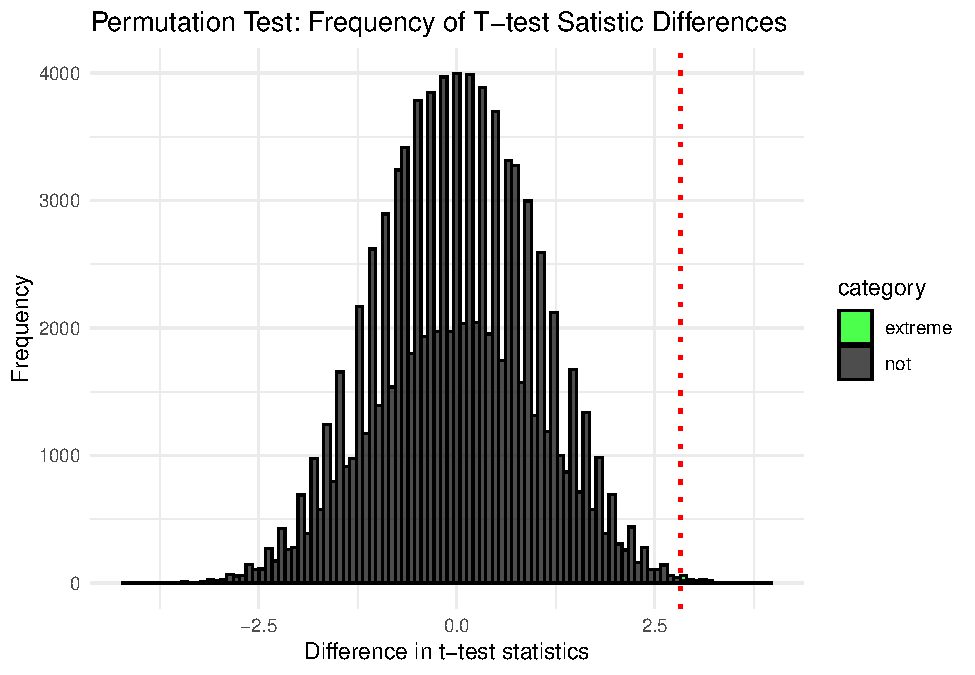
\includegraphics[width=1\linewidth]{lexidate-holdout-supplemental_files/figure-latex/task-146818-test-10-pv-1}

\hypertarget{selection-set-accuracy-1}{%
\subsection{Selection set accuracy}\label{selection-set-accuracy-1}}

\begin{Shaded}
\begin{Highlighting}[]
\FunctionTok{selection\_plot}\NormalTok{(}\FunctionTok{filter}\NormalTok{(task\_data, split }\SpecialCharTok{==} \StringTok{\textquotesingle{}10\%\textquotesingle{}}\NormalTok{))}
\end{Highlighting}
\end{Shaded}

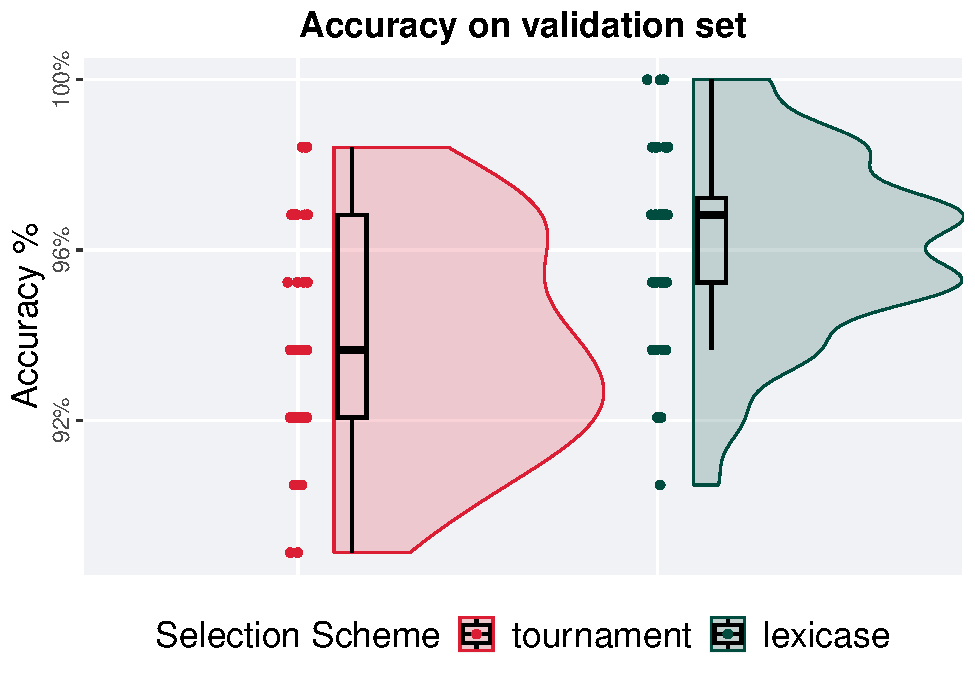
\includegraphics[width=1\linewidth]{lexidate-holdout-supplemental_files/figure-latex/task-146818-select-10-perf-1}

Summary statistics for the testing performance of the selection schemes at the 5\% selection set split:

\begin{Shaded}
\begin{Highlighting}[]
\FunctionTok{selection\_results\_summary}\NormalTok{(}\FunctionTok{filter}\NormalTok{(task\_data, split }\SpecialCharTok{==} \StringTok{\textquotesingle{}10\%\textquotesingle{}}\NormalTok{))}
\end{Highlighting}
\end{Shaded}

\begin{verbatim}
## # A tibble: 2 x 8
##   selection  count na_cnt   min median  mean   max    IQR
##   <fct>      <int>  <int> <dbl>  <dbl> <dbl> <dbl>  <dbl>
## 1 tournament    40      0 0.889  0.937 0.938 0.984 0.0476
## 2 lexicase      40      0 0.905  0.968 0.961 1     0.0198
\end{verbatim}

The permutation test revealed that the results are:

\begin{Shaded}
\begin{Highlighting}[]
\NormalTok{tournament\_results }\OtherTok{\textless{}{-}} \FunctionTok{filter}\NormalTok{(task\_data, split }\SpecialCharTok{==} \StringTok{\textquotesingle{}10\%\textquotesingle{}} \SpecialCharTok{\&}\NormalTok{ selection }\SpecialCharTok{==} \StringTok{\textquotesingle{}tournament\textquotesingle{}}\NormalTok{)}
\NormalTok{lexicase\_results }\OtherTok{\textless{}{-}} \FunctionTok{filter}\NormalTok{(task\_data, split }\SpecialCharTok{==} \StringTok{\textquotesingle{}10\%\textquotesingle{}} \SpecialCharTok{\&}\NormalTok{ selection }\SpecialCharTok{==} \StringTok{\textquotesingle{}lexicase\textquotesingle{}}\NormalTok{)}
\FunctionTok{permutation\_test}\NormalTok{(tournament\_results}\SpecialCharTok{$}\NormalTok{training\_performance,}
\NormalTok{                    lexicase\_results}\SpecialCharTok{$}\NormalTok{training\_performance,}
                    \AttributeTok{seed =} \DecValTok{4}\NormalTok{,}
                    \AttributeTok{alternative =} \StringTok{"l"}\NormalTok{)}
\end{Highlighting}
\end{Shaded}

\begin{verbatim}
## [1] "observed_diff: -4.12382195839694"
## [1] "permutation_diffs[0.05 * n_permutations]: -1.66780738405742"
## [1] "reject null hypothesis"
## [1] "p-value: 2e-05"
\end{verbatim}

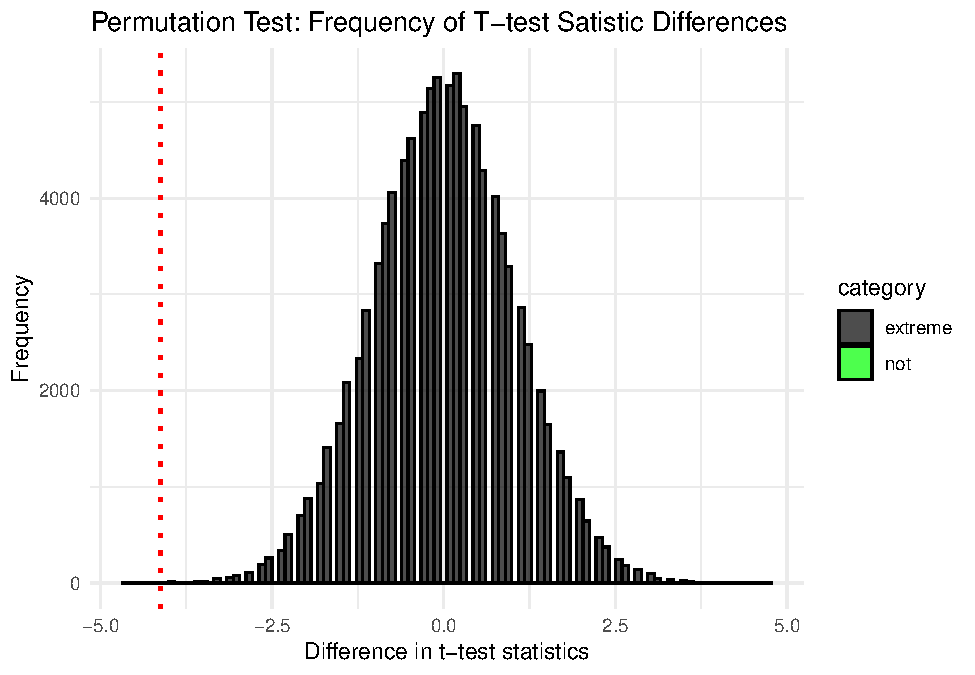
\includegraphics[width=1\linewidth]{lexidate-holdout-supplemental_files/figure-latex/task-146818-select-10-pv-1}

\hypertarget{section-2}\label{section-2}}

\hypertarget{testing-set-accuracy-2}{%
\subsection{Testing set accuracy}\label{testing-set-accuracy-2}}

\begin{Shaded}
\begin{Highlighting}[]
\FunctionTok{test\_plot}\NormalTok{(}\FunctionTok{filter}\NormalTok{(task\_data, split }\SpecialCharTok{==} \StringTok{\textquotesingle{}50\%\textquotesingle{}}\NormalTok{))}
\end{Highlighting}
\end{Shaded}

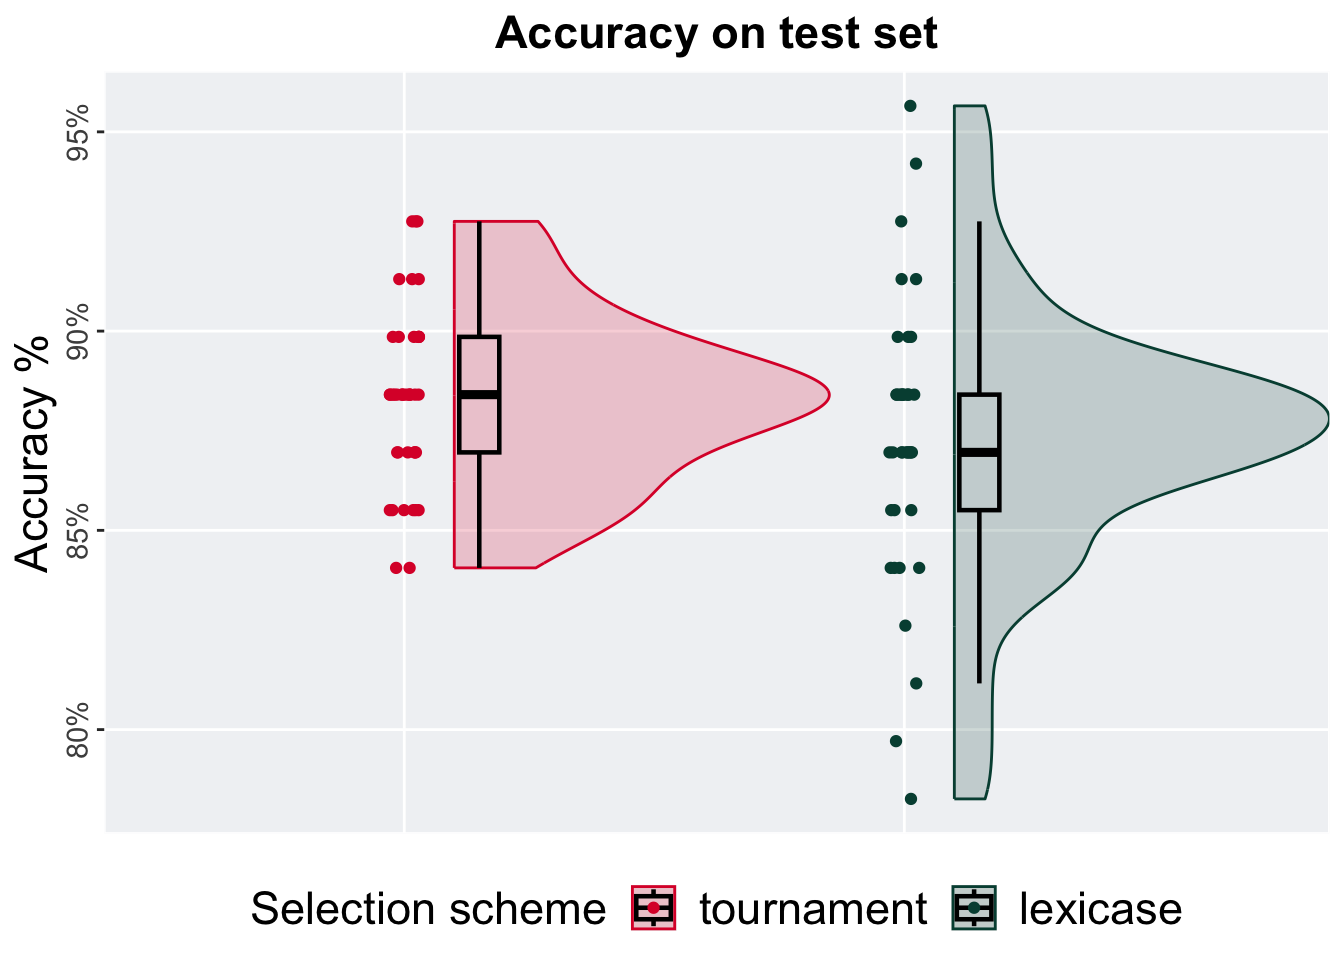
\includegraphics[width=1\linewidth]{lexidate-holdout-supplemental_files/figure-latex/task-146818-test-50-perf-1}

Summary statistics for the testing performance of the selection schemes at the 5\% selection set split:

\begin{Shaded}
\begin{Highlighting}[]
\FunctionTok{test\_results\_summary}\NormalTok{(}\FunctionTok{filter}\NormalTok{(task\_data, split }\SpecialCharTok{==} \StringTok{\textquotesingle{}50\%\textquotesingle{}}\NormalTok{))}
\end{Highlighting}
\end{Shaded}

\begin{verbatim}
## # A tibble: 2 x 8
##   selection  count na_cnt   min median  mean   max    IQR
##   <fct>      <int>  <int> <dbl>  <dbl> <dbl> <dbl>  <dbl>
## 1 tournament    40      0 0.841  0.884 0.883 0.928 0.0290
## 2 lexicase      40      0 0.783  0.870 0.873 0.957 0.0290
\end{verbatim}

The permutation test revealed that the results are:

\begin{Shaded}
\begin{Highlighting}[]
\NormalTok{tournament\_results }\OtherTok{\textless{}{-}} \FunctionTok{filter}\NormalTok{(task\_data, split }\SpecialCharTok{==} \StringTok{\textquotesingle{}50\%\textquotesingle{}} \SpecialCharTok{\&}\NormalTok{ selection }\SpecialCharTok{==} \StringTok{\textquotesingle{}tournament\textquotesingle{}}\NormalTok{)}
\NormalTok{lexicase\_results }\OtherTok{\textless{}{-}} \FunctionTok{filter}\NormalTok{(task\_data, split }\SpecialCharTok{==} \StringTok{\textquotesingle{}50\%\textquotesingle{}} \SpecialCharTok{\&}\NormalTok{ selection }\SpecialCharTok{==} \StringTok{\textquotesingle{}lexicase\textquotesingle{}}\NormalTok{)}
\FunctionTok{permutation\_test}\NormalTok{(tournament\_results}\SpecialCharTok{$}\NormalTok{testing\_performance,}
\NormalTok{                    lexicase\_results}\SpecialCharTok{$}\NormalTok{testing\_performance,}
                    \AttributeTok{seed =} \DecValTok{5}\NormalTok{,}
                    \AttributeTok{alternative =} \StringTok{"t"}\NormalTok{)}
\end{Highlighting}
\end{Shaded}

\begin{verbatim}
## [1] "observed_diff: 1.5608765017161"
## [1] "lower: -2.02762682929956"
## [1] "upper: 2.02762732023459"
## [1] "fail to reject null hypothesis"
## [1] "p-value: 0.11875"
\end{verbatim}

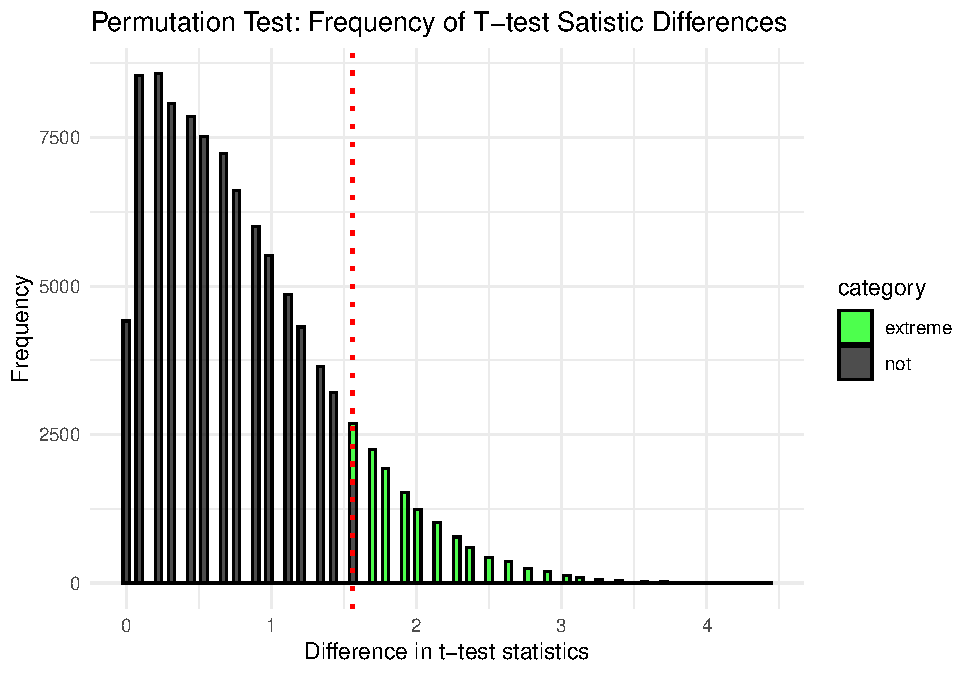
\includegraphics[width=1\linewidth]{lexidate-holdout-supplemental_files/figure-latex/task-146818-test-50-pv-1}

\hypertarget{selection-set-accuracy-2}{%
\subsection{Selection set accuracy}\label{selection-set-accuracy-2}}

\begin{Shaded}
\begin{Highlighting}[]
\FunctionTok{selection\_plot}\NormalTok{(}\FunctionTok{filter}\NormalTok{(task\_data, split }\SpecialCharTok{==} \StringTok{\textquotesingle{}50\%\textquotesingle{}}\NormalTok{))}
\end{Highlighting}
\end{Shaded}

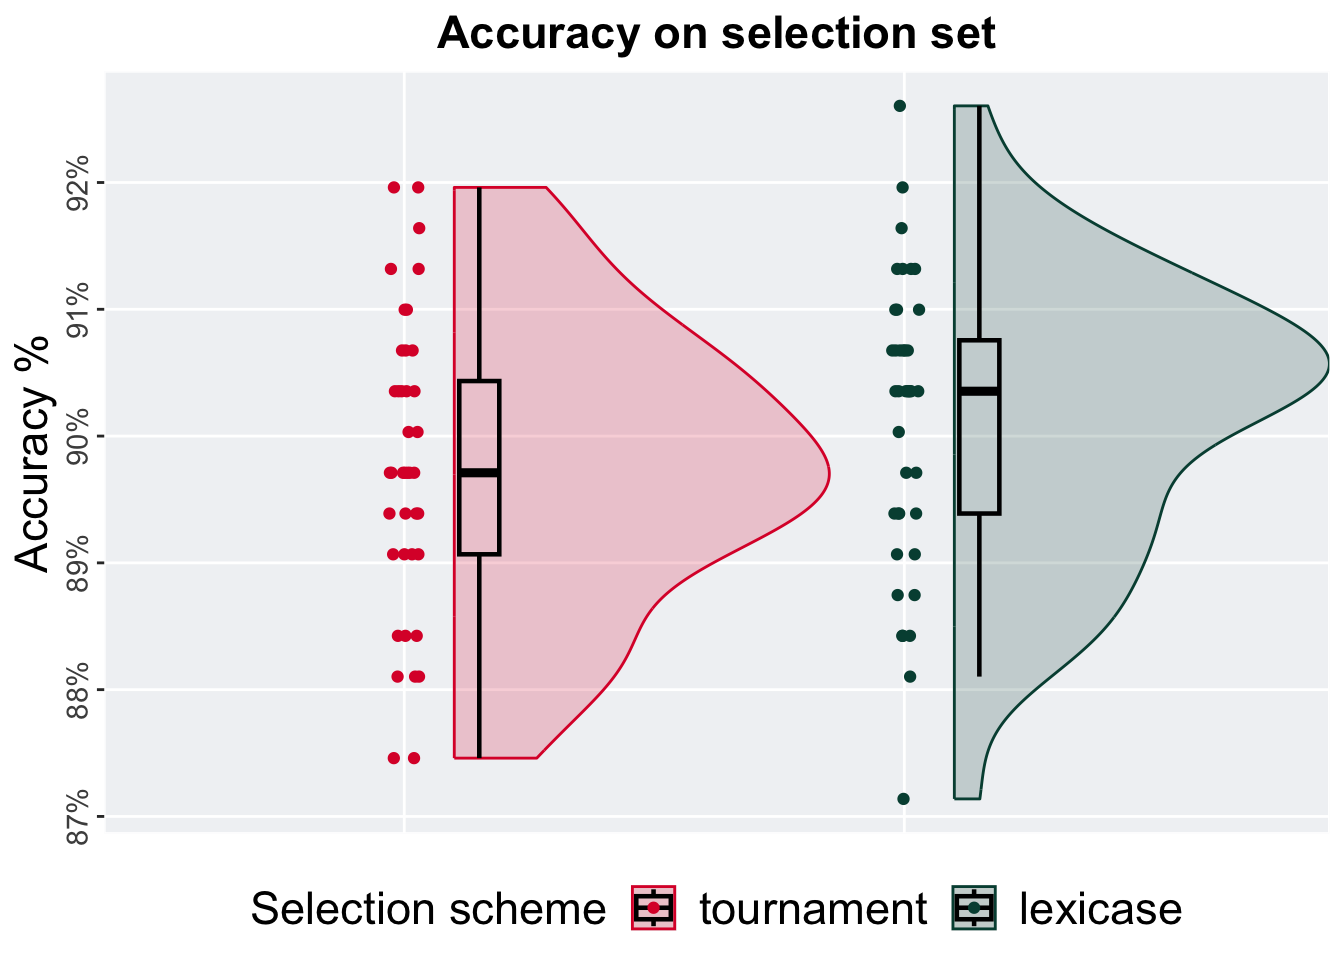
\includegraphics[width=1\linewidth]{lexidate-holdout-supplemental_files/figure-latex/task-146818-select-50-perf-1}

Summary statistics for the testing performance of the selection schemes at the 5\% selection set split:

\begin{Shaded}
\begin{Highlighting}[]
\FunctionTok{selection\_results\_summary}\NormalTok{(}\FunctionTok{filter}\NormalTok{(task\_data, split }\SpecialCharTok{==} \StringTok{\textquotesingle{}50\%\textquotesingle{}}\NormalTok{))}
\end{Highlighting}
\end{Shaded}

\begin{verbatim}
## # A tibble: 2 x 8
##   selection  count na_cnt   min median  mean   max    IQR
##   <fct>      <int>  <int> <dbl>  <dbl> <dbl> <dbl>  <dbl>
## 1 tournament    40      0 0.875  0.897 0.898 0.920 0.0137
## 2 lexicase      40      0 0.871  0.904 0.901 0.926 0.0137
\end{verbatim}

The permutation test revealed that the results are:

\begin{Shaded}
\begin{Highlighting}[]
\NormalTok{tournament\_results }\OtherTok{\textless{}{-}} \FunctionTok{filter}\NormalTok{(task\_data, split }\SpecialCharTok{==} \StringTok{\textquotesingle{}50\%\textquotesingle{}} \SpecialCharTok{\&}\NormalTok{ selection }\SpecialCharTok{==} \StringTok{\textquotesingle{}tournament\textquotesingle{}}\NormalTok{)}
\NormalTok{lexicase\_results }\OtherTok{\textless{}{-}} \FunctionTok{filter}\NormalTok{(task\_data, split }\SpecialCharTok{==} \StringTok{\textquotesingle{}50\%\textquotesingle{}} \SpecialCharTok{\&}\NormalTok{ selection }\SpecialCharTok{==} \StringTok{\textquotesingle{}lexicase\textquotesingle{}}\NormalTok{)}
\FunctionTok{permutation\_test}\NormalTok{(tournament\_results}\SpecialCharTok{$}\NormalTok{training\_performance,}
\NormalTok{                    lexicase\_results}\SpecialCharTok{$}\NormalTok{training\_performance,}
                    \AttributeTok{seed =} \DecValTok{6}\NormalTok{,}
                    \AttributeTok{alternative =} \StringTok{"t"}\NormalTok{)}
\end{Highlighting}
\end{Shaded}

\begin{verbatim}
## [1] "observed_diff: -1.3666761390605"
## [1] "lower: -2.01498791705763"
## [1] "upper: 2.01499018334096"
## [1] "fail to reject null hypothesis"
## [1] "p-value: 0.16869"
\end{verbatim}

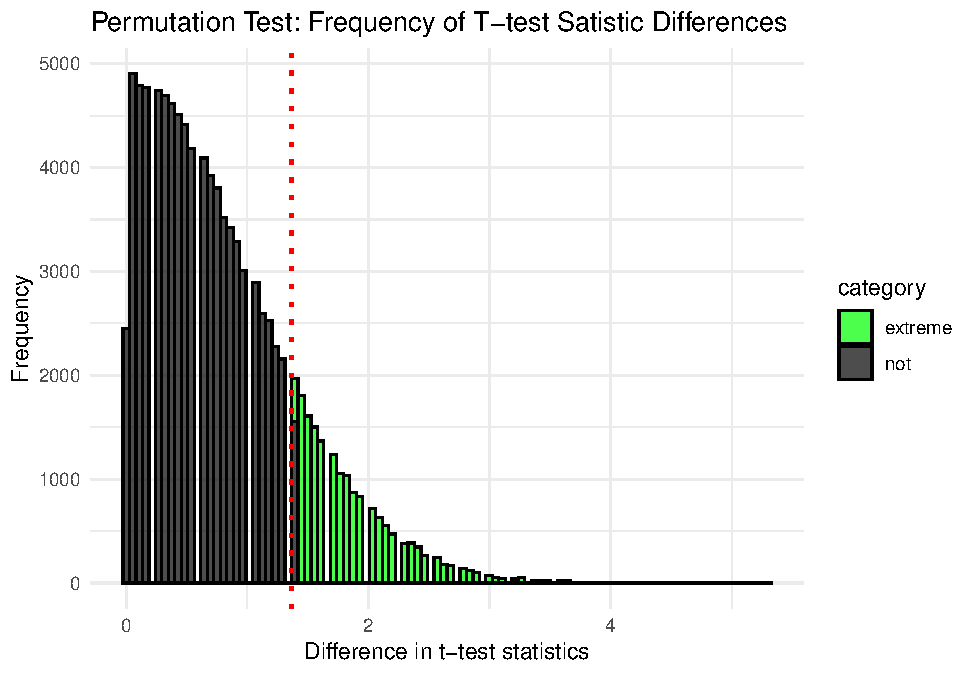
\includegraphics[width=1\linewidth]{lexidate-holdout-supplemental_files/figure-latex/task-146818-select-50-pv-1}

\hypertarget{section-3}\label{section-3}}

\hypertarget{testing-set-accuracy-3}{%
\subsection{Testing set accuracy}\label{testing-set-accuracy-3}}

\begin{Shaded}
\begin{Highlighting}[]
\FunctionTok{test\_plot}\NormalTok{(}\FunctionTok{filter}\NormalTok{(task\_data, split }\SpecialCharTok{==} \StringTok{\textquotesingle{}90\%\textquotesingle{}}\NormalTok{))}
\end{Highlighting}
\end{Shaded}

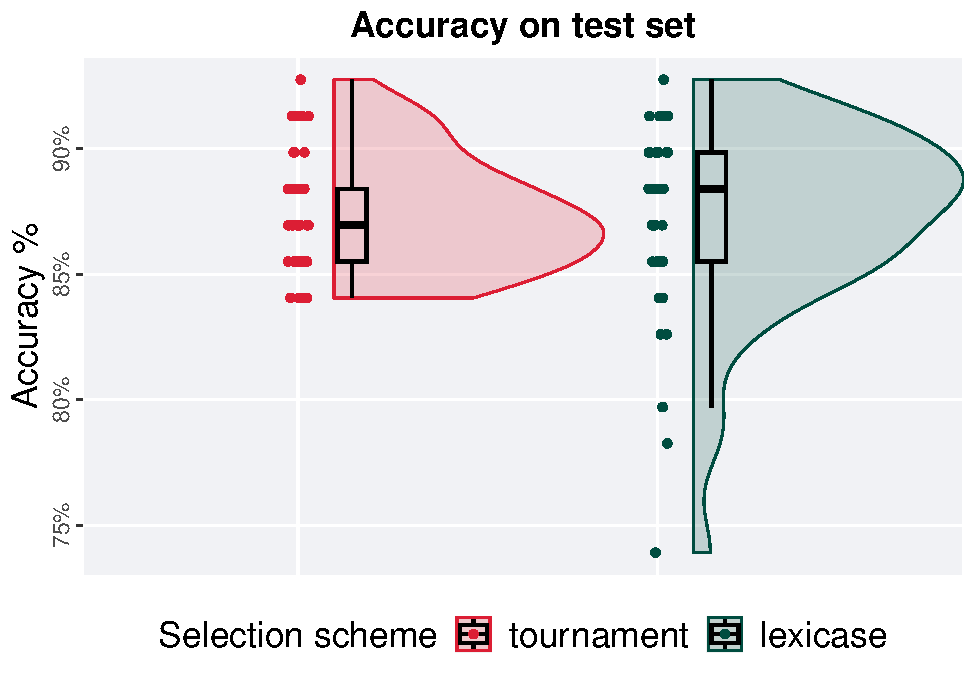
\includegraphics[width=1\linewidth]{lexidate-holdout-supplemental_files/figure-latex/task-146818-test-90-perf-1}

Summary statistics for the testing performance of the selection schemes at the 5\% selection set split:

\begin{Shaded}
\begin{Highlighting}[]
\FunctionTok{test\_results\_summary}\NormalTok{(}\FunctionTok{filter}\NormalTok{(task\_data, split }\SpecialCharTok{==} \StringTok{\textquotesingle{}90\%\textquotesingle{}}\NormalTok{))}
\end{Highlighting}
\end{Shaded}

\begin{verbatim}
## # A tibble: 2 x 8
##   selection  count na_cnt   min median  mean   max    IQR
##   <fct>      <int>  <int> <dbl>  <dbl> <dbl> <dbl>  <dbl>
## 1 tournament    40      0 0.841  0.870 0.874 0.928 0.0290
## 2 lexicase      40      0 0.739  0.884 0.872 0.928 0.0435
\end{verbatim}

The permutation test revealed that the results are:

\begin{Shaded}
\begin{Highlighting}[]
\NormalTok{tournament\_results }\OtherTok{\textless{}{-}} \FunctionTok{filter}\NormalTok{(task\_data, split }\SpecialCharTok{==} \StringTok{\textquotesingle{}90\%\textquotesingle{}} \SpecialCharTok{\&}\NormalTok{ selection }\SpecialCharTok{==} \StringTok{\textquotesingle{}tournament\textquotesingle{}}\NormalTok{)}
\NormalTok{lexicase\_results }\OtherTok{\textless{}{-}} \FunctionTok{filter}\NormalTok{(task\_data, split }\SpecialCharTok{==} \StringTok{\textquotesingle{}90\%\textquotesingle{}} \SpecialCharTok{\&}\NormalTok{ selection }\SpecialCharTok{==} \StringTok{\textquotesingle{}lexicase\textquotesingle{}}\NormalTok{)}
\FunctionTok{permutation\_test}\NormalTok{(tournament\_results}\SpecialCharTok{$}\NormalTok{testing\_performance,}
\NormalTok{                    lexicase\_results}\SpecialCharTok{$}\NormalTok{testing\_performance,}
                    \AttributeTok{seed =} \DecValTok{7}\NormalTok{,}
                    \AttributeTok{alternative =} \StringTok{"t"}\NormalTok{)}
\end{Highlighting}
\end{Shaded}

\begin{verbatim}
## [1] "observed_diff: 0.304925249770556"
## [1] "lower: -1.97785745966913"
## [1] "upper: 1.97785745966913"
## [1] "fail to reject null hypothesis"
## [1] "p-value: 0.80197"
\end{verbatim}

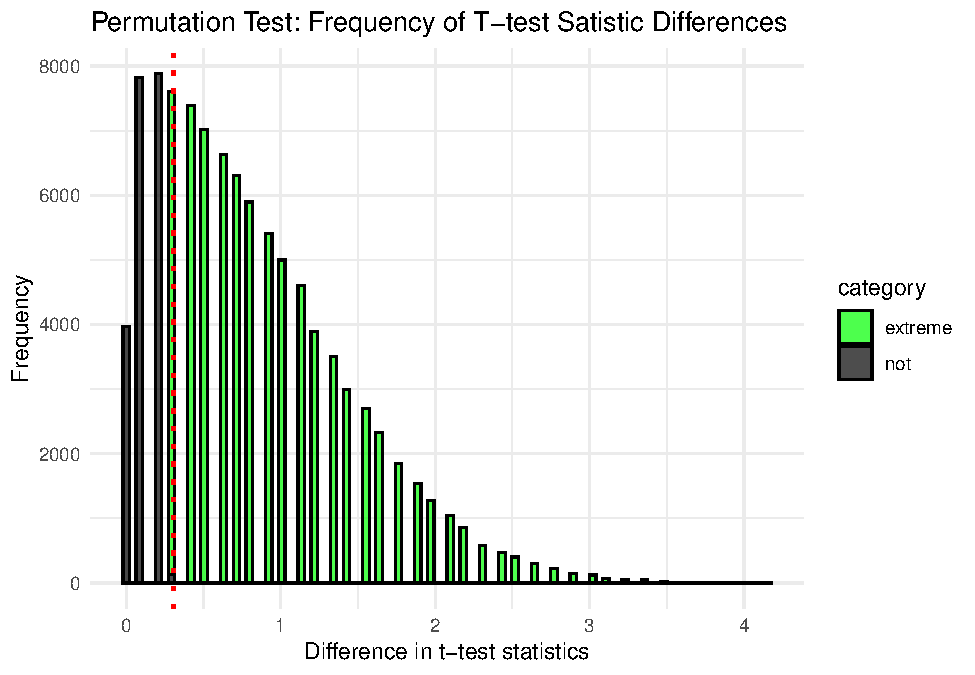
\includegraphics[width=1\linewidth]{lexidate-holdout-supplemental_files/figure-latex/task-146818-test-90-pv-1}

\hypertarget{selection-set-accuracy-3}{%
\subsection{Selection set accuracy}\label{selection-set-accuracy-3}}

\begin{Shaded}
\begin{Highlighting}[]
\FunctionTok{selection\_plot}\NormalTok{(}\FunctionTok{filter}\NormalTok{(task\_data, split }\SpecialCharTok{==} \StringTok{\textquotesingle{}90\%\textquotesingle{}}\NormalTok{))}
\end{Highlighting}
\end{Shaded}

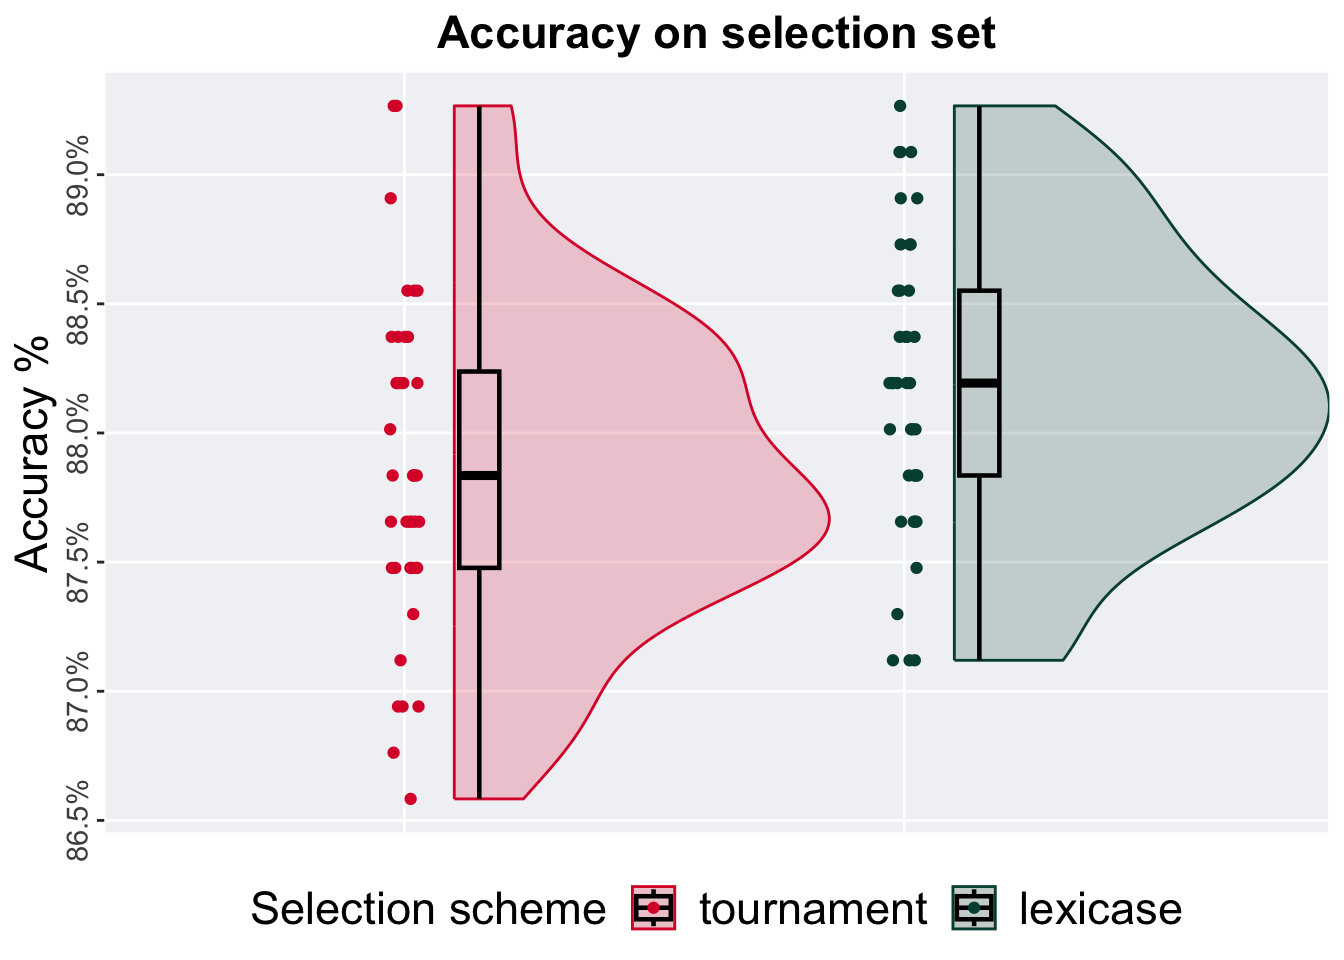
\includegraphics[width=1\linewidth]{lexidate-holdout-supplemental_files/figure-latex/task-146818-select-90-perf-1}

Summary statistics for the testing performance of the selection schemes at the 5\% selection set split:

\begin{Shaded}
\begin{Highlighting}[]
\FunctionTok{selection\_results\_summary}\NormalTok{(}\FunctionTok{filter}\NormalTok{(task\_data, split }\SpecialCharTok{==} \StringTok{\textquotesingle{}90\%\textquotesingle{}}\NormalTok{))}
\end{Highlighting}
\end{Shaded}

\begin{verbatim}
## # A tibble: 2 x 8
##   selection  count na_cnt   min median  mean   max     IQR
##   <fct>      <int>  <int> <dbl>  <dbl> <dbl> <dbl>   <dbl>
## 1 tournament    40      0 0.866  0.878 0.879 0.893 0.00760
## 2 lexicase      40      0 0.871  0.882 0.882 0.893 0.00716
\end{verbatim}

The permutation test revealed that the results are:

\begin{Shaded}
\begin{Highlighting}[]
\NormalTok{tournament\_results }\OtherTok{\textless{}{-}} \FunctionTok{filter}\NormalTok{(task\_data, split }\SpecialCharTok{==} \StringTok{\textquotesingle{}90\%\textquotesingle{}} \SpecialCharTok{\&}\NormalTok{ selection }\SpecialCharTok{==} \StringTok{\textquotesingle{}tournament\textquotesingle{}}\NormalTok{)}
\NormalTok{lexicase\_results }\OtherTok{\textless{}{-}} \FunctionTok{filter}\NormalTok{(task\_data, split }\SpecialCharTok{==} \StringTok{\textquotesingle{}90\%\textquotesingle{}} \SpecialCharTok{\&}\NormalTok{ selection }\SpecialCharTok{==} \StringTok{\textquotesingle{}lexicase\textquotesingle{}}\NormalTok{)}
\FunctionTok{permutation\_test}\NormalTok{(tournament\_results}\SpecialCharTok{$}\NormalTok{training\_performance,}
\NormalTok{                    lexicase\_results}\SpecialCharTok{$}\NormalTok{training\_performance,}
                    \AttributeTok{seed =} \DecValTok{8}\NormalTok{,}
                    \AttributeTok{alternative =} \StringTok{"l"}\NormalTok{)}
\end{Highlighting}
\end{Shaded}

\begin{verbatim}
## [1] "observed_diff: -2.3660300252374"
## [1] "permutation_diffs[0.05 * n_permutations]: -1.67076701407627"
## [1] "reject null hypothesis"
## [1] "p-value: 0.00964"
\end{verbatim}

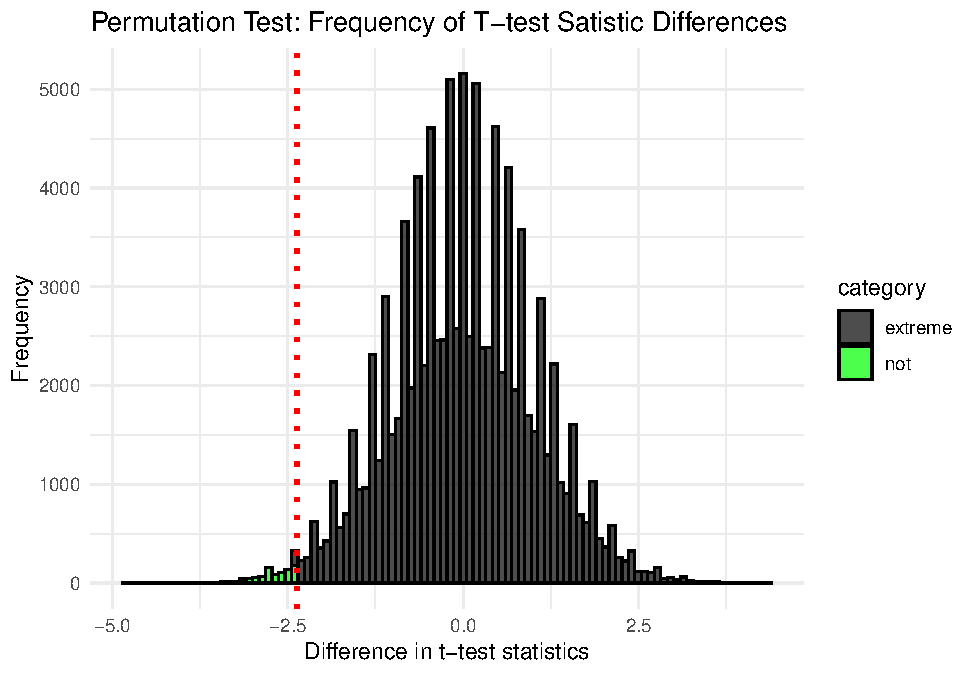
\includegraphics[width=1\linewidth]{lexidate-holdout-supplemental_files/figure-latex/task-146818-select-90-pv-1}

\hypertarget{section-4}\label{section-4}}

\hypertarget{testing-set-accuracy-4}{%
\subsection{Testing set accuracy}\label{testing-set-accuracy-4}}

\begin{Shaded}
\begin{Highlighting}[]
\FunctionTok{test\_plot}\NormalTok{(}\FunctionTok{filter}\NormalTok{(task\_data, split }\SpecialCharTok{==} \StringTok{\textquotesingle{}95\%\textquotesingle{}}\NormalTok{))}
\end{Highlighting}
\end{Shaded}

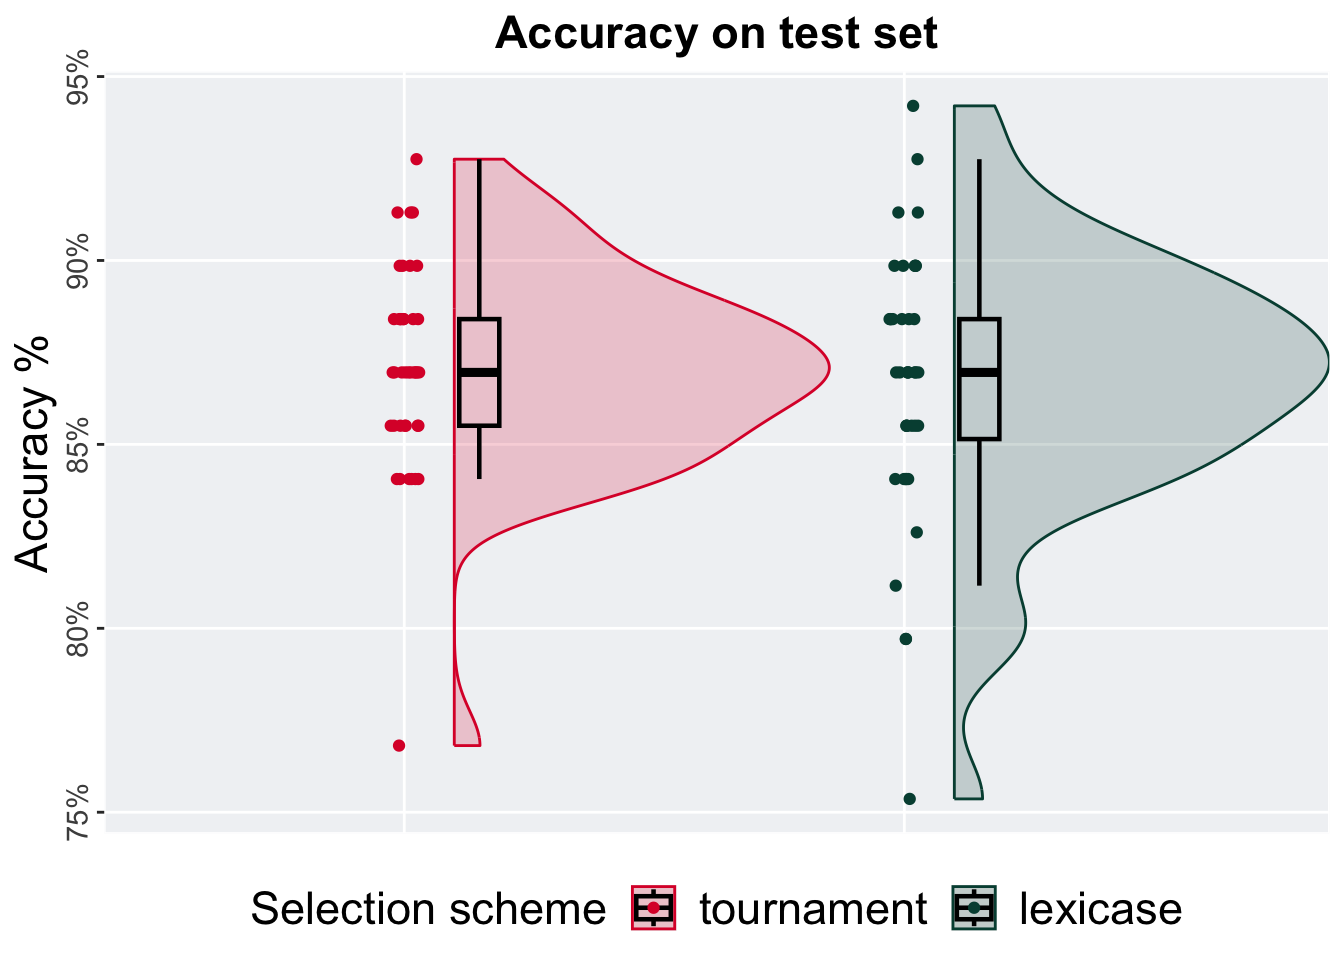
\includegraphics[width=1\linewidth]{lexidate-holdout-supplemental_files/figure-latex/task-146818-test-95-perf-1}

Summary statistics for the testing performance of the selection schemes at the 5\% selection set split:

\begin{Shaded}
\begin{Highlighting}[]
\FunctionTok{test\_results\_summary}\NormalTok{(}\FunctionTok{filter}\NormalTok{(task\_data, split }\SpecialCharTok{==} \StringTok{\textquotesingle{}95\%\textquotesingle{}}\NormalTok{))}
\end{Highlighting}
\end{Shaded}

\begin{verbatim}
## # A tibble: 2 x 8
##   selection  count na_cnt   min median  mean   max    IQR
##   <fct>      <int>  <int> <dbl>  <dbl> <dbl> <dbl>  <dbl>
## 1 tournament    40      0 0.768  0.870 0.871 0.928 0.0290
## 2 lexicase      40      0 0.754  0.870 0.866 0.942 0.0326
\end{verbatim}

The permutation test revealed that the results are:

\begin{Shaded}
\begin{Highlighting}[]
\NormalTok{tournament\_results }\OtherTok{\textless{}{-}} \FunctionTok{filter}\NormalTok{(task\_data, split }\SpecialCharTok{==} \StringTok{\textquotesingle{}95\%\textquotesingle{}} \SpecialCharTok{\&}\NormalTok{ selection }\SpecialCharTok{==} \StringTok{\textquotesingle{}tournament\textquotesingle{}}\NormalTok{)}
\NormalTok{lexicase\_results }\OtherTok{\textless{}{-}} \FunctionTok{filter}\NormalTok{(task\_data, split }\SpecialCharTok{==} \StringTok{\textquotesingle{}95\%\textquotesingle{}} \SpecialCharTok{\&}\NormalTok{ selection }\SpecialCharTok{==} \StringTok{\textquotesingle{}lexicase\textquotesingle{}}\NormalTok{)}
\FunctionTok{permutation\_test}\NormalTok{(tournament\_results}\SpecialCharTok{$}\NormalTok{testing\_performance,}
\NormalTok{                    lexicase\_results}\SpecialCharTok{$}\NormalTok{testing\_performance,}
                    \AttributeTok{seed =} \DecValTok{9}\NormalTok{,}
                    \AttributeTok{alternative =} \StringTok{"t"}\NormalTok{)}
\end{Highlighting}
\end{Shaded}

\begin{verbatim}
## [1] "observed_diff: 0.595624911096808"
## [1] "lower: -2.03270741712368"
## [1] "upper: 2.03270741712368"
## [1] "fail to reject null hypothesis"
## [1] "p-value: 0.56878"
\end{verbatim}

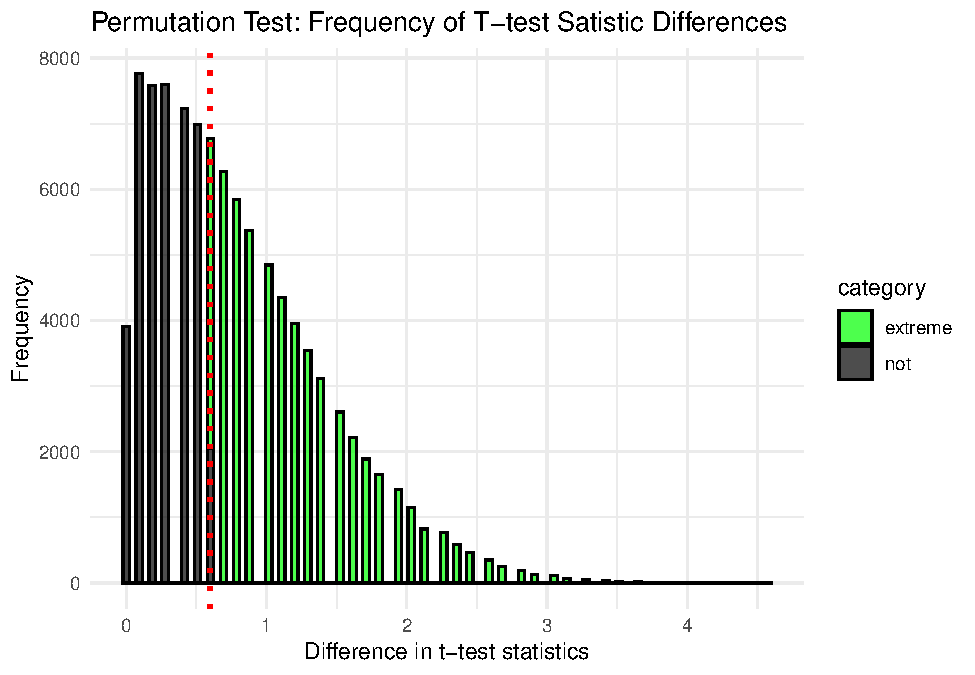
\includegraphics[width=1\linewidth]{lexidate-holdout-supplemental_files/figure-latex/task-146818-test-95-pv-1}

\hypertarget{selection-set-accuracy-4}{%
\subsection{Selection set accuracy}\label{selection-set-accuracy-4}}

\begin{Shaded}
\begin{Highlighting}[]
\FunctionTok{selection\_plot}\NormalTok{(}\FunctionTok{filter}\NormalTok{(task\_data, split }\SpecialCharTok{==} \StringTok{\textquotesingle{}95\%\textquotesingle{}}\NormalTok{))}
\end{Highlighting}
\end{Shaded}

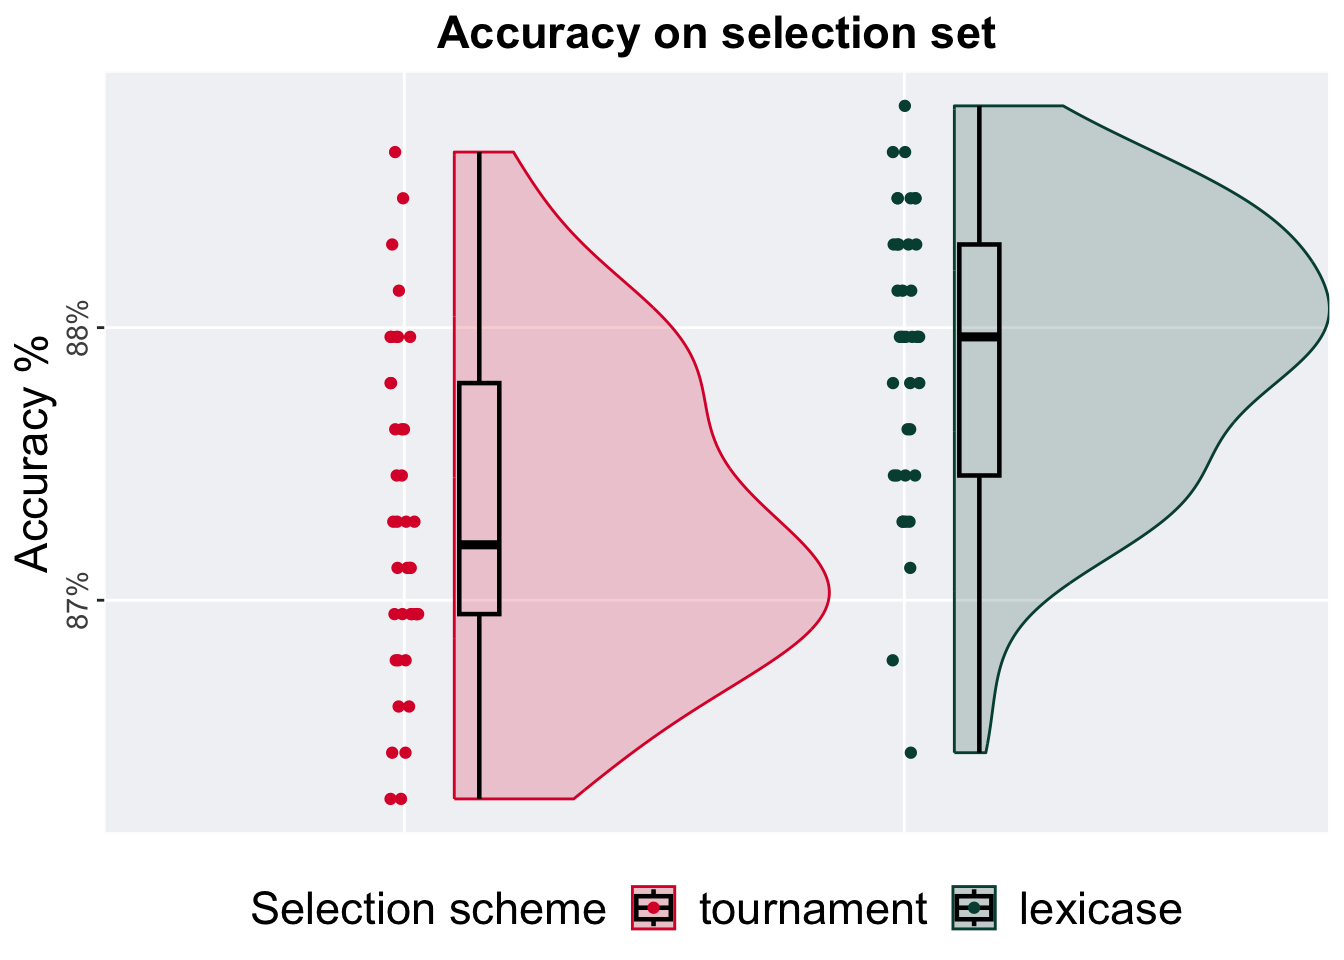
\includegraphics[width=1\linewidth]{lexidate-holdout-supplemental_files/figure-latex/task-146818-select-95-perf-1}

Summary statistics for the testing performance of the selection schemes at the 5\% selection set split:

\begin{Shaded}
\begin{Highlighting}[]
\FunctionTok{selection\_results\_summary}\NormalTok{(}\FunctionTok{filter}\NormalTok{(task\_data, split }\SpecialCharTok{==} \StringTok{\textquotesingle{}95\%\textquotesingle{}}\NormalTok{))}
\end{Highlighting}
\end{Shaded}

\begin{verbatim}
## # A tibble: 2 x 8
##   selection  count na_cnt   min median  mean   max     IQR
##   <fct>      <int>  <int> <dbl>  <dbl> <dbl> <dbl>   <dbl>
## 1 tournament    40      0 0.863  0.872 0.873 0.886 0.00847
## 2 lexicase      40      0 0.864  0.880 0.879 0.888 0.00847
\end{verbatim}

The permutation test revealed that the results are:

\begin{Shaded}
\begin{Highlighting}[]
\NormalTok{tournament\_results }\OtherTok{\textless{}{-}} \FunctionTok{filter}\NormalTok{(task\_data, split }\SpecialCharTok{==} \StringTok{\textquotesingle{}95\%\textquotesingle{}} \SpecialCharTok{\&}\NormalTok{ selection }\SpecialCharTok{==} \StringTok{\textquotesingle{}tournament\textquotesingle{}}\NormalTok{)}
\NormalTok{lexicase\_results }\OtherTok{\textless{}{-}} \FunctionTok{filter}\NormalTok{(task\_data, split }\SpecialCharTok{==} \StringTok{\textquotesingle{}95\%\textquotesingle{}} \SpecialCharTok{\&}\NormalTok{ selection }\SpecialCharTok{==} \StringTok{\textquotesingle{}lexicase\textquotesingle{}}\NormalTok{)}
\FunctionTok{permutation\_test}\NormalTok{(tournament\_results}\SpecialCharTok{$}\NormalTok{training\_performance,}
\NormalTok{                    lexicase\_results}\SpecialCharTok{$}\NormalTok{training\_performance,}
                    \AttributeTok{seed =} \DecValTok{10}\NormalTok{,}
                    \AttributeTok{alternative =} \StringTok{"l"}\NormalTok{)}
\end{Highlighting}
\end{Shaded}

\begin{verbatim}
## [1] "observed_diff: -4.71550186673307"
## [1] "permutation_diffs[0.05 * n_permutations]: -1.6695026702645"
## [1] "reject null hypothesis"
## [1] "p-value: 1e-05"
\end{verbatim}

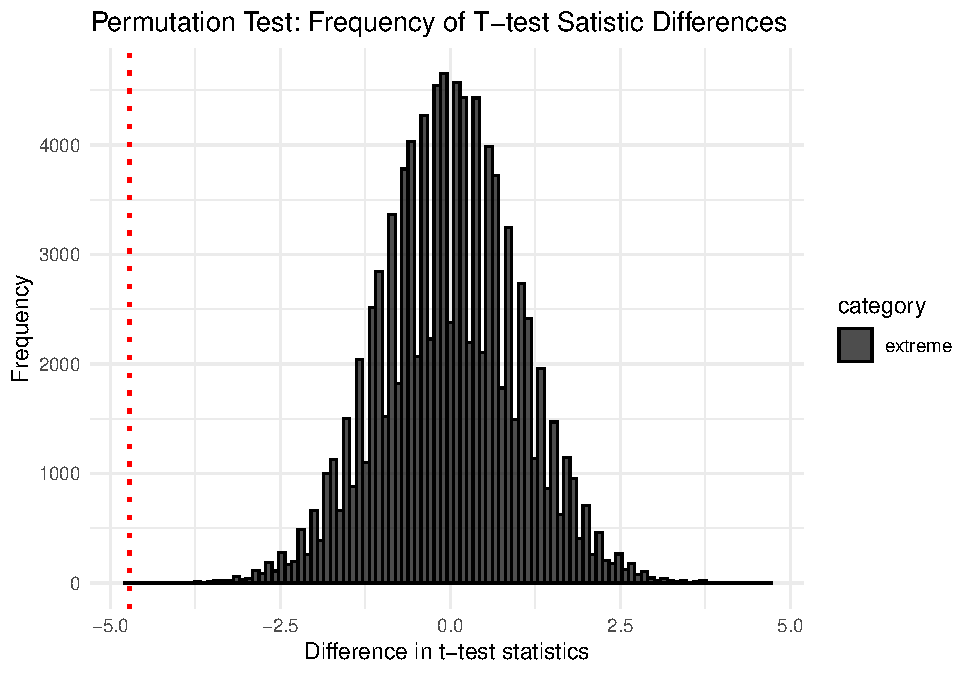
\includegraphics[width=1\linewidth]{lexidate-holdout-supplemental_files/figure-latex/task-146818-select-95-pv-1}

\hypertarget{task-359954}{%
\chapter{Task 359954}\label{task-359954}}

We present the results of our analysis of \texttt{task\ 359954} with the different selection set splits used in our study.

\begin{Shaded}
\begin{Highlighting}[]
\NormalTok{task\_data }\OtherTok{\textless{}{-}} \FunctionTok{filter}\NormalTok{(results, task\_id }\SpecialCharTok{==} \DecValTok{359954}\NormalTok{)}
\end{Highlighting}
\end{Shaded}

\hypertarget{section-5}\label{section-5}}

\hypertarget{testing-set-accuracy-5}{%
\subsection{Testing set accuracy}\label{testing-set-accuracy-5}}

\begin{Shaded}
\begin{Highlighting}[]
\FunctionTok{test\_plot}\NormalTok{(}\FunctionTok{filter}\NormalTok{(task\_data, split }\SpecialCharTok{==} \StringTok{\textquotesingle{}5\%\textquotesingle{}}\NormalTok{))}
\end{Highlighting}
\end{Shaded}

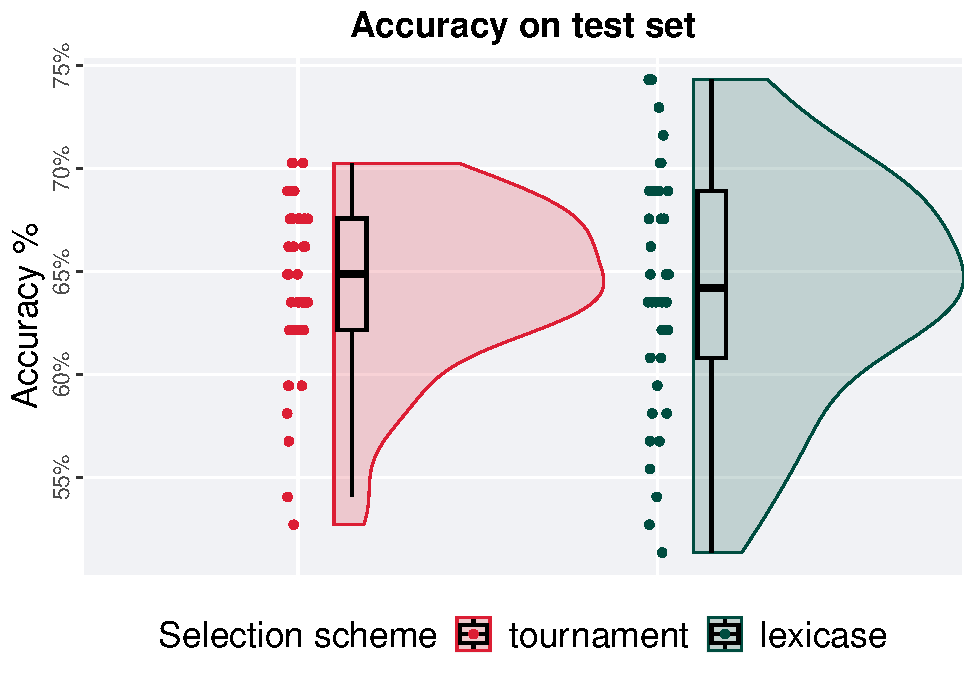
\includegraphics[width=1\linewidth]{lexidate-holdout-supplemental_files/figure-latex/task-359954-test-05-perf-1}

Summary statistics for the testing performance of the selection schemes at the 5\% selection set split:

\begin{Shaded}
\begin{Highlighting}[]
\FunctionTok{test\_results\_summary}\NormalTok{(}\FunctionTok{filter}\NormalTok{(task\_data, split }\SpecialCharTok{==} \StringTok{\textquotesingle{}5\%\textquotesingle{}}\NormalTok{))}
\end{Highlighting}
\end{Shaded}

\begin{verbatim}
## # A tibble: 2 x 8
##   selection  count na_cnt   min median  mean   max    IQR
##   <fct>      <int>  <int> <dbl>  <dbl> <dbl> <dbl>  <dbl>
## 1 tournament    40      0 0.527  0.649 0.643 0.703 0.0541
## 2 lexicase      40      0 0.514  0.642 0.642 0.743 0.0811
\end{verbatim}

The permutation test revealed that the results are:

\begin{Shaded}
\begin{Highlighting}[]
\NormalTok{tournament\_results }\OtherTok{\textless{}{-}} \FunctionTok{filter}\NormalTok{(task\_data, split }\SpecialCharTok{==} \StringTok{\textquotesingle{}5\%\textquotesingle{}} \SpecialCharTok{\&}\NormalTok{ selection }\SpecialCharTok{==} \StringTok{\textquotesingle{}tournament\textquotesingle{}}\NormalTok{)}
\NormalTok{lexicase\_results }\OtherTok{\textless{}{-}} \FunctionTok{filter}\NormalTok{(task\_data, split }\SpecialCharTok{==} \StringTok{\textquotesingle{}5\%\textquotesingle{}} \SpecialCharTok{\&}\NormalTok{ selection }\SpecialCharTok{==} \StringTok{\textquotesingle{}lexicase\textquotesingle{}}\NormalTok{)}
\FunctionTok{permutation\_test}\NormalTok{(tournament\_results}\SpecialCharTok{$}\NormalTok{testing\_performance,}
\NormalTok{                    lexicase\_results}\SpecialCharTok{$}\NormalTok{testing\_performance,}
                    \AttributeTok{seed =} \DecValTok{11}\NormalTok{,}
                    \AttributeTok{alternative =} \StringTok{"t"}\NormalTok{)}
\end{Highlighting}
\end{Shaded}

\begin{verbatim}
## [1] "observed_diff: 0.089899097880169"
## [1] "lower: -1.99686947621326"
## [1] "upper: 1.99686947621326"
## [1] "fail to reject null hypothesis"
## [1] "p-value: 0.91166"
\end{verbatim}

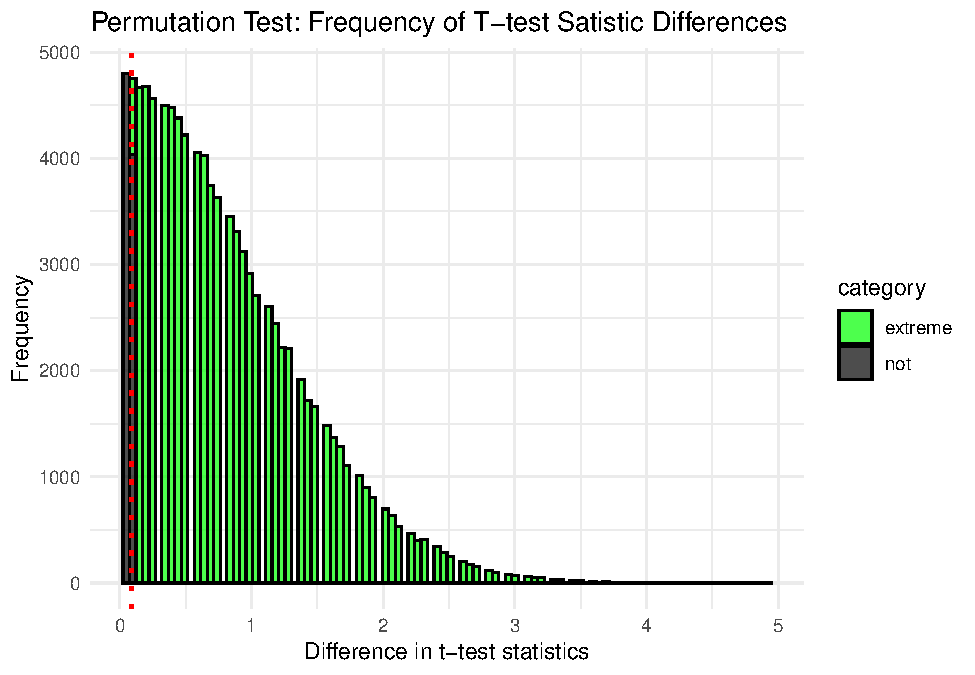
\includegraphics[width=1\linewidth]{lexidate-holdout-supplemental_files/figure-latex/task-359954-test-05-pv-1}

\hypertarget{selection-set-accuracy-5}{%
\subsection{Selection set accuracy}\label{selection-set-accuracy-5}}

\begin{Shaded}
\begin{Highlighting}[]
\FunctionTok{selection\_plot}\NormalTok{(}\FunctionTok{filter}\NormalTok{(task\_data, split }\SpecialCharTok{==} \StringTok{\textquotesingle{}5\%\textquotesingle{}}\NormalTok{))}
\end{Highlighting}
\end{Shaded}

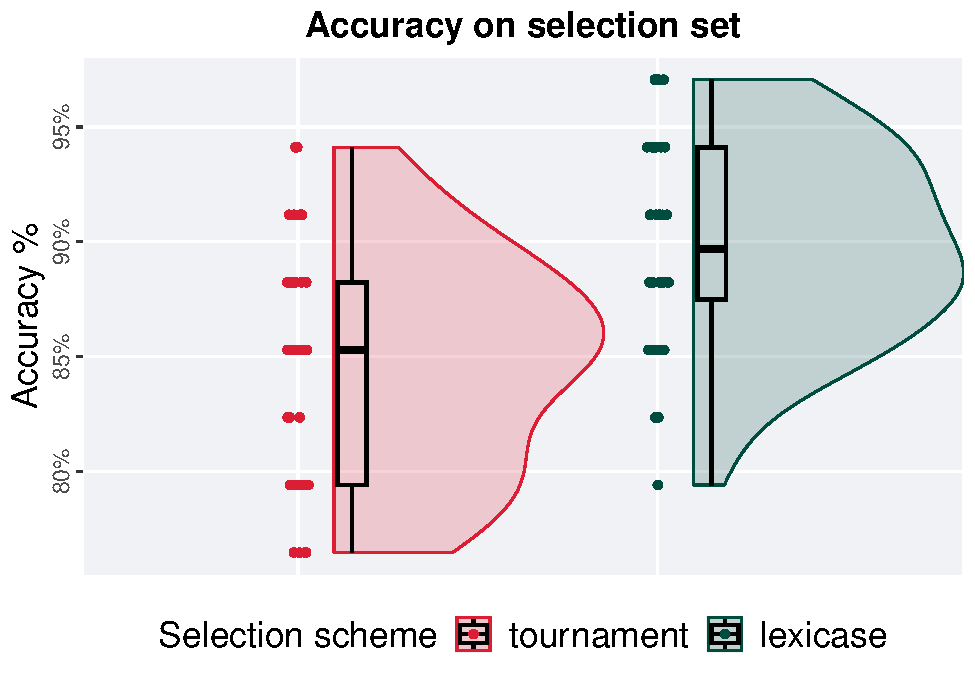
\includegraphics[width=1\linewidth]{lexidate-holdout-supplemental_files/figure-latex/task-359954-select-05-perf-1}

Summary statistics for the testing performance of the selection schemes at the 5\% selection set split:

\begin{Shaded}
\begin{Highlighting}[]
\FunctionTok{selection\_results\_summary}\NormalTok{(}\FunctionTok{filter}\NormalTok{(task\_data, split }\SpecialCharTok{==} \StringTok{\textquotesingle{}5\%\textquotesingle{}}\NormalTok{))}
\end{Highlighting}
\end{Shaded}

\begin{verbatim}
## # A tibble: 2 x 8
##   selection  count na_cnt   min median  mean   max    IQR
##   <fct>      <int>  <int> <dbl>  <dbl> <dbl> <dbl>  <dbl>
## 1 tournament    40      0 0.765  0.853 0.846 0.941 0.0882
## 2 lexicase      40      0 0.794  0.897 0.899 0.971 0.0662
\end{verbatim}

The permutation test revealed that the results are:

\begin{Shaded}
\begin{Highlighting}[]
\NormalTok{tournament\_results }\OtherTok{\textless{}{-}} \FunctionTok{filter}\NormalTok{(task\_data, split }\SpecialCharTok{==} \StringTok{\textquotesingle{}5\%\textquotesingle{}} \SpecialCharTok{\&}\NormalTok{ selection }\SpecialCharTok{==} \StringTok{\textquotesingle{}tournament\textquotesingle{}}\NormalTok{)}
\NormalTok{lexicase\_results }\OtherTok{\textless{}{-}} \FunctionTok{filter}\NormalTok{(task\_data, split }\SpecialCharTok{==} \StringTok{\textquotesingle{}5\%\textquotesingle{}} \SpecialCharTok{\&}\NormalTok{ selection }\SpecialCharTok{==} \StringTok{\textquotesingle{}lexicase\textquotesingle{}}\NormalTok{)}
\FunctionTok{permutation\_test}\NormalTok{(tournament\_results}\SpecialCharTok{$}\NormalTok{training\_performance,}
\NormalTok{                    lexicase\_results}\SpecialCharTok{$}\NormalTok{training\_performance,}
                    \AttributeTok{seed =} \DecValTok{12}\NormalTok{,}
                    \AttributeTok{alternative =} \StringTok{"l"}\NormalTok{)}
\end{Highlighting}
\end{Shaded}

\begin{verbatim}
## [1] "observed_diff: -4.99649396670713"
## [1] "permutation_diffs[0.05 * n_permutations]: -1.68354186553216"
## [1] "reject null hypothesis"
## [1] "p-value: 1e-05"
\end{verbatim}

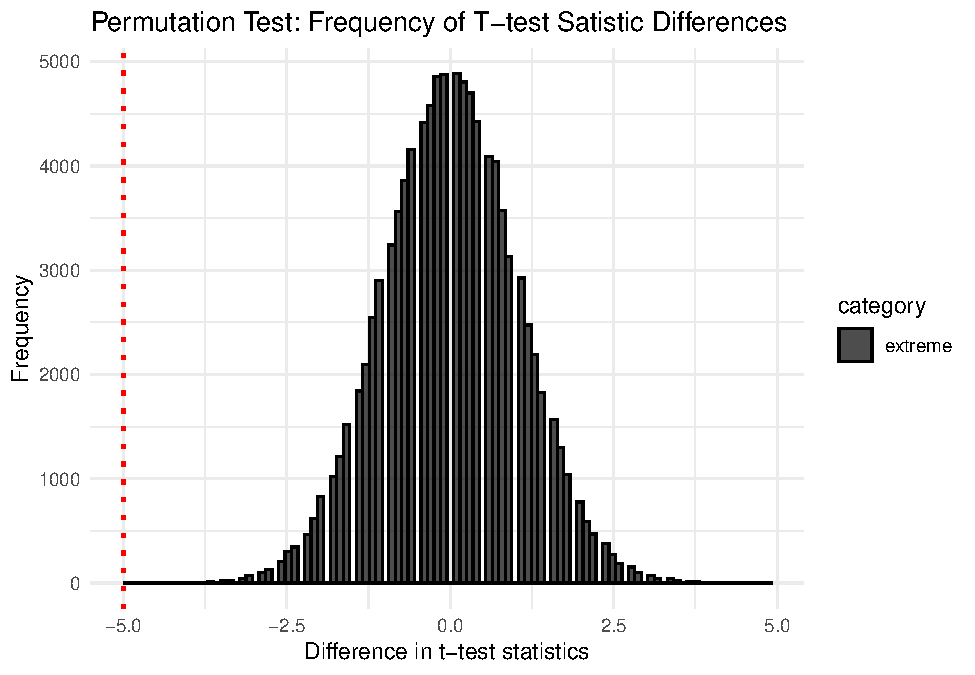
\includegraphics[width=1\linewidth]{lexidate-holdout-supplemental_files/figure-latex/task-359954-select-05-pv-1}

\hypertarget{section-6}\label{section-6}}

\hypertarget{testing-set-accuracy-6}{%
\subsection{Testing set accuracy}\label{testing-set-accuracy-6}}

\begin{Shaded}
\begin{Highlighting}[]
\FunctionTok{test\_plot}\NormalTok{(}\FunctionTok{filter}\NormalTok{(task\_data, split }\SpecialCharTok{==} \StringTok{\textquotesingle{}10\%\textquotesingle{}}\NormalTok{))}
\end{Highlighting}
\end{Shaded}

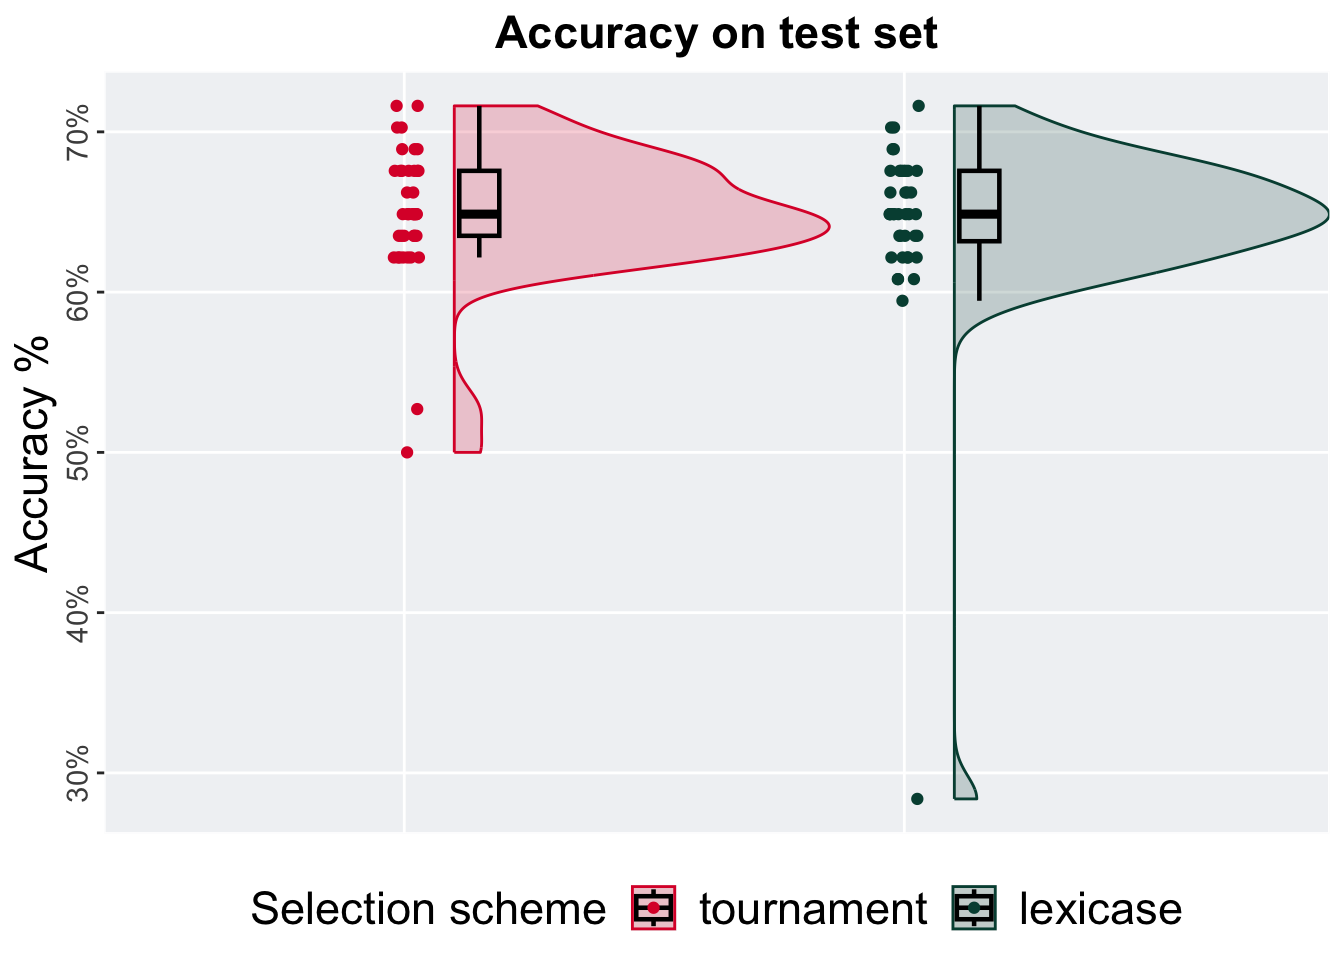
\includegraphics[width=1\linewidth]{lexidate-holdout-supplemental_files/figure-latex/task-359954-test-10-perf-1}

Summary statistics for the testing performance of the selection schemes at the 5\% selection set split:

\begin{Shaded}
\begin{Highlighting}[]
\FunctionTok{test\_results\_summary}\NormalTok{(}\FunctionTok{filter}\NormalTok{(task\_data, split }\SpecialCharTok{==} \StringTok{\textquotesingle{}10\%\textquotesingle{}}\NormalTok{))}
\end{Highlighting}
\end{Shaded}

\begin{verbatim}
## # A tibble: 2 x 8
##   selection  count na_cnt   min median  mean   max    IQR
##   <fct>      <int>  <int> <dbl>  <dbl> <dbl> <dbl>  <dbl>
## 1 tournament    40      0 0.5    0.649 0.650 0.716 0.0405
## 2 lexicase      40      0 0.284  0.649 0.643 0.716 0.0439
\end{verbatim}

The permutation test revealed that the results are:

\begin{Shaded}
\begin{Highlighting}[]
\NormalTok{tournament\_results }\OtherTok{\textless{}{-}} \FunctionTok{filter}\NormalTok{(task\_data, split }\SpecialCharTok{==} \StringTok{\textquotesingle{}10\%\textquotesingle{}} \SpecialCharTok{\&}\NormalTok{ selection }\SpecialCharTok{==} \StringTok{\textquotesingle{}tournament\textquotesingle{}}\NormalTok{)}
\NormalTok{lexicase\_results }\OtherTok{\textless{}{-}} \FunctionTok{filter}\NormalTok{(task\_data, split }\SpecialCharTok{==} \StringTok{\textquotesingle{}10\%\textquotesingle{}} \SpecialCharTok{\&}\NormalTok{ selection }\SpecialCharTok{==} \StringTok{\textquotesingle{}lexicase\textquotesingle{}}\NormalTok{)}
\FunctionTok{permutation\_test}\NormalTok{(tournament\_results}\SpecialCharTok{$}\NormalTok{testing\_performance,}
\NormalTok{                    lexicase\_results}\SpecialCharTok{$}\NormalTok{testing\_performance,}
                    \AttributeTok{seed =} \DecValTok{13}\NormalTok{,}
                    \AttributeTok{alternative =} \StringTok{"t"}\NormalTok{)}
\end{Highlighting}
\end{Shaded}

\begin{verbatim}
## [1] "observed_diff: 0.581706669215585"
## [1] "lower: -1.89401584174984"
## [1] "upper: 1.89401627937136"
## [1] "fail to reject null hypothesis"
## [1] "p-value: 0.63091"
\end{verbatim}

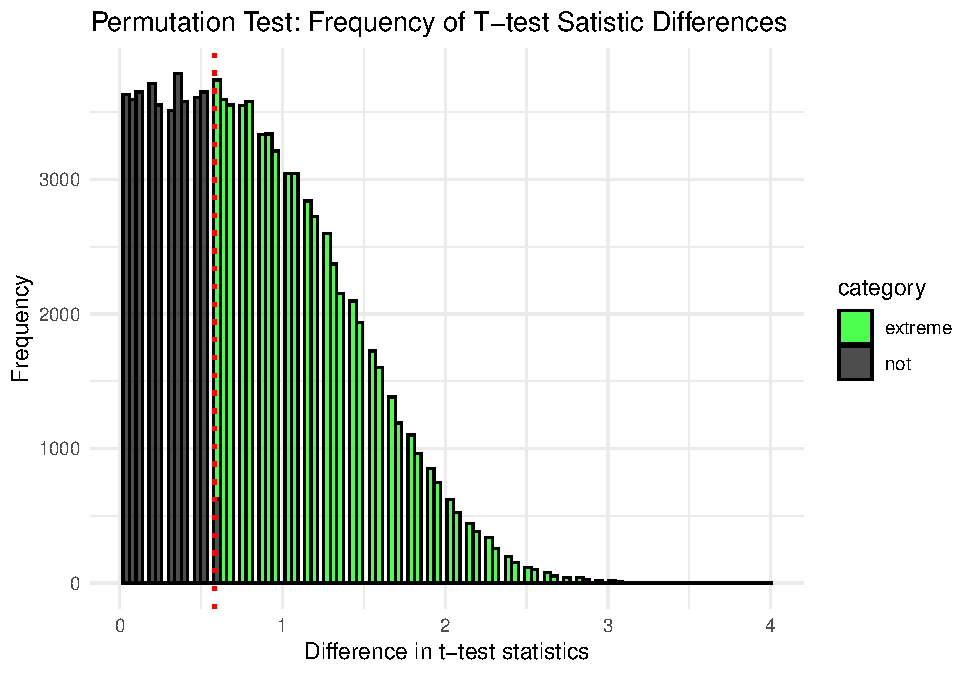
\includegraphics[width=1\linewidth]{lexidate-holdout-supplemental_files/figure-latex/task-359954-test-10-pv-1}

\hypertarget{selection-set-accuracy-6}{%
\subsection{Selection set accuracy}\label{selection-set-accuracy-6}}

\begin{Shaded}
\begin{Highlighting}[]
\FunctionTok{selection\_plot}\NormalTok{(}\FunctionTok{filter}\NormalTok{(task\_data, split }\SpecialCharTok{==} \StringTok{\textquotesingle{}10\%\textquotesingle{}}\NormalTok{))}
\end{Highlighting}
\end{Shaded}

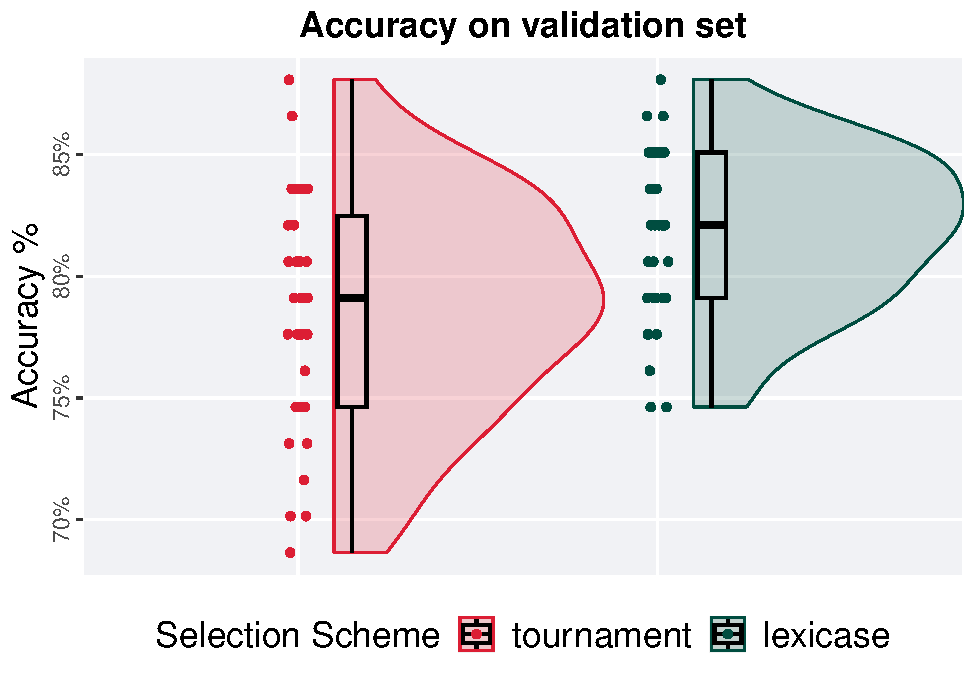
\includegraphics[width=1\linewidth]{lexidate-holdout-supplemental_files/figure-latex/task-359954-select-10-perf-1}

Summary statistics for the testing performance of the selection schemes at the 5\% selection set split:

\begin{Shaded}
\begin{Highlighting}[]
\FunctionTok{selection\_results\_summary}\NormalTok{(}\FunctionTok{filter}\NormalTok{(task\_data, split }\SpecialCharTok{==} \StringTok{\textquotesingle{}10\%\textquotesingle{}}\NormalTok{))}
\end{Highlighting}
\end{Shaded}

\begin{verbatim}
## # A tibble: 2 x 8
##   selection  count na_cnt   min median  mean   max    IQR
##   <fct>      <int>  <int> <dbl>  <dbl> <dbl> <dbl>  <dbl>
## 1 tournament    40      0 0.687  0.791 0.787 0.881 0.0784
## 2 lexicase      40      0 0.746  0.821 0.818 0.881 0.0597
\end{verbatim}

The permutation test revealed that the results are:

\begin{Shaded}
\begin{Highlighting}[]
\NormalTok{tournament\_results }\OtherTok{\textless{}{-}} \FunctionTok{filter}\NormalTok{(task\_data, split }\SpecialCharTok{==} \StringTok{\textquotesingle{}10\%\textquotesingle{}} \SpecialCharTok{\&}\NormalTok{ selection }\SpecialCharTok{==} \StringTok{\textquotesingle{}tournament\textquotesingle{}}\NormalTok{)}
\NormalTok{lexicase\_results }\OtherTok{\textless{}{-}} \FunctionTok{filter}\NormalTok{(task\_data, split }\SpecialCharTok{==} \StringTok{\textquotesingle{}10\%\textquotesingle{}} \SpecialCharTok{\&}\NormalTok{ selection }\SpecialCharTok{==} \StringTok{\textquotesingle{}lexicase\textquotesingle{}}\NormalTok{)}
\FunctionTok{permutation\_test}\NormalTok{(tournament\_results}\SpecialCharTok{$}\NormalTok{training\_performance,}
\NormalTok{                    lexicase\_results}\SpecialCharTok{$}\NormalTok{training\_performance,}
                    \AttributeTok{seed =} \DecValTok{14}\NormalTok{,}
                    \AttributeTok{alternative =} \StringTok{"l"}\NormalTok{)}
\end{Highlighting}
\end{Shaded}

\begin{verbatim}
## [1] "observed_diff: -3.49007120627971"
## [1] "permutation_diffs[0.05 * n_permutations]: -1.65102702194372"
## [1] "reject null hypothesis"
## [1] "p-value: 0.00027"
\end{verbatim}

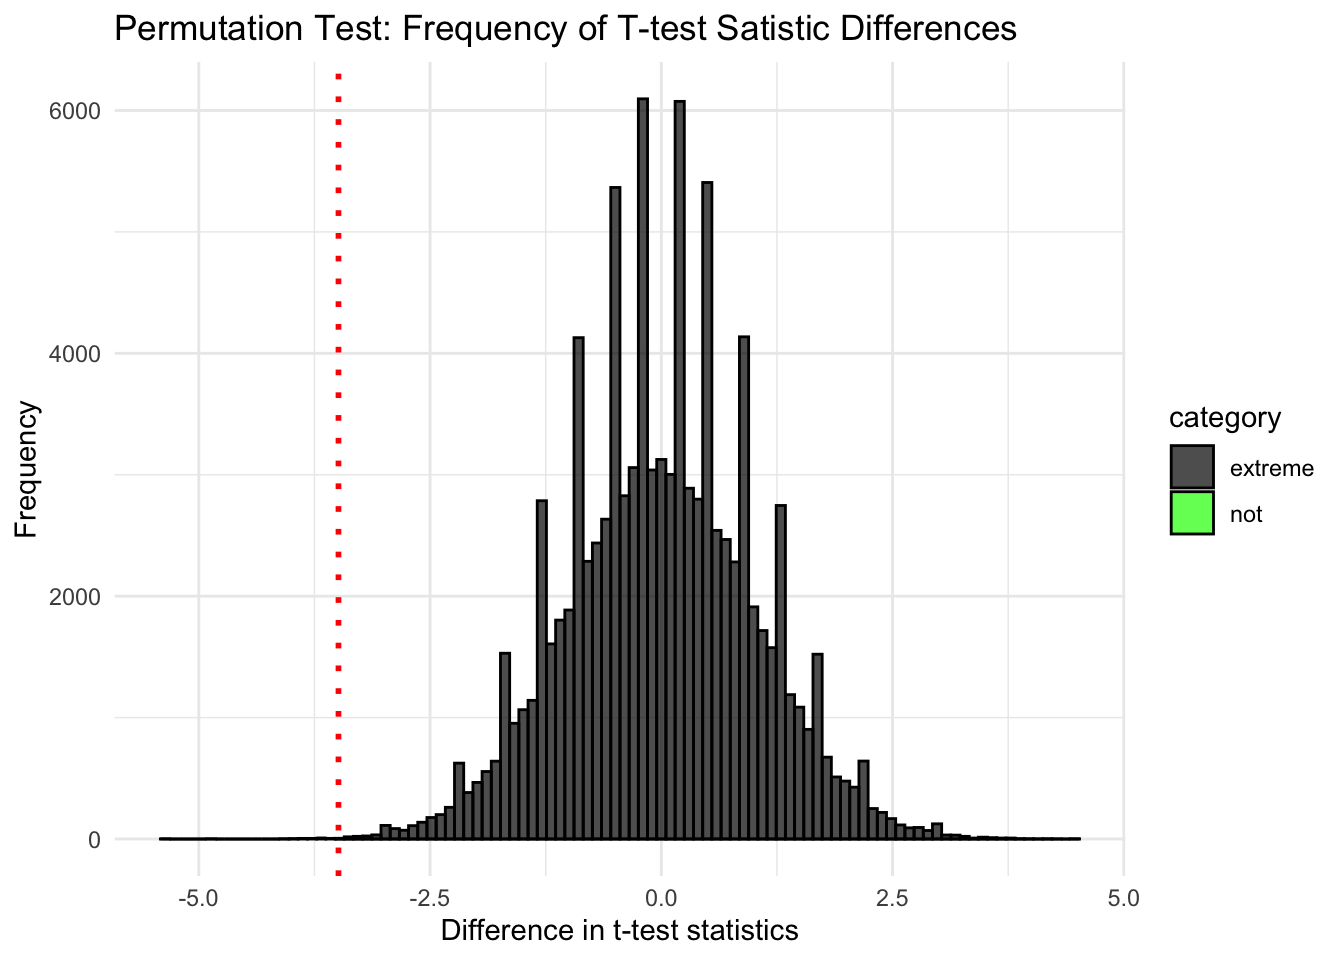
\includegraphics[width=1\linewidth]{lexidate-holdout-supplemental_files/figure-latex/task-359954-select-10-pv-1}

\hypertarget{section-7}\label{section-7}}

\hypertarget{testing-set-accuracy-7}{%
\subsection{Testing set accuracy}\label{testing-set-accuracy-7}}

\begin{Shaded}
\begin{Highlighting}[]
\FunctionTok{test\_plot}\NormalTok{(}\FunctionTok{filter}\NormalTok{(task\_data, split }\SpecialCharTok{==} \StringTok{\textquotesingle{}50\%\textquotesingle{}}\NormalTok{))}
\end{Highlighting}
\end{Shaded}

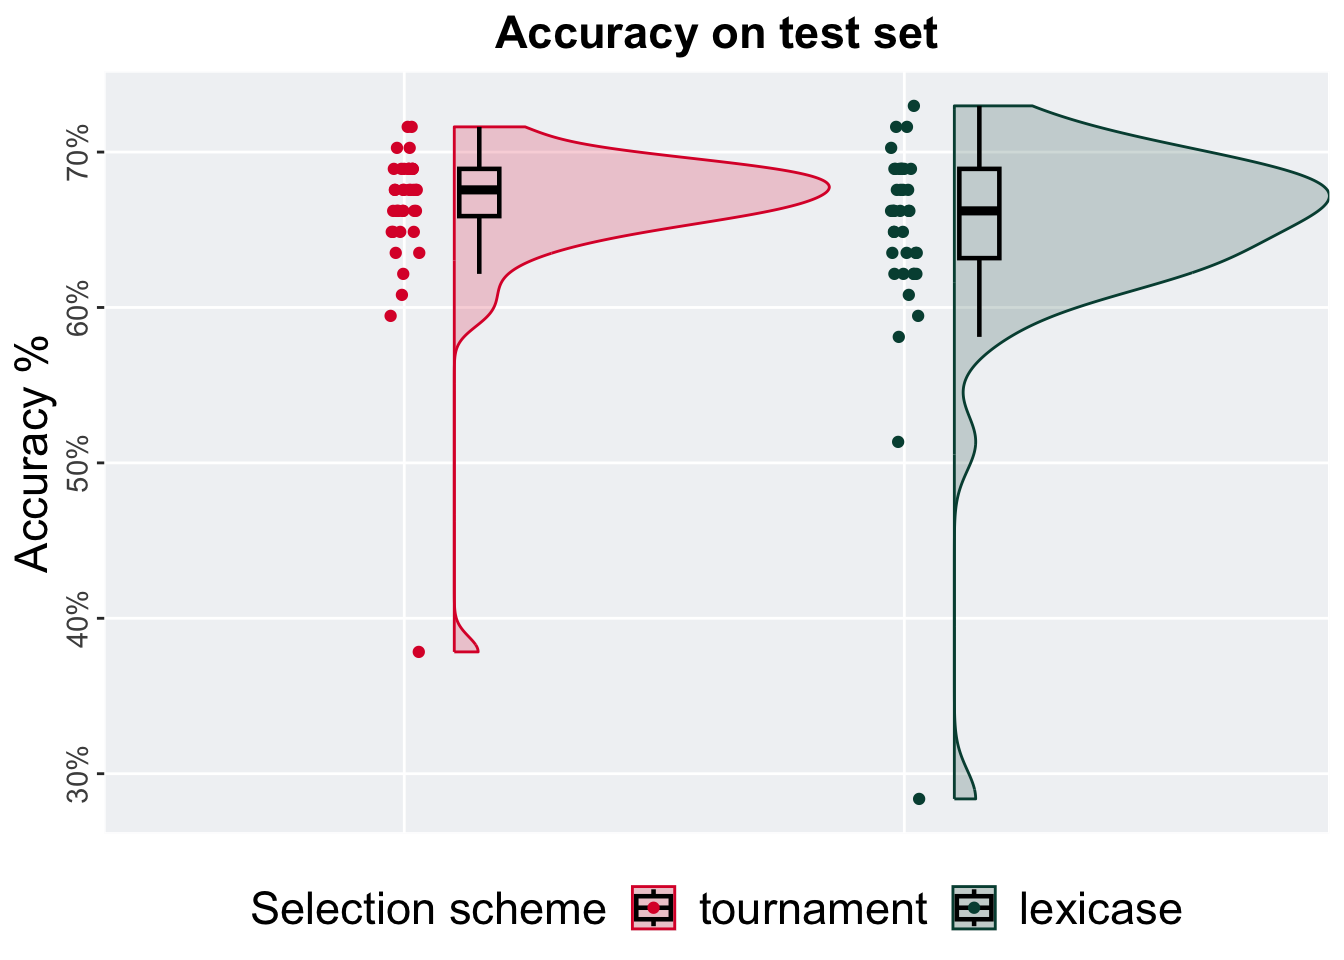
\includegraphics[width=1\linewidth]{lexidate-holdout-supplemental_files/figure-latex/task-359954-test-50-perf-1}

Summary statistics for the testing performance of the selection schemes at the 5\% selection set split:

\begin{Shaded}
\begin{Highlighting}[]
\FunctionTok{test\_results\_summary}\NormalTok{(}\FunctionTok{filter}\NormalTok{(task\_data, split }\SpecialCharTok{==} \StringTok{\textquotesingle{}50\%\textquotesingle{}}\NormalTok{))}
\end{Highlighting}
\end{Shaded}

\begin{verbatim}
## # A tibble: 2 x 8
##   selection  count na_cnt   min median  mean   max    IQR
##   <fct>      <int>  <int> <dbl>  <dbl> <dbl> <dbl>  <dbl>
## 1 tournament    40      0 0.378  0.676 0.662 0.716 0.0304
## 2 lexicase      40      0 0.284  0.662 0.647 0.730 0.0574
\end{verbatim}

The permutation test revealed that the results are:

\begin{Shaded}
\begin{Highlighting}[]
\NormalTok{tournament\_results }\OtherTok{\textless{}{-}} \FunctionTok{filter}\NormalTok{(task\_data, split }\SpecialCharTok{==} \StringTok{\textquotesingle{}50\%\textquotesingle{}} \SpecialCharTok{\&}\NormalTok{ selection }\SpecialCharTok{==} \StringTok{\textquotesingle{}tournament\textquotesingle{}}\NormalTok{)}
\NormalTok{lexicase\_results }\OtherTok{\textless{}{-}} \FunctionTok{filter}\NormalTok{(task\_data, split }\SpecialCharTok{==} \StringTok{\textquotesingle{}50\%\textquotesingle{}} \SpecialCharTok{\&}\NormalTok{ selection }\SpecialCharTok{==} \StringTok{\textquotesingle{}lexicase\textquotesingle{}}\NormalTok{)}
\FunctionTok{permutation\_test}\NormalTok{(tournament\_results}\SpecialCharTok{$}\NormalTok{testing\_performance,}
\NormalTok{                    lexicase\_results}\SpecialCharTok{$}\NormalTok{testing\_performance,}
                    \AttributeTok{seed =} \DecValTok{15}\NormalTok{,}
                    \AttributeTok{alternative =} \StringTok{"t"}\NormalTok{)}
\end{Highlighting}
\end{Shaded}

\begin{verbatim}
## [1] "observed_diff: 1.05447797672778"
## [1] "lower: -1.89851953697627"
## [1] "upper: 1.89851953697627"
## [1] "fail to reject null hypothesis"
## [1] "p-value: 0.31566"
\end{verbatim}

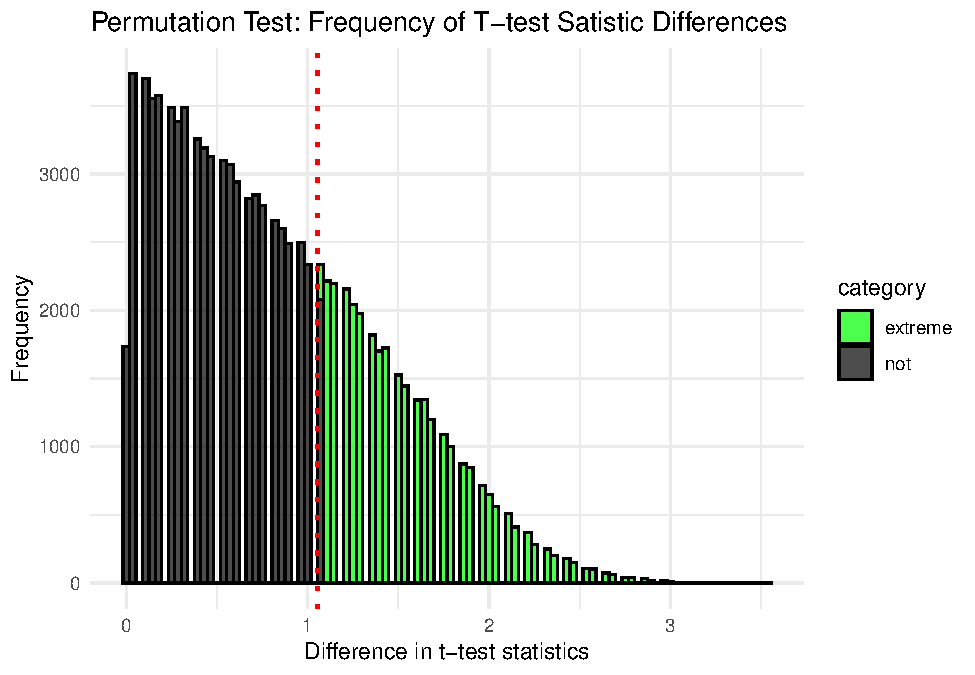
\includegraphics[width=1\linewidth]{lexidate-holdout-supplemental_files/figure-latex/task-359954-test-50-pv-1}

\hypertarget{selection-set-accuracy-7}{%
\subsection{Selection set accuracy}\label{selection-set-accuracy-7}}

\begin{Shaded}
\begin{Highlighting}[]
\FunctionTok{selection\_plot}\NormalTok{(}\FunctionTok{filter}\NormalTok{(task\_data, split }\SpecialCharTok{==} \StringTok{\textquotesingle{}50\%\textquotesingle{}}\NormalTok{))}
\end{Highlighting}
\end{Shaded}

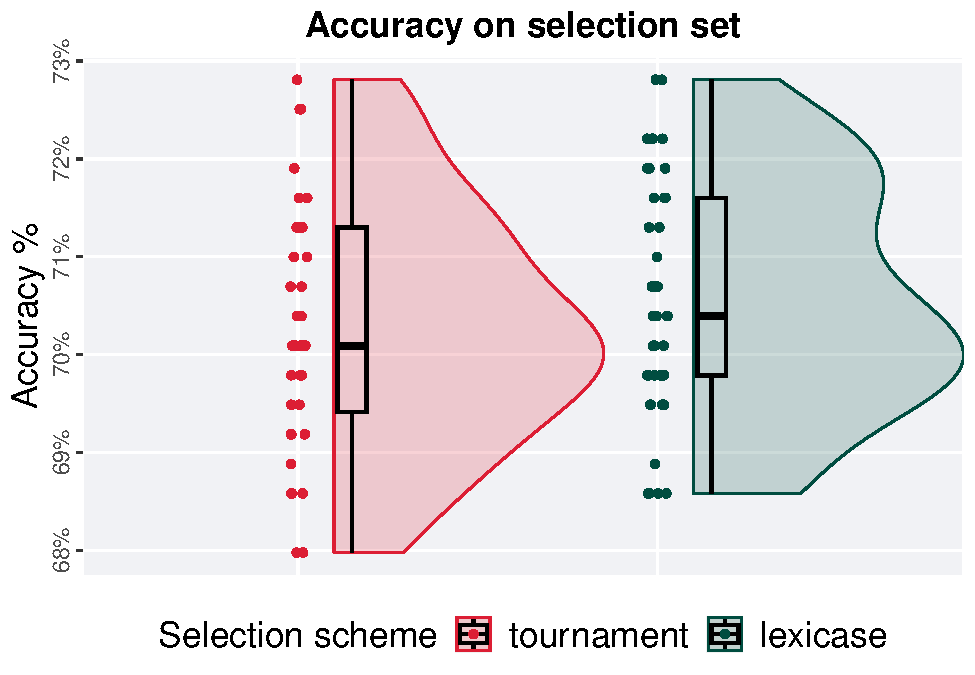
\includegraphics[width=1\linewidth]{lexidate-holdout-supplemental_files/figure-latex/task-359954-select-50-perf-1}

Summary statistics for the testing performance of the selection schemes at the 5\% selection set split:

\begin{Shaded}
\begin{Highlighting}[]
\FunctionTok{selection\_results\_summary}\NormalTok{(}\FunctionTok{filter}\NormalTok{(task\_data, split }\SpecialCharTok{==} \StringTok{\textquotesingle{}50\%\textquotesingle{}}\NormalTok{))}
\end{Highlighting}
\end{Shaded}

\begin{verbatim}
## # A tibble: 2 x 8
##   selection  count na_cnt   min median  mean   max    IQR
##   <fct>      <int>  <int> <dbl>  <dbl> <dbl> <dbl>  <dbl>
## 1 tournament    40      0 0.680  0.701 0.703 0.728 0.0189
## 2 lexicase      40      0 0.686  0.704 0.706 0.728 0.0181
\end{verbatim}

The permutation test revealed that the results are:

\begin{Shaded}
\begin{Highlighting}[]
\NormalTok{tournament\_results }\OtherTok{\textless{}{-}} \FunctionTok{filter}\NormalTok{(task\_data, split }\SpecialCharTok{==} \StringTok{\textquotesingle{}50\%\textquotesingle{}} \SpecialCharTok{\&}\NormalTok{ selection }\SpecialCharTok{==} \StringTok{\textquotesingle{}tournament\textquotesingle{}}\NormalTok{)}
\NormalTok{lexicase\_results }\OtherTok{\textless{}{-}} \FunctionTok{filter}\NormalTok{(task\_data, split }\SpecialCharTok{==} \StringTok{\textquotesingle{}50\%\textquotesingle{}} \SpecialCharTok{\&}\NormalTok{ selection }\SpecialCharTok{==} \StringTok{\textquotesingle{}lexicase\textquotesingle{}}\NormalTok{)}
\FunctionTok{permutation\_test}\NormalTok{(tournament\_results}\SpecialCharTok{$}\NormalTok{training\_performance,}
\NormalTok{                    lexicase\_results}\SpecialCharTok{$}\NormalTok{training\_performance,}
                    \AttributeTok{seed =} \DecValTok{16}\NormalTok{,}
                    \AttributeTok{alternative =} \StringTok{"t"}\NormalTok{)}
\end{Highlighting}
\end{Shaded}

\begin{verbatim}
## [1] "observed_diff: -1.0089201210214"
## [1] "lower: -1.97083964694619"
## [1] "upper: 1.9708394540355"
## [1] "fail to reject null hypothesis"
## [1] "p-value: 0.32044"
\end{verbatim}

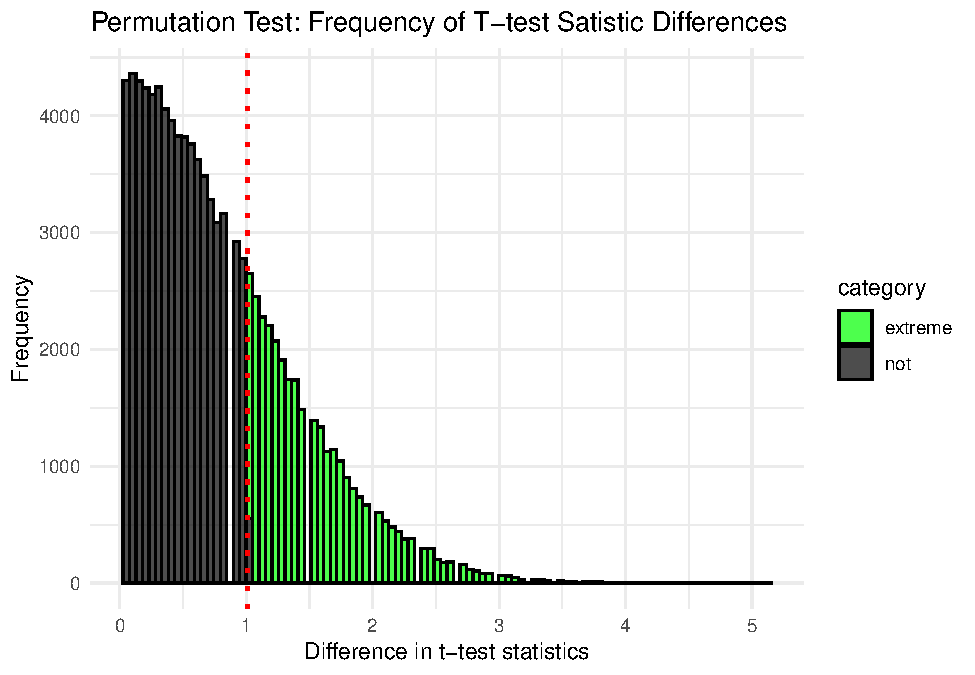
\includegraphics[width=1\linewidth]{lexidate-holdout-supplemental_files/figure-latex/task-359954-select-50-pv-1}

\hypertarget{section-8}\label{section-8}}

\hypertarget{testing-set-accuracy-8}{%
\subsection{Testing set accuracy}\label{testing-set-accuracy-8}}

\begin{Shaded}
\begin{Highlighting}[]
\FunctionTok{test\_plot}\NormalTok{(}\FunctionTok{filter}\NormalTok{(task\_data, split }\SpecialCharTok{==} \StringTok{\textquotesingle{}90\%\textquotesingle{}}\NormalTok{))}
\end{Highlighting}
\end{Shaded}

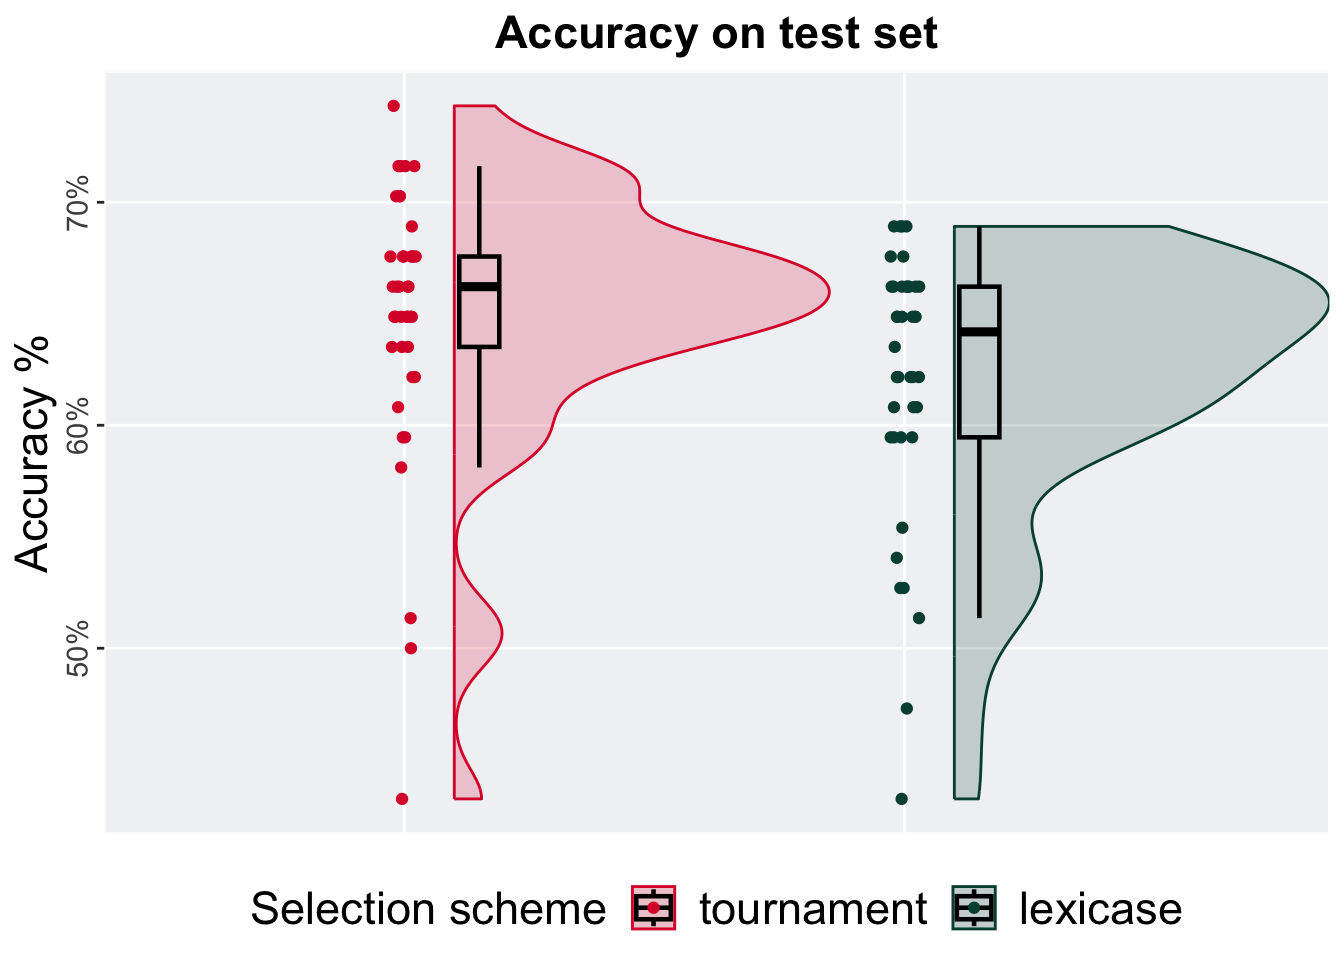
\includegraphics[width=1\linewidth]{lexidate-holdout-supplemental_files/figure-latex/task-359954-test-90-perf-1}

Summary statistics for the testing performance of the selection schemes at the 5\% selection set split:

\begin{Shaded}
\begin{Highlighting}[]
\FunctionTok{test\_results\_summary}\NormalTok{(}\FunctionTok{filter}\NormalTok{(task\_data, split }\SpecialCharTok{==} \StringTok{\textquotesingle{}90\%\textquotesingle{}}\NormalTok{))}
\end{Highlighting}
\end{Shaded}

\begin{verbatim}
## # A tibble: 2 x 8
##   selection  count na_cnt   min median  mean   max    IQR
##   <fct>      <int>  <int> <dbl>  <dbl> <dbl> <dbl>  <dbl>
## 1 tournament    40      0 0.432  0.662 0.649 0.743 0.0405
## 2 lexicase      40      0 0.432  0.642 0.620 0.689 0.0676
\end{verbatim}

The permutation test revealed that the results are:

\begin{Shaded}
\begin{Highlighting}[]
\NormalTok{tournament\_results }\OtherTok{\textless{}{-}} \FunctionTok{filter}\NormalTok{(task\_data, split }\SpecialCharTok{==} \StringTok{\textquotesingle{}90\%\textquotesingle{}} \SpecialCharTok{\&}\NormalTok{ selection }\SpecialCharTok{==} \StringTok{\textquotesingle{}tournament\textquotesingle{}}\NormalTok{)}
\NormalTok{lexicase\_results }\OtherTok{\textless{}{-}} \FunctionTok{filter}\NormalTok{(task\_data, split }\SpecialCharTok{==} \StringTok{\textquotesingle{}90\%\textquotesingle{}} \SpecialCharTok{\&}\NormalTok{ selection }\SpecialCharTok{==} \StringTok{\textquotesingle{}lexicase\textquotesingle{}}\NormalTok{)}
\FunctionTok{permutation\_test}\NormalTok{(tournament\_results}\SpecialCharTok{$}\NormalTok{testing\_performance,}
\NormalTok{                    lexicase\_results}\SpecialCharTok{$}\NormalTok{testing\_performance,}
                    \AttributeTok{seed =} \DecValTok{17}\NormalTok{,}
                    \AttributeTok{alternative =} \StringTok{"g"}\NormalTok{)}
\end{Highlighting}
\end{Shaded}

\begin{verbatim}
## [1] "observed_diff: 2.11112337167441"
## [1] "permutation_diffs[0.95 * n_permutations]: 1.64634620519505"
## [1] "reject null hypothesis"
## [1] "p-value: 0.01917"
\end{verbatim}

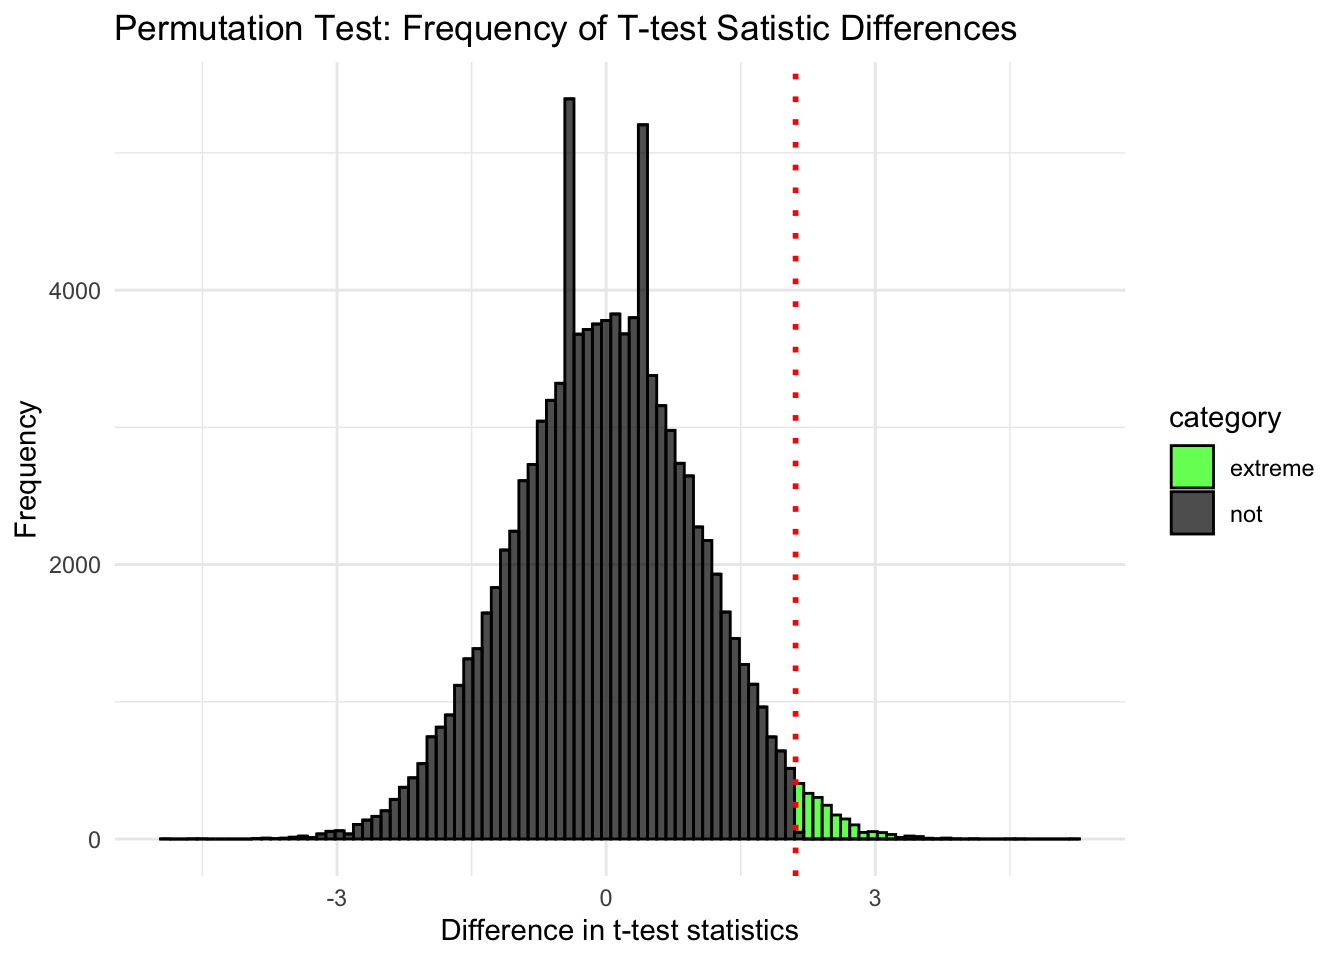
\includegraphics[width=1\linewidth]{lexidate-holdout-supplemental_files/figure-latex/task-359954-test-90-pv-1}

\hypertarget{selection-set-accuracy-8}{%
\subsection{Selection set accuracy}\label{selection-set-accuracy-8}}

\begin{Shaded}
\begin{Highlighting}[]
\FunctionTok{selection\_plot}\NormalTok{(}\FunctionTok{filter}\NormalTok{(task\_data, split }\SpecialCharTok{==} \StringTok{\textquotesingle{}90\%\textquotesingle{}}\NormalTok{))}
\end{Highlighting}
\end{Shaded}

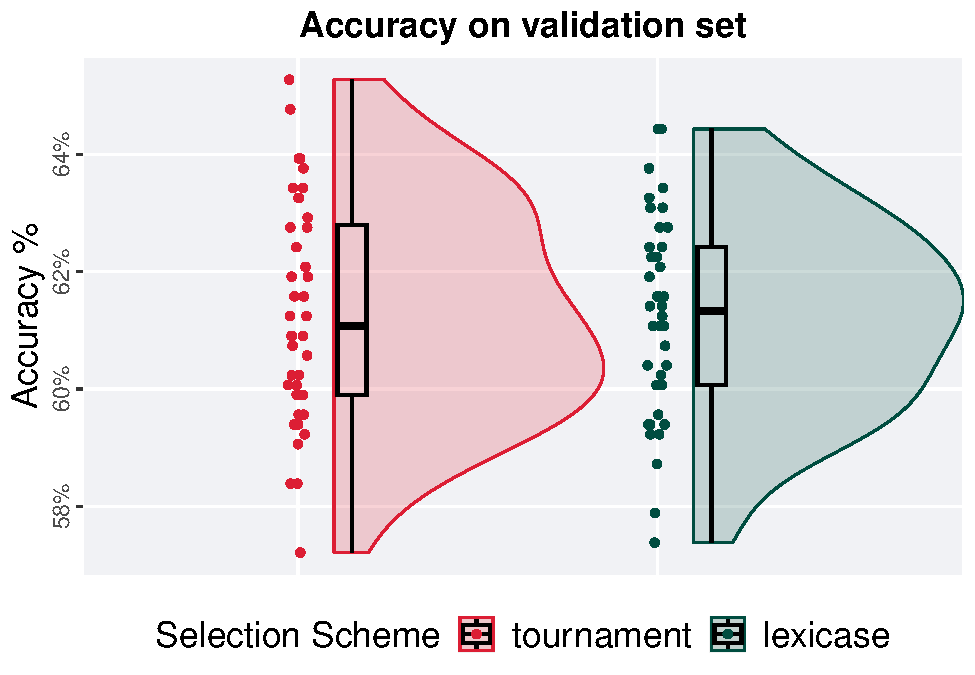
\includegraphics[width=1\linewidth]{lexidate-holdout-supplemental_files/figure-latex/task-359954-select-90-perf-1}

Summary statistics for the testing performance of the selection schemes at the 5\% selection set split:

\begin{Shaded}
\begin{Highlighting}[]
\FunctionTok{selection\_results\_summary}\NormalTok{(}\FunctionTok{filter}\NormalTok{(task\_data, split }\SpecialCharTok{==} \StringTok{\textquotesingle{}90\%\textquotesingle{}}\NormalTok{))}
\end{Highlighting}
\end{Shaded}

\begin{verbatim}
## # A tibble: 2 x 8
##   selection  count na_cnt   min median  mean   max    IQR
##   <fct>      <int>  <int> <dbl>  <dbl> <dbl> <dbl>  <dbl>
## 1 tournament    40      0 0.572  0.611 0.613 0.653 0.0289
## 2 lexicase      40      0 0.574  0.613 0.612 0.644 0.0235
\end{verbatim}

The permutation test revealed that the results are:

\begin{Shaded}
\begin{Highlighting}[]
\NormalTok{tournament\_results }\OtherTok{\textless{}{-}} \FunctionTok{filter}\NormalTok{(task\_data, split }\SpecialCharTok{==} \StringTok{\textquotesingle{}90\%\textquotesingle{}} \SpecialCharTok{\&}\NormalTok{ selection }\SpecialCharTok{==} \StringTok{\textquotesingle{}tournament\textquotesingle{}}\NormalTok{)}
\NormalTok{lexicase\_results }\OtherTok{\textless{}{-}} \FunctionTok{filter}\NormalTok{(task\_data, split }\SpecialCharTok{==} \StringTok{\textquotesingle{}90\%\textquotesingle{}} \SpecialCharTok{\&}\NormalTok{ selection }\SpecialCharTok{==} \StringTok{\textquotesingle{}lexicase\textquotesingle{}}\NormalTok{)}
\FunctionTok{permutation\_test}\NormalTok{(tournament\_results}\SpecialCharTok{$}\NormalTok{training\_performance,}
\NormalTok{                    lexicase\_results}\SpecialCharTok{$}\NormalTok{training\_performance,}
                    \AttributeTok{seed =} \DecValTok{18}\NormalTok{,}
                    \AttributeTok{alternative =} \StringTok{"t"}\NormalTok{)}
\end{Highlighting}
\end{Shaded}

\begin{verbatim}
## [1] "observed_diff: 0.218175712374656"
## [1] "lower: -1.99095942630688"
## [1] "upper: 1.99096129334562"
## [1] "fail to reject null hypothesis"
## [1] "p-value: 0.83358"
\end{verbatim}

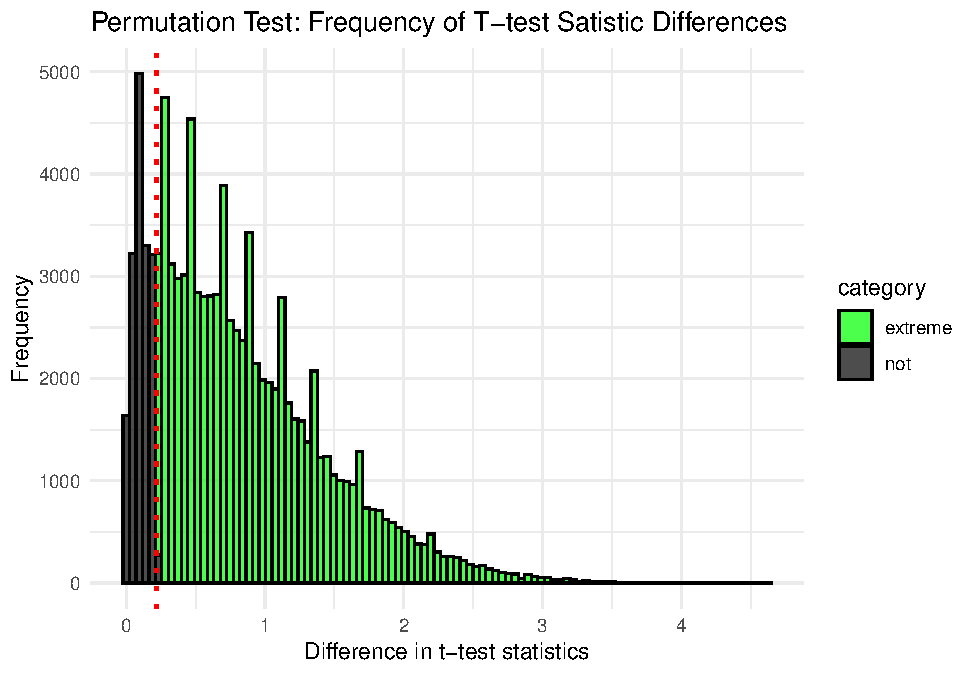
\includegraphics[width=1\linewidth]{lexidate-holdout-supplemental_files/figure-latex/task-359954-select-90-pv-1}

\hypertarget{section-9}\label{section-9}}

\hypertarget{testing-set-accuracy-9}{%
\subsection{Testing set accuracy}\label{testing-set-accuracy-9}}

\begin{Shaded}
\begin{Highlighting}[]
\FunctionTok{test\_plot}\NormalTok{(}\FunctionTok{filter}\NormalTok{(task\_data, split }\SpecialCharTok{==} \StringTok{\textquotesingle{}95\%\textquotesingle{}}\NormalTok{))}
\end{Highlighting}
\end{Shaded}

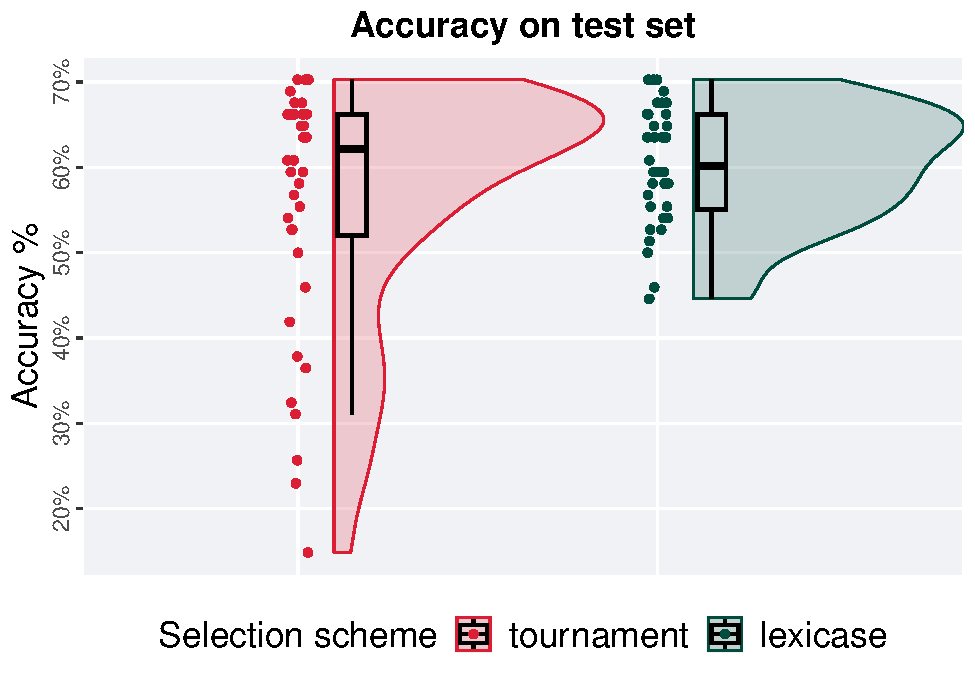
\includegraphics[width=1\linewidth]{lexidate-holdout-supplemental_files/figure-latex/task-359954-test-95-perf-1}

Summary statistics for the testing performance of the selection schemes at the 5\% selection set split:

\begin{Shaded}
\begin{Highlighting}[]
\FunctionTok{test\_results\_summary}\NormalTok{(}\FunctionTok{filter}\NormalTok{(task\_data, split }\SpecialCharTok{==} \StringTok{\textquotesingle{}95\%\textquotesingle{}}\NormalTok{))}
\end{Highlighting}
\end{Shaded}

\begin{verbatim}
## # A tibble: 2 x 8
##   selection  count na_cnt   min median  mean   max   IQR
##   <fct>      <int>  <int> <dbl>  <dbl> <dbl> <dbl> <dbl>
## 1 tournament    40      0 0.149  0.622 0.561 0.703 0.142
## 2 lexicase      40      0 0.446  0.601 0.601 0.703 0.111
\end{verbatim}

The permutation test revealed that the results are:

\begin{Shaded}
\begin{Highlighting}[]
\NormalTok{tournament\_results }\OtherTok{\textless{}{-}} \FunctionTok{filter}\NormalTok{(task\_data, split }\SpecialCharTok{==} \StringTok{\textquotesingle{}95\%\textquotesingle{}} \SpecialCharTok{\&}\NormalTok{ selection }\SpecialCharTok{==} \StringTok{\textquotesingle{}tournament\textquotesingle{}}\NormalTok{)}
\NormalTok{lexicase\_results }\OtherTok{\textless{}{-}} \FunctionTok{filter}\NormalTok{(task\_data, split }\SpecialCharTok{==} \StringTok{\textquotesingle{}95\%\textquotesingle{}} \SpecialCharTok{\&}\NormalTok{ selection }\SpecialCharTok{==} \StringTok{\textquotesingle{}lexicase\textquotesingle{}}\NormalTok{)}
\FunctionTok{permutation\_test}\NormalTok{(tournament\_results}\SpecialCharTok{$}\NormalTok{testing\_performance,}
\NormalTok{                    lexicase\_results}\SpecialCharTok{$}\NormalTok{testing\_performance,}
                    \AttributeTok{seed =} \DecValTok{19}\NormalTok{,}
                    \AttributeTok{alternative =} \StringTok{"t"}\NormalTok{)}
\end{Highlighting}
\end{Shaded}

\begin{verbatim}
## [1] "observed_diff: -1.54710562137524"
## [1] "lower: -1.95772948677679"
## [1] "upper: 1.95772969216945"
## [1] "fail to reject null hypothesis"
## [1] "p-value: 0.12617"
\end{verbatim}

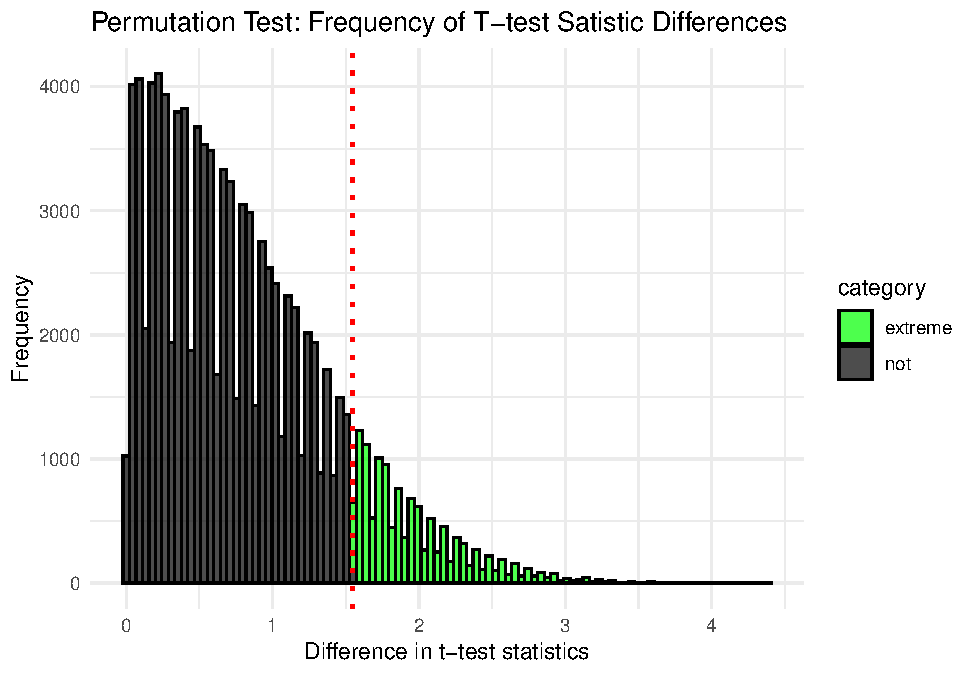
\includegraphics[width=1\linewidth]{lexidate-holdout-supplemental_files/figure-latex/task-359954-test-95-pv-1}

\hypertarget{selection-set-accuracy-9}{%
\subsection{Selection set accuracy}\label{selection-set-accuracy-9}}

\begin{Shaded}
\begin{Highlighting}[]
\FunctionTok{selection\_plot}\NormalTok{(}\FunctionTok{filter}\NormalTok{(task\_data, split }\SpecialCharTok{==} \StringTok{\textquotesingle{}95\%\textquotesingle{}}\NormalTok{))}
\end{Highlighting}
\end{Shaded}

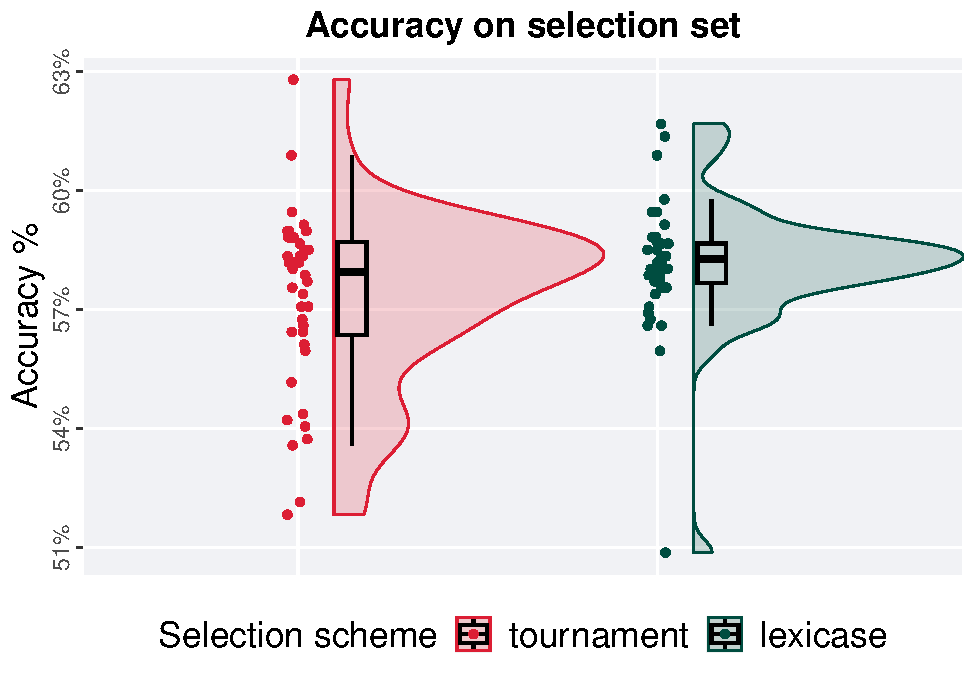
\includegraphics[width=1\linewidth]{lexidate-holdout-supplemental_files/figure-latex/task-359954-select-95-perf-1}

Summary statistics for the testing performance of the selection schemes at the 5\% selection set split:

\begin{Shaded}
\begin{Highlighting}[]
\FunctionTok{selection\_results\_summary}\NormalTok{(}\FunctionTok{filter}\NormalTok{(task\_data, split }\SpecialCharTok{==} \StringTok{\textquotesingle{}95\%\textquotesingle{}}\NormalTok{))}
\end{Highlighting}
\end{Shaded}

\begin{verbatim}
## # A tibble: 2 x 8
##   selection  count na_cnt   min median  mean   max     IQR
##   <fct>      <int>  <int> <dbl>  <dbl> <dbl> <dbl>   <dbl>
## 1 tournament    40      0 0.518  0.579 0.573 0.628 0.0234 
## 2 lexicase      40      0 0.509  0.583 0.582 0.617 0.00994
\end{verbatim}

The permutation test revealed that the results are:

\begin{Shaded}
\begin{Highlighting}[]
\NormalTok{tournament\_results }\OtherTok{\textless{}{-}} \FunctionTok{filter}\NormalTok{(task\_data, split }\SpecialCharTok{==} \StringTok{\textquotesingle{}95\%\textquotesingle{}} \SpecialCharTok{\&}\NormalTok{ selection }\SpecialCharTok{==} \StringTok{\textquotesingle{}tournament\textquotesingle{}}\NormalTok{)}
\NormalTok{lexicase\_results }\OtherTok{\textless{}{-}} \FunctionTok{filter}\NormalTok{(task\_data, split }\SpecialCharTok{==} \StringTok{\textquotesingle{}95\%\textquotesingle{}} \SpecialCharTok{\&}\NormalTok{ selection }\SpecialCharTok{==} \StringTok{\textquotesingle{}lexicase\textquotesingle{}}\NormalTok{)}
\FunctionTok{permutation\_test}\NormalTok{(tournament\_results}\SpecialCharTok{$}\NormalTok{training\_performance,}
\NormalTok{                    lexicase\_results}\SpecialCharTok{$}\NormalTok{training\_performance,}
                    \AttributeTok{seed =} \DecValTok{20}\NormalTok{,}
                    \AttributeTok{alternative =} \StringTok{"l"}\NormalTok{)}
\end{Highlighting}
\end{Shaded}

\begin{verbatim}
## [1] "observed_diff: -1.96456434004405"
## [1] "permutation_diffs[0.05 * n_permutations]: -1.64935315376094"
## [1] "reject null hypothesis"
## [1] "p-value: 0.02535"
\end{verbatim}

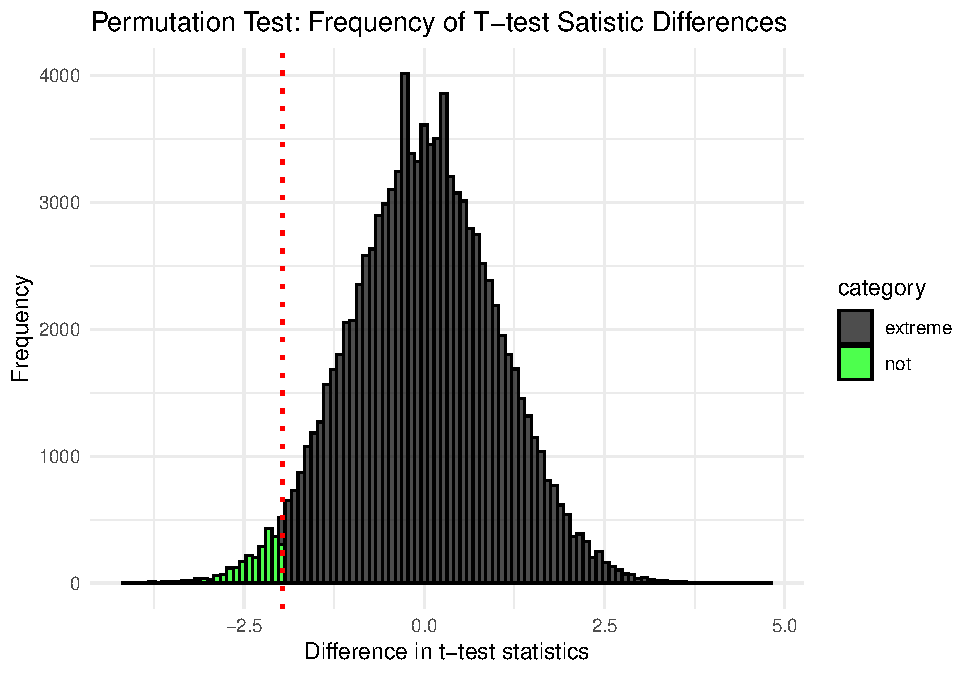
\includegraphics[width=1\linewidth]{lexidate-holdout-supplemental_files/figure-latex/task-359954-select-95-pv-1}

\hypertarget{task-359955}{%
\chapter{Task 359955}\label{task-359955}}

We present the results of our analysis of \texttt{task\ 359955} with the different selection set splits used in our study.

\begin{Shaded}
\begin{Highlighting}[]
\NormalTok{task\_data }\OtherTok{\textless{}{-}} \FunctionTok{filter}\NormalTok{(results, task\_id }\SpecialCharTok{==} \DecValTok{359955}\NormalTok{)}
\end{Highlighting}
\end{Shaded}

\hypertarget{section-10}\label{section-10}}

\hypertarget{testing-set-accuracy-10}{%
\subsection{Testing set accuracy}\label{testing-set-accuracy-10}}

\begin{Shaded}
\begin{Highlighting}[]
\FunctionTok{test\_plot}\NormalTok{(}\FunctionTok{filter}\NormalTok{(task\_data, split }\SpecialCharTok{==} \StringTok{\textquotesingle{}5\%\textquotesingle{}}\NormalTok{))}
\end{Highlighting}
\end{Shaded}

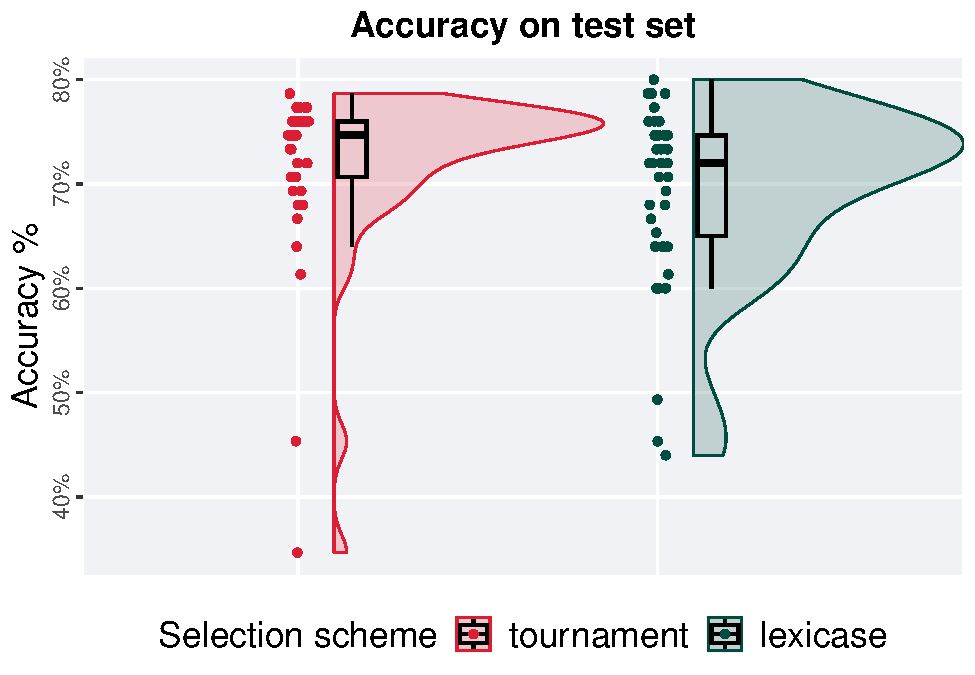
\includegraphics[width=1\linewidth]{lexidate-holdout-supplemental_files/figure-latex/task-359955-test-05-perf-1}

Summary statistics for the testing performance of the selection schemes at the 5\% selection set split:

\begin{Shaded}
\begin{Highlighting}[]
\FunctionTok{test\_results\_summary}\NormalTok{(}\FunctionTok{filter}\NormalTok{(task\_data, split }\SpecialCharTok{==} \StringTok{\textquotesingle{}5\%\textquotesingle{}}\NormalTok{))}
\end{Highlighting}
\end{Shaded}

\begin{verbatim}
## # A tibble: 2 x 8
##   selection  count na_cnt   min median  mean   max    IQR
##   <fct>      <int>  <int> <dbl>  <dbl> <dbl> <dbl>  <dbl>
## 1 tournament    40      0 0.347  0.747 0.719 0.787 0.0533
## 2 lexicase      40      0 0.44   0.72  0.694 0.8   0.0967
\end{verbatim}

The permutation test revealed that the results are:

\begin{Shaded}
\begin{Highlighting}[]
\NormalTok{tournament\_results }\OtherTok{\textless{}{-}} \FunctionTok{filter}\NormalTok{(task\_data, split }\SpecialCharTok{==} \StringTok{\textquotesingle{}5\%\textquotesingle{}} \SpecialCharTok{\&}\NormalTok{ selection }\SpecialCharTok{==} \StringTok{\textquotesingle{}tournament\textquotesingle{}}\NormalTok{)}
\NormalTok{lexicase\_results }\OtherTok{\textless{}{-}} \FunctionTok{filter}\NormalTok{(task\_data, split }\SpecialCharTok{==} \StringTok{\textquotesingle{}5\%\textquotesingle{}} \SpecialCharTok{\&}\NormalTok{ selection }\SpecialCharTok{==} \StringTok{\textquotesingle{}lexicase\textquotesingle{}}\NormalTok{)}
\FunctionTok{permutation\_test}\NormalTok{(tournament\_results}\SpecialCharTok{$}\NormalTok{testing\_performance,}
\NormalTok{                    lexicase\_results}\SpecialCharTok{$}\NormalTok{testing\_performance,}
                    \AttributeTok{seed =} \DecValTok{31}\NormalTok{,}
                    \AttributeTok{alternative =} \StringTok{"t"}\NormalTok{)}
\end{Highlighting}
\end{Shaded}

\begin{verbatim}
## [1] "observed_diff: 1.32499897361024"
## [1] "lower: -1.97890029487314"
## [1] "upper: 1.97890051754304"
## [1] "fail to reject null hypothesis"
## [1] "p-value: 0.19871"
\end{verbatim}

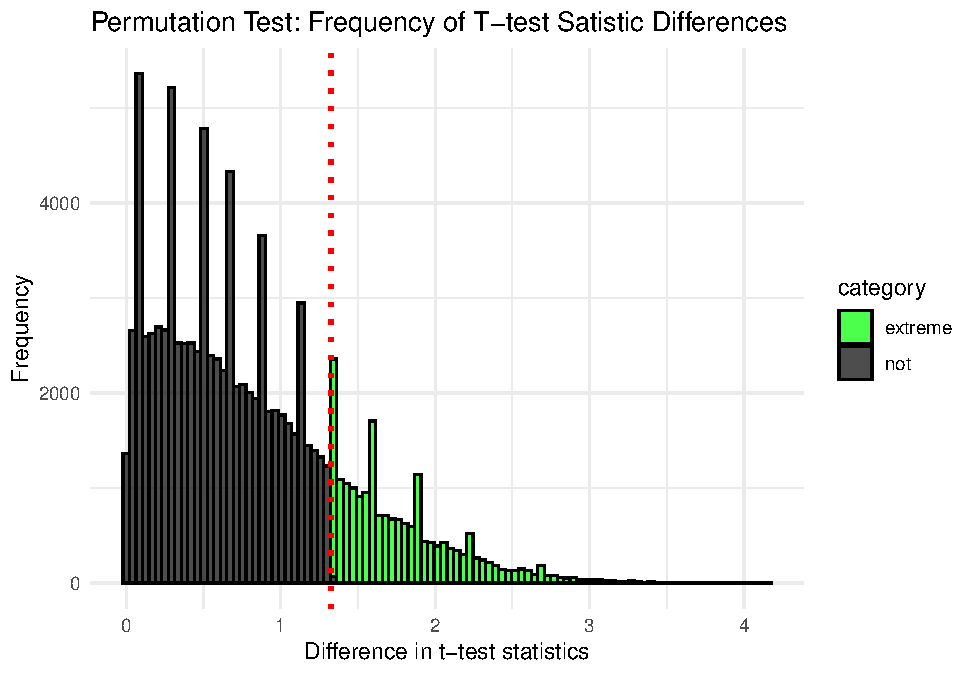
\includegraphics[width=1\linewidth]{lexidate-holdout-supplemental_files/figure-latex/task-359955-test-05-pv-1}

\hypertarget{selection-set-accuracy-10}{%
\subsection{Selection set accuracy}\label{selection-set-accuracy-10}}

\begin{Shaded}
\begin{Highlighting}[]
\FunctionTok{selection\_plot}\NormalTok{(}\FunctionTok{filter}\NormalTok{(task\_data, split }\SpecialCharTok{==} \StringTok{\textquotesingle{}5\%\textquotesingle{}}\NormalTok{))}
\end{Highlighting}
\end{Shaded}

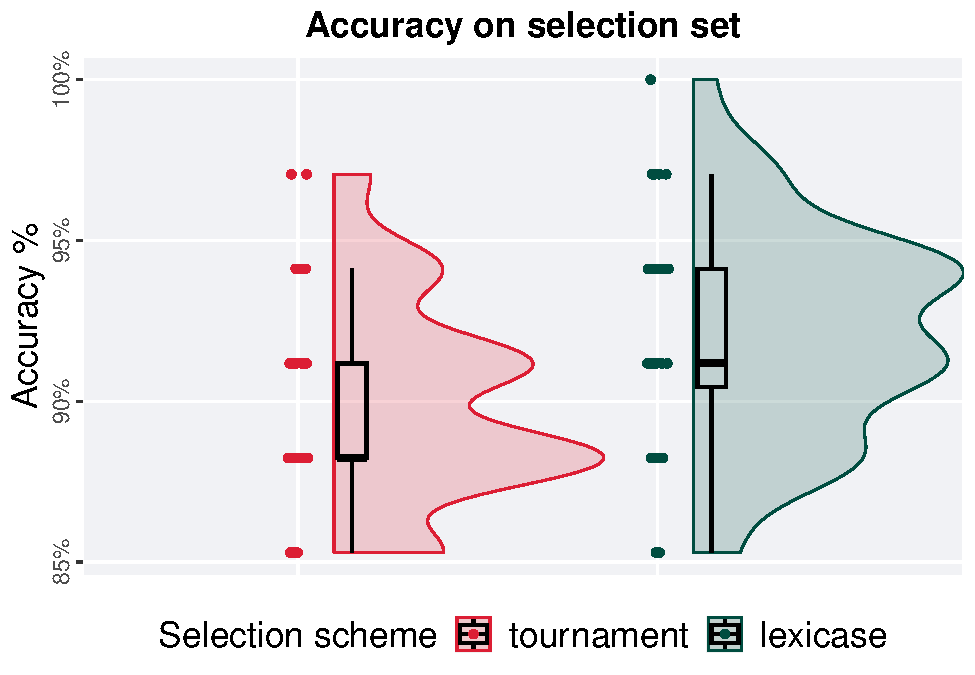
\includegraphics[width=1\linewidth]{lexidate-holdout-supplemental_files/figure-latex/task-359955-select-05-perf-1}

Summary statistics for the testing performance of the selection schemes at the 5\% selection set split:

\begin{Shaded}
\begin{Highlighting}[]
\FunctionTok{selection\_results\_summary}\NormalTok{(}\FunctionTok{filter}\NormalTok{(task\_data, split }\SpecialCharTok{==} \StringTok{\textquotesingle{}5\%\textquotesingle{}}\NormalTok{))}
\end{Highlighting}
\end{Shaded}

\begin{verbatim}
## # A tibble: 2 x 8
##   selection  count na_cnt   min median  mean   max    IQR
##   <fct>      <int>  <int> <dbl>  <dbl> <dbl> <dbl>  <dbl>
## 1 tournament    40      0 0.853  0.882 0.899 0.971 0.0294
## 2 lexicase      40      0 0.853  0.912 0.921 1     0.0368
\end{verbatim}

The permutation test revealed that the results are:

\begin{Shaded}
\begin{Highlighting}[]
\NormalTok{tournament\_results }\OtherTok{\textless{}{-}} \FunctionTok{filter}\NormalTok{(task\_data, split }\SpecialCharTok{==} \StringTok{\textquotesingle{}5\%\textquotesingle{}} \SpecialCharTok{\&}\NormalTok{ selection }\SpecialCharTok{==} \StringTok{\textquotesingle{}tournament\textquotesingle{}}\NormalTok{)}
\NormalTok{lexicase\_results }\OtherTok{\textless{}{-}} \FunctionTok{filter}\NormalTok{(task\_data, split }\SpecialCharTok{==} \StringTok{\textquotesingle{}5\%\textquotesingle{}} \SpecialCharTok{\&}\NormalTok{ selection }\SpecialCharTok{==} \StringTok{\textquotesingle{}lexicase\textquotesingle{}}\NormalTok{)}
\FunctionTok{permutation\_test}\NormalTok{(tournament\_results}\SpecialCharTok{$}\NormalTok{training\_performance,}
\NormalTok{                    lexicase\_results}\SpecialCharTok{$}\NormalTok{training\_performance,}
                    \AttributeTok{seed =} \DecValTok{32}\NormalTok{,}
                    \AttributeTok{alternative =} \StringTok{"l"}\NormalTok{)}
\end{Highlighting}
\end{Shaded}

\begin{verbatim}
## [1] "observed_diff: -2.91990855742165"
## [1] "permutation_diffs[0.05 * n_permutations]: -1.65338713426272"
## [1] "reject null hypothesis"
## [1] "p-value: 0.00214"
\end{verbatim}

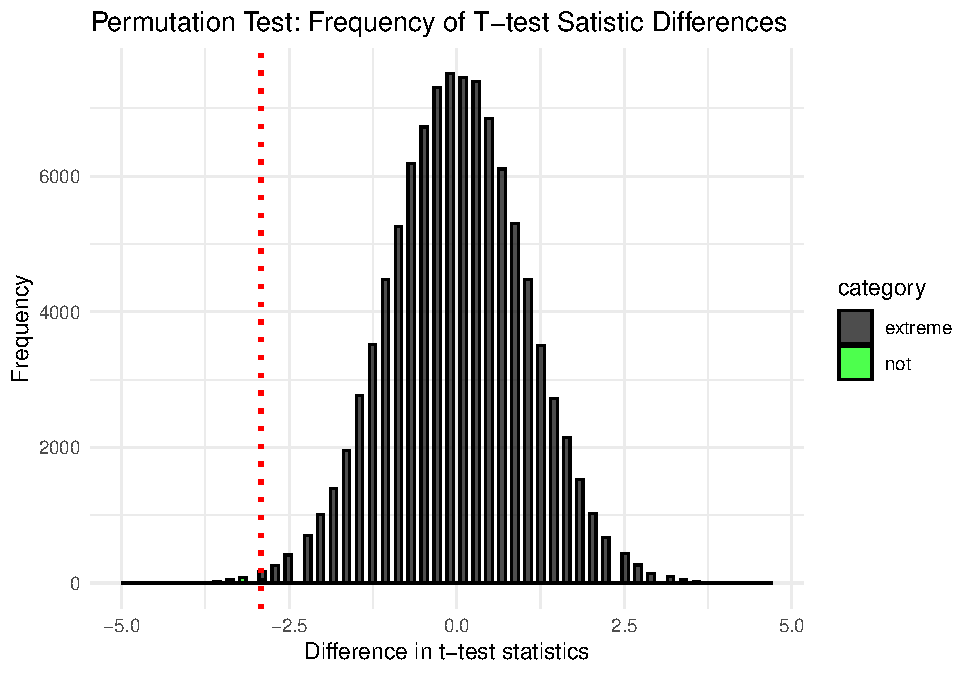
\includegraphics[width=1\linewidth]{lexidate-holdout-supplemental_files/figure-latex/task-359955-select-05-pv-1}

\hypertarget{section-11}\label{section-11}}

\hypertarget{testing-set-accuracy-11}{%
\subsection{Testing set accuracy}\label{testing-set-accuracy-11}}

\begin{Shaded}
\begin{Highlighting}[]
\FunctionTok{test\_plot}\NormalTok{(}\FunctionTok{filter}\NormalTok{(task\_data, split }\SpecialCharTok{==} \StringTok{\textquotesingle{}10\%\textquotesingle{}}\NormalTok{))}
\end{Highlighting}
\end{Shaded}

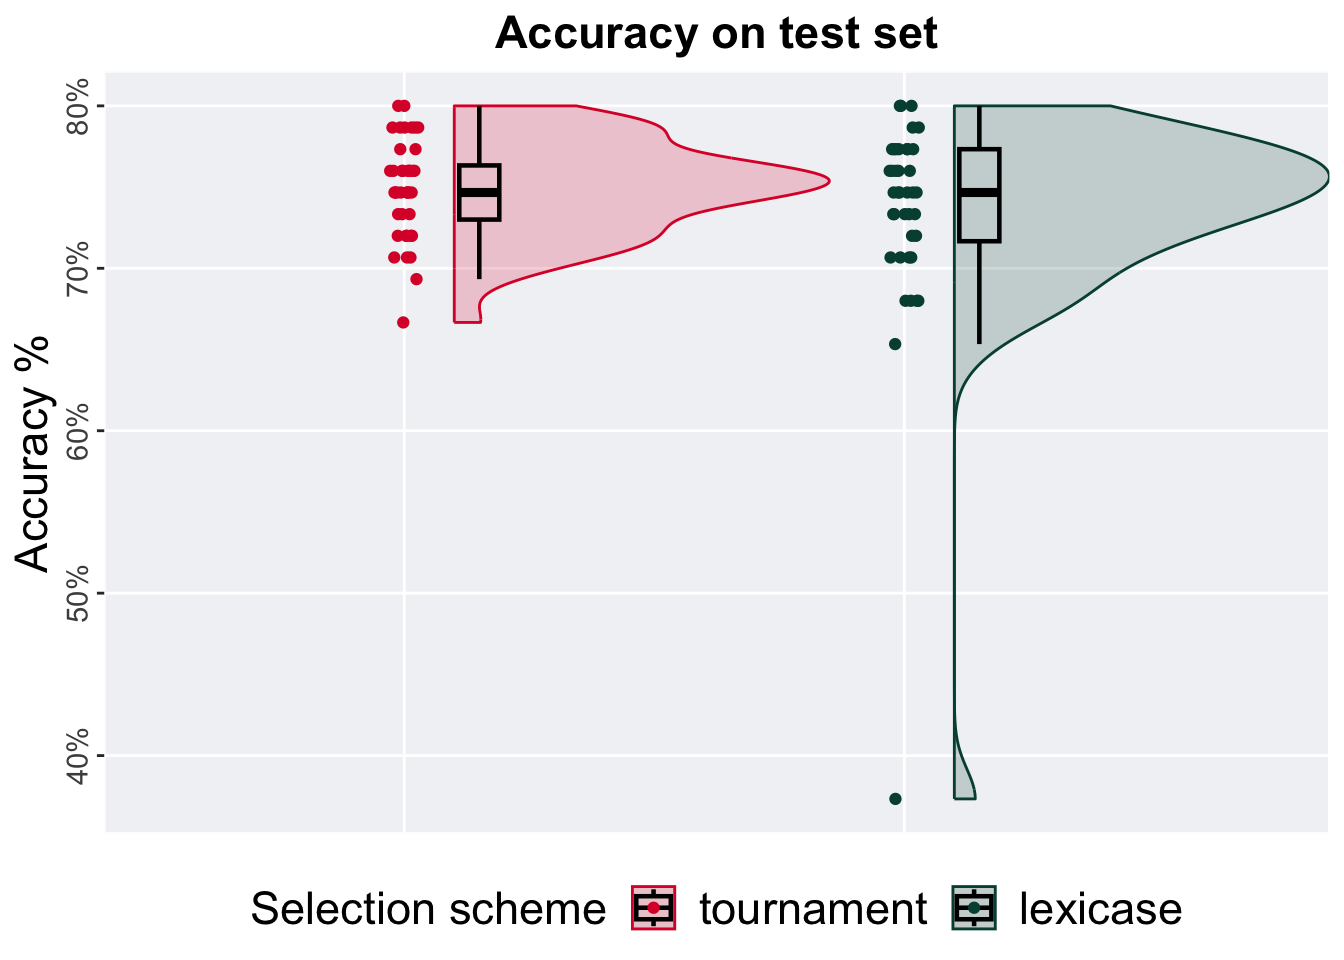
\includegraphics[width=1\linewidth]{lexidate-holdout-supplemental_files/figure-latex/task-359955-test-10-perf-1}

Summary statistics for the testing performance of the selection schemes at the 5\% selection set split:

\begin{Shaded}
\begin{Highlighting}[]
\FunctionTok{test\_results\_summary}\NormalTok{(}\FunctionTok{filter}\NormalTok{(task\_data, split }\SpecialCharTok{==} \StringTok{\textquotesingle{}10\%\textquotesingle{}}\NormalTok{))}
\end{Highlighting}
\end{Shaded}

\begin{verbatim}
## # A tibble: 2 x 8
##   selection  count na_cnt   min median  mean   max    IQR
##   <fct>      <int>  <int> <dbl>  <dbl> <dbl> <dbl>  <dbl>
## 1 tournament    40      0 0.667  0.747 0.749   0.8 0.0333
## 2 lexicase      40      0 0.373  0.747 0.734   0.8 0.0567
\end{verbatim}

The permutation test revealed that the results are:

\begin{Shaded}
\begin{Highlighting}[]
\NormalTok{tournament\_results }\OtherTok{\textless{}{-}} \FunctionTok{filter}\NormalTok{(task\_data, split }\SpecialCharTok{==} \StringTok{\textquotesingle{}10\%\textquotesingle{}} \SpecialCharTok{\&}\NormalTok{ selection }\SpecialCharTok{==} \StringTok{\textquotesingle{}tournament\textquotesingle{}}\NormalTok{)}
\NormalTok{lexicase\_results }\OtherTok{\textless{}{-}} \FunctionTok{filter}\NormalTok{(task\_data, split }\SpecialCharTok{==} \StringTok{\textquotesingle{}10\%\textquotesingle{}} \SpecialCharTok{\&}\NormalTok{ selection }\SpecialCharTok{==} \StringTok{\textquotesingle{}lexicase\textquotesingle{}}\NormalTok{)}
\FunctionTok{permutation\_test}\NormalTok{(tournament\_results}\SpecialCharTok{$}\NormalTok{testing\_performance,}
\NormalTok{                    lexicase\_results}\SpecialCharTok{$}\NormalTok{testing\_performance,}
                    \AttributeTok{seed =} \DecValTok{33}\NormalTok{,}
                    \AttributeTok{alternative =} \StringTok{"t"}\NormalTok{)}
\end{Highlighting}
\end{Shaded}

\begin{verbatim}
## [1] "observed_diff: 1.28638411846571"
## [1] "lower: -1.86676173626107"
## [1] "upper: 1.80778536386294"
## [1] "fail to reject null hypothesis"
## [1] "p-value: 0.20426"
\end{verbatim}

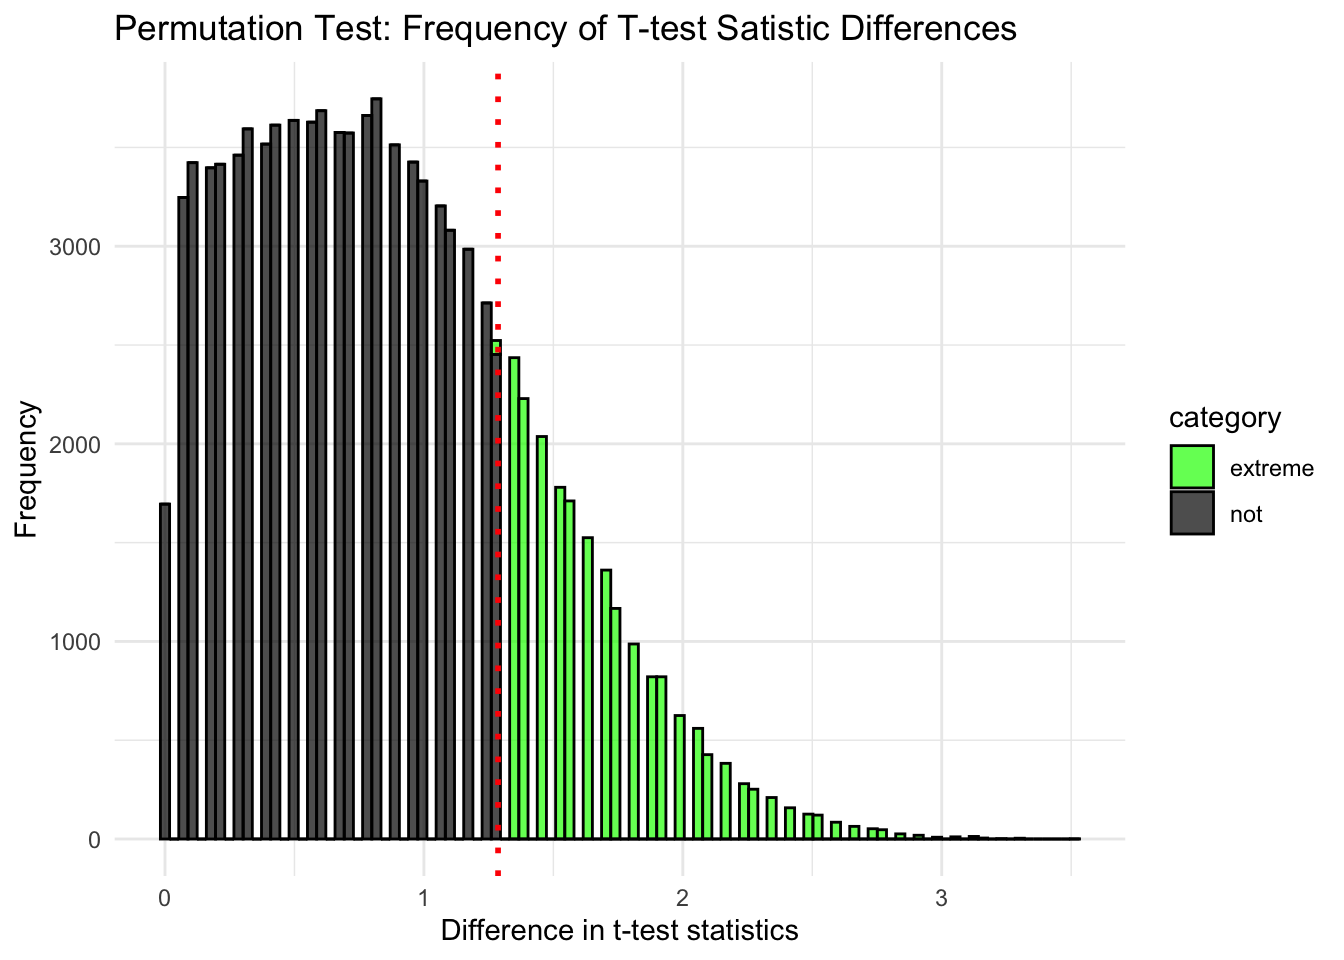
\includegraphics[width=1\linewidth]{lexidate-holdout-supplemental_files/figure-latex/task-359955-test-10-pv-1}

\hypertarget{selection-set-accuracy-11}{%
\subsection{Selection set accuracy}\label{selection-set-accuracy-11}}

\begin{Shaded}
\begin{Highlighting}[]
\FunctionTok{selection\_plot}\NormalTok{(}\FunctionTok{filter}\NormalTok{(task\_data, split }\SpecialCharTok{==} \StringTok{\textquotesingle{}10\%\textquotesingle{}}\NormalTok{))}
\end{Highlighting}
\end{Shaded}

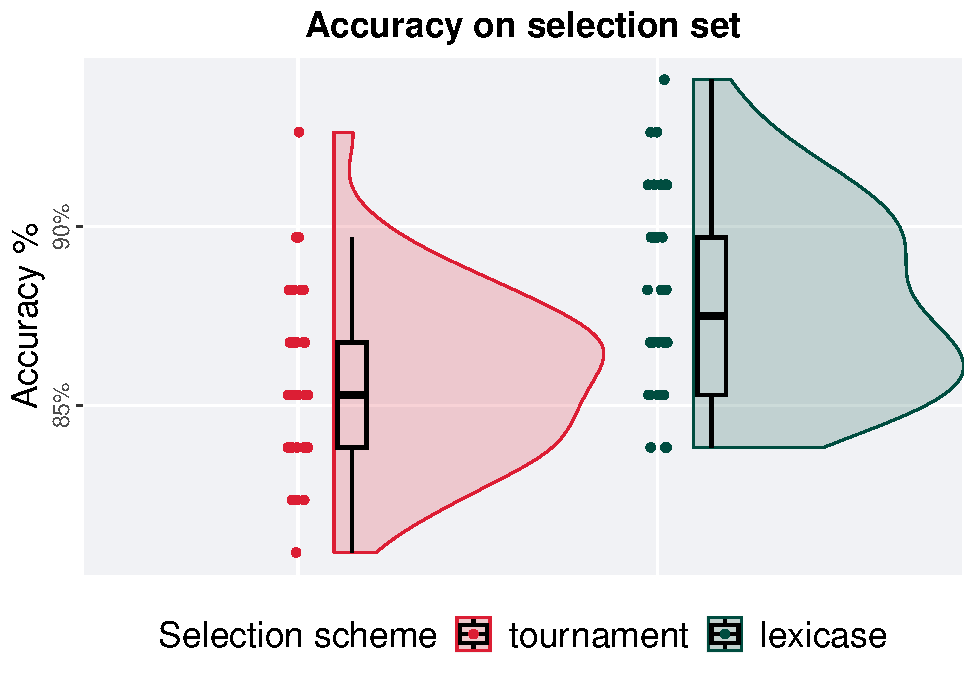
\includegraphics[width=1\linewidth]{lexidate-holdout-supplemental_files/figure-latex/task-359955-select-10-perf-1}

Summary statistics for the testing performance of the selection schemes at the 5\% selection set split:

\begin{Shaded}
\begin{Highlighting}[]
\FunctionTok{selection\_results\_summary}\NormalTok{(}\FunctionTok{filter}\NormalTok{(task\_data, split }\SpecialCharTok{==} \StringTok{\textquotesingle{}10\%\textquotesingle{}}\NormalTok{))}
\end{Highlighting}
\end{Shaded}

\begin{verbatim}
## # A tibble: 2 x 8
##   selection  count na_cnt   min median  mean   max    IQR
##   <fct>      <int>  <int> <dbl>  <dbl> <dbl> <dbl>  <dbl>
## 1 tournament    40      0 0.809  0.853 0.858 0.926 0.0294
## 2 lexicase      40      0 0.838  0.875 0.879 0.941 0.0441
\end{verbatim}

The permutation test revealed that the results are:

\begin{Shaded}
\begin{Highlighting}[]
\NormalTok{tournament\_results }\OtherTok{\textless{}{-}} \FunctionTok{filter}\NormalTok{(task\_data, split }\SpecialCharTok{==} \StringTok{\textquotesingle{}10\%\textquotesingle{}} \SpecialCharTok{\&}\NormalTok{ selection }\SpecialCharTok{==} \StringTok{\textquotesingle{}tournament\textquotesingle{}}\NormalTok{)}
\NormalTok{lexicase\_results }\OtherTok{\textless{}{-}} \FunctionTok{filter}\NormalTok{(task\_data, split }\SpecialCharTok{==} \StringTok{\textquotesingle{}10\%\textquotesingle{}} \SpecialCharTok{\&}\NormalTok{ selection }\SpecialCharTok{==} \StringTok{\textquotesingle{}lexicase\textquotesingle{}}\NormalTok{)}
\FunctionTok{permutation\_test}\NormalTok{(tournament\_results}\SpecialCharTok{$}\NormalTok{training\_performance,}
\NormalTok{                    lexicase\_results}\SpecialCharTok{$}\NormalTok{training\_performance,}
                    \AttributeTok{seed =} \DecValTok{34}\NormalTok{,}
                    \AttributeTok{alternative =} \StringTok{"l"}\NormalTok{)}
\end{Highlighting}
\end{Shaded}

\begin{verbatim}
## [1] "observed_diff: -3.7319412515713"
## [1] "permutation_diffs[0.05 * n_permutations]: -1.68964535023223"
## [1] "reject null hypothesis"
## [1] "p-value: 0.00019"
\end{verbatim}

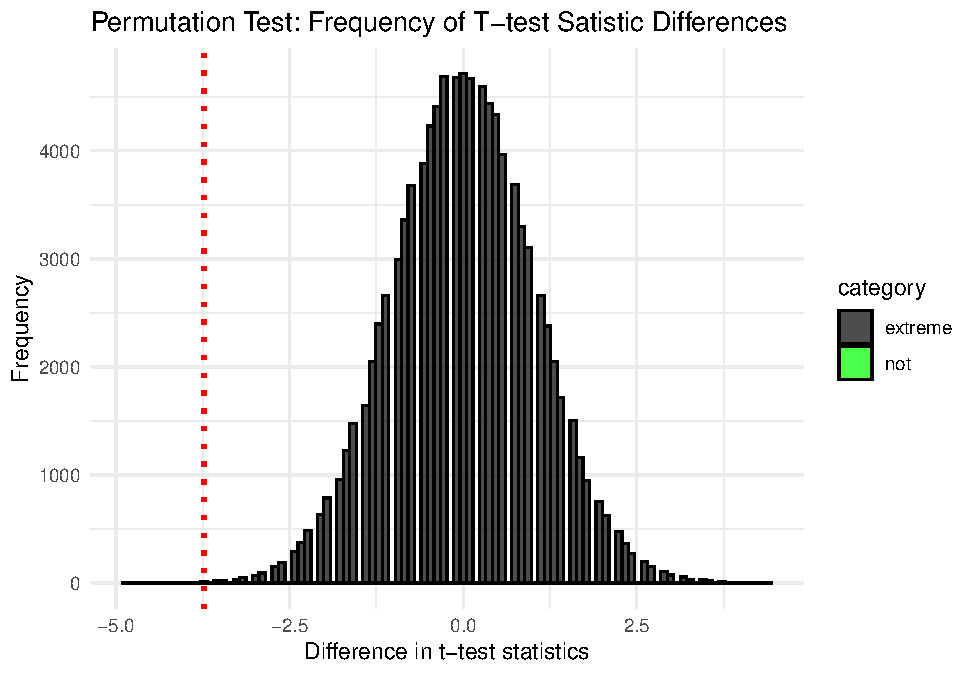
\includegraphics[width=1\linewidth]{lexidate-holdout-supplemental_files/figure-latex/task-359955-select-10-pv-1}

\hypertarget{section-12}\label{section-12}}

\hypertarget{testing-set-accuracy-12}{%
\subsection{Testing set accuracy}\label{testing-set-accuracy-12}}

\begin{Shaded}
\begin{Highlighting}[]
\FunctionTok{test\_plot}\NormalTok{(}\FunctionTok{filter}\NormalTok{(task\_data, split }\SpecialCharTok{==} \StringTok{\textquotesingle{}50\%\textquotesingle{}}\NormalTok{))}
\end{Highlighting}
\end{Shaded}

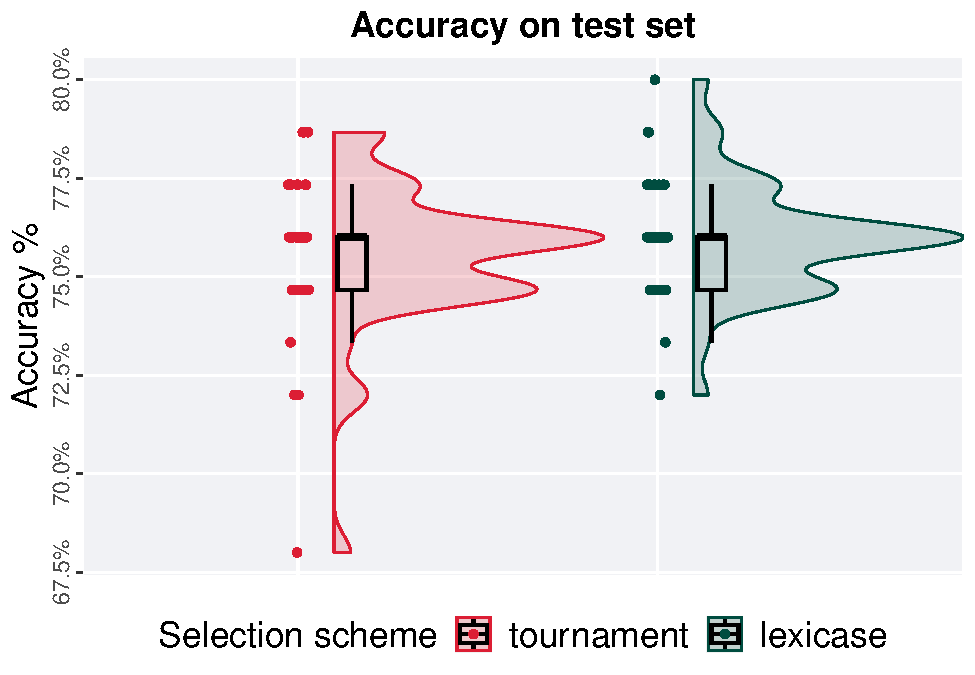
\includegraphics[width=1\linewidth]{lexidate-holdout-supplemental_files/figure-latex/task-359955-test-50-perf-1}

Summary statistics for the testing performance of the selection schemes at the 5\% selection set split:

\begin{Shaded}
\begin{Highlighting}[]
\FunctionTok{test\_results\_summary}\NormalTok{(}\FunctionTok{filter}\NormalTok{(task\_data, split }\SpecialCharTok{==} \StringTok{\textquotesingle{}50\%\textquotesingle{}}\NormalTok{))}
\end{Highlighting}
\end{Shaded}

\begin{verbatim}
## # A tibble: 2 x 8
##   selection  count na_cnt   min median  mean   max    IQR
##   <fct>      <int>  <int> <dbl>  <dbl> <dbl> <dbl>  <dbl>
## 1 tournament    40      0  0.68   0.76 0.755 0.787 0.0133
## 2 lexicase      40      0  0.72   0.76 0.759 0.8   0.0133
\end{verbatim}

The permutation test revealed that the results are:

\begin{Shaded}
\begin{Highlighting}[]
\NormalTok{tournament\_results }\OtherTok{\textless{}{-}} \FunctionTok{filter}\NormalTok{(task\_data, split }\SpecialCharTok{==} \StringTok{\textquotesingle{}50\%\textquotesingle{}} \SpecialCharTok{\&}\NormalTok{ selection }\SpecialCharTok{==} \StringTok{\textquotesingle{}tournament\textquotesingle{}}\NormalTok{)}
\NormalTok{lexicase\_results }\OtherTok{\textless{}{-}} \FunctionTok{filter}\NormalTok{(task\_data, split }\SpecialCharTok{==} \StringTok{\textquotesingle{}50\%\textquotesingle{}} \SpecialCharTok{\&}\NormalTok{ selection }\SpecialCharTok{==} \StringTok{\textquotesingle{}lexicase\textquotesingle{}}\NormalTok{)}
\FunctionTok{permutation\_test}\NormalTok{(tournament\_results}\SpecialCharTok{$}\NormalTok{testing\_performance,}
\NormalTok{                    lexicase\_results}\SpecialCharTok{$}\NormalTok{testing\_performance,}
                    \AttributeTok{seed =} \DecValTok{35}\NormalTok{,}
                    \AttributeTok{alternative =} \StringTok{"t"}\NormalTok{)}
\end{Highlighting}
\end{Shaded}

\begin{verbatim}
## [1] "observed_diff: -1.13782106538951"
## [1] "lower: -2.04962738612793"
## [1] "upper: 2.04962752699874"
## [1] "fail to reject null hypothesis"
## [1] "p-value: 0.27624"
\end{verbatim}

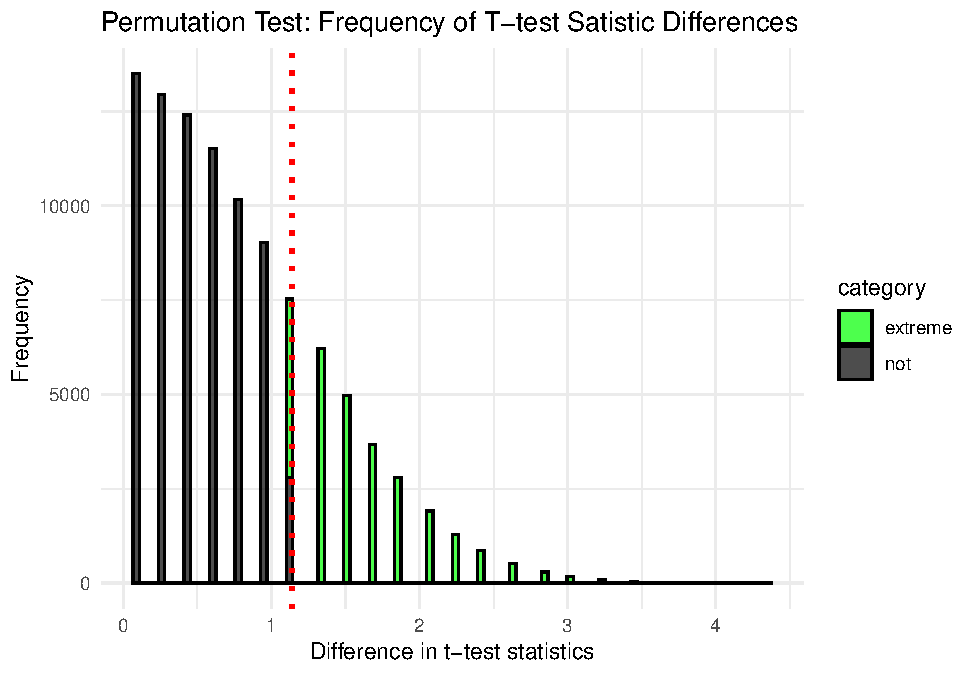
\includegraphics[width=1\linewidth]{lexidate-holdout-supplemental_files/figure-latex/task-359955-test-50-pv-1}

\hypertarget{selection-set-accuracy-12}{%
\subsection{Selection set accuracy}\label{selection-set-accuracy-12}}

\begin{Shaded}
\begin{Highlighting}[]
\FunctionTok{selection\_plot}\NormalTok{(}\FunctionTok{filter}\NormalTok{(task\_data, split }\SpecialCharTok{==} \StringTok{\textquotesingle{}50\%\textquotesingle{}}\NormalTok{))}
\end{Highlighting}
\end{Shaded}

\includegraphics[width=1\linewidth]{lexidate-holdout-supplemental_files/figure-latex/task-359955-select-50-perf-1}

Summary statistics for the testing performance of the selection schemes at the 5\% selection set split:

\begin{Shaded}
\begin{Highlighting}[]
\FunctionTok{selection\_results\_summary}\NormalTok{(}\FunctionTok{filter}\NormalTok{(task\_data, split }\SpecialCharTok{==} \StringTok{\textquotesingle{}50\%\textquotesingle{}}\NormalTok{))}
\end{Highlighting}
\end{Shaded}

\begin{verbatim}
## # A tibble: 2 x 8
##   selection  count na_cnt   min median  mean   max    IQR
##   <fct>      <int>  <int> <dbl>  <dbl> <dbl> <dbl>  <dbl>
## 1 tournament    40      0 0.801  0.818 0.817 0.834 0.0104
## 2 lexicase      40      0 0.795  0.813 0.816 0.837 0.0148
\end{verbatim}

The permutation test revealed that the results are:

\begin{Shaded}
\begin{Highlighting}[]
\NormalTok{tournament\_results }\OtherTok{\textless{}{-}} \FunctionTok{filter}\NormalTok{(task\_data, split }\SpecialCharTok{==} \StringTok{\textquotesingle{}50\%\textquotesingle{}} \SpecialCharTok{\&}\NormalTok{ selection }\SpecialCharTok{==} \StringTok{\textquotesingle{}tournament\textquotesingle{}}\NormalTok{)}
\NormalTok{lexicase\_results }\OtherTok{\textless{}{-}} \FunctionTok{filter}\NormalTok{(task\_data, split }\SpecialCharTok{==} \StringTok{\textquotesingle{}50\%\textquotesingle{}} \SpecialCharTok{\&}\NormalTok{ selection }\SpecialCharTok{==} \StringTok{\textquotesingle{}lexicase\textquotesingle{}}\NormalTok{)}
\FunctionTok{permutation\_test}\NormalTok{(tournament\_results}\SpecialCharTok{$}\NormalTok{training\_performance,}
\NormalTok{                    lexicase\_results}\SpecialCharTok{$}\NormalTok{training\_performance,}
                    \AttributeTok{seed =} \DecValTok{36}\NormalTok{,}
                    \AttributeTok{alternative =} \StringTok{"t"}\NormalTok{)}
\end{Highlighting}
\end{Shaded}

\begin{verbatim}
## [1] "observed_diff: 0.475399664870139"
## [1] "lower: -1.9835828407878"
## [1] "upper: 1.98358257581197"
## [1] "fail to reject null hypothesis"
## [1] "p-value: 0.64083"
\end{verbatim}

\includegraphics[width=1\linewidth]{lexidate-holdout-supplemental_files/figure-latex/task-359955-select-50-pv-1}

\hypertarget{section-13}\label{section-13}}

\hypertarget{testing-set-accuracy-13}{%
\subsection{Testing set accuracy}\label{testing-set-accuracy-13}}

\begin{Shaded}
\begin{Highlighting}[]
\FunctionTok{test\_plot}\NormalTok{(}\FunctionTok{filter}\NormalTok{(task\_data, split }\SpecialCharTok{==} \StringTok{\textquotesingle{}90\%\textquotesingle{}}\NormalTok{))}
\end{Highlighting}
\end{Shaded}

\includegraphics[width=1\linewidth]{lexidate-holdout-supplemental_files/figure-latex/task-359955-test-90-perf-1}

Summary statistics for the testing performance of the selection schemes at the 5\% selection set split:

\begin{Shaded}
\begin{Highlighting}[]
\FunctionTok{test\_results\_summary}\NormalTok{(}\FunctionTok{filter}\NormalTok{(task\_data, split }\SpecialCharTok{==} \StringTok{\textquotesingle{}90\%\textquotesingle{}}\NormalTok{))}
\end{Highlighting}
\end{Shaded}

\begin{verbatim}
## # A tibble: 2 x 8
##   selection  count na_cnt   min median  mean   max    IQR
##   <fct>      <int>  <int> <dbl>  <dbl> <dbl> <dbl>  <dbl>
## 1 tournament    40      0 0.28    0.76 0.731 0.787 0.0267
## 2 lexicase      40      0 0.693   0.76 0.759 0.813 0.0267
\end{verbatim}

The permutation test revealed that the results are:

\begin{Shaded}
\begin{Highlighting}[]
\NormalTok{tournament\_results }\OtherTok{\textless{}{-}} \FunctionTok{filter}\NormalTok{(task\_data, split }\SpecialCharTok{==} \StringTok{\textquotesingle{}90\%\textquotesingle{}} \SpecialCharTok{\&}\NormalTok{ selection }\SpecialCharTok{==} \StringTok{\textquotesingle{}tournament\textquotesingle{}}\NormalTok{)}
\NormalTok{lexicase\_results }\OtherTok{\textless{}{-}} \FunctionTok{filter}\NormalTok{(task\_data, split }\SpecialCharTok{==} \StringTok{\textquotesingle{}90\%\textquotesingle{}} \SpecialCharTok{\&}\NormalTok{ selection }\SpecialCharTok{==} \StringTok{\textquotesingle{}lexicase\textquotesingle{}}\NormalTok{)}
\FunctionTok{permutation\_test}\NormalTok{(tournament\_results}\SpecialCharTok{$}\NormalTok{testing\_performance,}
\NormalTok{                    lexicase\_results}\SpecialCharTok{$}\NormalTok{testing\_performance,}
                    \AttributeTok{seed =} \DecValTok{37}\NormalTok{,}
                    \AttributeTok{alternative =} \StringTok{"l"}\NormalTok{)}
\end{Highlighting}
\end{Shaded}

\begin{verbatim}
## [1] "observed_diff: -2.01490383284339"
## [1] "permutation_diffs[0.05 * n_permutations]: -1.56760535956015"
## [1] "reject null hypothesis"
## [1] "p-value: 0.00738"
\end{verbatim}

\includegraphics[width=1\linewidth]{lexidate-holdout-supplemental_files/figure-latex/task-359955-test-90-pv-1}

\hypertarget{selection-set-accuracy-13}{%
\subsection{Selection set accuracy}\label{selection-set-accuracy-13}}

\begin{Shaded}
\begin{Highlighting}[]
\FunctionTok{selection\_plot}\NormalTok{(}\FunctionTok{filter}\NormalTok{(task\_data, split }\SpecialCharTok{==} \StringTok{\textquotesingle{}90\%\textquotesingle{}}\NormalTok{))}
\end{Highlighting}
\end{Shaded}

\includegraphics[width=1\linewidth]{lexidate-holdout-supplemental_files/figure-latex/task-359955-select-90-perf-1}

Summary statistics for the testing performance of the selection schemes at the 5\% selection set split:

\begin{Shaded}
\begin{Highlighting}[]
\FunctionTok{selection\_results\_summary}\NormalTok{(}\FunctionTok{filter}\NormalTok{(task\_data, split }\SpecialCharTok{==} \StringTok{\textquotesingle{}90\%\textquotesingle{}}\NormalTok{))}
\end{Highlighting}
\end{Shaded}

\begin{verbatim}
## # A tibble: 2 x 8
##   selection  count na_cnt   min median  mean   max     IQR
##   <fct>      <int>  <int> <dbl>  <dbl> <dbl> <dbl>   <dbl>
## 1 tournament    40      0 0.792  0.802 0.802 0.814 0.00866
## 2 lexicase      40      0 0.794  0.804 0.803 0.815 0.00825
\end{verbatim}

The permutation test revealed that the results are:

\begin{Shaded}
\begin{Highlighting}[]
\NormalTok{tournament\_results }\OtherTok{\textless{}{-}} \FunctionTok{filter}\NormalTok{(task\_data, split }\SpecialCharTok{==} \StringTok{\textquotesingle{}90\%\textquotesingle{}} \SpecialCharTok{\&}\NormalTok{ selection }\SpecialCharTok{==} \StringTok{\textquotesingle{}tournament\textquotesingle{}}\NormalTok{)}
\NormalTok{lexicase\_results }\OtherTok{\textless{}{-}} \FunctionTok{filter}\NormalTok{(task\_data, split }\SpecialCharTok{==} \StringTok{\textquotesingle{}90\%\textquotesingle{}} \SpecialCharTok{\&}\NormalTok{ selection }\SpecialCharTok{==} \StringTok{\textquotesingle{}lexicase\textquotesingle{}}\NormalTok{)}
\FunctionTok{permutation\_test}\NormalTok{(tournament\_results}\SpecialCharTok{$}\NormalTok{training\_performance,}
\NormalTok{                    lexicase\_results}\SpecialCharTok{$}\NormalTok{training\_performance,}
                    \AttributeTok{seed =} \DecValTok{38}\NormalTok{,}
                    \AttributeTok{alternative =} \StringTok{"t"}\NormalTok{)}
\end{Highlighting}
\end{Shaded}

\begin{verbatim}
## [1] "observed_diff: -1.30766861645993"
## [1] "lower: -1.97012862430494"
## [1] "upper: 1.97013135879071"
## [1] "fail to reject null hypothesis"
## [1] "p-value: 0.19023"
\end{verbatim}

\includegraphics[width=1\linewidth]{lexidate-holdout-supplemental_files/figure-latex/task-359955-select-90-pv-1}

\hypertarget{section-14}\label{section-14}}

\hypertarget{testing-set-accuracy-14}{%
\subsection{Testing set accuracy}\label{testing-set-accuracy-14}}

\begin{Shaded}
\begin{Highlighting}[]
\FunctionTok{test\_plot}\NormalTok{(}\FunctionTok{filter}\NormalTok{(task\_data, split }\SpecialCharTok{==} \StringTok{\textquotesingle{}95\%\textquotesingle{}}\NormalTok{))}
\end{Highlighting}
\end{Shaded}

\includegraphics[width=1\linewidth]{lexidate-holdout-supplemental_files/figure-latex/task-359955-test-95-perf-1}

Summary statistics for the testing performance of the selection schemes at the 5\% selection set split:

\begin{Shaded}
\begin{Highlighting}[]
\FunctionTok{test\_results\_summary}\NormalTok{(}\FunctionTok{filter}\NormalTok{(task\_data, split }\SpecialCharTok{==} \StringTok{\textquotesingle{}95\%\textquotesingle{}}\NormalTok{))}
\end{Highlighting}
\end{Shaded}

\begin{verbatim}
## # A tibble: 2 x 8
##   selection  count na_cnt   min median  mean   max    IQR
##   <fct>      <int>  <int> <dbl>  <dbl> <dbl> <dbl>  <dbl>
## 1 tournament    40      0 0.253   0.76 0.733 0.773 0.0267
## 2 lexicase      40      0 0.573   0.76 0.735 0.8   0.0300
\end{verbatim}

The permutation test revealed that the results are:

\begin{Shaded}
\begin{Highlighting}[]
\NormalTok{tournament\_results }\OtherTok{\textless{}{-}} \FunctionTok{filter}\NormalTok{(task\_data, split }\SpecialCharTok{==} \StringTok{\textquotesingle{}95\%\textquotesingle{}} \SpecialCharTok{\&}\NormalTok{ selection }\SpecialCharTok{==} \StringTok{\textquotesingle{}tournament\textquotesingle{}}\NormalTok{)}
\NormalTok{lexicase\_results }\OtherTok{\textless{}{-}} \FunctionTok{filter}\NormalTok{(task\_data, split }\SpecialCharTok{==} \StringTok{\textquotesingle{}95\%\textquotesingle{}} \SpecialCharTok{\&}\NormalTok{ selection }\SpecialCharTok{==} \StringTok{\textquotesingle{}lexicase\textquotesingle{}}\NormalTok{)}
\FunctionTok{permutation\_test}\NormalTok{(tournament\_results}\SpecialCharTok{$}\NormalTok{testing\_performance,}
\NormalTok{                    lexicase\_results}\SpecialCharTok{$}\NormalTok{testing\_performance,}
                    \AttributeTok{seed =} \DecValTok{39}\NormalTok{,}
                    \AttributeTok{alternative =} \StringTok{"t"}\NormalTok{)}
\end{Highlighting}
\end{Shaded}

\begin{verbatim}
## [1] "observed_diff: -0.170085425997122"
## [1] "lower: -1.82321742524129"
## [1] "upper: 1.8232173573514"
## [1] "fail to reject null hypothesis"
## [1] "p-value: 0.89693"
\end{verbatim}

\includegraphics[width=1\linewidth]{lexidate-holdout-supplemental_files/figure-latex/task-359955-test-95-pv-1}

\hypertarget{selection-set-accuracy-14}{%
\subsection{Selection set accuracy}\label{selection-set-accuracy-14}}

\begin{Shaded}
\begin{Highlighting}[]
\FunctionTok{selection\_plot}\NormalTok{(}\FunctionTok{filter}\NormalTok{(task\_data, split }\SpecialCharTok{==} \StringTok{\textquotesingle{}95\%\textquotesingle{}}\NormalTok{))}
\end{Highlighting}
\end{Shaded}

\includegraphics[width=1\linewidth]{lexidate-holdout-supplemental_files/figure-latex/task-359955-select-95-perf-1}

Summary statistics for the testing performance of the selection schemes at the 5\% selection set split:

\begin{Shaded}
\begin{Highlighting}[]
\FunctionTok{selection\_results\_summary}\NormalTok{(}\FunctionTok{filter}\NormalTok{(task\_data, split }\SpecialCharTok{==} \StringTok{\textquotesingle{}95\%\textquotesingle{}}\NormalTok{))}
\end{Highlighting}
\end{Shaded}

\begin{verbatim}
## # A tibble: 2 x 8
##   selection  count na_cnt   min median  mean   max     IQR
##   <fct>      <int>  <int> <dbl>  <dbl> <dbl> <dbl>   <dbl>
## 1 tournament    40      0 0.789  0.798 0.799 0.811 0.00625
## 2 lexicase      40      0 0.788  0.801 0.801 0.808 0.00664
\end{verbatim}

The permutation test revealed that the results are:

\begin{Shaded}
\begin{Highlighting}[]
\NormalTok{tournament\_results }\OtherTok{\textless{}{-}} \FunctionTok{filter}\NormalTok{(task\_data, split }\SpecialCharTok{==} \StringTok{\textquotesingle{}95\%\textquotesingle{}} \SpecialCharTok{\&}\NormalTok{ selection }\SpecialCharTok{==} \StringTok{\textquotesingle{}tournament\textquotesingle{}}\NormalTok{)}
\NormalTok{lexicase\_results }\OtherTok{\textless{}{-}} \FunctionTok{filter}\NormalTok{(task\_data, split }\SpecialCharTok{==} \StringTok{\textquotesingle{}95\%\textquotesingle{}} \SpecialCharTok{\&}\NormalTok{ selection }\SpecialCharTok{==} \StringTok{\textquotesingle{}lexicase\textquotesingle{}}\NormalTok{)}
\FunctionTok{permutation\_test}\NormalTok{(tournament\_results}\SpecialCharTok{$}\NormalTok{training\_performance,}
\NormalTok{                    lexicase\_results}\SpecialCharTok{$}\NormalTok{training\_performance,}
                    \AttributeTok{seed =} \DecValTok{40}\NormalTok{,}
                    \AttributeTok{alternative =} \StringTok{"l"}\NormalTok{)}
\end{Highlighting}
\end{Shaded}

\begin{verbatim}
## [1] "observed_diff: -1.98968011416173"
## [1] "permutation_diffs[0.05 * n_permutations]: -1.69407255656074"
## [1] "reject null hypothesis"
## [1] "p-value: 0.0243"
\end{verbatim}

\includegraphics[width=1\linewidth]{lexidate-holdout-supplemental_files/figure-latex/task-359955-select-95-pv-1}

\hypertarget{task-190146}{%
\chapter{Task 190146}\label{task-190146}}

We present the results of our analysis of \texttt{task\ 190146} with the different selection set splits used in our study.

\begin{Shaded}
\begin{Highlighting}[]
\NormalTok{task\_data }\OtherTok{\textless{}{-}} \FunctionTok{filter}\NormalTok{(results, task\_id }\SpecialCharTok{==} \DecValTok{190146}\NormalTok{)}
\end{Highlighting}
\end{Shaded}

\hypertarget{section-15}\label{section-15}}

\hypertarget{testing-set-accuracy-15}{%
\subsection{Testing set accuracy}\label{testing-set-accuracy-15}}

\begin{Shaded}
\begin{Highlighting}[]
\FunctionTok{test\_plot}\NormalTok{(}\FunctionTok{filter}\NormalTok{(task\_data, split }\SpecialCharTok{==} \StringTok{\textquotesingle{}5\%\textquotesingle{}}\NormalTok{))}
\end{Highlighting}
\end{Shaded}

\includegraphics[width=1\linewidth]{lexidate-holdout-supplemental_files/figure-latex/task-190146-test-05-perf-1}

Summary statistics for the testing performance of the selection schemes at the 5\% selection set split:

\begin{Shaded}
\begin{Highlighting}[]
\FunctionTok{test\_results\_summary}\NormalTok{(}\FunctionTok{filter}\NormalTok{(task\_data, split }\SpecialCharTok{==} \StringTok{\textquotesingle{}5\%\textquotesingle{}}\NormalTok{))}
\end{Highlighting}
\end{Shaded}

\begin{verbatim}
## # A tibble: 2 x 8
##   selection  count na_cnt   min median  mean   max    IQR
##   <fct>      <int>  <int> <dbl>  <dbl> <dbl> <dbl>  <dbl>
## 1 tournament    40      0 0.706  0.841 0.834 0.918 0.0382
## 2 lexicase      40      0 0.588  0.824 0.809 0.882 0.0765
\end{verbatim}

The permutation test revealed that the results are:

\begin{Shaded}
\begin{Highlighting}[]
\NormalTok{tournament\_results }\OtherTok{\textless{}{-}} \FunctionTok{filter}\NormalTok{(task\_data, split }\SpecialCharTok{==} \StringTok{\textquotesingle{}5\%\textquotesingle{}} \SpecialCharTok{\&}\NormalTok{ selection }\SpecialCharTok{==} \StringTok{\textquotesingle{}tournament\textquotesingle{}}\NormalTok{)}
\NormalTok{lexicase\_results }\OtherTok{\textless{}{-}} \FunctionTok{filter}\NormalTok{(task\_data, split }\SpecialCharTok{==} \StringTok{\textquotesingle{}5\%\textquotesingle{}} \SpecialCharTok{\&}\NormalTok{ selection }\SpecialCharTok{==} \StringTok{\textquotesingle{}lexicase\textquotesingle{}}\NormalTok{)}
\FunctionTok{permutation\_test}\NormalTok{(tournament\_results}\SpecialCharTok{$}\NormalTok{testing\_performance,}
\NormalTok{                    lexicase\_results}\SpecialCharTok{$}\NormalTok{testing\_performance,}
                    \AttributeTok{seed =} \DecValTok{41}\NormalTok{,}
                    \AttributeTok{alternative =} \StringTok{"g"}\NormalTok{)}
\end{Highlighting}
\end{Shaded}

\begin{verbatim}
## [1] "observed_diff: 2.04108926085368"
## [1] "permutation_diffs[0.95 * n_permutations]: 1.63730880862319"
## [1] "reject null hypothesis"
## [1] "p-value: 0.02222"
\end{verbatim}

\includegraphics[width=1\linewidth]{lexidate-holdout-supplemental_files/figure-latex/task-190146-test-05-pv-1}

\hypertarget{selection-set-accuracy-15}{%
\subsection{Selection set accuracy}\label{selection-set-accuracy-15}}

\begin{Shaded}
\begin{Highlighting}[]
\FunctionTok{selection\_plot}\NormalTok{(}\FunctionTok{filter}\NormalTok{(task\_data, split }\SpecialCharTok{==} \StringTok{\textquotesingle{}5\%\textquotesingle{}}\NormalTok{))}
\end{Highlighting}
\end{Shaded}

\includegraphics[width=1\linewidth]{lexidate-holdout-supplemental_files/figure-latex/task-190146-select-05-perf-1}

Summary statistics for the testing performance of the selection schemes at the 5\% selection set split:

\begin{Shaded}
\begin{Highlighting}[]
\FunctionTok{selection\_results\_summary}\NormalTok{(}\FunctionTok{filter}\NormalTok{(task\_data, split }\SpecialCharTok{==} \StringTok{\textquotesingle{}5\%\textquotesingle{}}\NormalTok{))}
\end{Highlighting}
\end{Shaded}

\begin{verbatim}
## # A tibble: 2 x 8
##   selection  count na_cnt   min median  mean   max    IQR
##   <fct>      <int>  <int> <dbl>  <dbl> <dbl> <dbl>  <dbl>
## 1 tournament    40      0 0.872  0.923 0.933     1 0.0256
## 2 lexicase      40      0 0.923  0.974 0.967     1 0.0513
\end{verbatim}

The permutation test revealed that the results are:

\begin{Shaded}
\begin{Highlighting}[]
\NormalTok{tournament\_results }\OtherTok{\textless{}{-}} \FunctionTok{filter}\NormalTok{(task\_data, split }\SpecialCharTok{==} \StringTok{\textquotesingle{}5\%\textquotesingle{}} \SpecialCharTok{\&}\NormalTok{ selection }\SpecialCharTok{==} \StringTok{\textquotesingle{}tournament\textquotesingle{}}\NormalTok{)}
\NormalTok{lexicase\_results }\OtherTok{\textless{}{-}} \FunctionTok{filter}\NormalTok{(task\_data, split }\SpecialCharTok{==} \StringTok{\textquotesingle{}5\%\textquotesingle{}} \SpecialCharTok{\&}\NormalTok{ selection }\SpecialCharTok{==} \StringTok{\textquotesingle{}lexicase\textquotesingle{}}\NormalTok{)}
\FunctionTok{permutation\_test}\NormalTok{(tournament\_results}\SpecialCharTok{$}\NormalTok{training\_performance,}
\NormalTok{                    lexicase\_results}\SpecialCharTok{$}\NormalTok{training\_performance,}
                    \AttributeTok{seed =} \DecValTok{42}\NormalTok{,}
                    \AttributeTok{alternative =} \StringTok{"l"}\NormalTok{)}
\end{Highlighting}
\end{Shaded}

\begin{verbatim}
## [1] "observed_diff: -5.40415884185913"
## [1] "permutation_diffs[0.05 * n_permutations]: -1.74010014099775"
## [1] "reject null hypothesis"
## [1] "p-value: 1e-05"
\end{verbatim}

\includegraphics[width=1\linewidth]{lexidate-holdout-supplemental_files/figure-latex/task-190146-select-05-pv-1}

\hypertarget{section-16}\label{section-16}}

\hypertarget{testing-set-accuracy-16}{%
\subsection{Testing set accuracy}\label{testing-set-accuracy-16}}

\begin{Shaded}
\begin{Highlighting}[]
\FunctionTok{test\_plot}\NormalTok{(}\FunctionTok{filter}\NormalTok{(task\_data, split }\SpecialCharTok{==} \StringTok{\textquotesingle{}10\%\textquotesingle{}}\NormalTok{))}
\end{Highlighting}
\end{Shaded}

\includegraphics[width=1\linewidth]{lexidate-holdout-supplemental_files/figure-latex/task-190146-test-10-perf-1}

Summary statistics for the testing performance of the selection schemes at the 5\% selection set split:

\begin{Shaded}
\begin{Highlighting}[]
\FunctionTok{test\_results\_summary}\NormalTok{(}\FunctionTok{filter}\NormalTok{(task\_data, split }\SpecialCharTok{==} \StringTok{\textquotesingle{}10\%\textquotesingle{}}\NormalTok{))}
\end{Highlighting}
\end{Shaded}

\begin{verbatim}
## # A tibble: 2 x 8
##   selection  count na_cnt   min median  mean   max    IQR
##   <fct>      <int>  <int> <dbl>  <dbl> <dbl> <dbl>  <dbl>
## 1 tournament    40      0 0.706  0.847 0.844 0.918 0.0471
## 2 lexicase      40      0 0.753  0.847 0.845 0.906 0.0471
\end{verbatim}

The permutation test revealed that the results are:

\begin{Shaded}
\begin{Highlighting}[]
\NormalTok{tournament\_results }\OtherTok{\textless{}{-}} \FunctionTok{filter}\NormalTok{(task\_data, split }\SpecialCharTok{==} \StringTok{\textquotesingle{}10\%\textquotesingle{}} \SpecialCharTok{\&}\NormalTok{ selection }\SpecialCharTok{==} \StringTok{\textquotesingle{}tournament\textquotesingle{}}\NormalTok{)}
\NormalTok{lexicase\_results }\OtherTok{\textless{}{-}} \FunctionTok{filter}\NormalTok{(task\_data, split }\SpecialCharTok{==} \StringTok{\textquotesingle{}10\%\textquotesingle{}} \SpecialCharTok{\&}\NormalTok{ selection }\SpecialCharTok{==} \StringTok{\textquotesingle{}lexicase\textquotesingle{}}\NormalTok{)}
\FunctionTok{permutation\_test}\NormalTok{(tournament\_results}\SpecialCharTok{$}\NormalTok{testing\_performance,}
\NormalTok{                    lexicase\_results}\SpecialCharTok{$}\NormalTok{testing\_performance,}
                    \AttributeTok{seed =} \DecValTok{43}\NormalTok{,}
                    \AttributeTok{alternative =} \StringTok{"t"}\NormalTok{)}
\end{Highlighting}
\end{Shaded}

\begin{verbatim}
## [1] "observed_diff: -0.106802835929617"
## [1] "lower: -2.0078696403403"
## [1] "upper: 2.00786970560947"
## [1] "fail to reject null hypothesis"
## [1] "p-value: 0.91468"
\end{verbatim}

\includegraphics[width=1\linewidth]{lexidate-holdout-supplemental_files/figure-latex/task-190146-test-10-pv-1}

\hypertarget{selection-set-accuracy-16}{%
\subsection{Selection set accuracy}\label{selection-set-accuracy-16}}

\begin{Shaded}
\begin{Highlighting}[]
\FunctionTok{selection\_plot}\NormalTok{(}\FunctionTok{filter}\NormalTok{(task\_data, split }\SpecialCharTok{==} \StringTok{\textquotesingle{}10\%\textquotesingle{}}\NormalTok{))}
\end{Highlighting}
\end{Shaded}

\includegraphics[width=1\linewidth]{lexidate-holdout-supplemental_files/figure-latex/task-190146-select-10-perf-1}

Summary statistics for the testing performance of the selection schemes at the 5\% selection set split:

\begin{Shaded}
\begin{Highlighting}[]
\FunctionTok{selection\_results\_summary}\NormalTok{(}\FunctionTok{filter}\NormalTok{(task\_data, split }\SpecialCharTok{==} \StringTok{\textquotesingle{}10\%\textquotesingle{}}\NormalTok{))}
\end{Highlighting}
\end{Shaded}

\begin{verbatim}
## # A tibble: 2 x 8
##   selection  count na_cnt   min median  mean   max    IQR
##   <fct>      <int>  <int> <dbl>  <dbl> <dbl> <dbl>  <dbl>
## 1 tournament    40      0 0.857  0.896 0.900 0.961 0.0390
## 2 lexicase      40      0 0.896  0.935 0.938 1     0.0422
\end{verbatim}

The permutation test revealed that the results are:

\begin{Shaded}
\begin{Highlighting}[]
\NormalTok{tournament\_results }\OtherTok{\textless{}{-}} \FunctionTok{filter}\NormalTok{(task\_data, split }\SpecialCharTok{==} \StringTok{\textquotesingle{}10\%\textquotesingle{}} \SpecialCharTok{\&}\NormalTok{ selection }\SpecialCharTok{==} \StringTok{\textquotesingle{}tournament\textquotesingle{}}\NormalTok{)}
\NormalTok{lexicase\_results }\OtherTok{\textless{}{-}} \FunctionTok{filter}\NormalTok{(task\_data, split }\SpecialCharTok{==} \StringTok{\textquotesingle{}10\%\textquotesingle{}} \SpecialCharTok{\&}\NormalTok{ selection }\SpecialCharTok{==} \StringTok{\textquotesingle{}lexicase\textquotesingle{}}\NormalTok{)}
\FunctionTok{permutation\_test}\NormalTok{(tournament\_results}\SpecialCharTok{$}\NormalTok{training\_performance,}
\NormalTok{                    lexicase\_results}\SpecialCharTok{$}\NormalTok{training\_performance,}
                    \AttributeTok{seed =} \DecValTok{44}\NormalTok{,}
                    \AttributeTok{alternative =} \StringTok{"l"}\NormalTok{)}
\end{Highlighting}
\end{Shaded}

\begin{verbatim}
## [1] "observed_diff: -6.56504184677295"
## [1] "permutation_diffs[0.05 * n_permutations]: -1.63065789057766"
## [1] "reject null hypothesis"
## [1] "p-value: 1e-05"
\end{verbatim}

\includegraphics[width=1\linewidth]{lexidate-holdout-supplemental_files/figure-latex/task-190146-select-10-pv-1}

\hypertarget{section-17}\label{section-17}}

\hypertarget{testing-set-accuracy-17}{%
\subsection{Testing set accuracy}\label{testing-set-accuracy-17}}

\begin{Shaded}
\begin{Highlighting}[]
\FunctionTok{test\_plot}\NormalTok{(}\FunctionTok{filter}\NormalTok{(task\_data, split }\SpecialCharTok{==} \StringTok{\textquotesingle{}50\%\textquotesingle{}}\NormalTok{))}
\end{Highlighting}
\end{Shaded}

\includegraphics[width=1\linewidth]{lexidate-holdout-supplemental_files/figure-latex/task-190146-test-50-perf-1}

Summary statistics for the testing performance of the selection schemes at the 5\% selection set split:

\begin{Shaded}
\begin{Highlighting}[]
\FunctionTok{test\_results\_summary}\NormalTok{(}\FunctionTok{filter}\NormalTok{(task\_data, split }\SpecialCharTok{==} \StringTok{\textquotesingle{}50\%\textquotesingle{}}\NormalTok{))}
\end{Highlighting}
\end{Shaded}

\begin{verbatim}
## # A tibble: 2 x 8
##   selection  count na_cnt   min median  mean   max    IQR
##   <fct>      <int>  <int> <dbl>  <dbl> <dbl> <dbl>  <dbl>
## 1 tournament    40      0 0.824  0.859 0.864 0.894 0.0118
## 2 lexicase      40      0 0.788  0.871 0.866 0.894 0.0265
\end{verbatim}

The permutation test revealed that the results are:

\begin{Shaded}
\begin{Highlighting}[]
\NormalTok{tournament\_results }\OtherTok{\textless{}{-}} \FunctionTok{filter}\NormalTok{(task\_data, split }\SpecialCharTok{==} \StringTok{\textquotesingle{}50\%\textquotesingle{}} \SpecialCharTok{\&}\NormalTok{ selection }\SpecialCharTok{==} \StringTok{\textquotesingle{}tournament\textquotesingle{}}\NormalTok{)}
\NormalTok{lexicase\_results }\OtherTok{\textless{}{-}} \FunctionTok{filter}\NormalTok{(task\_data, split }\SpecialCharTok{==} \StringTok{\textquotesingle{}50\%\textquotesingle{}} \SpecialCharTok{\&}\NormalTok{ selection }\SpecialCharTok{==} \StringTok{\textquotesingle{}lexicase\textquotesingle{}}\NormalTok{)}
\FunctionTok{permutation\_test}\NormalTok{(tournament\_results}\SpecialCharTok{$}\NormalTok{testing\_performance,}
\NormalTok{                    lexicase\_results}\SpecialCharTok{$}\NormalTok{testing\_performance,}
                    \AttributeTok{seed =} \DecValTok{45}\NormalTok{,}
                    \AttributeTok{alternative =} \StringTok{"t"}\NormalTok{)}
\end{Highlighting}
\end{Shaded}

\begin{verbatim}
## [1] "observed_diff: -0.409158936906205"
## [1] "lower: -1.97438850833144"
## [1] "upper: 1.9743887219197"
## [1] "fail to reject null hypothesis"
## [1] "p-value: 0.70915"
\end{verbatim}

\includegraphics[width=1\linewidth]{lexidate-holdout-supplemental_files/figure-latex/task-190146-test-50-pv-1}

\hypertarget{selection-set-accuracy-17}{%
\subsection{Selection set accuracy}\label{selection-set-accuracy-17}}

\begin{Shaded}
\begin{Highlighting}[]
\FunctionTok{selection\_plot}\NormalTok{(}\FunctionTok{filter}\NormalTok{(task\_data, split }\SpecialCharTok{==} \StringTok{\textquotesingle{}50\%\textquotesingle{}}\NormalTok{))}
\end{Highlighting}
\end{Shaded}

\includegraphics[width=1\linewidth]{lexidate-holdout-supplemental_files/figure-latex/task-190146-select-50-perf-1}

Summary statistics for the testing performance of the selection schemes at the 5\% selection set split:

\begin{Shaded}
\begin{Highlighting}[]
\FunctionTok{selection\_results\_summary}\NormalTok{(}\FunctionTok{filter}\NormalTok{(task\_data, split }\SpecialCharTok{==} \StringTok{\textquotesingle{}50\%\textquotesingle{}}\NormalTok{))}
\end{Highlighting}
\end{Shaded}

\begin{verbatim}
## # A tibble: 2 x 8
##   selection  count na_cnt   min median  mean   max    IQR
##   <fct>      <int>  <int> <dbl>  <dbl> <dbl> <dbl>  <dbl>
## 1 tournament    40      0 0.819  0.850 0.851 0.879 0.0144
## 2 lexicase      40      0 0.827  0.857 0.857 0.882 0.0243
\end{verbatim}

The permutation test revealed that the results are:

\begin{Shaded}
\begin{Highlighting}[]
\NormalTok{tournament\_results }\OtherTok{\textless{}{-}} \FunctionTok{filter}\NormalTok{(task\_data, split }\SpecialCharTok{==} \StringTok{\textquotesingle{}50\%\textquotesingle{}} \SpecialCharTok{\&}\NormalTok{ selection }\SpecialCharTok{==} \StringTok{\textquotesingle{}tournament\textquotesingle{}}\NormalTok{)}
\NormalTok{lexicase\_results }\OtherTok{\textless{}{-}} \FunctionTok{filter}\NormalTok{(task\_data, split }\SpecialCharTok{==} \StringTok{\textquotesingle{}50\%\textquotesingle{}} \SpecialCharTok{\&}\NormalTok{ selection }\SpecialCharTok{==} \StringTok{\textquotesingle{}lexicase\textquotesingle{}}\NormalTok{)}
\FunctionTok{permutation\_test}\NormalTok{(tournament\_results}\SpecialCharTok{$}\NormalTok{training\_performance,}
\NormalTok{                    lexicase\_results}\SpecialCharTok{$}\NormalTok{training\_performance,}
                    \AttributeTok{seed =} \DecValTok{46}\NormalTok{,}
                    \AttributeTok{alternative =} \StringTok{"l"}\NormalTok{)}
\end{Highlighting}
\end{Shaded}

\begin{verbatim}
## [1] "observed_diff: -2.18154871539912"
## [1] "permutation_diffs[0.05 * n_permutations]: -1.66249763126621"
## [1] "reject null hypothesis"
## [1] "p-value: 0.01598"
\end{verbatim}

\includegraphics[width=1\linewidth]{lexidate-holdout-supplemental_files/figure-latex/task-190146-select-50-pv-1}

\hypertarget{section-18}\label{section-18}}

\hypertarget{testing-set-accuracy-18}{%
\subsection{Testing set accuracy}\label{testing-set-accuracy-18}}

\begin{Shaded}
\begin{Highlighting}[]
\FunctionTok{test\_plot}\NormalTok{(}\FunctionTok{filter}\NormalTok{(task\_data, split }\SpecialCharTok{==} \StringTok{\textquotesingle{}90\%\textquotesingle{}}\NormalTok{))}
\end{Highlighting}
\end{Shaded}

\includegraphics[width=1\linewidth]{lexidate-holdout-supplemental_files/figure-latex/task-190146-test-90-perf-1}

Summary statistics for the testing performance of the selection schemes at the 5\% selection set split:

\begin{Shaded}
\begin{Highlighting}[]
\FunctionTok{test\_results\_summary}\NormalTok{(}\FunctionTok{filter}\NormalTok{(task\_data, split }\SpecialCharTok{==} \StringTok{\textquotesingle{}90\%\textquotesingle{}}\NormalTok{))}
\end{Highlighting}
\end{Shaded}

\begin{verbatim}
## # A tibble: 2 x 8
##   selection  count na_cnt   min median  mean   max    IQR
##   <fct>      <int>  <int> <dbl>  <dbl> <dbl> <dbl>  <dbl>
## 1 tournament    40      0 0.659  0.812 0.810 0.906 0.0765
## 2 lexicase      40      0 0.706  0.829 0.822 0.906 0.0706
\end{verbatim}

The permutation test revealed that the results are:

\begin{Shaded}
\begin{Highlighting}[]
\NormalTok{tournament\_results }\OtherTok{\textless{}{-}} \FunctionTok{filter}\NormalTok{(task\_data, split }\SpecialCharTok{==} \StringTok{\textquotesingle{}90\%\textquotesingle{}} \SpecialCharTok{\&}\NormalTok{ selection }\SpecialCharTok{==} \StringTok{\textquotesingle{}tournament\textquotesingle{}}\NormalTok{)}
\NormalTok{lexicase\_results }\OtherTok{\textless{}{-}} \FunctionTok{filter}\NormalTok{(task\_data, split }\SpecialCharTok{==} \StringTok{\textquotesingle{}90\%\textquotesingle{}} \SpecialCharTok{\&}\NormalTok{ selection }\SpecialCharTok{==} \StringTok{\textquotesingle{}lexicase\textquotesingle{}}\NormalTok{)}
\FunctionTok{permutation\_test}\NormalTok{(tournament\_results}\SpecialCharTok{$}\NormalTok{testing\_performance,}
\NormalTok{                    lexicase\_results}\SpecialCharTok{$}\NormalTok{testing\_performance,}
                    \AttributeTok{seed =} \DecValTok{47}\NormalTok{,}
                    \AttributeTok{alternative =} \StringTok{"t"}\NormalTok{)}
\end{Highlighting}
\end{Shaded}

\begin{verbatim}
## [1] "observed_diff: -1.0880873800637"
## [1] "lower: -2.00381083912905"
## [1] "upper: 2.00381065061134"
## [1] "fail to reject null hypothesis"
## [1] "p-value: 0.26874"
\end{verbatim}

\includegraphics[width=1\linewidth]{lexidate-holdout-supplemental_files/figure-latex/task-190146-test-90-pv-1}

\hypertarget{selection-set-accuracy-18}{%
\subsection{Selection set accuracy}\label{selection-set-accuracy-18}}

\begin{Shaded}
\begin{Highlighting}[]
\FunctionTok{selection\_plot}\NormalTok{(}\FunctionTok{filter}\NormalTok{(task\_data, split }\SpecialCharTok{==} \StringTok{\textquotesingle{}90\%\textquotesingle{}}\NormalTok{))}
\end{Highlighting}
\end{Shaded}

\includegraphics[width=1\linewidth]{lexidate-holdout-supplemental_files/figure-latex/task-190146-select-90-perf-1}

Summary statistics for the testing performance of the selection schemes at the 5\% selection set split:

\begin{Shaded}
\begin{Highlighting}[]
\FunctionTok{selection\_results\_summary}\NormalTok{(}\FunctionTok{filter}\NormalTok{(task\_data, split }\SpecialCharTok{==} \StringTok{\textquotesingle{}90\%\textquotesingle{}}\NormalTok{))}
\end{Highlighting}
\end{Shaded}

\begin{verbatim}
## # A tibble: 2 x 8
##   selection  count na_cnt   min median  mean   max    IQR
##   <fct>      <int>  <int> <dbl>  <dbl> <dbl> <dbl>  <dbl>
## 1 tournament    40      0 0.714  0.757 0.757 0.794 0.0255
## 2 lexicase      40      0 0.742  0.766 0.768 0.796 0.0274
\end{verbatim}

The permutation test revealed that the results are:

\begin{Shaded}
\begin{Highlighting}[]
\NormalTok{tournament\_results }\OtherTok{\textless{}{-}} \FunctionTok{filter}\NormalTok{(task\_data, split }\SpecialCharTok{==} \StringTok{\textquotesingle{}90\%\textquotesingle{}} \SpecialCharTok{\&}\NormalTok{ selection }\SpecialCharTok{==} \StringTok{\textquotesingle{}tournament\textquotesingle{}}\NormalTok{)}
\NormalTok{lexicase\_results }\OtherTok{\textless{}{-}} \FunctionTok{filter}\NormalTok{(task\_data, split }\SpecialCharTok{==} \StringTok{\textquotesingle{}90\%\textquotesingle{}} \SpecialCharTok{\&}\NormalTok{ selection }\SpecialCharTok{==} \StringTok{\textquotesingle{}lexicase\textquotesingle{}}\NormalTok{)}
\FunctionTok{permutation\_test}\NormalTok{(tournament\_results}\SpecialCharTok{$}\NormalTok{training\_performance,}
\NormalTok{                    lexicase\_results}\SpecialCharTok{$}\NormalTok{training\_performance,}
                    \AttributeTok{seed =} \DecValTok{48}\NormalTok{,}
                    \AttributeTok{alternative =} \StringTok{"l"}\NormalTok{)}
\end{Highlighting}
\end{Shaded}

\begin{verbatim}
## [1] "observed_diff: -3.04756272712672"
## [1] "permutation_diffs[0.05 * n_permutations]: -1.65333887825538"
## [1] "reject null hypothesis"
## [1] "p-value: 0.00159"
\end{verbatim}

\includegraphics[width=1\linewidth]{lexidate-holdout-supplemental_files/figure-latex/task-190146-select-90-pv-1}

\hypertarget{section-19}\label{section-19}}

\hypertarget{testing-set-accuracy-19}{%
\subsection{Testing set accuracy}\label{testing-set-accuracy-19}}

\begin{Shaded}
\begin{Highlighting}[]
\FunctionTok{test\_plot}\NormalTok{(}\FunctionTok{filter}\NormalTok{(task\_data, split }\SpecialCharTok{==} \StringTok{\textquotesingle{}95\%\textquotesingle{}}\NormalTok{))}
\end{Highlighting}
\end{Shaded}

\includegraphics[width=1\linewidth]{lexidate-holdout-supplemental_files/figure-latex/task-190146-test-95-perf-1}

Summary statistics for the testing performance of the selection schemes at the 5\% selection set split:

\begin{Shaded}
\begin{Highlighting}[]
\FunctionTok{test\_results\_summary}\NormalTok{(}\FunctionTok{filter}\NormalTok{(task\_data, split }\SpecialCharTok{==} \StringTok{\textquotesingle{}95\%\textquotesingle{}}\NormalTok{))}
\end{Highlighting}
\end{Shaded}

\begin{verbatim}
## # A tibble: 2 x 8
##   selection  count na_cnt   min median  mean   max    IQR
##   <fct>      <int>  <int> <dbl>  <dbl> <dbl> <dbl>  <dbl>
## 1 tournament    40      0 0.647    0.8 0.798 0.918 0.0618
## 2 lexicase      40      0 0.576    0.8 0.791 0.894 0.0824
\end{verbatim}

The permutation test revealed that the results are:

\begin{Shaded}
\begin{Highlighting}[]
\NormalTok{tournament\_results }\OtherTok{\textless{}{-}} \FunctionTok{filter}\NormalTok{(task\_data, split }\SpecialCharTok{==} \StringTok{\textquotesingle{}95\%\textquotesingle{}} \SpecialCharTok{\&}\NormalTok{ selection }\SpecialCharTok{==} \StringTok{\textquotesingle{}tournament\textquotesingle{}}\NormalTok{)}
\NormalTok{lexicase\_results }\OtherTok{\textless{}{-}} \FunctionTok{filter}\NormalTok{(task\_data, split }\SpecialCharTok{==} \StringTok{\textquotesingle{}95\%\textquotesingle{}} \SpecialCharTok{\&}\NormalTok{ selection }\SpecialCharTok{==} \StringTok{\textquotesingle{}lexicase\textquotesingle{}}\NormalTok{)}
\FunctionTok{permutation\_test}\NormalTok{(tournament\_results}\SpecialCharTok{$}\NormalTok{testing\_performance,}
\NormalTok{                    lexicase\_results}\SpecialCharTok{$}\NormalTok{testing\_performance,}
                    \AttributeTok{seed =} \DecValTok{49}\NormalTok{,}
                    \AttributeTok{alternative =} \StringTok{"t"}\NormalTok{)}
\end{Highlighting}
\end{Shaded}

\begin{verbatim}
## [1] "observed_diff: 0.521524422177645"
## [1] "lower: -1.95514751807407"
## [1] "upper: 2.00183834772485"
## [1] "fail to reject null hypothesis"
## [1] "p-value: 0.59908"
\end{verbatim}

\includegraphics[width=1\linewidth]{lexidate-holdout-supplemental_files/figure-latex/task-190146-test-95-pv-1}

\hypertarget{selection-set-accuracy-19}{%
\subsection{Selection set accuracy}\label{selection-set-accuracy-19}}

\begin{Shaded}
\begin{Highlighting}[]
\FunctionTok{selection\_plot}\NormalTok{(}\FunctionTok{filter}\NormalTok{(task\_data, split }\SpecialCharTok{==} \StringTok{\textquotesingle{}95\%\textquotesingle{}}\NormalTok{))}
\end{Highlighting}
\end{Shaded}

\includegraphics[width=1\linewidth]{lexidate-holdout-supplemental_files/figure-latex/task-190146-select-95-perf-1}

Summary statistics for the testing performance of the selection schemes at the 5\% selection set split:

\begin{Shaded}
\begin{Highlighting}[]
\FunctionTok{selection\_results\_summary}\NormalTok{(}\FunctionTok{filter}\NormalTok{(task\_data, split }\SpecialCharTok{==} \StringTok{\textquotesingle{}95\%\textquotesingle{}}\NormalTok{))}
\end{Highlighting}
\end{Shaded}

\begin{verbatim}
## # A tibble: 2 x 8
##   selection  count na_cnt   min median  mean   max    IQR
##   <fct>      <int>  <int> <dbl>  <dbl> <dbl> <dbl>  <dbl>
## 1 tournament    40      0 0.679  0.711 0.711 0.744 0.0290
## 2 lexicase      40      0 0.680  0.716 0.721 0.761 0.0325
\end{verbatim}

The permutation test revealed that the results are:

\begin{Shaded}
\begin{Highlighting}[]
\NormalTok{tournament\_results }\OtherTok{\textless{}{-}} \FunctionTok{filter}\NormalTok{(task\_data, split }\SpecialCharTok{==} \StringTok{\textquotesingle{}95\%\textquotesingle{}} \SpecialCharTok{\&}\NormalTok{ selection }\SpecialCharTok{==} \StringTok{\textquotesingle{}tournament\textquotesingle{}}\NormalTok{)}
\NormalTok{lexicase\_results }\OtherTok{\textless{}{-}} \FunctionTok{filter}\NormalTok{(task\_data, split }\SpecialCharTok{==} \StringTok{\textquotesingle{}95\%\textquotesingle{}} \SpecialCharTok{\&}\NormalTok{ selection }\SpecialCharTok{==} \StringTok{\textquotesingle{}lexicase\textquotesingle{}}\NormalTok{)}
\FunctionTok{permutation\_test}\NormalTok{(tournament\_results}\SpecialCharTok{$}\NormalTok{training\_performance,}
\NormalTok{                    lexicase\_results}\SpecialCharTok{$}\NormalTok{training\_performance,}
                    \AttributeTok{seed =} \DecValTok{50}\NormalTok{,}
                    \AttributeTok{alternative =} \StringTok{"l"}\NormalTok{)}
\end{Highlighting}
\end{Shaded}

\begin{verbatim}
## [1] "observed_diff: -2.21192504456209"
## [1] "permutation_diffs[0.05 * n_permutations]: -1.65922504718008"
## [1] "reject null hypothesis"
## [1] "p-value: 0.01463"
\end{verbatim}

\includegraphics[width=1\linewidth]{lexidate-holdout-supplemental_files/figure-latex/task-190146-select-95-pv-1}

\hypertarget{task-168757}{%
\chapter{Task 168757}\label{task-168757}}

We present the results of our analysis of \texttt{task\ 168757} with the different selection set splits used in our study.

\begin{Shaded}
\begin{Highlighting}[]
\NormalTok{task\_data }\OtherTok{\textless{}{-}} \FunctionTok{filter}\NormalTok{(results, task\_id }\SpecialCharTok{==} \DecValTok{168757}\NormalTok{)}
\end{Highlighting}
\end{Shaded}

\hypertarget{section-20}\label{section-20}}

\hypertarget{testing-set-accuracy-20}{%
\subsection{Testing set accuracy}\label{testing-set-accuracy-20}}

\begin{Shaded}
\begin{Highlighting}[]
\FunctionTok{test\_plot}\NormalTok{(}\FunctionTok{filter}\NormalTok{(task\_data, split }\SpecialCharTok{==} \StringTok{\textquotesingle{}5\%\textquotesingle{}}\NormalTok{))}
\end{Highlighting}
\end{Shaded}

\includegraphics[width=1\linewidth]{lexidate-holdout-supplemental_files/figure-latex/task-168757-test-05-perf-1}

Summary statistics for the testing performance of the selection schemes at the 5\% selection set split:

\begin{Shaded}
\begin{Highlighting}[]
\FunctionTok{test\_results\_summary}\NormalTok{(}\FunctionTok{filter}\NormalTok{(task\_data, split }\SpecialCharTok{==} \StringTok{\textquotesingle{}5\%\textquotesingle{}}\NormalTok{))}
\end{Highlighting}
\end{Shaded}

\begin{verbatim}
## # A tibble: 2 x 8
##   selection  count na_cnt   min median  mean   max    IQR
##   <fct>      <int>  <int> <dbl>  <dbl> <dbl> <dbl>  <dbl>
## 1 tournament    40      0  0.63  0.745 0.736  0.82 0.0525
## 2 lexicase      40      0  0.59  0.74  0.73   0.82 0.0600
\end{verbatim}

The permutation test revealed that the results are:

\begin{Shaded}
\begin{Highlighting}[]
\NormalTok{tournament\_results }\OtherTok{\textless{}{-}} \FunctionTok{filter}\NormalTok{(task\_data, split }\SpecialCharTok{==} \StringTok{\textquotesingle{}5\%\textquotesingle{}} \SpecialCharTok{\&}\NormalTok{ selection }\SpecialCharTok{==} \StringTok{\textquotesingle{}tournament\textquotesingle{}}\NormalTok{)}
\NormalTok{lexicase\_results }\OtherTok{\textless{}{-}} \FunctionTok{filter}\NormalTok{(task\_data, split }\SpecialCharTok{==} \StringTok{\textquotesingle{}5\%\textquotesingle{}} \SpecialCharTok{\&}\NormalTok{ selection }\SpecialCharTok{==} \StringTok{\textquotesingle{}lexicase\textquotesingle{}}\NormalTok{)}
\FunctionTok{permutation\_test}\NormalTok{(tournament\_results}\SpecialCharTok{$}\NormalTok{testing\_performance,}
\NormalTok{                    lexicase\_results}\SpecialCharTok{$}\NormalTok{testing\_performance,}
                    \AttributeTok{seed =} \DecValTok{51}\NormalTok{,}
                    \AttributeTok{alternative =} \StringTok{"t"}\NormalTok{)}
\end{Highlighting}
\end{Shaded}

\begin{verbatim}
## [1] "observed_diff: 0.679592305041863"
## [1] "lower: -1.97621361006578"
## [1] "upper: 1.97621361006577"
## [1] "fail to reject null hypothesis"
## [1] "p-value: 0.48399"
\end{verbatim}

\includegraphics[width=1\linewidth]{lexidate-holdout-supplemental_files/figure-latex/task-168757-test-05-pv-1}

\hypertarget{selection-set-accuracy-20}{%
\subsection{Selection set accuracy}\label{selection-set-accuracy-20}}

\begin{Shaded}
\begin{Highlighting}[]
\FunctionTok{selection\_plot}\NormalTok{(}\FunctionTok{filter}\NormalTok{(task\_data, split }\SpecialCharTok{==} \StringTok{\textquotesingle{}5\%\textquotesingle{}}\NormalTok{))}
\end{Highlighting}
\end{Shaded}

\includegraphics[width=1\linewidth]{lexidate-holdout-supplemental_files/figure-latex/task-168757-select-05-perf-1}

Summary statistics for the testing performance of the selection schemes at the 5\% selection set split:

\begin{Shaded}
\begin{Highlighting}[]
\FunctionTok{selection\_results\_summary}\NormalTok{(}\FunctionTok{filter}\NormalTok{(task\_data, split }\SpecialCharTok{==} \StringTok{\textquotesingle{}5\%\textquotesingle{}}\NormalTok{))}
\end{Highlighting}
\end{Shaded}

\begin{verbatim}
## # A tibble: 2 x 8
##   selection  count na_cnt   min median  mean   max    IQR
##   <fct>      <int>  <int> <dbl>  <dbl> <dbl> <dbl>  <dbl>
## 1 tournament    40      0 0.844  0.889 0.891 0.978 0.0444
## 2 lexicase      40      0 0.867  0.933 0.931 1     0.0444
\end{verbatim}

The permutation test revealed that the results are:

\begin{Shaded}
\begin{Highlighting}[]
\NormalTok{tournament\_results }\OtherTok{\textless{}{-}} \FunctionTok{filter}\NormalTok{(task\_data, split }\SpecialCharTok{==} \StringTok{\textquotesingle{}5\%\textquotesingle{}} \SpecialCharTok{\&}\NormalTok{ selection }\SpecialCharTok{==} \StringTok{\textquotesingle{}tournament\textquotesingle{}}\NormalTok{)}
\NormalTok{lexicase\_results }\OtherTok{\textless{}{-}} \FunctionTok{filter}\NormalTok{(task\_data, split }\SpecialCharTok{==} \StringTok{\textquotesingle{}5\%\textquotesingle{}} \SpecialCharTok{\&}\NormalTok{ selection }\SpecialCharTok{==} \StringTok{\textquotesingle{}lexicase\textquotesingle{}}\NormalTok{)}
\FunctionTok{permutation\_test}\NormalTok{(tournament\_results}\SpecialCharTok{$}\NormalTok{training\_performance,}
\NormalTok{                    lexicase\_results}\SpecialCharTok{$}\NormalTok{training\_performance,}
                    \AttributeTok{seed =} \DecValTok{52}\NormalTok{,}
                    \AttributeTok{alternative =} \StringTok{"l"}\NormalTok{)}
\end{Highlighting}
\end{Shaded}

\begin{verbatim}
## [1] "observed_diff: -5.46636715299929"
## [1] "permutation_diffs[0.05 * n_permutations]: -1.70963063314534"
## [1] "reject null hypothesis"
## [1] "p-value: 1e-05"
\end{verbatim}

\includegraphics[width=1\linewidth]{lexidate-holdout-supplemental_files/figure-latex/task-168757-select-05-pv-1}

\hypertarget{section-21}\label{section-21}}

\hypertarget{testing-set-accuracy-21}{%
\subsection{Testing set accuracy}\label{testing-set-accuracy-21}}

\begin{Shaded}
\begin{Highlighting}[]
\FunctionTok{test\_plot}\NormalTok{(}\FunctionTok{filter}\NormalTok{(task\_data, split }\SpecialCharTok{==} \StringTok{\textquotesingle{}10\%\textquotesingle{}}\NormalTok{))}
\end{Highlighting}
\end{Shaded}

\includegraphics[width=1\linewidth]{lexidate-holdout-supplemental_files/figure-latex/task-168757-test-10-perf-1}

Summary statistics for the testing performance of the selection schemes at the 5\% selection set split:

\begin{Shaded}
\begin{Highlighting}[]
\FunctionTok{test\_results\_summary}\NormalTok{(}\FunctionTok{filter}\NormalTok{(task\_data, split }\SpecialCharTok{==} \StringTok{\textquotesingle{}10\%\textquotesingle{}}\NormalTok{))}
\end{Highlighting}
\end{Shaded}

\begin{verbatim}
## # A tibble: 2 x 8
##   selection  count na_cnt   min median  mean   max    IQR
##   <fct>      <int>  <int> <dbl>  <dbl> <dbl> <dbl>  <dbl>
## 1 tournament    40      0  0.67   0.75 0.744  0.81 0.0400
## 2 lexicase      40      0  0.59   0.72 0.723  0.79 0.0600
\end{verbatim}

The permutation test revealed that the results are:

\begin{Shaded}
\begin{Highlighting}[]
\NormalTok{tournament\_results }\OtherTok{\textless{}{-}} \FunctionTok{filter}\NormalTok{(task\_data, split }\SpecialCharTok{==} \StringTok{\textquotesingle{}10\%\textquotesingle{}} \SpecialCharTok{\&}\NormalTok{ selection }\SpecialCharTok{==} \StringTok{\textquotesingle{}tournament\textquotesingle{}}\NormalTok{)}
\NormalTok{lexicase\_results }\OtherTok{\textless{}{-}} \FunctionTok{filter}\NormalTok{(task\_data, split }\SpecialCharTok{==} \StringTok{\textquotesingle{}10\%\textquotesingle{}} \SpecialCharTok{\&}\NormalTok{ selection }\SpecialCharTok{==} \StringTok{\textquotesingle{}lexicase\textquotesingle{}}\NormalTok{)}
\FunctionTok{permutation\_test}\NormalTok{(tournament\_results}\SpecialCharTok{$}\NormalTok{testing\_performance,}
\NormalTok{                    lexicase\_results}\SpecialCharTok{$}\NormalTok{testing\_performance,}
                    \AttributeTok{seed =} \DecValTok{53}\NormalTok{,}
                    \AttributeTok{alternative =} \StringTok{"g"}\NormalTok{)}
\end{Highlighting}
\end{Shaded}

\begin{verbatim}
## [1] "observed_diff: 2.24527511755549"
## [1] "permutation_diffs[0.95 * n_permutations]: 1.70682083833002"
## [1] "reject null hypothesis"
## [1] "p-value: 0.01398"
\end{verbatim}

\includegraphics[width=1\linewidth]{lexidate-holdout-supplemental_files/figure-latex/task-168757-test-10-pv-1}

\hypertarget{selection-set-accuracy-21}{%
\subsection{Selection set accuracy}\label{selection-set-accuracy-21}}

\begin{Shaded}
\begin{Highlighting}[]
\FunctionTok{selection\_plot}\NormalTok{(}\FunctionTok{filter}\NormalTok{(task\_data, split }\SpecialCharTok{==} \StringTok{\textquotesingle{}10\%\textquotesingle{}}\NormalTok{))}
\end{Highlighting}
\end{Shaded}

\includegraphics[width=1\linewidth]{lexidate-holdout-supplemental_files/figure-latex/task-168757-select-10-perf-1}

Summary statistics for the testing performance of the selection schemes at the 5\% selection set split:

\begin{Shaded}
\begin{Highlighting}[]
\FunctionTok{selection\_results\_summary}\NormalTok{(}\FunctionTok{filter}\NormalTok{(task\_data, split }\SpecialCharTok{==} \StringTok{\textquotesingle{}10\%\textquotesingle{}}\NormalTok{))}
\end{Highlighting}
\end{Shaded}

\begin{verbatim}
## # A tibble: 2 x 8
##   selection  count na_cnt   min median  mean   max    IQR
##   <fct>      <int>  <int> <dbl>  <dbl> <dbl> <dbl>  <dbl>
## 1 tournament    40      0 0.811  0.856 0.856 0.911 0.0444
## 2 lexicase      40      0 0.811  0.878 0.874 0.933 0.0444
\end{verbatim}

The permutation test revealed that the results are:

\begin{Shaded}
\begin{Highlighting}[]
\NormalTok{tournament\_results }\OtherTok{\textless{}{-}} \FunctionTok{filter}\NormalTok{(task\_data, split }\SpecialCharTok{==} \StringTok{\textquotesingle{}10\%\textquotesingle{}} \SpecialCharTok{\&}\NormalTok{ selection }\SpecialCharTok{==} \StringTok{\textquotesingle{}tournament\textquotesingle{}}\NormalTok{)}
\NormalTok{lexicase\_results }\OtherTok{\textless{}{-}} \FunctionTok{filter}\NormalTok{(task\_data, split }\SpecialCharTok{==} \StringTok{\textquotesingle{}10\%\textquotesingle{}} \SpecialCharTok{\&}\NormalTok{ selection }\SpecialCharTok{==} \StringTok{\textquotesingle{}lexicase\textquotesingle{}}\NormalTok{)}
\FunctionTok{permutation\_test}\NormalTok{(tournament\_results}\SpecialCharTok{$}\NormalTok{training\_performance,}
\NormalTok{                    lexicase\_results}\SpecialCharTok{$}\NormalTok{training\_performance,}
                    \AttributeTok{seed =} \DecValTok{54}\NormalTok{,}
                    \AttributeTok{alternative =} \StringTok{"l"}\NormalTok{)}
\end{Highlighting}
\end{Shaded}

\begin{verbatim}
## [1] "observed_diff: -2.8494031342686"
## [1] "permutation_diffs[0.05 * n_permutations]: -1.67270885820756"
## [1] "reject null hypothesis"
## [1] "p-value: 0.00303"
\end{verbatim}

\includegraphics[width=1\linewidth]{lexidate-holdout-supplemental_files/figure-latex/task-168757-select-10-pv-1}

\hypertarget{section-22}\label{section-22}}

\hypertarget{testing-set-accuracy-22}{%
\subsection{Testing set accuracy}\label{testing-set-accuracy-22}}

\begin{Shaded}
\begin{Highlighting}[]
\FunctionTok{test\_plot}\NormalTok{(}\FunctionTok{filter}\NormalTok{(task\_data, split }\SpecialCharTok{==} \StringTok{\textquotesingle{}50\%\textquotesingle{}}\NormalTok{))}
\end{Highlighting}
\end{Shaded}

\includegraphics[width=1\linewidth]{lexidate-holdout-supplemental_files/figure-latex/task-168757-test-50-perf-1}

Summary statistics for the testing performance of the selection schemes at the 5\% selection set split:

\begin{Shaded}
\begin{Highlighting}[]
\FunctionTok{test\_results\_summary}\NormalTok{(}\FunctionTok{filter}\NormalTok{(task\_data, split }\SpecialCharTok{==} \StringTok{\textquotesingle{}50\%\textquotesingle{}}\NormalTok{))}
\end{Highlighting}
\end{Shaded}

\begin{verbatim}
## # A tibble: 2 x 8
##   selection  count na_cnt   min median  mean   max    IQR
##   <fct>      <int>  <int> <dbl>  <dbl> <dbl> <dbl>  <dbl>
## 1 tournament    40      0   0.7  0.775 0.77   0.82 0.0300
## 2 lexicase      40      0   0.3  0.76  0.747  0.82 0.0325
\end{verbatim}

The permutation test revealed that the results are:

\begin{Shaded}
\begin{Highlighting}[]
\NormalTok{tournament\_results }\OtherTok{\textless{}{-}} \FunctionTok{filter}\NormalTok{(task\_data, split }\SpecialCharTok{==} \StringTok{\textquotesingle{}50\%\textquotesingle{}} \SpecialCharTok{\&}\NormalTok{ selection }\SpecialCharTok{==} \StringTok{\textquotesingle{}tournament\textquotesingle{}}\NormalTok{)}
\NormalTok{lexicase\_results }\OtherTok{\textless{}{-}} \FunctionTok{filter}\NormalTok{(task\_data, split }\SpecialCharTok{==} \StringTok{\textquotesingle{}50\%\textquotesingle{}} \SpecialCharTok{\&}\NormalTok{ selection }\SpecialCharTok{==} \StringTok{\textquotesingle{}lexicase\textquotesingle{}}\NormalTok{)}
\FunctionTok{permutation\_test}\NormalTok{(tournament\_results}\SpecialCharTok{$}\NormalTok{testing\_performance,}
\NormalTok{                    lexicase\_results}\SpecialCharTok{$}\NormalTok{testing\_performance,}
                    \AttributeTok{seed =} \DecValTok{55}\NormalTok{,}
                    \AttributeTok{alternative =} \StringTok{"g"}\NormalTok{)}
\end{Highlighting}
\end{Shaded}

\begin{verbatim}
## [1] "observed_diff: 1.71603077853694"
## [1] "permutation_diffs[0.95 * n_permutations]: 1.52360461800033"
## [1] "reject null hypothesis"
## [1] "p-value: 0.02379"
\end{verbatim}

\includegraphics[width=1\linewidth]{lexidate-holdout-supplemental_files/figure-latex/task-168757-test-50-pv-1}

\hypertarget{selection-set-accuracy-22}{%
\subsection{Selection set accuracy}\label{selection-set-accuracy-22}}

\begin{Shaded}
\begin{Highlighting}[]
\FunctionTok{selection\_plot}\NormalTok{(}\FunctionTok{filter}\NormalTok{(task\_data, split }\SpecialCharTok{==} \StringTok{\textquotesingle{}50\%\textquotesingle{}}\NormalTok{))}
\end{Highlighting}
\end{Shaded}

\includegraphics[width=1\linewidth]{lexidate-holdout-supplemental_files/figure-latex/task-168757-select-50-perf-1}

Summary statistics for the testing performance of the selection schemes at the 5\% selection set split:

\begin{Shaded}
\begin{Highlighting}[]
\FunctionTok{selection\_results\_summary}\NormalTok{(}\FunctionTok{filter}\NormalTok{(task\_data, split }\SpecialCharTok{==} \StringTok{\textquotesingle{}50\%\textquotesingle{}}\NormalTok{))}
\end{Highlighting}
\end{Shaded}

\begin{verbatim}
## # A tibble: 2 x 8
##   selection  count na_cnt   min median  mean   max     IQR
##   <fct>      <int>  <int> <dbl>  <dbl> <dbl> <dbl>   <dbl>
## 1 tournament    40      0 0.773  0.782 0.785 0.802 0.00889
## 2 lexicase      40      0 0.762  0.784 0.784 0.807 0.0117
\end{verbatim}

The permutation test revealed that the results are:

\begin{Shaded}
\begin{Highlighting}[]
\NormalTok{tournament\_results }\OtherTok{\textless{}{-}} \FunctionTok{filter}\NormalTok{(task\_data, split }\SpecialCharTok{==} \StringTok{\textquotesingle{}50\%\textquotesingle{}} \SpecialCharTok{\&}\NormalTok{ selection }\SpecialCharTok{==} \StringTok{\textquotesingle{}tournament\textquotesingle{}}\NormalTok{)}
\NormalTok{lexicase\_results }\OtherTok{\textless{}{-}} \FunctionTok{filter}\NormalTok{(task\_data, split }\SpecialCharTok{==} \StringTok{\textquotesingle{}50\%\textquotesingle{}} \SpecialCharTok{\&}\NormalTok{ selection }\SpecialCharTok{==} \StringTok{\textquotesingle{}lexicase\textquotesingle{}}\NormalTok{)}
\FunctionTok{permutation\_test}\NormalTok{(tournament\_results}\SpecialCharTok{$}\NormalTok{training\_performance,}
\NormalTok{                    lexicase\_results}\SpecialCharTok{$}\NormalTok{training\_performance,}
                    \AttributeTok{seed =} \DecValTok{56}\NormalTok{,}
                    \AttributeTok{alternative =} \StringTok{"t"}\NormalTok{)}
\end{Highlighting}
\end{Shaded}

\begin{verbatim}
## [1] "observed_diff: 0.623468562343347"
## [1] "lower: -2.02515196524075"
## [1] "upper: 2.02515196524075"
## [1] "fail to reject null hypothesis"
## [1] "p-value: 0.53808"
\end{verbatim}

\includegraphics[width=1\linewidth]{lexidate-holdout-supplemental_files/figure-latex/task-168757-select-50-pv-1}

\hypertarget{section-23}\label{section-23}}

\hypertarget{testing-set-accuracy-23}{%
\subsection{Testing set accuracy}\label{testing-set-accuracy-23}}

\begin{Shaded}
\begin{Highlighting}[]
\FunctionTok{test\_plot}\NormalTok{(}\FunctionTok{filter}\NormalTok{(task\_data, split }\SpecialCharTok{==} \StringTok{\textquotesingle{}90\%\textquotesingle{}}\NormalTok{))}
\end{Highlighting}
\end{Shaded}

\includegraphics[width=1\linewidth]{lexidate-holdout-supplemental_files/figure-latex/task-168757-test-90-perf-1}

Summary statistics for the testing performance of the selection schemes at the 5\% selection set split:

\begin{Shaded}
\begin{Highlighting}[]
\FunctionTok{test\_results\_summary}\NormalTok{(}\FunctionTok{filter}\NormalTok{(task\_data, split }\SpecialCharTok{==} \StringTok{\textquotesingle{}90\%\textquotesingle{}}\NormalTok{))}
\end{Highlighting}
\end{Shaded}

\begin{verbatim}
## # A tibble: 2 x 8
##   selection  count na_cnt   min median  mean   max    IQR
##   <fct>      <int>  <int> <dbl>  <dbl> <dbl> <dbl>  <dbl>
## 1 tournament    40      0  0.66  0.76  0.752  0.82 0.0600
## 2 lexicase      40      0  0.47  0.725 0.726  0.81 0.0825
\end{verbatim}

The permutation test revealed that the results are:

\begin{Shaded}
\begin{Highlighting}[]
\NormalTok{tournament\_results }\OtherTok{\textless{}{-}} \FunctionTok{filter}\NormalTok{(task\_data, split }\SpecialCharTok{==} \StringTok{\textquotesingle{}90\%\textquotesingle{}} \SpecialCharTok{\&}\NormalTok{ selection }\SpecialCharTok{==} \StringTok{\textquotesingle{}tournament\textquotesingle{}}\NormalTok{)}
\NormalTok{lexicase\_results }\OtherTok{\textless{}{-}} \FunctionTok{filter}\NormalTok{(task\_data, split }\SpecialCharTok{==} \StringTok{\textquotesingle{}90\%\textquotesingle{}} \SpecialCharTok{\&}\NormalTok{ selection }\SpecialCharTok{==} \StringTok{\textquotesingle{}lexicase\textquotesingle{}}\NormalTok{)}
\FunctionTok{permutation\_test}\NormalTok{(tournament\_results}\SpecialCharTok{$}\NormalTok{testing\_performance,}
\NormalTok{                    lexicase\_results}\SpecialCharTok{$}\NormalTok{testing\_performance,}
                    \AttributeTok{seed =} \DecValTok{57}\NormalTok{,}
                    \AttributeTok{alternative =} \StringTok{"g"}\NormalTok{)}
\end{Highlighting}
\end{Shaded}

\begin{verbatim}
## [1] "observed_diff: 2.28744114118623"
## [1] "permutation_diffs[0.95 * n_permutations]: 1.63997158080026"
## [1] "reject null hypothesis"
## [1] "p-value: 0.01148"
\end{verbatim}

\includegraphics[width=1\linewidth]{lexidate-holdout-supplemental_files/figure-latex/task-168757-test-90-pv-1}

\hypertarget{selection-set-accuracy-23}{%
\subsection{Selection set accuracy}\label{selection-set-accuracy-23}}

\begin{Shaded}
\begin{Highlighting}[]
\FunctionTok{selection\_plot}\NormalTok{(}\FunctionTok{filter}\NormalTok{(task\_data, split }\SpecialCharTok{==} \StringTok{\textquotesingle{}90\%\textquotesingle{}}\NormalTok{))}
\end{Highlighting}
\end{Shaded}

\includegraphics[width=1\linewidth]{lexidate-holdout-supplemental_files/figure-latex/task-168757-select-90-perf-1}

Summary statistics for the testing performance of the selection schemes at the 5\% selection set split:

\begin{Shaded}
\begin{Highlighting}[]
\FunctionTok{selection\_results\_summary}\NormalTok{(}\FunctionTok{filter}\NormalTok{(task\_data, split }\SpecialCharTok{==} \StringTok{\textquotesingle{}90\%\textquotesingle{}}\NormalTok{))}
\end{Highlighting}
\end{Shaded}

\begin{verbatim}
## # A tibble: 2 x 8
##   selection  count na_cnt   min median  mean   max    IQR
##   <fct>      <int>  <int> <dbl>  <dbl> <dbl> <dbl>  <dbl>
## 1 tournament    40      0 0.732  0.748 0.748 0.764 0.0102
## 2 lexicase      40      0 0.735  0.748 0.748 0.768 0.0111
\end{verbatim}

The permutation test revealed that the results are:

\begin{Shaded}
\begin{Highlighting}[]
\NormalTok{tournament\_results }\OtherTok{\textless{}{-}} \FunctionTok{filter}\NormalTok{(task\_data, split }\SpecialCharTok{==} \StringTok{\textquotesingle{}90\%\textquotesingle{}} \SpecialCharTok{\&}\NormalTok{ selection }\SpecialCharTok{==} \StringTok{\textquotesingle{}tournament\textquotesingle{}}\NormalTok{)}
\NormalTok{lexicase\_results }\OtherTok{\textless{}{-}} \FunctionTok{filter}\NormalTok{(task\_data, split }\SpecialCharTok{==} \StringTok{\textquotesingle{}90\%\textquotesingle{}} \SpecialCharTok{\&}\NormalTok{ selection }\SpecialCharTok{==} \StringTok{\textquotesingle{}lexicase\textquotesingle{}}\NormalTok{)}
\FunctionTok{permutation\_test}\NormalTok{(tournament\_results}\SpecialCharTok{$}\NormalTok{training\_performance,}
\NormalTok{                    lexicase\_results}\SpecialCharTok{$}\NormalTok{training\_performance,}
                    \AttributeTok{seed =} \DecValTok{58}\NormalTok{,}
                    \AttributeTok{alternative =} \StringTok{"t"}\NormalTok{)}
\end{Highlighting}
\end{Shaded}

\begin{verbatim}
## [1] "observed_diff: -0.155413318723722"
## [1] "lower: -2.0003726169214"
## [1] "upper: 1.96320799741225"
## [1] "fail to reject null hypothesis"
## [1] "p-value: 0.8665"
\end{verbatim}

\includegraphics[width=1\linewidth]{lexidate-holdout-supplemental_files/figure-latex/task-168757-select-90-pv-1}

\hypertarget{section-24}\label{section-24}}

\hypertarget{testing-set-accuracy-24}{%
\subsection{Testing set accuracy}\label{testing-set-accuracy-24}}

\begin{Shaded}
\begin{Highlighting}[]
\FunctionTok{test\_plot}\NormalTok{(}\FunctionTok{filter}\NormalTok{(task\_data, split }\SpecialCharTok{==} \StringTok{\textquotesingle{}95\%\textquotesingle{}}\NormalTok{))}
\end{Highlighting}
\end{Shaded}

\includegraphics[width=1\linewidth]{lexidate-holdout-supplemental_files/figure-latex/task-168757-test-95-perf-1}

Summary statistics for the testing performance of the selection schemes at the 5\% selection set split:

\begin{Shaded}
\begin{Highlighting}[]
\FunctionTok{test\_results\_summary}\NormalTok{(}\FunctionTok{filter}\NormalTok{(task\_data, split }\SpecialCharTok{==} \StringTok{\textquotesingle{}95\%\textquotesingle{}}\NormalTok{))}
\end{Highlighting}
\end{Shaded}

\begin{verbatim}
## # A tibble: 2 x 8
##   selection  count na_cnt   min median  mean   max    IQR
##   <fct>      <int>  <int> <dbl>  <dbl> <dbl> <dbl>  <dbl>
## 1 tournament    40      0  0.63  0.735 0.732  0.82 0.0725
## 2 lexicase      40      0  0.5   0.735 0.720  0.78 0.0600
\end{verbatim}

The permutation test revealed that the results are:

\begin{Shaded}
\begin{Highlighting}[]
\NormalTok{tournament\_results }\OtherTok{\textless{}{-}} \FunctionTok{filter}\NormalTok{(task\_data, split }\SpecialCharTok{==} \StringTok{\textquotesingle{}95\%\textquotesingle{}} \SpecialCharTok{\&}\NormalTok{ selection }\SpecialCharTok{==} \StringTok{\textquotesingle{}tournament\textquotesingle{}}\NormalTok{)}
\NormalTok{lexicase\_results }\OtherTok{\textless{}{-}} \FunctionTok{filter}\NormalTok{(task\_data, split }\SpecialCharTok{==} \StringTok{\textquotesingle{}95\%\textquotesingle{}} \SpecialCharTok{\&}\NormalTok{ selection }\SpecialCharTok{==} \StringTok{\textquotesingle{}lexicase\textquotesingle{}}\NormalTok{)}
\FunctionTok{permutation\_test}\NormalTok{(tournament\_results}\SpecialCharTok{$}\NormalTok{testing\_performance,}
\NormalTok{                    lexicase\_results}\SpecialCharTok{$}\NormalTok{testing\_performance,}
                    \AttributeTok{seed =} \DecValTok{59}\NormalTok{,}
                    \AttributeTok{alternative =} \StringTok{"t"}\NormalTok{)}
\end{Highlighting}
\end{Shaded}

\begin{verbatim}
## [1] "observed_diff: 1.06320673917919"
## [1] "lower: -1.99102103585612"
## [1] "upper: 1.99102103585612"
## [1] "fail to reject null hypothesis"
## [1] "p-value: 0.28918"
\end{verbatim}

\includegraphics[width=1\linewidth]{lexidate-holdout-supplemental_files/figure-latex/task-168757-test-95-pv-1}

\hypertarget{selection-set-accuracy-24}{%
\subsection{Selection set accuracy}\label{selection-set-accuracy-24}}

\begin{Shaded}
\begin{Highlighting}[]
\FunctionTok{selection\_plot}\NormalTok{(}\FunctionTok{filter}\NormalTok{(task\_data, split }\SpecialCharTok{==} \StringTok{\textquotesingle{}95\%\textquotesingle{}}\NormalTok{))}
\end{Highlighting}
\end{Shaded}

\includegraphics[width=1\linewidth]{lexidate-holdout-supplemental_files/figure-latex/task-168757-select-95-perf-1}

Summary statistics for the testing performance of the selection schemes at the 5\% selection set split:

\begin{Shaded}
\begin{Highlighting}[]
\FunctionTok{selection\_results\_summary}\NormalTok{(}\FunctionTok{filter}\NormalTok{(task\_data, split }\SpecialCharTok{==} \StringTok{\textquotesingle{}95\%\textquotesingle{}}\NormalTok{))}
\end{Highlighting}
\end{Shaded}

\begin{verbatim}
## # A tibble: 2 x 8
##   selection  count na_cnt   min median  mean   max    IQR
##   <fct>      <int>  <int> <dbl>  <dbl> <dbl> <dbl>  <dbl>
## 1 tournament    40      0 0.716  0.741 0.738 0.756 0.0140
## 2 lexicase      40      0 0.711  0.740 0.740 0.757 0.0111
\end{verbatim}

The permutation test revealed that the results are:

\begin{Shaded}
\begin{Highlighting}[]
\NormalTok{tournament\_results }\OtherTok{\textless{}{-}} \FunctionTok{filter}\NormalTok{(task\_data, split }\SpecialCharTok{==} \StringTok{\textquotesingle{}95\%\textquotesingle{}} \SpecialCharTok{\&}\NormalTok{ selection }\SpecialCharTok{==} \StringTok{\textquotesingle{}tournament\textquotesingle{}}\NormalTok{)}
\NormalTok{lexicase\_results }\OtherTok{\textless{}{-}} \FunctionTok{filter}\NormalTok{(task\_data, split }\SpecialCharTok{==} \StringTok{\textquotesingle{}95\%\textquotesingle{}} \SpecialCharTok{\&}\NormalTok{ selection }\SpecialCharTok{==} \StringTok{\textquotesingle{}lexicase\textquotesingle{}}\NormalTok{)}
\FunctionTok{permutation\_test}\NormalTok{(tournament\_results}\SpecialCharTok{$}\NormalTok{training\_performance,}
\NormalTok{                    lexicase\_results}\SpecialCharTok{$}\NormalTok{training\_performance,}
                    \AttributeTok{seed =} \DecValTok{60}\NormalTok{,}
                    \AttributeTok{alternative =} \StringTok{"t"}\NormalTok{)}
\end{Highlighting}
\end{Shaded}

\begin{verbatim}
## [1] "observed_diff: -0.532630909404782"
## [1] "lower: -2.00879367960193"
## [1] "upper: 2.00879574403038"
## [1] "fail to reject null hypothesis"
## [1] "p-value: 0.59734"
\end{verbatim}

\includegraphics[width=1\linewidth]{lexidate-holdout-supplemental_files/figure-latex/task-168757-select-95-pv-1}

\hypertarget{task-359956}{%
\chapter{Task 359956}\label{task-359956}}

We present the results of our analysis of \texttt{task\ 359956} with the different selection set splits used in our study.

\begin{Shaded}
\begin{Highlighting}[]
\NormalTok{task\_data }\OtherTok{\textless{}{-}} \FunctionTok{filter}\NormalTok{(results, task\_id }\SpecialCharTok{==} \DecValTok{359956}\NormalTok{)}
\end{Highlighting}
\end{Shaded}

\hypertarget{section-25}\label{section-25}}

\hypertarget{testing-set-accuracy-25}{%
\subsection{Testing set accuracy}\label{testing-set-accuracy-25}}

\begin{Shaded}
\begin{Highlighting}[]
\FunctionTok{test\_plot}\NormalTok{(}\FunctionTok{filter}\NormalTok{(task\_data, split }\SpecialCharTok{==} \StringTok{\textquotesingle{}5\%\textquotesingle{}}\NormalTok{))}
\end{Highlighting}
\end{Shaded}

\includegraphics[width=1\linewidth]{lexidate-holdout-supplemental_files/figure-latex/task-359956-test-05-perf-1}

Summary statistics for the testing performance of the selection schemes at the 5\% selection set split:

\begin{Shaded}
\begin{Highlighting}[]
\FunctionTok{test\_results\_summary}\NormalTok{(}\FunctionTok{filter}\NormalTok{(task\_data, split }\SpecialCharTok{==} \StringTok{\textquotesingle{}5\%\textquotesingle{}}\NormalTok{))}
\end{Highlighting}
\end{Shaded}

\begin{verbatim}
## # A tibble: 2 x 8
##   selection  count na_cnt   min median  mean   max    IQR
##   <fct>      <int>  <int> <dbl>  <dbl> <dbl> <dbl>  <dbl>
## 1 tournament    40      0 0.764  0.849 0.842 0.906 0.0283
## 2 lexicase      40      0 0.443  0.816 0.813 0.896 0.0377
\end{verbatim}

The permutation test revealed that the results are:

\begin{Shaded}
\begin{Highlighting}[]
\NormalTok{tournament\_results }\OtherTok{\textless{}{-}} \FunctionTok{filter}\NormalTok{(task\_data, split }\SpecialCharTok{==} \StringTok{\textquotesingle{}5\%\textquotesingle{}} \SpecialCharTok{\&}\NormalTok{ selection }\SpecialCharTok{==} \StringTok{\textquotesingle{}tournament\textquotesingle{}}\NormalTok{)}
\NormalTok{lexicase\_results }\OtherTok{\textless{}{-}} \FunctionTok{filter}\NormalTok{(task\_data, split }\SpecialCharTok{==} \StringTok{\textquotesingle{}5\%\textquotesingle{}} \SpecialCharTok{\&}\NormalTok{ selection }\SpecialCharTok{==} \StringTok{\textquotesingle{}lexicase\textquotesingle{}}\NormalTok{)}
\FunctionTok{permutation\_test}\NormalTok{(tournament\_results}\SpecialCharTok{$}\NormalTok{testing\_performance,}
\NormalTok{                    lexicase\_results}\SpecialCharTok{$}\NormalTok{testing\_performance,}
                    \AttributeTok{seed =} \DecValTok{61}\NormalTok{,}
                    \AttributeTok{alternative =} \StringTok{"g"}\NormalTok{)}
\end{Highlighting}
\end{Shaded}

\begin{verbatim}
## [1] "observed_diff: 2.49264287194845"
## [1] "permutation_diffs[0.95 * n_permutations]: 1.5647718135028"
## [1] "reject null hypothesis"
## [1] "p-value: 0.00143"
\end{verbatim}

\includegraphics[width=1\linewidth]{lexidate-holdout-supplemental_files/figure-latex/task-359956-test-05-pv-1}

\hypertarget{selection-set-accuracy-25}{%
\subsection{Selection set accuracy}\label{selection-set-accuracy-25}}

\begin{Shaded}
\begin{Highlighting}[]
\FunctionTok{selection\_plot}\NormalTok{(}\FunctionTok{filter}\NormalTok{(task\_data, split }\SpecialCharTok{==} \StringTok{\textquotesingle{}5\%\textquotesingle{}}\NormalTok{))}
\end{Highlighting}
\end{Shaded}

\includegraphics[width=1\linewidth]{lexidate-holdout-supplemental_files/figure-latex/task-359956-select-05-perf-1}

Summary statistics for the testing performance of the selection schemes at the 5\% selection set split:

\begin{Shaded}
\begin{Highlighting}[]
\FunctionTok{selection\_results\_summary}\NormalTok{(}\FunctionTok{filter}\NormalTok{(task\_data, split }\SpecialCharTok{==} \StringTok{\textquotesingle{}5\%\textquotesingle{}}\NormalTok{))}
\end{Highlighting}
\end{Shaded}

\begin{verbatim}
## # A tibble: 2 x 8
##   selection  count na_cnt   min median  mean   max     IQR
##   <fct>      <int>  <int> <dbl>  <dbl> <dbl> <dbl>   <dbl>
## 1 tournament    40      0 0.896  0.958 0.965     1 0.0208 
## 2 lexicase      40      0 0.896  0.979 0.973     1 0.00521
\end{verbatim}

The permutation test revealed that the results are:

\begin{Shaded}
\begin{Highlighting}[]
\NormalTok{tournament\_results }\OtherTok{\textless{}{-}} \FunctionTok{filter}\NormalTok{(task\_data, split }\SpecialCharTok{==} \StringTok{\textquotesingle{}5\%\textquotesingle{}} \SpecialCharTok{\&}\NormalTok{ selection }\SpecialCharTok{==} \StringTok{\textquotesingle{}tournament\textquotesingle{}}\NormalTok{)}
\NormalTok{lexicase\_results }\OtherTok{\textless{}{-}} \FunctionTok{filter}\NormalTok{(task\_data, split }\SpecialCharTok{==} \StringTok{\textquotesingle{}5\%\textquotesingle{}} \SpecialCharTok{\&}\NormalTok{ selection }\SpecialCharTok{==} \StringTok{\textquotesingle{}lexicase\textquotesingle{}}\NormalTok{)}
\FunctionTok{permutation\_test}\NormalTok{(tournament\_results}\SpecialCharTok{$}\NormalTok{training\_performance,}
\NormalTok{                    lexicase\_results}\SpecialCharTok{$}\NormalTok{training\_performance,}
                    \AttributeTok{seed =} \DecValTok{62}\NormalTok{,}
                    \AttributeTok{alternative =} \StringTok{"t"}\NormalTok{)}
\end{Highlighting}
\end{Shaded}

\begin{verbatim}
## [1] "observed_diff: -1.50090531983546"
## [1] "lower: -2.09080286669461"
## [1] "upper: 1.89155678516992"
## [1] "fail to reject null hypothesis"
## [1] "p-value: 0.11353"
\end{verbatim}

\includegraphics[width=1\linewidth]{lexidate-holdout-supplemental_files/figure-latex/task-359956-select-05-pv-1}

\hypertarget{section-26}\label{section-26}}

\hypertarget{testing-set-accuracy-26}{%
\subsection{Testing set accuracy}\label{testing-set-accuracy-26}}

\begin{Shaded}
\begin{Highlighting}[]
\FunctionTok{test\_plot}\NormalTok{(}\FunctionTok{filter}\NormalTok{(task\_data, split }\SpecialCharTok{==} \StringTok{\textquotesingle{}10\%\textquotesingle{}}\NormalTok{))}
\end{Highlighting}
\end{Shaded}

\includegraphics[width=1\linewidth]{lexidate-holdout-supplemental_files/figure-latex/task-359956-test-10-perf-1}

Summary statistics for the testing performance of the selection schemes at the 5\% selection set split:

\begin{Shaded}
\begin{Highlighting}[]
\FunctionTok{test\_results\_summary}\NormalTok{(}\FunctionTok{filter}\NormalTok{(task\_data, split }\SpecialCharTok{==} \StringTok{\textquotesingle{}10\%\textquotesingle{}}\NormalTok{))}
\end{Highlighting}
\end{Shaded}

\begin{verbatim}
## # A tibble: 2 x 8
##   selection  count na_cnt   min median  mean   max    IQR
##   <fct>      <int>  <int> <dbl>  <dbl> <dbl> <dbl>  <dbl>
## 1 tournament    40      0 0.774  0.863 0.853 0.896 0.0307
## 2 lexicase      40      0 0.726  0.840 0.839 0.887 0.0307
\end{verbatim}

The permutation test revealed that the results are:

\begin{Shaded}
\begin{Highlighting}[]
\NormalTok{tournament\_results }\OtherTok{\textless{}{-}} \FunctionTok{filter}\NormalTok{(task\_data, split }\SpecialCharTok{==} \StringTok{\textquotesingle{}10\%\textquotesingle{}} \SpecialCharTok{\&}\NormalTok{ selection }\SpecialCharTok{==} \StringTok{\textquotesingle{}tournament\textquotesingle{}}\NormalTok{)}
\NormalTok{lexicase\_results }\OtherTok{\textless{}{-}} \FunctionTok{filter}\NormalTok{(task\_data, split }\SpecialCharTok{==} \StringTok{\textquotesingle{}10\%\textquotesingle{}} \SpecialCharTok{\&}\NormalTok{ selection }\SpecialCharTok{==} \StringTok{\textquotesingle{}lexicase\textquotesingle{}}\NormalTok{)}
\FunctionTok{permutation\_test}\NormalTok{(tournament\_results}\SpecialCharTok{$}\NormalTok{testing\_performance,}
\NormalTok{                    lexicase\_results}\SpecialCharTok{$}\NormalTok{testing\_performance,}
                    \AttributeTok{seed =} \DecValTok{63}\NormalTok{,}
                    \AttributeTok{alternative =} \StringTok{"g"}\NormalTok{)}
\end{Highlighting}
\end{Shaded}

\begin{verbatim}
## [1] "observed_diff: 1.92031097297846"
## [1] "permutation_diffs[0.95 * n_permutations]: 1.65010001663041"
## [1] "reject null hypothesis"
## [1] "p-value: 0.03129"
\end{verbatim}

\includegraphics[width=1\linewidth]{lexidate-holdout-supplemental_files/figure-latex/task-359956-test-10-pv-1}

\hypertarget{selection-set-accuracy-26}{%
\subsection{Selection set accuracy}\label{selection-set-accuracy-26}}

\begin{Shaded}
\begin{Highlighting}[]
\FunctionTok{selection\_plot}\NormalTok{(}\FunctionTok{filter}\NormalTok{(task\_data, split }\SpecialCharTok{==} \StringTok{\textquotesingle{}10\%\textquotesingle{}}\NormalTok{))}
\end{Highlighting}
\end{Shaded}

\includegraphics[width=1\linewidth]{lexidate-holdout-supplemental_files/figure-latex/task-359956-select-10-perf-1}

Summary statistics for the testing performance of the selection schemes at the 5\% selection set split:

\begin{Shaded}
\begin{Highlighting}[]
\FunctionTok{selection\_results\_summary}\NormalTok{(}\FunctionTok{filter}\NormalTok{(task\_data, split }\SpecialCharTok{==} \StringTok{\textquotesingle{}10\%\textquotesingle{}}\NormalTok{))}
\end{Highlighting}
\end{Shaded}

\begin{verbatim}
## # A tibble: 2 x 8
##   selection  count na_cnt   min median  mean   max    IQR
##   <fct>      <int>  <int> <dbl>  <dbl> <dbl> <dbl>  <dbl>
## 1 tournament    40      0 0.884  0.937 0.936 0.979 0.0211
## 2 lexicase      40      0 0.905  0.958 0.956 0.989 0.0211
\end{verbatim}

The permutation test revealed that the results are:

\begin{Shaded}
\begin{Highlighting}[]
\NormalTok{tournament\_results }\OtherTok{\textless{}{-}} \FunctionTok{filter}\NormalTok{(task\_data, split }\SpecialCharTok{==} \StringTok{\textquotesingle{}10\%\textquotesingle{}} \SpecialCharTok{\&}\NormalTok{ selection }\SpecialCharTok{==} \StringTok{\textquotesingle{}tournament\textquotesingle{}}\NormalTok{)}
\NormalTok{lexicase\_results }\OtherTok{\textless{}{-}} \FunctionTok{filter}\NormalTok{(task\_data, split }\SpecialCharTok{==} \StringTok{\textquotesingle{}10\%\textquotesingle{}} \SpecialCharTok{\&}\NormalTok{ selection }\SpecialCharTok{==} \StringTok{\textquotesingle{}lexicase\textquotesingle{}}\NormalTok{)}
\FunctionTok{permutation\_test}\NormalTok{(tournament\_results}\SpecialCharTok{$}\NormalTok{training\_performance,}
\NormalTok{                    lexicase\_results}\SpecialCharTok{$}\NormalTok{training\_performance,}
                    \AttributeTok{seed =} \DecValTok{64}\NormalTok{,}
                    \AttributeTok{alternative =} \StringTok{"l"}\NormalTok{)}
\end{Highlighting}
\end{Shaded}

\begin{verbatim}
## [1] "observed_diff: -4.41624262918063"
## [1] "permutation_diffs[0.05 * n_permutations]: -1.64847676079247"
## [1] "reject null hypothesis"
## [1] "p-value: 1e-05"
\end{verbatim}

\includegraphics[width=1\linewidth]{lexidate-holdout-supplemental_files/figure-latex/task-359956-select-10-pv-1}

\hypertarget{section-27}\label{section-27}}

\hypertarget{testing-set-accuracy-27}{%
\subsection{Testing set accuracy}\label{testing-set-accuracy-27}}

\begin{Shaded}
\begin{Highlighting}[]
\FunctionTok{test\_plot}\NormalTok{(}\FunctionTok{filter}\NormalTok{(task\_data, split }\SpecialCharTok{==} \StringTok{\textquotesingle{}50\%\textquotesingle{}}\NormalTok{))}
\end{Highlighting}
\end{Shaded}

\includegraphics[width=1\linewidth]{lexidate-holdout-supplemental_files/figure-latex/task-359956-test-50-perf-1}

Summary statistics for the testing performance of the selection schemes at the 5\% selection set split:

\begin{Shaded}
\begin{Highlighting}[]
\FunctionTok{test\_results\_summary}\NormalTok{(}\FunctionTok{filter}\NormalTok{(task\_data, split }\SpecialCharTok{==} \StringTok{\textquotesingle{}50\%\textquotesingle{}}\NormalTok{))}
\end{Highlighting}
\end{Shaded}

\begin{verbatim}
## # A tibble: 2 x 8
##   selection  count na_cnt   min median  mean   max    IQR
##   <fct>      <int>  <int> <dbl>  <dbl> <dbl> <dbl>  <dbl>
## 1 tournament    40      0 0.811  0.877 0.870 0.906 0.0283
## 2 lexicase      40      0 0.830  0.868 0.864 0.915 0.0307
\end{verbatim}

The permutation test revealed that the results are:

\begin{Shaded}
\begin{Highlighting}[]
\NormalTok{tournament\_results }\OtherTok{\textless{}{-}} \FunctionTok{filter}\NormalTok{(task\_data, split }\SpecialCharTok{==} \StringTok{\textquotesingle{}50\%\textquotesingle{}} \SpecialCharTok{\&}\NormalTok{ selection }\SpecialCharTok{==} \StringTok{\textquotesingle{}tournament\textquotesingle{}}\NormalTok{)}
\NormalTok{lexicase\_results }\OtherTok{\textless{}{-}} \FunctionTok{filter}\NormalTok{(task\_data, split }\SpecialCharTok{==} \StringTok{\textquotesingle{}50\%\textquotesingle{}} \SpecialCharTok{\&}\NormalTok{ selection }\SpecialCharTok{==} \StringTok{\textquotesingle{}lexicase\textquotesingle{}}\NormalTok{)}
\FunctionTok{permutation\_test}\NormalTok{(tournament\_results}\SpecialCharTok{$}\NormalTok{testing\_performance,}
\NormalTok{                    lexicase\_results}\SpecialCharTok{$}\NormalTok{testing\_performance,}
                    \AttributeTok{seed =} \DecValTok{65}\NormalTok{,}
                    \AttributeTok{alternative =} \StringTok{"t"}\NormalTok{)}
\end{Highlighting}
\end{Shaded}

\begin{verbatim}
## [1] "observed_diff: 1.23535069775879"
## [1] "lower: -1.98545740292316"
## [1] "upper: 1.98545740292316"
## [1] "fail to reject null hypothesis"
## [1] "p-value: 0.20292"
\end{verbatim}

\includegraphics[width=1\linewidth]{lexidate-holdout-supplemental_files/figure-latex/task-359956-test-50-pv-1}

\hypertarget{selection-set-accuracy-27}{%
\subsection{Selection set accuracy}\label{selection-set-accuracy-27}}

\begin{Shaded}
\begin{Highlighting}[]
\FunctionTok{selection\_plot}\NormalTok{(}\FunctionTok{filter}\NormalTok{(task\_data, split }\SpecialCharTok{==} \StringTok{\textquotesingle{}50\%\textquotesingle{}}\NormalTok{))}
\end{Highlighting}
\end{Shaded}

\includegraphics[width=1\linewidth]{lexidate-holdout-supplemental_files/figure-latex/task-359956-select-50-perf-1}

Summary statistics for the testing performance of the selection schemes at the 5\% selection set split:

\begin{Shaded}
\begin{Highlighting}[]
\FunctionTok{selection\_results\_summary}\NormalTok{(}\FunctionTok{filter}\NormalTok{(task\_data, split }\SpecialCharTok{==} \StringTok{\textquotesingle{}50\%\textquotesingle{}}\NormalTok{))}
\end{Highlighting}
\end{Shaded}

\begin{verbatim}
## # A tibble: 2 x 8
##   selection  count na_cnt   min median  mean   max    IQR
##   <fct>      <int>  <int> <dbl>  <dbl> <dbl> <dbl>  <dbl>
## 1 tournament    40      0 0.874  0.891 0.890 0.914 0.0126
## 2 lexicase      40      0 0.869  0.894 0.894 0.928 0.0174
\end{verbatim}

The permutation test revealed that the results are:

\begin{Shaded}
\begin{Highlighting}[]
\NormalTok{tournament\_results }\OtherTok{\textless{}{-}} \FunctionTok{filter}\NormalTok{(task\_data, split }\SpecialCharTok{==} \StringTok{\textquotesingle{}50\%\textquotesingle{}} \SpecialCharTok{\&}\NormalTok{ selection }\SpecialCharTok{==} \StringTok{\textquotesingle{}tournament\textquotesingle{}}\NormalTok{)}
\NormalTok{lexicase\_results }\OtherTok{\textless{}{-}} \FunctionTok{filter}\NormalTok{(task\_data, split }\SpecialCharTok{==} \StringTok{\textquotesingle{}50\%\textquotesingle{}} \SpecialCharTok{\&}\NormalTok{ selection }\SpecialCharTok{==} \StringTok{\textquotesingle{}lexicase\textquotesingle{}}\NormalTok{)}
\FunctionTok{permutation\_test}\NormalTok{(tournament\_results}\SpecialCharTok{$}\NormalTok{training\_performance,}
\NormalTok{                    lexicase\_results}\SpecialCharTok{$}\NormalTok{training\_performance,}
                    \AttributeTok{seed =} \DecValTok{66}\NormalTok{,}
                    \AttributeTok{alternative =} \StringTok{"t"}\NormalTok{)}
\end{Highlighting}
\end{Shaded}

\begin{verbatim}
## [1] "observed_diff: -1.49419701600044"
## [1] "lower: -2.00690565895584"
## [1] "upper: 2.00690565895579"
## [1] "fail to reject null hypothesis"
## [1] "p-value: 0.13664"
\end{verbatim}

\includegraphics[width=1\linewidth]{lexidate-holdout-supplemental_files/figure-latex/task-359956-select-50-pv-1}

\hypertarget{section-28}\label{section-28}}

\hypertarget{testing-set-accuracy-28}{%
\subsection{Testing set accuracy}\label{testing-set-accuracy-28}}

\begin{Shaded}
\begin{Highlighting}[]
\FunctionTok{test\_plot}\NormalTok{(}\FunctionTok{filter}\NormalTok{(task\_data, split }\SpecialCharTok{==} \StringTok{\textquotesingle{}90\%\textquotesingle{}}\NormalTok{))}
\end{Highlighting}
\end{Shaded}

\includegraphics[width=1\linewidth]{lexidate-holdout-supplemental_files/figure-latex/task-359956-test-90-perf-1}

Summary statistics for the testing performance of the selection schemes at the 5\% selection set split:

\begin{Shaded}
\begin{Highlighting}[]
\FunctionTok{test\_results\_summary}\NormalTok{(}\FunctionTok{filter}\NormalTok{(task\_data, split }\SpecialCharTok{==} \StringTok{\textquotesingle{}90\%\textquotesingle{}}\NormalTok{))}
\end{Highlighting}
\end{Shaded}

\begin{verbatim}
## # A tibble: 2 x 8
##   selection  count na_cnt   min median  mean   max    IQR
##   <fct>      <int>  <int> <dbl>  <dbl> <dbl> <dbl>  <dbl>
## 1 tournament    40      0 0.802  0.858 0.858 0.915 0.0189
## 2 lexicase      40      0 0.792  0.868 0.860 0.906 0.0377
\end{verbatim}

The permutation test revealed that the results are:

\begin{Shaded}
\begin{Highlighting}[]
\NormalTok{tournament\_results }\OtherTok{\textless{}{-}} \FunctionTok{filter}\NormalTok{(task\_data, split }\SpecialCharTok{==} \StringTok{\textquotesingle{}90\%\textquotesingle{}} \SpecialCharTok{\&}\NormalTok{ selection }\SpecialCharTok{==} \StringTok{\textquotesingle{}tournament\textquotesingle{}}\NormalTok{)}
\NormalTok{lexicase\_results }\OtherTok{\textless{}{-}} \FunctionTok{filter}\NormalTok{(task\_data, split }\SpecialCharTok{==} \StringTok{\textquotesingle{}90\%\textquotesingle{}} \SpecialCharTok{\&}\NormalTok{ selection }\SpecialCharTok{==} \StringTok{\textquotesingle{}lexicase\textquotesingle{}}\NormalTok{)}
\FunctionTok{permutation\_test}\NormalTok{(tournament\_results}\SpecialCharTok{$}\NormalTok{testing\_performance,}
\NormalTok{                    lexicase\_results}\SpecialCharTok{$}\NormalTok{testing\_performance,}
                    \AttributeTok{seed =} \DecValTok{67}\NormalTok{,}
                    \AttributeTok{alternative =} \StringTok{"t"}\NormalTok{)}
\end{Highlighting}
\end{Shaded}

\begin{verbatim}
## [1] "observed_diff: -0.288985153074226"
## [1] "lower: -1.98779654792212"
## [1] "upper: 1.98779748996659"
## [1] "fail to reject null hypothesis"
## [1] "p-value: 0.75562"
\end{verbatim}

\includegraphics[width=1\linewidth]{lexidate-holdout-supplemental_files/figure-latex/task-359956-test-90-pv-1}

\hypertarget{selection-set-accuracy-28}{%
\subsection{Selection set accuracy}\label{selection-set-accuracy-28}}

\begin{Shaded}
\begin{Highlighting}[]
\FunctionTok{selection\_plot}\NormalTok{(}\FunctionTok{filter}\NormalTok{(task\_data, split }\SpecialCharTok{==} \StringTok{\textquotesingle{}90\%\textquotesingle{}}\NormalTok{))}
\end{Highlighting}
\end{Shaded}

\includegraphics[width=1\linewidth]{lexidate-holdout-supplemental_files/figure-latex/task-359956-select-90-perf-1}

Summary statistics for the testing performance of the selection schemes at the 5\% selection set split:

\begin{Shaded}
\begin{Highlighting}[]
\FunctionTok{selection\_results\_summary}\NormalTok{(}\FunctionTok{filter}\NormalTok{(task\_data, split }\SpecialCharTok{==} \StringTok{\textquotesingle{}90\%\textquotesingle{}}\NormalTok{))}
\end{Highlighting}
\end{Shaded}

\begin{verbatim}
## # A tibble: 2 x 8
##   selection  count na_cnt   min median  mean   max    IQR
##   <fct>      <int>  <int> <dbl>  <dbl> <dbl> <dbl>  <dbl>
## 1 tournament    40      0 0.833  0.857 0.857 0.878 0.0143
## 2 lexicase      40      0 0.828  0.860 0.858 0.873 0.0129
\end{verbatim}

The permutation test revealed that the results are:

\begin{Shaded}
\begin{Highlighting}[]
\NormalTok{tournament\_results }\OtherTok{\textless{}{-}} \FunctionTok{filter}\NormalTok{(task\_data, split }\SpecialCharTok{==} \StringTok{\textquotesingle{}90\%\textquotesingle{}} \SpecialCharTok{\&}\NormalTok{ selection }\SpecialCharTok{==} \StringTok{\textquotesingle{}tournament\textquotesingle{}}\NormalTok{)}
\NormalTok{lexicase\_results }\OtherTok{\textless{}{-}} \FunctionTok{filter}\NormalTok{(task\_data, split }\SpecialCharTok{==} \StringTok{\textquotesingle{}90\%\textquotesingle{}} \SpecialCharTok{\&}\NormalTok{ selection }\SpecialCharTok{==} \StringTok{\textquotesingle{}lexicase\textquotesingle{}}\NormalTok{)}
\FunctionTok{permutation\_test}\NormalTok{(tournament\_results}\SpecialCharTok{$}\NormalTok{training\_performance,}
\NormalTok{                    lexicase\_results}\SpecialCharTok{$}\NormalTok{training\_performance,}
                    \AttributeTok{seed =} \DecValTok{68}\NormalTok{,}
                    \AttributeTok{alternative =} \StringTok{"t"}\NormalTok{)}
\end{Highlighting}
\end{Shaded}

\begin{verbatim}
## [1] "observed_diff: -0.519105003995363"
## [1] "lower: -1.98476786090786"
## [1] "upper: 1.98476961848034"
## [1] "fail to reject null hypothesis"
## [1] "p-value: 0.60049"
\end{verbatim}

\includegraphics[width=1\linewidth]{lexidate-holdout-supplemental_files/figure-latex/task-359956-select-90-pv-1}

\hypertarget{section-29}\label{section-29}}

\hypertarget{testing-set-accuracy-29}{%
\subsection{Testing set accuracy}\label{testing-set-accuracy-29}}

\begin{Shaded}
\begin{Highlighting}[]
\FunctionTok{test\_plot}\NormalTok{(}\FunctionTok{filter}\NormalTok{(task\_data, split }\SpecialCharTok{==} \StringTok{\textquotesingle{}95\%\textquotesingle{}}\NormalTok{))}
\end{Highlighting}
\end{Shaded}

\includegraphics[width=1\linewidth]{lexidate-holdout-supplemental_files/figure-latex/task-359956-test-95-perf-1}

Summary statistics for the testing performance of the selection schemes at the 5\% selection set split:

\begin{Shaded}
\begin{Highlighting}[]
\FunctionTok{test\_results\_summary}\NormalTok{(}\FunctionTok{filter}\NormalTok{(task\_data, split }\SpecialCharTok{==} \StringTok{\textquotesingle{}95\%\textquotesingle{}}\NormalTok{))}
\end{Highlighting}
\end{Shaded}

\begin{verbatim}
## # A tibble: 2 x 8
##   selection  count na_cnt   min median  mean   max    IQR
##   <fct>      <int>  <int> <dbl>  <dbl> <dbl> <dbl>  <dbl>
## 1 tournament    40      0 0.679  0.849 0.847 0.896 0.0472
## 2 lexicase      40      0 0.453  0.858 0.828 0.896 0.0519
\end{verbatim}

The permutation test revealed that the results are:

\begin{Shaded}
\begin{Highlighting}[]
\NormalTok{tournament\_results }\OtherTok{\textless{}{-}} \FunctionTok{filter}\NormalTok{(task\_data, split }\SpecialCharTok{==} \StringTok{\textquotesingle{}95\%\textquotesingle{}} \SpecialCharTok{\&}\NormalTok{ selection }\SpecialCharTok{==} \StringTok{\textquotesingle{}tournament\textquotesingle{}}\NormalTok{)}
\NormalTok{lexicase\_results }\OtherTok{\textless{}{-}} \FunctionTok{filter}\NormalTok{(task\_data, split }\SpecialCharTok{==} \StringTok{\textquotesingle{}95\%\textquotesingle{}} \SpecialCharTok{\&}\NormalTok{ selection }\SpecialCharTok{==} \StringTok{\textquotesingle{}lexicase\textquotesingle{}}\NormalTok{)}
\FunctionTok{permutation\_test}\NormalTok{(tournament\_results}\SpecialCharTok{$}\NormalTok{testing\_performance,}
\NormalTok{                    lexicase\_results}\SpecialCharTok{$}\NormalTok{testing\_performance,}
                    \AttributeTok{seed =} \DecValTok{69}\NormalTok{,}
                    \AttributeTok{alternative =} \StringTok{"t"}\NormalTok{)}
\end{Highlighting}
\end{Shaded}

\begin{verbatim}
## [1] "observed_diff: 1.33590135470976"
## [1] "lower: -1.91908070055885"
## [1] "upper: 1.91908070055885"
## [1] "fail to reject null hypothesis"
## [1] "p-value: 0.20293"
\end{verbatim}

\includegraphics[width=1\linewidth]{lexidate-holdout-supplemental_files/figure-latex/task-359956-test-95-pv-1}

\hypertarget{selection-set-accuracy-29}{%
\subsection{Selection set accuracy}\label{selection-set-accuracy-29}}

\begin{Shaded}
\begin{Highlighting}[]
\FunctionTok{selection\_plot}\NormalTok{(}\FunctionTok{filter}\NormalTok{(task\_data, split }\SpecialCharTok{==} \StringTok{\textquotesingle{}95\%\textquotesingle{}}\NormalTok{))}
\end{Highlighting}
\end{Shaded}

\includegraphics[width=1\linewidth]{lexidate-holdout-supplemental_files/figure-latex/task-359956-select-95-perf-1}

Summary statistics for the testing performance of the selection schemes at the 5\% selection set split:

\begin{Shaded}
\begin{Highlighting}[]
\FunctionTok{selection\_results\_summary}\NormalTok{(}\FunctionTok{filter}\NormalTok{(task\_data, split }\SpecialCharTok{==} \StringTok{\textquotesingle{}95\%\textquotesingle{}}\NormalTok{))}
\end{Highlighting}
\end{Shaded}

\begin{verbatim}
## # A tibble: 2 x 8
##   selection  count na_cnt   min median  mean   max     IQR
##   <fct>      <int>  <int> <dbl>  <dbl> <dbl> <dbl>   <dbl>
## 1 tournament    40      0 0.818  0.844 0.844 0.864 0.00942
## 2 lexicase      40      0 0.808  0.843 0.843 0.871 0.0144
\end{verbatim}

The permutation test revealed that the results are:

\begin{Shaded}
\begin{Highlighting}[]
\NormalTok{tournament\_results }\OtherTok{\textless{}{-}} \FunctionTok{filter}\NormalTok{(task\_data, split }\SpecialCharTok{==} \StringTok{\textquotesingle{}95\%\textquotesingle{}} \SpecialCharTok{\&}\NormalTok{ selection }\SpecialCharTok{==} \StringTok{\textquotesingle{}tournament\textquotesingle{}}\NormalTok{)}
\NormalTok{lexicase\_results }\OtherTok{\textless{}{-}} \FunctionTok{filter}\NormalTok{(task\_data, split }\SpecialCharTok{==} \StringTok{\textquotesingle{}95\%\textquotesingle{}} \SpecialCharTok{\&}\NormalTok{ selection }\SpecialCharTok{==} \StringTok{\textquotesingle{}lexicase\textquotesingle{}}\NormalTok{)}
\FunctionTok{permutation\_test}\NormalTok{(tournament\_results}\SpecialCharTok{$}\NormalTok{training\_performance,}
\NormalTok{                    lexicase\_results}\SpecialCharTok{$}\NormalTok{training\_performance,}
                    \AttributeTok{seed =} \DecValTok{70}\NormalTok{,}
                    \AttributeTok{alternative =} \StringTok{"t"}\NormalTok{)}
\end{Highlighting}
\end{Shaded}

\begin{verbatim}
## [1] "observed_diff: 0.167199522669578"
## [1] "lower: -1.9996181495468"
## [1] "upper: 1.97561829637897"
## [1] "fail to reject null hypothesis"
## [1] "p-value: 0.86074"
\end{verbatim}

\includegraphics[width=1\linewidth]{lexidate-holdout-supplemental_files/figure-latex/task-359956-select-95-pv-1}

\hypertarget{task-359958}{%
\chapter{Task 359958}\label{task-359958}}

We present the results of our analysis of \texttt{task\ 359958} with the different selection set splits used in our study.

\begin{Shaded}
\begin{Highlighting}[]
\NormalTok{task\_data }\OtherTok{\textless{}{-}} \FunctionTok{filter}\NormalTok{(results, task\_id }\SpecialCharTok{==} \DecValTok{359958}\NormalTok{)}
\end{Highlighting}
\end{Shaded}

\hypertarget{section-30}\label{section-30}}

\hypertarget{testing-set-accuracy-30}{%
\subsection{Testing set accuracy}\label{testing-set-accuracy-30}}

\begin{Shaded}
\begin{Highlighting}[]
\FunctionTok{test\_plot}\NormalTok{(}\FunctionTok{filter}\NormalTok{(task\_data, split }\SpecialCharTok{==} \StringTok{\textquotesingle{}5\%\textquotesingle{}}\NormalTok{))}
\end{Highlighting}
\end{Shaded}

\includegraphics[width=1\linewidth]{lexidate-holdout-supplemental_files/figure-latex/task-359958-test-05-perf-1}

Summary statistics for the testing performance of the selection schemes at the 5\% selection set split:

\begin{Shaded}
\begin{Highlighting}[]
\FunctionTok{test\_results\_summary}\NormalTok{(}\FunctionTok{filter}\NormalTok{(task\_data, split }\SpecialCharTok{==} \StringTok{\textquotesingle{}5\%\textquotesingle{}}\NormalTok{))}
\end{Highlighting}
\end{Shaded}

\begin{verbatim}
## # A tibble: 2 x 8
##   selection  count na_cnt   min median  mean   max    IQR
##   <fct>      <int>  <int> <dbl>  <dbl> <dbl> <dbl>  <dbl>
## 1 tournament    40      0 0.767  0.897 0.889 0.932 0.0291
## 2 lexicase      40      0 0.795  0.897 0.890 0.938 0.0342
\end{verbatim}

The permutation test revealed that the results are:

\begin{Shaded}
\begin{Highlighting}[]
\NormalTok{tournament\_results }\OtherTok{\textless{}{-}} \FunctionTok{filter}\NormalTok{(task\_data, split }\SpecialCharTok{==} \StringTok{\textquotesingle{}5\%\textquotesingle{}} \SpecialCharTok{\&}\NormalTok{ selection }\SpecialCharTok{==} \StringTok{\textquotesingle{}tournament\textquotesingle{}}\NormalTok{)}
\NormalTok{lexicase\_results }\OtherTok{\textless{}{-}} \FunctionTok{filter}\NormalTok{(task\_data, split }\SpecialCharTok{==} \StringTok{\textquotesingle{}5\%\textquotesingle{}} \SpecialCharTok{\&}\NormalTok{ selection }\SpecialCharTok{==} \StringTok{\textquotesingle{}lexicase\textquotesingle{}}\NormalTok{)}
\FunctionTok{permutation\_test}\NormalTok{(tournament\_results}\SpecialCharTok{$}\NormalTok{testing\_performance,}
\NormalTok{                    lexicase\_results}\SpecialCharTok{$}\NormalTok{testing\_performance,}
                    \AttributeTok{seed =} \DecValTok{71}\NormalTok{,}
                    \AttributeTok{alternative =} \StringTok{"t"}\NormalTok{)}
\end{Highlighting}
\end{Shaded}

\begin{verbatim}
## [1] "observed_diff: -0.127556855492129"
## [1] "lower: -1.95969411811632"
## [1] "upper: 1.95969419817028"
## [1] "fail to reject null hypothesis"
## [1] "p-value: 0.90748"
\end{verbatim}

\includegraphics[width=1\linewidth]{lexidate-holdout-supplemental_files/figure-latex/task-359958-test-05-pv-1}

\hypertarget{selection-set-accuracy-30}{%
\subsection{Selection set accuracy}\label{selection-set-accuracy-30}}

\begin{Shaded}
\begin{Highlighting}[]
\FunctionTok{selection\_plot}\NormalTok{(}\FunctionTok{filter}\NormalTok{(task\_data, split }\SpecialCharTok{==} \StringTok{\textquotesingle{}5\%\textquotesingle{}}\NormalTok{))}
\end{Highlighting}
\end{Shaded}

\includegraphics[width=1\linewidth]{lexidate-holdout-supplemental_files/figure-latex/task-359958-select-05-perf-1}

Summary statistics for the testing performance of the selection schemes at the 5\% selection set split:

\begin{Shaded}
\begin{Highlighting}[]
\FunctionTok{selection\_results\_summary}\NormalTok{(}\FunctionTok{filter}\NormalTok{(task\_data, split }\SpecialCharTok{==} \StringTok{\textquotesingle{}5\%\textquotesingle{}}\NormalTok{))}
\end{Highlighting}
\end{Shaded}

\begin{verbatim}
## # A tibble: 2 x 8
##   selection  count na_cnt   min median  mean   max    IQR
##   <fct>      <int>  <int> <dbl>  <dbl> <dbl> <dbl>  <dbl>
## 1 tournament    40      0 0.924  0.985 0.984     1 0.0189
## 2 lexicase      40      0 0.970  1     0.993     1 0.0152
\end{verbatim}

The permutation test revealed that the results are:

\begin{Shaded}
\begin{Highlighting}[]
\NormalTok{tournament\_results }\OtherTok{\textless{}{-}} \FunctionTok{filter}\NormalTok{(task\_data, split }\SpecialCharTok{==} \StringTok{\textquotesingle{}5\%\textquotesingle{}} \SpecialCharTok{\&}\NormalTok{ selection }\SpecialCharTok{==} \StringTok{\textquotesingle{}tournament\textquotesingle{}}\NormalTok{)}
\NormalTok{lexicase\_results }\OtherTok{\textless{}{-}} \FunctionTok{filter}\NormalTok{(task\_data, split }\SpecialCharTok{==} \StringTok{\textquotesingle{}5\%\textquotesingle{}} \SpecialCharTok{\&}\NormalTok{ selection }\SpecialCharTok{==} \StringTok{\textquotesingle{}lexicase\textquotesingle{}}\NormalTok{)}
\FunctionTok{permutation\_test}\NormalTok{(tournament\_results}\SpecialCharTok{$}\NormalTok{training\_performance,}
\NormalTok{                    lexicase\_results}\SpecialCharTok{$}\NormalTok{training\_performance,}
                    \AttributeTok{seed =} \DecValTok{72}\NormalTok{,}
                    \AttributeTok{alternative =} \StringTok{"l"}\NormalTok{)}
\end{Highlighting}
\end{Shaded}

\begin{verbatim}
## [1] "observed_diff: -2.9598156320086"
## [1] "permutation_diffs[0.05 * n_permutations]: -1.61245190733767"
## [1] "reject null hypothesis"
## [1] "p-value: 0.00147"
\end{verbatim}

\includegraphics[width=1\linewidth]{lexidate-holdout-supplemental_files/figure-latex/task-359958-select-05-pv-1}

\hypertarget{section-31}\label{section-31}}

\hypertarget{testing-set-accuracy-31}{%
\subsection{Testing set accuracy}\label{testing-set-accuracy-31}}

\begin{Shaded}
\begin{Highlighting}[]
\FunctionTok{test\_plot}\NormalTok{(}\FunctionTok{filter}\NormalTok{(task\_data, split }\SpecialCharTok{==} \StringTok{\textquotesingle{}10\%\textquotesingle{}}\NormalTok{))}
\end{Highlighting}
\end{Shaded}

\includegraphics[width=1\linewidth]{lexidate-holdout-supplemental_files/figure-latex/task-359958-test-10-perf-1}

Summary statistics for the testing performance of the selection schemes at the 5\% selection set split:

\begin{Shaded}
\begin{Highlighting}[]
\FunctionTok{test\_results\_summary}\NormalTok{(}\FunctionTok{filter}\NormalTok{(task\_data, split }\SpecialCharTok{==} \StringTok{\textquotesingle{}10\%\textquotesingle{}}\NormalTok{))}
\end{Highlighting}
\end{Shaded}

\begin{verbatim}
## # A tibble: 2 x 8
##   selection  count na_cnt   min median  mean   max    IQR
##   <fct>      <int>  <int> <dbl>  <dbl> <dbl> <dbl>  <dbl>
## 1 tournament    40      0 0.856  0.904 0.897 0.938 0.0274
## 2 lexicase      40      0 0.815  0.890 0.887 0.932 0.0274
\end{verbatim}

The permutation test revealed that the results are:

\begin{Shaded}
\begin{Highlighting}[]
\NormalTok{tournament\_results }\OtherTok{\textless{}{-}} \FunctionTok{filter}\NormalTok{(task\_data, split }\SpecialCharTok{==} \StringTok{\textquotesingle{}10\%\textquotesingle{}} \SpecialCharTok{\&}\NormalTok{ selection }\SpecialCharTok{==} \StringTok{\textquotesingle{}tournament\textquotesingle{}}\NormalTok{)}
\NormalTok{lexicase\_results }\OtherTok{\textless{}{-}} \FunctionTok{filter}\NormalTok{(task\_data, split }\SpecialCharTok{==} \StringTok{\textquotesingle{}10\%\textquotesingle{}} \SpecialCharTok{\&}\NormalTok{ selection }\SpecialCharTok{==} \StringTok{\textquotesingle{}lexicase\textquotesingle{}}\NormalTok{)}
\FunctionTok{permutation\_test}\NormalTok{(tournament\_results}\SpecialCharTok{$}\NormalTok{testing\_performance,}
\NormalTok{                    lexicase\_results}\SpecialCharTok{$}\NormalTok{testing\_performance,}
                    \AttributeTok{seed =} \DecValTok{73}\NormalTok{,}
                    \AttributeTok{alternative =} \StringTok{"g"}\NormalTok{)}
\end{Highlighting}
\end{Shaded}

\begin{verbatim}
## [1] "observed_diff: 2.03573402533652"
## [1] "permutation_diffs[0.95 * n_permutations]: 1.6579467289571"
## [1] "reject null hypothesis"
## [1] "p-value: 0.0235"
\end{verbatim}

\includegraphics[width=1\linewidth]{lexidate-holdout-supplemental_files/figure-latex/task-359958-test-10-pv-1}

\hypertarget{selection-set-accuracy-31}{%
\subsection{Selection set accuracy}\label{selection-set-accuracy-31}}

\begin{Shaded}
\begin{Highlighting}[]
\FunctionTok{selection\_plot}\NormalTok{(}\FunctionTok{filter}\NormalTok{(task\_data, split }\SpecialCharTok{==} \StringTok{\textquotesingle{}10\%\textquotesingle{}}\NormalTok{))}
\end{Highlighting}
\end{Shaded}

\includegraphics[width=1\linewidth]{lexidate-holdout-supplemental_files/figure-latex/task-359958-select-10-perf-1}

Summary statistics for the testing performance of the selection schemes at the 5\% selection set split:

\begin{Shaded}
\begin{Highlighting}[]
\FunctionTok{selection\_results\_summary}\NormalTok{(}\FunctionTok{filter}\NormalTok{(task\_data, split }\SpecialCharTok{==} \StringTok{\textquotesingle{}10\%\textquotesingle{}}\NormalTok{))}
\end{Highlighting}
\end{Shaded}

\begin{verbatim}
## # A tibble: 2 x 8
##   selection  count na_cnt   min median  mean   max    IQR
##   <fct>      <int>  <int> <dbl>  <dbl> <dbl> <dbl>  <dbl>
## 1 tournament    40      0 0.924  0.962 0.962 0.992 0.0170
## 2 lexicase      40      0 0.947  0.973 0.972 0.992 0.0152
\end{verbatim}

The permutation test revealed that the results are:

\begin{Shaded}
\begin{Highlighting}[]
\NormalTok{tournament\_results }\OtherTok{\textless{}{-}} \FunctionTok{filter}\NormalTok{(task\_data, split }\SpecialCharTok{==} \StringTok{\textquotesingle{}10\%\textquotesingle{}} \SpecialCharTok{\&}\NormalTok{ selection }\SpecialCharTok{==} \StringTok{\textquotesingle{}tournament\textquotesingle{}}\NormalTok{)}
\NormalTok{lexicase\_results }\OtherTok{\textless{}{-}} \FunctionTok{filter}\NormalTok{(task\_data, split }\SpecialCharTok{==} \StringTok{\textquotesingle{}10\%\textquotesingle{}} \SpecialCharTok{\&}\NormalTok{ selection }\SpecialCharTok{==} \StringTok{\textquotesingle{}lexicase\textquotesingle{}}\NormalTok{)}
\FunctionTok{permutation\_test}\NormalTok{(tournament\_results}\SpecialCharTok{$}\NormalTok{training\_performance,}
\NormalTok{                    lexicase\_results}\SpecialCharTok{$}\NormalTok{training\_performance,}
                    \AttributeTok{seed =} \DecValTok{74}\NormalTok{,}
                    \AttributeTok{alternative =} \StringTok{"l"}\NormalTok{)}
\end{Highlighting}
\end{Shaded}

\begin{verbatim}
## [1] "observed_diff: -3.27769366217578"
## [1] "permutation_diffs[0.05 * n_permutations]: -1.68446274227723"
## [1] "reject null hypothesis"
## [1] "p-value: 0.00083"
\end{verbatim}

\includegraphics[width=1\linewidth]{lexidate-holdout-supplemental_files/figure-latex/task-359958-select-10-pv-1}

\hypertarget{section-32}\label{section-32}}

\hypertarget{testing-set-accuracy-32}{%
\subsection{Testing set accuracy}\label{testing-set-accuracy-32}}

\begin{Shaded}
\begin{Highlighting}[]
\FunctionTok{test\_plot}\NormalTok{(}\FunctionTok{filter}\NormalTok{(task\_data, split }\SpecialCharTok{==} \StringTok{\textquotesingle{}50\%\textquotesingle{}}\NormalTok{))}
\end{Highlighting}
\end{Shaded}

\includegraphics[width=1\linewidth]{lexidate-holdout-supplemental_files/figure-latex/task-359958-test-50-perf-1}

Summary statistics for the testing performance of the selection schemes at the 5\% selection set split:

\begin{Shaded}
\begin{Highlighting}[]
\FunctionTok{test\_results\_summary}\NormalTok{(}\FunctionTok{filter}\NormalTok{(task\_data, split }\SpecialCharTok{==} \StringTok{\textquotesingle{}50\%\textquotesingle{}}\NormalTok{))}
\end{Highlighting}
\end{Shaded}

\begin{verbatim}
## # A tibble: 2 x 8
##   selection  count na_cnt   min median  mean   max    IQR
##   <fct>      <int>  <int> <dbl>  <dbl> <dbl> <dbl>  <dbl>
## 1 tournament    40      0 0.870  0.908 0.906 0.938 0.0154
## 2 lexicase      40      0 0.856  0.904 0.902 0.938 0.0154
\end{verbatim}

The permutation test revealed that the results are:

\begin{Shaded}
\begin{Highlighting}[]
\NormalTok{tournament\_results }\OtherTok{\textless{}{-}} \FunctionTok{filter}\NormalTok{(task\_data, split }\SpecialCharTok{==} \StringTok{\textquotesingle{}50\%\textquotesingle{}} \SpecialCharTok{\&}\NormalTok{ selection }\SpecialCharTok{==} \StringTok{\textquotesingle{}tournament\textquotesingle{}}\NormalTok{)}
\NormalTok{lexicase\_results }\OtherTok{\textless{}{-}} \FunctionTok{filter}\NormalTok{(task\_data, split }\SpecialCharTok{==} \StringTok{\textquotesingle{}50\%\textquotesingle{}} \SpecialCharTok{\&}\NormalTok{ selection }\SpecialCharTok{==} \StringTok{\textquotesingle{}lexicase\textquotesingle{}}\NormalTok{)}
\FunctionTok{permutation\_test}\NormalTok{(tournament\_results}\SpecialCharTok{$}\NormalTok{testing\_performance,}
\NormalTok{                    lexicase\_results}\SpecialCharTok{$}\NormalTok{testing\_performance,}
                    \AttributeTok{seed =} \DecValTok{75}\NormalTok{,}
                    \AttributeTok{alternative =} \StringTok{"t"}\NormalTok{)}
\end{Highlighting}
\end{Shaded}

\begin{verbatim}
## [1] "observed_diff: 1.34694178441485"
## [1] "lower: -1.97063646149436"
## [1] "upper: 1.97063630660342"
## [1] "fail to reject null hypothesis"
## [1] "p-value: 0.16746"
\end{verbatim}

\includegraphics[width=1\linewidth]{lexidate-holdout-supplemental_files/figure-latex/task-359958-test-50-pv-1}

\hypertarget{selection-set-accuracy-32}{%
\subsection{Selection set accuracy}\label{selection-set-accuracy-32}}

\begin{Shaded}
\begin{Highlighting}[]
\FunctionTok{selection\_plot}\NormalTok{(}\FunctionTok{filter}\NormalTok{(task\_data, split }\SpecialCharTok{==} \StringTok{\textquotesingle{}50\%\textquotesingle{}}\NormalTok{))}
\end{Highlighting}
\end{Shaded}

\includegraphics[width=1\linewidth]{lexidate-holdout-supplemental_files/figure-latex/task-359958-select-50-perf-1}

Summary statistics for the testing performance of the selection schemes at the 5\% selection set split:

\begin{Shaded}
\begin{Highlighting}[]
\FunctionTok{selection\_results\_summary}\NormalTok{(}\FunctionTok{filter}\NormalTok{(task\_data, split }\SpecialCharTok{==} \StringTok{\textquotesingle{}50\%\textquotesingle{}}\NormalTok{))}
\end{Highlighting}
\end{Shaded}

\begin{verbatim}
## # A tibble: 2 x 8
##   selection  count na_cnt   min median  mean   max     IQR
##   <fct>      <int>  <int> <dbl>  <dbl> <dbl> <dbl>   <dbl>
## 1 tournament    40      0 0.918  0.927 0.927 0.936 0.00800
## 2 lexicase      40      0 0.916  0.933 0.933 0.947 0.00648
\end{verbatim}

The permutation test revealed that the results are:

\begin{Shaded}
\begin{Highlighting}[]
\NormalTok{tournament\_results }\OtherTok{\textless{}{-}} \FunctionTok{filter}\NormalTok{(task\_data, split }\SpecialCharTok{==} \StringTok{\textquotesingle{}50\%\textquotesingle{}} \SpecialCharTok{\&}\NormalTok{ selection }\SpecialCharTok{==} \StringTok{\textquotesingle{}tournament\textquotesingle{}}\NormalTok{)}
\NormalTok{lexicase\_results }\OtherTok{\textless{}{-}} \FunctionTok{filter}\NormalTok{(task\_data, split }\SpecialCharTok{==} \StringTok{\textquotesingle{}50\%\textquotesingle{}} \SpecialCharTok{\&}\NormalTok{ selection }\SpecialCharTok{==} \StringTok{\textquotesingle{}lexicase\textquotesingle{}}\NormalTok{)}
\FunctionTok{permutation\_test}\NormalTok{(tournament\_results}\SpecialCharTok{$}\NormalTok{training\_performance,}
\NormalTok{                    lexicase\_results}\SpecialCharTok{$}\NormalTok{training\_performance,}
                    \AttributeTok{seed =} \DecValTok{76}\NormalTok{,}
                    \AttributeTok{alternative =} \StringTok{"l"}\NormalTok{)}
\end{Highlighting}
\end{Shaded}

\begin{verbatim}
## [1] "observed_diff: -4.69715356107344"
## [1] "permutation_diffs[0.05 * n_permutations]: -1.6888955870353"
## [1] "reject null hypothesis"
## [1] "p-value: 1e-05"
\end{verbatim}

\includegraphics[width=1\linewidth]{lexidate-holdout-supplemental_files/figure-latex/task-359958-select-50-pv-1}

\hypertarget{section-33}\label{section-33}}

\hypertarget{testing-set-accuracy-33}{%
\subsection{Testing set accuracy}\label{testing-set-accuracy-33}}

\begin{Shaded}
\begin{Highlighting}[]
\FunctionTok{test\_plot}\NormalTok{(}\FunctionTok{filter}\NormalTok{(task\_data, split }\SpecialCharTok{==} \StringTok{\textquotesingle{}90\%\textquotesingle{}}\NormalTok{))}
\end{Highlighting}
\end{Shaded}

\includegraphics[width=1\linewidth]{lexidate-holdout-supplemental_files/figure-latex/task-359958-test-90-perf-1}

Summary statistics for the testing performance of the selection schemes at the 5\% selection set split:

\begin{Shaded}
\begin{Highlighting}[]
\FunctionTok{test\_results\_summary}\NormalTok{(}\FunctionTok{filter}\NormalTok{(task\_data, split }\SpecialCharTok{==} \StringTok{\textquotesingle{}90\%\textquotesingle{}}\NormalTok{))}
\end{Highlighting}
\end{Shaded}

\begin{verbatim}
## # A tibble: 2 x 8
##   selection  count na_cnt   min median  mean   max    IQR
##   <fct>      <int>  <int> <dbl>  <dbl> <dbl> <dbl>  <dbl>
## 1 tournament    40      0 0.678  0.904 0.895 0.925 0.0223
## 2 lexicase      40      0 0.219  0.904 0.878 0.932 0.0291
\end{verbatim}

The permutation test revealed that the results are:

\begin{Shaded}
\begin{Highlighting}[]
\NormalTok{tournament\_results }\OtherTok{\textless{}{-}} \FunctionTok{filter}\NormalTok{(task\_data, split }\SpecialCharTok{==} \StringTok{\textquotesingle{}90\%\textquotesingle{}} \SpecialCharTok{\&}\NormalTok{ selection }\SpecialCharTok{==} \StringTok{\textquotesingle{}tournament\textquotesingle{}}\NormalTok{)}
\NormalTok{lexicase\_results }\OtherTok{\textless{}{-}} \FunctionTok{filter}\NormalTok{(task\_data, split }\SpecialCharTok{==} \StringTok{\textquotesingle{}90\%\textquotesingle{}} \SpecialCharTok{\&}\NormalTok{ selection }\SpecialCharTok{==} \StringTok{\textquotesingle{}lexicase\textquotesingle{}}\NormalTok{)}
\FunctionTok{permutation\_test}\NormalTok{(tournament\_results}\SpecialCharTok{$}\NormalTok{testing\_performance,}
\NormalTok{                    lexicase\_results}\SpecialCharTok{$}\NormalTok{testing\_performance,}
                    \AttributeTok{seed =} \DecValTok{77}\NormalTok{,}
                    \AttributeTok{alternative =} \StringTok{"t"}\NormalTok{)}
\end{Highlighting}
\end{Shaded}

\begin{verbatim}
## [1] "observed_diff: 0.866475250333264"
## [1] "lower: -1.66359475306712"
## [1] "upper: 1.66359458724114"
## [1] "fail to reject null hypothesis"
## [1] "p-value: 0.53139"
\end{verbatim}

\includegraphics[width=1\linewidth]{lexidate-holdout-supplemental_files/figure-latex/task-359958-test-90-pv-1}

\hypertarget{selection-set-accuracy-33}{%
\subsection{Selection set accuracy}\label{selection-set-accuracy-33}}

\begin{Shaded}
\begin{Highlighting}[]
\FunctionTok{selection\_plot}\NormalTok{(}\FunctionTok{filter}\NormalTok{(task\_data, split }\SpecialCharTok{==} \StringTok{\textquotesingle{}90\%\textquotesingle{}}\NormalTok{))}
\end{Highlighting}
\end{Shaded}

\includegraphics[width=1\linewidth]{lexidate-holdout-supplemental_files/figure-latex/task-359958-select-90-perf-1}

Summary statistics for the testing performance of the selection schemes at the 5\% selection set split:

\begin{Shaded}
\begin{Highlighting}[]
\FunctionTok{selection\_results\_summary}\NormalTok{(}\FunctionTok{filter}\NormalTok{(task\_data, split }\SpecialCharTok{==} \StringTok{\textquotesingle{}90\%\textquotesingle{}}\NormalTok{))}
\end{Highlighting}
\end{Shaded}

\begin{verbatim}
## # A tibble: 2 x 8
##   selection  count na_cnt   min median  mean   max     IQR
##   <fct>      <int>  <int> <dbl>  <dbl> <dbl> <dbl>   <dbl>
## 1 tournament    40      0 0.897  0.906 0.907 0.918 0.00614
## 2 lexicase      40      0 0.901  0.911 0.912 0.922 0.00466
\end{verbatim}

The permutation test revealed that the results are:

\begin{Shaded}
\begin{Highlighting}[]
\NormalTok{tournament\_results }\OtherTok{\textless{}{-}} \FunctionTok{filter}\NormalTok{(task\_data, split }\SpecialCharTok{==} \StringTok{\textquotesingle{}90\%\textquotesingle{}} \SpecialCharTok{\&}\NormalTok{ selection }\SpecialCharTok{==} \StringTok{\textquotesingle{}tournament\textquotesingle{}}\NormalTok{)}
\NormalTok{lexicase\_results }\OtherTok{\textless{}{-}} \FunctionTok{filter}\NormalTok{(task\_data, split }\SpecialCharTok{==} \StringTok{\textquotesingle{}90\%\textquotesingle{}} \SpecialCharTok{\&}\NormalTok{ selection }\SpecialCharTok{==} \StringTok{\textquotesingle{}lexicase\textquotesingle{}}\NormalTok{)}
\FunctionTok{permutation\_test}\NormalTok{(tournament\_results}\SpecialCharTok{$}\NormalTok{training\_performance,}
\NormalTok{                    lexicase\_results}\SpecialCharTok{$}\NormalTok{training\_performance,}
                    \AttributeTok{seed =} \DecValTok{78}\NormalTok{,}
                    \AttributeTok{alternative =} \StringTok{"l"}\NormalTok{)}
\end{Highlighting}
\end{Shaded}

\begin{verbatim}
## [1] "observed_diff: -5.01526490705556"
## [1] "permutation_diffs[0.05 * n_permutations]: -1.66663584058073"
## [1] "reject null hypothesis"
## [1] "p-value: 1e-05"
\end{verbatim}

\includegraphics[width=1\linewidth]{lexidate-holdout-supplemental_files/figure-latex/task-359958-select-90-pv-1}

\hypertarget{section-34}\label{section-34}}

\hypertarget{testing-set-accuracy-34}{%
\subsection{Testing set accuracy}\label{testing-set-accuracy-34}}

\begin{Shaded}
\begin{Highlighting}[]
\FunctionTok{test\_plot}\NormalTok{(}\FunctionTok{filter}\NormalTok{(task\_data, split }\SpecialCharTok{==} \StringTok{\textquotesingle{}95\%\textquotesingle{}}\NormalTok{))}
\end{Highlighting}
\end{Shaded}

\includegraphics[width=1\linewidth]{lexidate-holdout-supplemental_files/figure-latex/task-359958-test-95-perf-1}

Summary statistics for the testing performance of the selection schemes at the 5\% selection set split:

\begin{Shaded}
\begin{Highlighting}[]
\FunctionTok{test\_results\_summary}\NormalTok{(}\FunctionTok{filter}\NormalTok{(task\_data, split }\SpecialCharTok{==} \StringTok{\textquotesingle{}95\%\textquotesingle{}}\NormalTok{))}
\end{Highlighting}
\end{Shaded}

\begin{verbatim}
## # A tibble: 2 x 8
##   selection  count na_cnt   min median  mean   max    IQR
##   <fct>      <int>  <int> <dbl>  <dbl> <dbl> <dbl>  <dbl>
## 1 tournament    40      0 0.808  0.904 0.896 0.925 0.0205
## 2 lexicase      40      0 0.801  0.904 0.894 0.918 0.0223
\end{verbatim}

The permutation test revealed that the results are:

\begin{Shaded}
\begin{Highlighting}[]
\NormalTok{tournament\_results }\OtherTok{\textless{}{-}} \FunctionTok{filter}\NormalTok{(task\_data, split }\SpecialCharTok{==} \StringTok{\textquotesingle{}95\%\textquotesingle{}} \SpecialCharTok{\&}\NormalTok{ selection }\SpecialCharTok{==} \StringTok{\textquotesingle{}tournament\textquotesingle{}}\NormalTok{)}
\NormalTok{lexicase\_results }\OtherTok{\textless{}{-}} \FunctionTok{filter}\NormalTok{(task\_data, split }\SpecialCharTok{==} \StringTok{\textquotesingle{}95\%\textquotesingle{}} \SpecialCharTok{\&}\NormalTok{ selection }\SpecialCharTok{==} \StringTok{\textquotesingle{}lexicase\textquotesingle{}}\NormalTok{)}
\FunctionTok{permutation\_test}\NormalTok{(tournament\_results}\SpecialCharTok{$}\NormalTok{testing\_performance,}
\NormalTok{                    lexicase\_results}\SpecialCharTok{$}\NormalTok{testing\_performance,}
                    \AttributeTok{seed =} \DecValTok{79}\NormalTok{,}
                    \AttributeTok{alternative =} \StringTok{"t"}\NormalTok{)}
\end{Highlighting}
\end{Shaded}

\begin{verbatim}
## [1] "observed_diff: 0.207528262200296"
## [1] "lower: -1.97407111043758"
## [1] "upper: 1.97407120354954"
## [1] "fail to reject null hypothesis"
## [1] "p-value: 0.8597"
\end{verbatim}

\includegraphics[width=1\linewidth]{lexidate-holdout-supplemental_files/figure-latex/task-359958-test-95-pv-1}

\hypertarget{selection-set-accuracy-34}{%
\subsection{Selection set accuracy}\label{selection-set-accuracy-34}}

\begin{Shaded}
\begin{Highlighting}[]
\FunctionTok{selection\_plot}\NormalTok{(}\FunctionTok{filter}\NormalTok{(task\_data, split }\SpecialCharTok{==} \StringTok{\textquotesingle{}95\%\textquotesingle{}}\NormalTok{))}
\end{Highlighting}
\end{Shaded}

\includegraphics[width=1\linewidth]{lexidate-holdout-supplemental_files/figure-latex/task-359958-select-95-perf-1}

Summary statistics for the testing performance of the selection schemes at the 5\% selection set split:

\begin{Shaded}
\begin{Highlighting}[]
\FunctionTok{selection\_results\_summary}\NormalTok{(}\FunctionTok{filter}\NormalTok{(task\_data, split }\SpecialCharTok{==} \StringTok{\textquotesingle{}95\%\textquotesingle{}}\NormalTok{))}
\end{Highlighting}
\end{Shaded}

\begin{verbatim}
## # A tibble: 2 x 8
##   selection  count na_cnt   min median  mean   max     IQR
##   <fct>      <int>  <int> <dbl>  <dbl> <dbl> <dbl>   <dbl>
## 1 tournament    40      0 0.892  0.902 0.902 0.913 0.00521
## 2 lexicase      40      0 0.900  0.905 0.906 0.915 0.00722
\end{verbatim}

The permutation test revealed that the results are:

\begin{Shaded}
\begin{Highlighting}[]
\NormalTok{tournament\_results }\OtherTok{\textless{}{-}} \FunctionTok{filter}\NormalTok{(task\_data, split }\SpecialCharTok{==} \StringTok{\textquotesingle{}95\%\textquotesingle{}} \SpecialCharTok{\&}\NormalTok{ selection }\SpecialCharTok{==} \StringTok{\textquotesingle{}tournament\textquotesingle{}}\NormalTok{)}
\NormalTok{lexicase\_results }\OtherTok{\textless{}{-}} \FunctionTok{filter}\NormalTok{(task\_data, split }\SpecialCharTok{==} \StringTok{\textquotesingle{}95\%\textquotesingle{}} \SpecialCharTok{\&}\NormalTok{ selection }\SpecialCharTok{==} \StringTok{\textquotesingle{}lexicase\textquotesingle{}}\NormalTok{)}
\FunctionTok{permutation\_test}\NormalTok{(tournament\_results}\SpecialCharTok{$}\NormalTok{training\_performance,}
\NormalTok{                    lexicase\_results}\SpecialCharTok{$}\NormalTok{training\_performance,}
                    \AttributeTok{seed =} \DecValTok{80}\NormalTok{,}
                    \AttributeTok{alternative =} \StringTok{"l"}\NormalTok{)}
\end{Highlighting}
\end{Shaded}

\begin{verbatim}
## [1] "observed_diff: -4.17120455552955"
## [1] "permutation_diffs[0.05 * n_permutations]: -1.68666533186232"
## [1] "reject null hypothesis"
## [1] "p-value: 3e-05"
\end{verbatim}

\includegraphics[width=1\linewidth]{lexidate-holdout-supplemental_files/figure-latex/task-359958-select-95-pv-1}

\hypertarget{task-359959}{%
\chapter{Task 359959}\label{task-359959}}

We present the results of our analysis of \texttt{task\ 359959} with the different selection set splits used in our study.

\begin{Shaded}
\begin{Highlighting}[]
\NormalTok{task\_data }\OtherTok{\textless{}{-}} \FunctionTok{filter}\NormalTok{(results, task\_id }\SpecialCharTok{==} \DecValTok{359959}\NormalTok{)}
\end{Highlighting}
\end{Shaded}

\hypertarget{section-35}\label{section-35}}

\hypertarget{testing-set-accuracy-35}{%
\subsection{Testing set accuracy}\label{testing-set-accuracy-35}}

\begin{Shaded}
\begin{Highlighting}[]
\FunctionTok{test\_plot}\NormalTok{(}\FunctionTok{filter}\NormalTok{(task\_data, split }\SpecialCharTok{==} \StringTok{\textquotesingle{}5\%\textquotesingle{}}\NormalTok{))}
\end{Highlighting}
\end{Shaded}

\includegraphics[width=1\linewidth]{lexidate-holdout-supplemental_files/figure-latex/task-359959-test-05-perf-1}

Summary statistics for the testing performance of the selection schemes at the 5\% selection set split:

\begin{Shaded}
\begin{Highlighting}[]
\FunctionTok{test\_results\_summary}\NormalTok{(}\FunctionTok{filter}\NormalTok{(task\_data, split }\SpecialCharTok{==} \StringTok{\textquotesingle{}5\%\textquotesingle{}}\NormalTok{))}
\end{Highlighting}
\end{Shaded}

\begin{verbatim}
## # A tibble: 2 x 8
##   selection  count na_cnt   min median  mean   max    IQR
##   <fct>      <int>  <int> <dbl>  <dbl> <dbl> <dbl>  <dbl>
## 1 tournament    40      0 0.446  0.547 0.540 0.595 0.0608
## 2 lexicase      40      0 0.432  0.530 0.527 0.635 0.0760
\end{verbatim}

The permutation test revealed that the results are:

\begin{Shaded}
\begin{Highlighting}[]
\NormalTok{tournament\_results }\OtherTok{\textless{}{-}} \FunctionTok{filter}\NormalTok{(task\_data, split }\SpecialCharTok{==} \StringTok{\textquotesingle{}5\%\textquotesingle{}} \SpecialCharTok{\&}\NormalTok{ selection }\SpecialCharTok{==} \StringTok{\textquotesingle{}tournament\textquotesingle{}}\NormalTok{)}
\NormalTok{lexicase\_results }\OtherTok{\textless{}{-}} \FunctionTok{filter}\NormalTok{(task\_data, split }\SpecialCharTok{==} \StringTok{\textquotesingle{}5\%\textquotesingle{}} \SpecialCharTok{\&}\NormalTok{ selection }\SpecialCharTok{==} \StringTok{\textquotesingle{}lexicase\textquotesingle{}}\NormalTok{)}
\FunctionTok{permutation\_test}\NormalTok{(tournament\_results}\SpecialCharTok{$}\NormalTok{testing\_performance,}
\NormalTok{                    lexicase\_results}\SpecialCharTok{$}\NormalTok{testing\_performance,}
                    \AttributeTok{seed =} \DecValTok{81}\NormalTok{,}
                    \AttributeTok{alternative =} \StringTok{"t"}\NormalTok{)}
\end{Highlighting}
\end{Shaded}

\begin{verbatim}
## [1] "observed_diff: 1.22405437285302"
## [1] "lower: -1.97110919644234"
## [1] "upper: 2.00592908399195"
## [1] "fail to reject null hypothesis"
## [1] "p-value: 0.22576"
\end{verbatim}

\includegraphics[width=1\linewidth]{lexidate-holdout-supplemental_files/figure-latex/task-359959-test-05-pv-1}

\hypertarget{selection-set-accuracy-35}{%
\subsection{Selection set accuracy}\label{selection-set-accuracy-35}}

\begin{Shaded}
\begin{Highlighting}[]
\FunctionTok{selection\_plot}\NormalTok{(}\FunctionTok{filter}\NormalTok{(task\_data, split }\SpecialCharTok{==} \StringTok{\textquotesingle{}5\%\textquotesingle{}}\NormalTok{))}
\end{Highlighting}
\end{Shaded}

\includegraphics[width=1\linewidth]{lexidate-holdout-supplemental_files/figure-latex/task-359959-select-05-perf-1}

Summary statistics for the testing performance of the selection schemes at the 5\% selection set split:

\begin{Shaded}
\begin{Highlighting}[]
\FunctionTok{selection\_results\_summary}\NormalTok{(}\FunctionTok{filter}\NormalTok{(task\_data, split }\SpecialCharTok{==} \StringTok{\textquotesingle{}5\%\textquotesingle{}}\NormalTok{))}
\end{Highlighting}
\end{Shaded}

\begin{verbatim}
## # A tibble: 2 x 8
##   selection  count na_cnt   min median  mean   max    IQR
##   <fct>      <int>  <int> <dbl>  <dbl> <dbl> <dbl>  <dbl>
## 1 tournament    40      0 0.612  0.687 0.688 0.791 0.0597
## 2 lexicase      40      0 0.597  0.716 0.711 0.791 0.0746
\end{verbatim}

The permutation test revealed that the results are:

\begin{Shaded}
\begin{Highlighting}[]
\NormalTok{tournament\_results }\OtherTok{\textless{}{-}} \FunctionTok{filter}\NormalTok{(task\_data, split }\SpecialCharTok{==} \StringTok{\textquotesingle{}5\%\textquotesingle{}} \SpecialCharTok{\&}\NormalTok{ selection }\SpecialCharTok{==} \StringTok{\textquotesingle{}tournament\textquotesingle{}}\NormalTok{)}
\NormalTok{lexicase\_results }\OtherTok{\textless{}{-}} \FunctionTok{filter}\NormalTok{(task\_data, split }\SpecialCharTok{==} \StringTok{\textquotesingle{}5\%\textquotesingle{}} \SpecialCharTok{\&}\NormalTok{ selection }\SpecialCharTok{==} \StringTok{\textquotesingle{}lexicase\textquotesingle{}}\NormalTok{)}
\FunctionTok{permutation\_test}\NormalTok{(tournament\_results}\SpecialCharTok{$}\NormalTok{training\_performance,}
\NormalTok{                    lexicase\_results}\SpecialCharTok{$}\NormalTok{training\_performance,}
                    \AttributeTok{seed =} \DecValTok{82}\NormalTok{,}
                    \AttributeTok{alternative =} \StringTok{"l"}\NormalTok{)}
\end{Highlighting}
\end{Shaded}

\begin{verbatim}
## [1] "observed_diff: -2.13091175211124"
## [1] "permutation_diffs[0.05 * n_permutations]: -1.69431049247206"
## [1] "reject null hypothesis"
## [1] "p-value: 0.01963"
\end{verbatim}

\includegraphics[width=1\linewidth]{lexidate-holdout-supplemental_files/figure-latex/task-359959-select-05-pv-1}

\hypertarget{section-36}\label{section-36}}

\hypertarget{testing-set-accuracy-36}{%
\subsection{Testing set accuracy}\label{testing-set-accuracy-36}}

\begin{Shaded}
\begin{Highlighting}[]
\FunctionTok{test\_plot}\NormalTok{(}\FunctionTok{filter}\NormalTok{(task\_data, split }\SpecialCharTok{==} \StringTok{\textquotesingle{}10\%\textquotesingle{}}\NormalTok{))}
\end{Highlighting}
\end{Shaded}

\includegraphics[width=1\linewidth]{lexidate-holdout-supplemental_files/figure-latex/task-359959-test-10-perf-1}

Summary statistics for the testing performance of the selection schemes at the 5\% selection set split:

\begin{Shaded}
\begin{Highlighting}[]
\FunctionTok{test\_results\_summary}\NormalTok{(}\FunctionTok{filter}\NormalTok{(task\_data, split }\SpecialCharTok{==} \StringTok{\textquotesingle{}10\%\textquotesingle{}}\NormalTok{))}
\end{Highlighting}
\end{Shaded}

\begin{verbatim}
## # A tibble: 2 x 8
##   selection  count na_cnt   min median  mean   max    IQR
##   <fct>      <int>  <int> <dbl>  <dbl> <dbl> <dbl>  <dbl>
## 1 tournament    40      0 0.453  0.547 0.546 0.622 0.0676
## 2 lexicase      40      0 0.453  0.530 0.532 0.649 0.0473
\end{verbatim}

The permutation test revealed that the results are:

\begin{Shaded}
\begin{Highlighting}[]
\NormalTok{tournament\_results }\OtherTok{\textless{}{-}} \FunctionTok{filter}\NormalTok{(task\_data, split }\SpecialCharTok{==} \StringTok{\textquotesingle{}10\%\textquotesingle{}} \SpecialCharTok{\&}\NormalTok{ selection }\SpecialCharTok{==} \StringTok{\textquotesingle{}tournament\textquotesingle{}}\NormalTok{)}
\NormalTok{lexicase\_results }\OtherTok{\textless{}{-}} \FunctionTok{filter}\NormalTok{(task\_data, split }\SpecialCharTok{==} \StringTok{\textquotesingle{}10\%\textquotesingle{}} \SpecialCharTok{\&}\NormalTok{ selection }\SpecialCharTok{==} \StringTok{\textquotesingle{}lexicase\textquotesingle{}}\NormalTok{)}
\FunctionTok{permutation\_test}\NormalTok{(tournament\_results}\SpecialCharTok{$}\NormalTok{testing\_performance,}
\NormalTok{                    lexicase\_results}\SpecialCharTok{$}\NormalTok{testing\_performance,}
                    \AttributeTok{seed =} \DecValTok{83}\NormalTok{,}
                    \AttributeTok{alternative =} \StringTok{"t"}\NormalTok{)}
\end{Highlighting}
\end{Shaded}

\begin{verbatim}
## [1] "observed_diff: 1.52463147615729"
## [1] "lower: -2.01518489005153"
## [1] "upper: 1.97367777918776"
## [1] "fail to reject null hypothesis"
## [1] "p-value: 0.13434"
\end{verbatim}

\includegraphics[width=1\linewidth]{lexidate-holdout-supplemental_files/figure-latex/task-359959-test-10-pv-1}

\hypertarget{selection-set-accuracy-36}{%
\subsection{Selection set accuracy}\label{selection-set-accuracy-36}}

\begin{Shaded}
\begin{Highlighting}[]
\FunctionTok{selection\_plot}\NormalTok{(}\FunctionTok{filter}\NormalTok{(task\_data, split }\SpecialCharTok{==} \StringTok{\textquotesingle{}10\%\textquotesingle{}}\NormalTok{))}
\end{Highlighting}
\end{Shaded}

\includegraphics[width=1\linewidth]{lexidate-holdout-supplemental_files/figure-latex/task-359959-select-10-perf-1}

Summary statistics for the testing performance of the selection schemes at the 5\% selection set split:

\begin{Shaded}
\begin{Highlighting}[]
\FunctionTok{selection\_results\_summary}\NormalTok{(}\FunctionTok{filter}\NormalTok{(task\_data, split }\SpecialCharTok{==} \StringTok{\textquotesingle{}10\%\textquotesingle{}}\NormalTok{))}
\end{Highlighting}
\end{Shaded}

\begin{verbatim}
## # A tibble: 2 x 8
##   selection  count na_cnt   min median  mean   max    IQR
##   <fct>      <int>  <int> <dbl>  <dbl> <dbl> <dbl>  <dbl>
## 1 tournament    40      0 0.579  0.639 0.645 0.737 0.0376
## 2 lexicase      40      0 0.594  0.647 0.648 0.722 0.0451
\end{verbatim}

The permutation test revealed that the results are:

\begin{Shaded}
\begin{Highlighting}[]
\NormalTok{tournament\_results }\OtherTok{\textless{}{-}} \FunctionTok{filter}\NormalTok{(task\_data, split }\SpecialCharTok{==} \StringTok{\textquotesingle{}10\%\textquotesingle{}} \SpecialCharTok{\&}\NormalTok{ selection }\SpecialCharTok{==} \StringTok{\textquotesingle{}tournament\textquotesingle{}}\NormalTok{)}
\NormalTok{lexicase\_results }\OtherTok{\textless{}{-}} \FunctionTok{filter}\NormalTok{(task\_data, split }\SpecialCharTok{==} \StringTok{\textquotesingle{}10\%\textquotesingle{}} \SpecialCharTok{\&}\NormalTok{ selection }\SpecialCharTok{==} \StringTok{\textquotesingle{}lexicase\textquotesingle{}}\NormalTok{)}
\FunctionTok{permutation\_test}\NormalTok{(tournament\_results}\SpecialCharTok{$}\NormalTok{training\_performance,}
\NormalTok{                    lexicase\_results}\SpecialCharTok{$}\NormalTok{training\_performance,}
                    \AttributeTok{seed =} \DecValTok{84}\NormalTok{,}
                    \AttributeTok{alternative =} \StringTok{"t"}\NormalTok{)}
\end{Highlighting}
\end{Shaded}

\begin{verbatim}
## [1] "observed_diff: -0.471913297591953"
## [1] "lower: -2.0094448325709"
## [1] "upper: 2.00944582884462"
## [1] "fail to reject null hypothesis"
## [1] "p-value: 0.63609"
\end{verbatim}

\includegraphics[width=1\linewidth]{lexidate-holdout-supplemental_files/figure-latex/task-359959-select-10-pv-1}

\hypertarget{section-37}\label{section-37}}

\hypertarget{testing-set-accuracy-37}{%
\subsection{Testing set accuracy}\label{testing-set-accuracy-37}}

\begin{Shaded}
\begin{Highlighting}[]
\FunctionTok{test\_plot}\NormalTok{(}\FunctionTok{filter}\NormalTok{(task\_data, split }\SpecialCharTok{==} \StringTok{\textquotesingle{}50\%\textquotesingle{}}\NormalTok{))}
\end{Highlighting}
\end{Shaded}

\includegraphics[width=1\linewidth]{lexidate-holdout-supplemental_files/figure-latex/task-359959-test-50-perf-1}

Summary statistics for the testing performance of the selection schemes at the 5\% selection set split:

\begin{Shaded}
\begin{Highlighting}[]
\FunctionTok{test\_results\_summary}\NormalTok{(}\FunctionTok{filter}\NormalTok{(task\_data, split }\SpecialCharTok{==} \StringTok{\textquotesingle{}50\%\textquotesingle{}}\NormalTok{))}
\end{Highlighting}
\end{Shaded}

\begin{verbatim}
## # A tibble: 2 x 8
##   selection  count na_cnt   min median  mean   max    IQR
##   <fct>      <int>  <int> <dbl>  <dbl> <dbl> <dbl>  <dbl>
## 1 tournament    40      0 0.466  0.571 0.567 0.628 0.0338
## 2 lexicase      40      0 0.453  0.557 0.560 0.622 0.0574
\end{verbatim}

The permutation test revealed that the results are:

\begin{Shaded}
\begin{Highlighting}[]
\NormalTok{tournament\_results }\OtherTok{\textless{}{-}} \FunctionTok{filter}\NormalTok{(task\_data, split }\SpecialCharTok{==} \StringTok{\textquotesingle{}50\%\textquotesingle{}} \SpecialCharTok{\&}\NormalTok{ selection }\SpecialCharTok{==} \StringTok{\textquotesingle{}tournament\textquotesingle{}}\NormalTok{)}
\NormalTok{lexicase\_results }\OtherTok{\textless{}{-}} \FunctionTok{filter}\NormalTok{(task\_data, split }\SpecialCharTok{==} \StringTok{\textquotesingle{}50\%\textquotesingle{}} \SpecialCharTok{\&}\NormalTok{ selection }\SpecialCharTok{==} \StringTok{\textquotesingle{}lexicase\textquotesingle{}}\NormalTok{)}
\FunctionTok{permutation\_test}\NormalTok{(tournament\_results}\SpecialCharTok{$}\NormalTok{testing\_performance,}
\NormalTok{                    lexicase\_results}\SpecialCharTok{$}\NormalTok{testing\_performance,}
                    \AttributeTok{seed =} \DecValTok{85}\NormalTok{,}
                    \AttributeTok{alternative =} \StringTok{"t"}\NormalTok{)}
\end{Highlighting}
\end{Shaded}

\begin{verbatim}
## [1] "observed_diff: 0.86047817755061"
## [1] "lower: -1.99548160987446"
## [1] "upper: 1.99548229277239"
## [1] "fail to reject null hypothesis"
## [1] "p-value: 0.39919"
\end{verbatim}

\includegraphics[width=1\linewidth]{lexidate-holdout-supplemental_files/figure-latex/task-359959-test-50-pv-1}

\hypertarget{selection-set-accuracy-37}{%
\subsection{Selection set accuracy}\label{selection-set-accuracy-37}}

\begin{Shaded}
\begin{Highlighting}[]
\FunctionTok{selection\_plot}\NormalTok{(}\FunctionTok{filter}\NormalTok{(task\_data, split }\SpecialCharTok{==} \StringTok{\textquotesingle{}50\%\textquotesingle{}}\NormalTok{))}
\end{Highlighting}
\end{Shaded}

\includegraphics[width=1\linewidth]{lexidate-holdout-supplemental_files/figure-latex/task-359959-select-50-perf-1}

Summary statistics for the testing performance of the selection schemes at the 5\% selection set split:

\begin{Shaded}
\begin{Highlighting}[]
\FunctionTok{selection\_results\_summary}\NormalTok{(}\FunctionTok{filter}\NormalTok{(task\_data, split }\SpecialCharTok{==} \StringTok{\textquotesingle{}50\%\textquotesingle{}}\NormalTok{))}
\end{Highlighting}
\end{Shaded}

\begin{verbatim}
## # A tibble: 2 x 8
##   selection  count na_cnt   min median  mean   max    IQR
##   <fct>      <int>  <int> <dbl>  <dbl> <dbl> <dbl>  <dbl>
## 1 tournament    40      0 0.563  0.585 0.585 0.615 0.0143
## 2 lexicase      40      0 0.566  0.581 0.584 0.606 0.0155
\end{verbatim}

The permutation test revealed that the results are:

\begin{Shaded}
\begin{Highlighting}[]
\NormalTok{tournament\_results }\OtherTok{\textless{}{-}} \FunctionTok{filter}\NormalTok{(task\_data, split }\SpecialCharTok{==} \StringTok{\textquotesingle{}50\%\textquotesingle{}} \SpecialCharTok{\&}\NormalTok{ selection }\SpecialCharTok{==} \StringTok{\textquotesingle{}tournament\textquotesingle{}}\NormalTok{)}
\NormalTok{lexicase\_results }\OtherTok{\textless{}{-}} \FunctionTok{filter}\NormalTok{(task\_data, split }\SpecialCharTok{==} \StringTok{\textquotesingle{}50\%\textquotesingle{}} \SpecialCharTok{\&}\NormalTok{ selection }\SpecialCharTok{==} \StringTok{\textquotesingle{}lexicase\textquotesingle{}}\NormalTok{)}
\FunctionTok{permutation\_test}\NormalTok{(tournament\_results}\SpecialCharTok{$}\NormalTok{training\_performance,}
\NormalTok{                    lexicase\_results}\SpecialCharTok{$}\NormalTok{training\_performance,}
                    \AttributeTok{seed =} \DecValTok{86}\NormalTok{,}
                    \AttributeTok{alternative =} \StringTok{"t"}\NormalTok{)}
\end{Highlighting}
\end{Shaded}

\begin{verbatim}
## [1] "observed_diff: 0.378541953307579"
## [1] "lower: -2.00662736312658"
## [1] "upper: 1.97121031816678"
## [1] "fail to reject null hypothesis"
## [1] "p-value: 0.7189"
\end{verbatim}

\includegraphics[width=1\linewidth]{lexidate-holdout-supplemental_files/figure-latex/task-359959-select-50-pv-1}

\hypertarget{section-38}\label{section-38}}

\hypertarget{testing-set-accuracy-38}{%
\subsection{Testing set accuracy}\label{testing-set-accuracy-38}}

\begin{Shaded}
\begin{Highlighting}[]
\FunctionTok{test\_plot}\NormalTok{(}\FunctionTok{filter}\NormalTok{(task\_data, split }\SpecialCharTok{==} \StringTok{\textquotesingle{}90\%\textquotesingle{}}\NormalTok{))}
\end{Highlighting}
\end{Shaded}

\includegraphics[width=1\linewidth]{lexidate-holdout-supplemental_files/figure-latex/task-359959-test-90-perf-1}

Summary statistics for the testing performance of the selection schemes at the 5\% selection set split:

\begin{Shaded}
\begin{Highlighting}[]
\FunctionTok{test\_results\_summary}\NormalTok{(}\FunctionTok{filter}\NormalTok{(task\_data, split }\SpecialCharTok{==} \StringTok{\textquotesingle{}90\%\textquotesingle{}}\NormalTok{))}
\end{Highlighting}
\end{Shaded}

\begin{verbatim}
## # A tibble: 2 x 8
##   selection  count na_cnt   min median  mean   max    IQR
##   <fct>      <int>  <int> <dbl>  <dbl> <dbl> <dbl>  <dbl>
## 1 tournament    40      0 0.466  0.574 0.566 0.622 0.0304
## 2 lexicase      40      0 0.459  0.571 0.561 0.608 0.0372
\end{verbatim}

The permutation test revealed that the results are:

\begin{Shaded}
\begin{Highlighting}[]
\NormalTok{tournament\_results }\OtherTok{\textless{}{-}} \FunctionTok{filter}\NormalTok{(task\_data, split }\SpecialCharTok{==} \StringTok{\textquotesingle{}90\%\textquotesingle{}} \SpecialCharTok{\&}\NormalTok{ selection }\SpecialCharTok{==} \StringTok{\textquotesingle{}tournament\textquotesingle{}}\NormalTok{)}
\NormalTok{lexicase\_results }\OtherTok{\textless{}{-}} \FunctionTok{filter}\NormalTok{(task\_data, split }\SpecialCharTok{==} \StringTok{\textquotesingle{}90\%\textquotesingle{}} \SpecialCharTok{\&}\NormalTok{ selection }\SpecialCharTok{==} \StringTok{\textquotesingle{}lexicase\textquotesingle{}}\NormalTok{)}
\FunctionTok{permutation\_test}\NormalTok{(tournament\_results}\SpecialCharTok{$}\NormalTok{testing\_performance,}
\NormalTok{                    lexicase\_results}\SpecialCharTok{$}\NormalTok{testing\_performance,}
                    \AttributeTok{seed =} \DecValTok{87}\NormalTok{,}
                    \AttributeTok{alternative =} \StringTok{"t"}\NormalTok{)}
\end{Highlighting}
\end{Shaded}

\begin{verbatim}
## [1] "observed_diff: 0.486150157327831"
## [1] "lower: -1.99036008856116"
## [1] "upper: 1.99036008856116"
## [1] "fail to reject null hypothesis"
## [1] "p-value: 0.63556"
\end{verbatim}

\includegraphics[width=1\linewidth]{lexidate-holdout-supplemental_files/figure-latex/task-359959-test-90-pv-1}

\hypertarget{selection-set-accuracy-38}{%
\subsection{Selection set accuracy}\label{selection-set-accuracy-38}}

\begin{Shaded}
\begin{Highlighting}[]
\FunctionTok{selection\_plot}\NormalTok{(}\FunctionTok{filter}\NormalTok{(task\_data, split }\SpecialCharTok{==} \StringTok{\textquotesingle{}90\%\textquotesingle{}}\NormalTok{))}
\end{Highlighting}
\end{Shaded}

\includegraphics[width=1\linewidth]{lexidate-holdout-supplemental_files/figure-latex/task-359959-select-90-perf-1}

Summary statistics for the testing performance of the selection schemes at the 5\% selection set split:

\begin{Shaded}
\begin{Highlighting}[]
\FunctionTok{selection\_results\_summary}\NormalTok{(}\FunctionTok{filter}\NormalTok{(task\_data, split }\SpecialCharTok{==} \StringTok{\textquotesingle{}90\%\textquotesingle{}}\NormalTok{))}
\end{Highlighting}
\end{Shaded}

\begin{verbatim}
## # A tibble: 2 x 8
##   selection  count na_cnt   min median  mean   max    IQR
##   <fct>      <int>  <int> <dbl>  <dbl> <dbl> <dbl>  <dbl>
## 1 tournament    40      0 0.523  0.554 0.555 0.571 0.0105
## 2 lexicase      40      0 0.526  0.550 0.551 0.576 0.0153
\end{verbatim}

The permutation test revealed that the results are:

\begin{Shaded}
\begin{Highlighting}[]
\NormalTok{tournament\_results }\OtherTok{\textless{}{-}} \FunctionTok{filter}\NormalTok{(task\_data, split }\SpecialCharTok{==} \StringTok{\textquotesingle{}90\%\textquotesingle{}} \SpecialCharTok{\&}\NormalTok{ selection }\SpecialCharTok{==} \StringTok{\textquotesingle{}tournament\textquotesingle{}}\NormalTok{)}
\NormalTok{lexicase\_results }\OtherTok{\textless{}{-}} \FunctionTok{filter}\NormalTok{(task\_data, split }\SpecialCharTok{==} \StringTok{\textquotesingle{}90\%\textquotesingle{}} \SpecialCharTok{\&}\NormalTok{ selection }\SpecialCharTok{==} \StringTok{\textquotesingle{}lexicase\textquotesingle{}}\NormalTok{)}
\FunctionTok{permutation\_test}\NormalTok{(tournament\_results}\SpecialCharTok{$}\NormalTok{training\_performance,}
\NormalTok{                    lexicase\_results}\SpecialCharTok{$}\NormalTok{training\_performance,}
                    \AttributeTok{seed =} \DecValTok{88}\NormalTok{,}
                    \AttributeTok{alternative =} \StringTok{"t"}\NormalTok{)}
\end{Highlighting}
\end{Shaded}

\begin{verbatim}
## [1] "observed_diff: 1.93069243094997"
## [1] "lower: -2.00723673836918"
## [1] "upper: 1.98806145362816"
## [1] "fail to reject null hypothesis"
## [1] "p-value: 0.05679"
\end{verbatim}

\includegraphics[width=1\linewidth]{lexidate-holdout-supplemental_files/figure-latex/task-359959-select-90-pv-1}

\hypertarget{section-39}\label{section-39}}

\hypertarget{testing-set-accuracy-39}{%
\subsection{Testing set accuracy}\label{testing-set-accuracy-39}}

\begin{Shaded}
\begin{Highlighting}[]
\FunctionTok{test\_plot}\NormalTok{(}\FunctionTok{filter}\NormalTok{(task\_data, split }\SpecialCharTok{==} \StringTok{\textquotesingle{}95\%\textquotesingle{}}\NormalTok{))}
\end{Highlighting}
\end{Shaded}

\includegraphics[width=1\linewidth]{lexidate-holdout-supplemental_files/figure-latex/task-359959-test-95-perf-1}

Summary statistics for the testing performance of the selection schemes at the 5\% selection set split:

\begin{Shaded}
\begin{Highlighting}[]
\FunctionTok{test\_results\_summary}\NormalTok{(}\FunctionTok{filter}\NormalTok{(task\_data, split }\SpecialCharTok{==} \StringTok{\textquotesingle{}95\%\textquotesingle{}}\NormalTok{))}
\end{Highlighting}
\end{Shaded}

\begin{verbatim}
## # A tibble: 2 x 8
##   selection  count na_cnt   min median  mean   max    IQR
##   <fct>      <int>  <int> <dbl>  <dbl> <dbl> <dbl>  <dbl>
## 1 tournament    40      0 0.432  0.561 0.557 0.615 0.0439
## 2 lexicase      40      0 0.338  0.544 0.531 0.608 0.0642
\end{verbatim}

The permutation test revealed that the results are:

\begin{Shaded}
\begin{Highlighting}[]
\NormalTok{tournament\_results }\OtherTok{\textless{}{-}} \FunctionTok{filter}\NormalTok{(task\_data, split }\SpecialCharTok{==} \StringTok{\textquotesingle{}95\%\textquotesingle{}} \SpecialCharTok{\&}\NormalTok{ selection }\SpecialCharTok{==} \StringTok{\textquotesingle{}tournament\textquotesingle{}}\NormalTok{)}
\NormalTok{lexicase\_results }\OtherTok{\textless{}{-}} \FunctionTok{filter}\NormalTok{(task\_data, split }\SpecialCharTok{==} \StringTok{\textquotesingle{}95\%\textquotesingle{}} \SpecialCharTok{\&}\NormalTok{ selection }\SpecialCharTok{==} \StringTok{\textquotesingle{}lexicase\textquotesingle{}}\NormalTok{)}
\FunctionTok{permutation\_test}\NormalTok{(tournament\_results}\SpecialCharTok{$}\NormalTok{testing\_performance,}
\NormalTok{                    lexicase\_results}\SpecialCharTok{$}\NormalTok{testing\_performance,}
                    \AttributeTok{seed =} \DecValTok{89}\NormalTok{,}
                    \AttributeTok{alternative =} \StringTok{"g"}\NormalTok{)}
\end{Highlighting}
\end{Shaded}

\begin{verbatim}
## [1] "observed_diff: 2.14920138405129"
## [1] "permutation_diffs[0.95 * n_permutations]: 1.64591413063659"
## [1] "reject null hypothesis"
## [1] "p-value: 0.01608"
\end{verbatim}

\includegraphics[width=1\linewidth]{lexidate-holdout-supplemental_files/figure-latex/task-359959-test-95-pv-1}

\hypertarget{selection-set-accuracy-39}{%
\subsection{Selection set accuracy}\label{selection-set-accuracy-39}}

\begin{Shaded}
\begin{Highlighting}[]
\FunctionTok{selection\_plot}\NormalTok{(}\FunctionTok{filter}\NormalTok{(task\_data, split }\SpecialCharTok{==} \StringTok{\textquotesingle{}95\%\textquotesingle{}}\NormalTok{))}
\end{Highlighting}
\end{Shaded}

\includegraphics[width=1\linewidth]{lexidate-holdout-supplemental_files/figure-latex/task-359959-select-95-perf-1}

Summary statistics for the testing performance of the selection schemes at the 5\% selection set split:

\begin{Shaded}
\begin{Highlighting}[]
\FunctionTok{selection\_results\_summary}\NormalTok{(}\FunctionTok{filter}\NormalTok{(task\_data, split }\SpecialCharTok{==} \StringTok{\textquotesingle{}95\%\textquotesingle{}}\NormalTok{))}
\end{Highlighting}
\end{Shaded}

\begin{verbatim}
## # A tibble: 2 x 8
##   selection  count na_cnt   min median  mean   max    IQR
##   <fct>      <int>  <int> <dbl>  <dbl> <dbl> <dbl>  <dbl>
## 1 tournament    40      0 0.512  0.537 0.539 0.572 0.0203
## 2 lexicase      40      0 0.513  0.540 0.541 0.562 0.0177
\end{verbatim}

The permutation test revealed that the results are:

\begin{Shaded}
\begin{Highlighting}[]
\NormalTok{tournament\_results }\OtherTok{\textless{}{-}} \FunctionTok{filter}\NormalTok{(task\_data, split }\SpecialCharTok{==} \StringTok{\textquotesingle{}95\%\textquotesingle{}} \SpecialCharTok{\&}\NormalTok{ selection }\SpecialCharTok{==} \StringTok{\textquotesingle{}tournament\textquotesingle{}}\NormalTok{)}
\NormalTok{lexicase\_results }\OtherTok{\textless{}{-}} \FunctionTok{filter}\NormalTok{(task\_data, split }\SpecialCharTok{==} \StringTok{\textquotesingle{}95\%\textquotesingle{}} \SpecialCharTok{\&}\NormalTok{ selection }\SpecialCharTok{==} \StringTok{\textquotesingle{}lexicase\textquotesingle{}}\NormalTok{)}
\FunctionTok{permutation\_test}\NormalTok{(tournament\_results}\SpecialCharTok{$}\NormalTok{training\_performance,}
\NormalTok{                    lexicase\_results}\SpecialCharTok{$}\NormalTok{training\_performance,}
                    \AttributeTok{seed =} \DecValTok{90}\NormalTok{,}
                    \AttributeTok{alternative =} \StringTok{"t"}\NormalTok{)}
\end{Highlighting}
\end{Shaded}

\begin{verbatim}
## [1] "observed_diff: -0.413305888924775"
## [1] "lower: -1.9953719420889"
## [1] "upper: 1.99537354233663"
## [1] "fail to reject null hypothesis"
## [1] "p-value: 0.68262"
\end{verbatim}

\includegraphics[width=1\linewidth]{lexidate-holdout-supplemental_files/figure-latex/task-359959-select-95-pv-1}

\hypertarget{task-2073}{%
\chapter{Task 2073}\label{task-2073}}

We present the results of our analysis of \texttt{task\ 2073} with the different selection set splits used in our study.

\begin{Shaded}
\begin{Highlighting}[]
\NormalTok{task\_data }\OtherTok{\textless{}{-}} \FunctionTok{filter}\NormalTok{(results, task\_id }\SpecialCharTok{==} \DecValTok{2073}\NormalTok{)}
\end{Highlighting}
\end{Shaded}

\hypertarget{section-40}\label{section-40}}

\hypertarget{testing-set-accuracy-40}{%
\subsection{Testing set accuracy}\label{testing-set-accuracy-40}}

\begin{Shaded}
\begin{Highlighting}[]
\FunctionTok{test\_plot}\NormalTok{(}\FunctionTok{filter}\NormalTok{(task\_data, split }\SpecialCharTok{==} \StringTok{\textquotesingle{}5\%\textquotesingle{}}\NormalTok{))}
\end{Highlighting}
\end{Shaded}

\includegraphics[width=1\linewidth]{lexidate-holdout-supplemental_files/figure-latex/task-2073-test-05-perf-1}

Summary statistics for the testing performance of the selection schemes at the 5\% selection set split:

\begin{Shaded}
\begin{Highlighting}[]
\FunctionTok{test\_results\_summary}\NormalTok{(}\FunctionTok{filter}\NormalTok{(task\_data, split }\SpecialCharTok{==} \StringTok{\textquotesingle{}5\%\textquotesingle{}}\NormalTok{))}
\end{Highlighting}
\end{Shaded}

\begin{verbatim}
## # A tibble: 2 x 8
##   selection  count na_cnt   min median  mean   max    IQR
##   <fct>      <int>  <int> <dbl>  <dbl> <dbl> <dbl>  <dbl>
## 1 tournament    40      0 0.537  0.651 0.642 0.698 0.0604
## 2 lexicase      40      0 0.456  0.641 0.626 0.691 0.0352
\end{verbatim}

The permutation test revealed that the results are:

\begin{Shaded}
\begin{Highlighting}[]
\NormalTok{tournament\_results }\OtherTok{\textless{}{-}} \FunctionTok{filter}\NormalTok{(task\_data, split }\SpecialCharTok{==} \StringTok{\textquotesingle{}5\%\textquotesingle{}} \SpecialCharTok{\&}\NormalTok{ selection }\SpecialCharTok{==} \StringTok{\textquotesingle{}tournament\textquotesingle{}}\NormalTok{)}
\NormalTok{lexicase\_results }\OtherTok{\textless{}{-}} \FunctionTok{filter}\NormalTok{(task\_data, split }\SpecialCharTok{==} \StringTok{\textquotesingle{}5\%\textquotesingle{}} \SpecialCharTok{\&}\NormalTok{ selection }\SpecialCharTok{==} \StringTok{\textquotesingle{}lexicase\textquotesingle{}}\NormalTok{)}
\FunctionTok{permutation\_test}\NormalTok{(tournament\_results}\SpecialCharTok{$}\NormalTok{testing\_performance,}
\NormalTok{                    lexicase\_results}\SpecialCharTok{$}\NormalTok{testing\_performance,}
                    \AttributeTok{seed =} \DecValTok{91}\NormalTok{,}
                    \AttributeTok{alternative =} \StringTok{"t"}\NormalTok{)}
\end{Highlighting}
\end{Shaded}

\begin{verbatim}
## [1] "observed_diff: 1.44107841467357"
## [1] "lower: -1.97919349953109"
## [1] "upper: 1.97919397970146"
## [1] "fail to reject null hypothesis"
## [1] "p-value: 0.15617"
\end{verbatim}

\includegraphics[width=1\linewidth]{lexidate-holdout-supplemental_files/figure-latex/task-2073-test-05-pv-1}

\hypertarget{selection-set-accuracy-40}{%
\subsection{Selection set accuracy}\label{selection-set-accuracy-40}}

\begin{Shaded}
\begin{Highlighting}[]
\FunctionTok{selection\_plot}\NormalTok{(}\FunctionTok{filter}\NormalTok{(task\_data, split }\SpecialCharTok{==} \StringTok{\textquotesingle{}5\%\textquotesingle{}}\NormalTok{))}
\end{Highlighting}
\end{Shaded}

\includegraphics[width=1\linewidth]{lexidate-holdout-supplemental_files/figure-latex/task-2073-select-05-perf-1}

Summary statistics for the testing performance of the selection schemes at the 5\% selection set split:

\begin{Shaded}
\begin{Highlighting}[]
\FunctionTok{selection\_results\_summary}\NormalTok{(}\FunctionTok{filter}\NormalTok{(task\_data, split }\SpecialCharTok{==} \StringTok{\textquotesingle{}5\%\textquotesingle{}}\NormalTok{))}
\end{Highlighting}
\end{Shaded}

\begin{verbatim}
## # A tibble: 2 x 8
##   selection  count na_cnt   min median  mean   max    IQR
##   <fct>      <int>  <int> <dbl>  <dbl> <dbl> <dbl>  <dbl>
## 1 tournament    40      0 0.642  0.716 0.725 0.806 0.0597
## 2 lexicase      40      0 0.597  0.746 0.744 0.836 0.0634
\end{verbatim}

The permutation test revealed that the results are:

\begin{Shaded}
\begin{Highlighting}[]
\NormalTok{tournament\_results }\OtherTok{\textless{}{-}} \FunctionTok{filter}\NormalTok{(task\_data, split }\SpecialCharTok{==} \StringTok{\textquotesingle{}5\%\textquotesingle{}} \SpecialCharTok{\&}\NormalTok{ selection }\SpecialCharTok{==} \StringTok{\textquotesingle{}tournament\textquotesingle{}}\NormalTok{)}
\NormalTok{lexicase\_results }\OtherTok{\textless{}{-}} \FunctionTok{filter}\NormalTok{(task\_data, split }\SpecialCharTok{==} \StringTok{\textquotesingle{}5\%\textquotesingle{}} \SpecialCharTok{\&}\NormalTok{ selection }\SpecialCharTok{==} \StringTok{\textquotesingle{}lexicase\textquotesingle{}}\NormalTok{)}
\FunctionTok{permutation\_test}\NormalTok{(tournament\_results}\SpecialCharTok{$}\NormalTok{training\_performance,}
\NormalTok{                    lexicase\_results}\SpecialCharTok{$}\NormalTok{training\_performance,}
                    \AttributeTok{seed =} \DecValTok{92}\NormalTok{,}
                    \AttributeTok{alternative =} \StringTok{"l"}\NormalTok{)}
\end{Highlighting}
\end{Shaded}

\begin{verbatim}
## [1] "observed_diff: -1.9120288209559"
## [1] "permutation_diffs[0.05 * n_permutations]: -1.67839605493495"
## [1] "reject null hypothesis"
## [1] "p-value: 0.02986"
\end{verbatim}

\includegraphics[width=1\linewidth]{lexidate-holdout-supplemental_files/figure-latex/task-2073-select-05-pv-1}

\hypertarget{section-41}\label{section-41}}

\hypertarget{testing-set-accuracy-41}{%
\subsection{Testing set accuracy}\label{testing-set-accuracy-41}}

\begin{Shaded}
\begin{Highlighting}[]
\FunctionTok{test\_plot}\NormalTok{(}\FunctionTok{filter}\NormalTok{(task\_data, split }\SpecialCharTok{==} \StringTok{\textquotesingle{}10\%\textquotesingle{}}\NormalTok{))}
\end{Highlighting}
\end{Shaded}

\includegraphics[width=1\linewidth]{lexidate-holdout-supplemental_files/figure-latex/task-2073-test-10-perf-1}

Summary statistics for the testing performance of the selection schemes at the 5\% selection set split:

\begin{Shaded}
\begin{Highlighting}[]
\FunctionTok{test\_results\_summary}\NormalTok{(}\FunctionTok{filter}\NormalTok{(task\_data, split }\SpecialCharTok{==} \StringTok{\textquotesingle{}10\%\textquotesingle{}}\NormalTok{))}
\end{Highlighting}
\end{Shaded}

\begin{verbatim}
## # A tibble: 2 x 8
##   selection  count na_cnt   min median  mean   max    IQR
##   <fct>      <int>  <int> <dbl>  <dbl> <dbl> <dbl>  <dbl>
## 1 tournament    40      0 0.591  0.671 0.671 0.718 0.0285
## 2 lexicase      40      0 0.470  0.654 0.644 0.711 0.0554
\end{verbatim}

The permutation test revealed that the results are:

\begin{Shaded}
\begin{Highlighting}[]
\NormalTok{tournament\_results }\OtherTok{\textless{}{-}} \FunctionTok{filter}\NormalTok{(task\_data, split }\SpecialCharTok{==} \StringTok{\textquotesingle{}10\%\textquotesingle{}} \SpecialCharTok{\&}\NormalTok{ selection }\SpecialCharTok{==} \StringTok{\textquotesingle{}tournament\textquotesingle{}}\NormalTok{)}
\NormalTok{lexicase\_results }\OtherTok{\textless{}{-}} \FunctionTok{filter}\NormalTok{(task\_data, split }\SpecialCharTok{==} \StringTok{\textquotesingle{}10\%\textquotesingle{}} \SpecialCharTok{\&}\NormalTok{ selection }\SpecialCharTok{==} \StringTok{\textquotesingle{}lexicase\textquotesingle{}}\NormalTok{)}
\FunctionTok{permutation\_test}\NormalTok{(tournament\_results}\SpecialCharTok{$}\NormalTok{testing\_performance,}
\NormalTok{                    lexicase\_results}\SpecialCharTok{$}\NormalTok{testing\_performance,}
                    \AttributeTok{seed =} \DecValTok{93}\NormalTok{,}
                    \AttributeTok{alternative =} \StringTok{"g"}\NormalTok{)}
\end{Highlighting}
\end{Shaded}

\begin{verbatim}
## [1] "observed_diff: 3.05890528357161"
## [1] "permutation_diffs[0.95 * n_permutations]: 1.6541469407571"
## [1] "reject null hypothesis"
## [1] "p-value: 0.00128"
\end{verbatim}

\includegraphics[width=1\linewidth]{lexidate-holdout-supplemental_files/figure-latex/task-2073-test-10-pv-1}

\hypertarget{selection-set-accuracy-41}{%
\subsection{Selection set accuracy}\label{selection-set-accuracy-41}}

\begin{Shaded}
\begin{Highlighting}[]
\FunctionTok{selection\_plot}\NormalTok{(}\FunctionTok{filter}\NormalTok{(task\_data, split }\SpecialCharTok{==} \StringTok{\textquotesingle{}10\%\textquotesingle{}}\NormalTok{))}
\end{Highlighting}
\end{Shaded}

\includegraphics[width=1\linewidth]{lexidate-holdout-supplemental_files/figure-latex/task-2073-select-10-perf-1}

Summary statistics for the testing performance of the selection schemes at the 5\% selection set split:

\begin{Shaded}
\begin{Highlighting}[]
\FunctionTok{selection\_results\_summary}\NormalTok{(}\FunctionTok{filter}\NormalTok{(task\_data, split }\SpecialCharTok{==} \StringTok{\textquotesingle{}10\%\textquotesingle{}}\NormalTok{))}
\end{Highlighting}
\end{Shaded}

\begin{verbatim}
## # A tibble: 2 x 8
##   selection  count na_cnt   min median  mean   max    IQR
##   <fct>      <int>  <int> <dbl>  <dbl> <dbl> <dbl>  <dbl>
## 1 tournament    40      0 0.619  0.679 0.682 0.746 0.0522
## 2 lexicase      40      0 0.619  0.687 0.689 0.754 0.0522
\end{verbatim}

The permutation test revealed that the results are:

\begin{Shaded}
\begin{Highlighting}[]
\NormalTok{tournament\_results }\OtherTok{\textless{}{-}} \FunctionTok{filter}\NormalTok{(task\_data, split }\SpecialCharTok{==} \StringTok{\textquotesingle{}10\%\textquotesingle{}} \SpecialCharTok{\&}\NormalTok{ selection }\SpecialCharTok{==} \StringTok{\textquotesingle{}tournament\textquotesingle{}}\NormalTok{)}
\NormalTok{lexicase\_results }\OtherTok{\textless{}{-}} \FunctionTok{filter}\NormalTok{(task\_data, split }\SpecialCharTok{==} \StringTok{\textquotesingle{}10\%\textquotesingle{}} \SpecialCharTok{\&}\NormalTok{ selection }\SpecialCharTok{==} \StringTok{\textquotesingle{}lexicase\textquotesingle{}}\NormalTok{)}
\FunctionTok{permutation\_test}\NormalTok{(tournament\_results}\SpecialCharTok{$}\NormalTok{training\_performance,}
\NormalTok{                    lexicase\_results}\SpecialCharTok{$}\NormalTok{training\_performance,}
                    \AttributeTok{seed =} \DecValTok{94}\NormalTok{,}
                    \AttributeTok{alternative =} \StringTok{"t"}\NormalTok{)}
\end{Highlighting}
\end{Shaded}

\begin{verbatim}
## [1] "observed_diff: -0.903818413638582"
## [1] "lower: -2.00679568647391"
## [1] "upper: 2.00679576290495"
## [1] "fail to reject null hypothesis"
## [1] "p-value: 0.36373"
\end{verbatim}

\includegraphics[width=1\linewidth]{lexidate-holdout-supplemental_files/figure-latex/task-2073-select-10-pv-1}

\hypertarget{section-42}\label{section-42}}

\hypertarget{testing-set-accuracy-42}{%
\subsection{Testing set accuracy}\label{testing-set-accuracy-42}}

\begin{Shaded}
\begin{Highlighting}[]
\FunctionTok{test\_plot}\NormalTok{(}\FunctionTok{filter}\NormalTok{(task\_data, split }\SpecialCharTok{==} \StringTok{\textquotesingle{}50\%\textquotesingle{}}\NormalTok{))}
\end{Highlighting}
\end{Shaded}

\includegraphics[width=1\linewidth]{lexidate-holdout-supplemental_files/figure-latex/task-2073-test-50-perf-1}

Summary statistics for the testing performance of the selection schemes at the 5\% selection set split:

\begin{Shaded}
\begin{Highlighting}[]
\FunctionTok{test\_results\_summary}\NormalTok{(}\FunctionTok{filter}\NormalTok{(task\_data, split }\SpecialCharTok{==} \StringTok{\textquotesingle{}50\%\textquotesingle{}}\NormalTok{))}
\end{Highlighting}
\end{Shaded}

\begin{verbatim}
## # A tibble: 2 x 8
##   selection  count na_cnt   min median  mean   max    IQR
##   <fct>      <int>  <int> <dbl>  <dbl> <dbl> <dbl>  <dbl>
## 1 tournament    40      0 0.644  0.698 0.696 0.732 0.0268
## 2 lexicase      40      0 0.651  0.685 0.683 0.725 0.0336
\end{verbatim}

The permutation test revealed that the results are:

\begin{Shaded}
\begin{Highlighting}[]
\NormalTok{tournament\_results }\OtherTok{\textless{}{-}} \FunctionTok{filter}\NormalTok{(task\_data, split }\SpecialCharTok{==} \StringTok{\textquotesingle{}50\%\textquotesingle{}} \SpecialCharTok{\&}\NormalTok{ selection }\SpecialCharTok{==} \StringTok{\textquotesingle{}tournament\textquotesingle{}}\NormalTok{)}
\NormalTok{lexicase\_results }\OtherTok{\textless{}{-}} \FunctionTok{filter}\NormalTok{(task\_data, split }\SpecialCharTok{==} \StringTok{\textquotesingle{}50\%\textquotesingle{}} \SpecialCharTok{\&}\NormalTok{ selection }\SpecialCharTok{==} \StringTok{\textquotesingle{}lexicase\textquotesingle{}}\NormalTok{)}
\FunctionTok{permutation\_test}\NormalTok{(tournament\_results}\SpecialCharTok{$}\NormalTok{testing\_performance,}
\NormalTok{                    lexicase\_results}\SpecialCharTok{$}\NormalTok{testing\_performance,}
                    \AttributeTok{seed =} \DecValTok{95}\NormalTok{,}
                    \AttributeTok{alternative =} \StringTok{"g"}\NormalTok{)}
\end{Highlighting}
\end{Shaded}

\begin{verbatim}
## [1] "observed_diff: 3.02914521008793"
## [1] "permutation_diffs[0.95 * n_permutations]: 1.68891527019981"
## [1] "reject null hypothesis"
## [1] "p-value: 0.0019"
\end{verbatim}

\includegraphics[width=1\linewidth]{lexidate-holdout-supplemental_files/figure-latex/task-2073-test-50-pv-1}

\hypertarget{selection-set-accuracy-42}{%
\subsection{Selection set accuracy}\label{selection-set-accuracy-42}}

\begin{Shaded}
\begin{Highlighting}[]
\FunctionTok{selection\_plot}\NormalTok{(}\FunctionTok{filter}\NormalTok{(task\_data, split }\SpecialCharTok{==} \StringTok{\textquotesingle{}50\%\textquotesingle{}}\NormalTok{))}
\end{Highlighting}
\end{Shaded}

\includegraphics[width=1\linewidth]{lexidate-holdout-supplemental_files/figure-latex/task-2073-select-50-perf-1}

Summary statistics for the testing performance of the selection schemes at the 5\% selection set split:

\begin{Shaded}
\begin{Highlighting}[]
\FunctionTok{selection\_results\_summary}\NormalTok{(}\FunctionTok{filter}\NormalTok{(task\_data, split }\SpecialCharTok{==} \StringTok{\textquotesingle{}50\%\textquotesingle{}}\NormalTok{))}
\end{Highlighting}
\end{Shaded}

\begin{verbatim}
## # A tibble: 2 x 8
##   selection  count na_cnt   min median  mean   max    IQR
##   <fct>      <int>  <int> <dbl>  <dbl> <dbl> <dbl>  <dbl>
## 1 tournament    40      0 0.593  0.622 0.621 0.648 0.0213
## 2 lexicase      40      0 0.594  0.620 0.620 0.644 0.0183
\end{verbatim}

The permutation test revealed that the results are:

\begin{Shaded}
\begin{Highlighting}[]
\NormalTok{tournament\_results }\OtherTok{\textless{}{-}} \FunctionTok{filter}\NormalTok{(task\_data, split }\SpecialCharTok{==} \StringTok{\textquotesingle{}50\%\textquotesingle{}} \SpecialCharTok{\&}\NormalTok{ selection }\SpecialCharTok{==} \StringTok{\textquotesingle{}tournament\textquotesingle{}}\NormalTok{)}
\NormalTok{lexicase\_results }\OtherTok{\textless{}{-}} \FunctionTok{filter}\NormalTok{(task\_data, split }\SpecialCharTok{==} \StringTok{\textquotesingle{}50\%\textquotesingle{}} \SpecialCharTok{\&}\NormalTok{ selection }\SpecialCharTok{==} \StringTok{\textquotesingle{}lexicase\textquotesingle{}}\NormalTok{)}
\FunctionTok{permutation\_test}\NormalTok{(tournament\_results}\SpecialCharTok{$}\NormalTok{training\_performance,}
\NormalTok{                    lexicase\_results}\SpecialCharTok{$}\NormalTok{training\_performance,}
                    \AttributeTok{seed =} \DecValTok{96}\NormalTok{,}
                    \AttributeTok{alternative =} \StringTok{"t"}\NormalTok{)}
\end{Highlighting}
\end{Shaded}

\begin{verbatim}
## [1] "observed_diff: 0.435323861862444"
## [1] "lower: -1.99265142509362"
## [1] "upper: 1.99265308163027"
## [1] "fail to reject null hypothesis"
## [1] "p-value: 0.66188"
\end{verbatim}

\includegraphics[width=1\linewidth]{lexidate-holdout-supplemental_files/figure-latex/task-2073-select-50-pv-1}

\hypertarget{section-43}\label{section-43}}

\hypertarget{testing-set-accuracy-43}{%
\subsection{Testing set accuracy}\label{testing-set-accuracy-43}}

\begin{Shaded}
\begin{Highlighting}[]
\FunctionTok{test\_plot}\NormalTok{(}\FunctionTok{filter}\NormalTok{(task\_data, split }\SpecialCharTok{==} \StringTok{\textquotesingle{}90\%\textquotesingle{}}\NormalTok{))}
\end{Highlighting}
\end{Shaded}

\includegraphics[width=1\linewidth]{lexidate-holdout-supplemental_files/figure-latex/task-2073-test-90-perf-1}

Summary statistics for the testing performance of the selection schemes at the 5\% selection set split:

\begin{Shaded}
\begin{Highlighting}[]
\FunctionTok{test\_results\_summary}\NormalTok{(}\FunctionTok{filter}\NormalTok{(task\_data, split }\SpecialCharTok{==} \StringTok{\textquotesingle{}90\%\textquotesingle{}}\NormalTok{))}
\end{Highlighting}
\end{Shaded}

\begin{verbatim}
## # A tibble: 2 x 8
##   selection  count na_cnt   min median  mean   max    IQR
##   <fct>      <int>  <int> <dbl>  <dbl> <dbl> <dbl>  <dbl>
## 1 tournament    40      0 0.503  0.664 0.649 0.711 0.0285
## 2 lexicase      40      0 0.282  0.658 0.639 0.732 0.0403
\end{verbatim}

The permutation test revealed that the results are:

\begin{Shaded}
\begin{Highlighting}[]
\NormalTok{tournament\_results }\OtherTok{\textless{}{-}} \FunctionTok{filter}\NormalTok{(task\_data, split }\SpecialCharTok{==} \StringTok{\textquotesingle{}90\%\textquotesingle{}} \SpecialCharTok{\&}\NormalTok{ selection }\SpecialCharTok{==} \StringTok{\textquotesingle{}tournament\textquotesingle{}}\NormalTok{)}
\NormalTok{lexicase\_results }\OtherTok{\textless{}{-}} \FunctionTok{filter}\NormalTok{(task\_data, split }\SpecialCharTok{==} \StringTok{\textquotesingle{}90\%\textquotesingle{}} \SpecialCharTok{\&}\NormalTok{ selection }\SpecialCharTok{==} \StringTok{\textquotesingle{}lexicase\textquotesingle{}}\NormalTok{)}
\FunctionTok{permutation\_test}\NormalTok{(tournament\_results}\SpecialCharTok{$}\NormalTok{testing\_performance,}
\NormalTok{                    lexicase\_results}\SpecialCharTok{$}\NormalTok{testing\_performance,}
                    \AttributeTok{seed =} \DecValTok{97}\NormalTok{,}
                    \AttributeTok{alternative =} \StringTok{"t"}\NormalTok{)}
\end{Highlighting}
\end{Shaded}

\begin{verbatim}
## [1] "observed_diff: 0.758531310895758"
## [1] "lower: -1.92107872814561"
## [1] "upper: 1.92107872814561"
## [1] "fail to reject null hypothesis"
## [1] "p-value: 0.47717"
\end{verbatim}

\includegraphics[width=1\linewidth]{lexidate-holdout-supplemental_files/figure-latex/task-2073-test-90-pv-1}

\hypertarget{selection-set-accuracy-43}{%
\subsection{Selection set accuracy}\label{selection-set-accuracy-43}}

\begin{Shaded}
\begin{Highlighting}[]
\FunctionTok{selection\_plot}\NormalTok{(}\FunctionTok{filter}\NormalTok{(task\_data, split }\SpecialCharTok{==} \StringTok{\textquotesingle{}90\%\textquotesingle{}}\NormalTok{))}
\end{Highlighting}
\end{Shaded}

\includegraphics[width=1\linewidth]{lexidate-holdout-supplemental_files/figure-latex/task-2073-select-90-perf-1}

Summary statistics for the testing performance of the selection schemes at the 5\% selection set split:

\begin{Shaded}
\begin{Highlighting}[]
\FunctionTok{selection\_results\_summary}\NormalTok{(}\FunctionTok{filter}\NormalTok{(task\_data, split }\SpecialCharTok{==} \StringTok{\textquotesingle{}90\%\textquotesingle{}}\NormalTok{))}
\end{Highlighting}
\end{Shaded}

\begin{verbatim}
## # A tibble: 2 x 8
##   selection  count na_cnt   min median  mean   max     IQR
##   <fct>      <int>  <int> <dbl>  <dbl> <dbl> <dbl>   <dbl>
## 1 tournament    40      0 0.552  0.576 0.576 0.595 0.00874
## 2 lexicase      40      0 0.543  0.572 0.572 0.592 0.0121
\end{verbatim}

The permutation test revealed that the results are:

\begin{Shaded}
\begin{Highlighting}[]
\NormalTok{tournament\_results }\OtherTok{\textless{}{-}} \FunctionTok{filter}\NormalTok{(task\_data, split }\SpecialCharTok{==} \StringTok{\textquotesingle{}90\%\textquotesingle{}} \SpecialCharTok{\&}\NormalTok{ selection }\SpecialCharTok{==} \StringTok{\textquotesingle{}tournament\textquotesingle{}}\NormalTok{)}
\NormalTok{lexicase\_results }\OtherTok{\textless{}{-}} \FunctionTok{filter}\NormalTok{(task\_data, split }\SpecialCharTok{==} \StringTok{\textquotesingle{}90\%\textquotesingle{}} \SpecialCharTok{\&}\NormalTok{ selection }\SpecialCharTok{==} \StringTok{\textquotesingle{}lexicase\textquotesingle{}}\NormalTok{)}
\FunctionTok{permutation\_test}\NormalTok{(tournament\_results}\SpecialCharTok{$}\NormalTok{training\_performance,}
\NormalTok{                    lexicase\_results}\SpecialCharTok{$}\NormalTok{training\_performance,}
                    \AttributeTok{seed =} \DecValTok{98}\NormalTok{,}
                    \AttributeTok{alternative =} \StringTok{"t"}\NormalTok{)}
\end{Highlighting}
\end{Shaded}

\begin{verbatim}
## [1] "observed_diff: 1.87465601726122"
## [1] "lower: -1.98271127158185"
## [1] "upper: 1.98270996776461"
## [1] "fail to reject null hypothesis"
## [1] "p-value: 0.0647"
\end{verbatim}

\includegraphics[width=1\linewidth]{lexidate-holdout-supplemental_files/figure-latex/task-2073-select-90-pv-1}

\hypertarget{section-44}\label{section-44}}

\hypertarget{testing-set-accuracy-44}{%
\subsection{Testing set accuracy}\label{testing-set-accuracy-44}}

\begin{Shaded}
\begin{Highlighting}[]
\FunctionTok{test\_plot}\NormalTok{(}\FunctionTok{filter}\NormalTok{(task\_data, split }\SpecialCharTok{==} \StringTok{\textquotesingle{}95\%\textquotesingle{}}\NormalTok{))}
\end{Highlighting}
\end{Shaded}

\includegraphics[width=1\linewidth]{lexidate-holdout-supplemental_files/figure-latex/task-2073-test-95-perf-1}

Summary statistics for the testing performance of the selection schemes at the 5\% selection set split:

\begin{Shaded}
\begin{Highlighting}[]
\FunctionTok{test\_results\_summary}\NormalTok{(}\FunctionTok{filter}\NormalTok{(task\_data, split }\SpecialCharTok{==} \StringTok{\textquotesingle{}95\%\textquotesingle{}}\NormalTok{))}
\end{Highlighting}
\end{Shaded}

\begin{verbatim}
## # A tibble: 2 x 8
##   selection  count na_cnt   min median  mean   max    IQR
##   <fct>      <int>  <int> <dbl>  <dbl> <dbl> <dbl>  <dbl>
## 1 tournament    40      0 0.490  0.658 0.642 0.705 0.0369
## 2 lexicase      40      0 0.275  0.651 0.638 0.705 0.0487
\end{verbatim}

The permutation test revealed that the results are:

\begin{Shaded}
\begin{Highlighting}[]
\NormalTok{tournament\_results }\OtherTok{\textless{}{-}} \FunctionTok{filter}\NormalTok{(task\_data, split }\SpecialCharTok{==} \StringTok{\textquotesingle{}95\%\textquotesingle{}} \SpecialCharTok{\&}\NormalTok{ selection }\SpecialCharTok{==} \StringTok{\textquotesingle{}tournament\textquotesingle{}}\NormalTok{)}
\NormalTok{lexicase\_results }\OtherTok{\textless{}{-}} \FunctionTok{filter}\NormalTok{(task\_data, split }\SpecialCharTok{==} \StringTok{\textquotesingle{}95\%\textquotesingle{}} \SpecialCharTok{\&}\NormalTok{ selection }\SpecialCharTok{==} \StringTok{\textquotesingle{}lexicase\textquotesingle{}}\NormalTok{)}
\FunctionTok{permutation\_test}\NormalTok{(tournament\_results}\SpecialCharTok{$}\NormalTok{testing\_performance,}
\NormalTok{                    lexicase\_results}\SpecialCharTok{$}\NormalTok{testing\_performance,}
                    \AttributeTok{seed =} \DecValTok{99}\NormalTok{,}
                    \AttributeTok{alternative =} \StringTok{"t"}\NormalTok{)}
\end{Highlighting}
\end{Shaded}

\begin{verbatim}
## [1] "observed_diff: 0.312972589294503"
## [1] "lower: -1.90711257326836"
## [1] "upper: 1.90711273295152"
## [1] "fail to reject null hypothesis"
## [1] "p-value: 0.77428"
\end{verbatim}

\includegraphics[width=1\linewidth]{lexidate-holdout-supplemental_files/figure-latex/task-2073-test-95-pv-1}

\hypertarget{selection-set-accuracy-44}{%
\subsection{Selection set accuracy}\label{selection-set-accuracy-44}}

\begin{Shaded}
\begin{Highlighting}[]
\FunctionTok{selection\_plot}\NormalTok{(}\FunctionTok{filter}\NormalTok{(task\_data, split }\SpecialCharTok{==} \StringTok{\textquotesingle{}95\%\textquotesingle{}}\NormalTok{))}
\end{Highlighting}
\end{Shaded}

\includegraphics[width=1\linewidth]{lexidate-holdout-supplemental_files/figure-latex/task-2073-select-95-perf-1}

Summary statistics for the testing performance of the selection schemes at the 5\% selection set split:

\begin{Shaded}
\begin{Highlighting}[]
\FunctionTok{selection\_results\_summary}\NormalTok{(}\FunctionTok{filter}\NormalTok{(task\_data, split }\SpecialCharTok{==} \StringTok{\textquotesingle{}95\%\textquotesingle{}}\NormalTok{))}
\end{Highlighting}
\end{Shaded}

\begin{verbatim}
## # A tibble: 2 x 8
##   selection  count na_cnt   min median  mean   max    IQR
##   <fct>      <int>  <int> <dbl>  <dbl> <dbl> <dbl>  <dbl>
## 1 tournament    40      0 0.494  0.559 0.556 0.578 0.0171
## 2 lexicase      40      0 0.508  0.557 0.555 0.581 0.0193
\end{verbatim}

The permutation test revealed that the results are:

\begin{Shaded}
\begin{Highlighting}[]
\NormalTok{tournament\_results }\OtherTok{\textless{}{-}} \FunctionTok{filter}\NormalTok{(task\_data, split }\SpecialCharTok{==} \StringTok{\textquotesingle{}95\%\textquotesingle{}} \SpecialCharTok{\&}\NormalTok{ selection }\SpecialCharTok{==} \StringTok{\textquotesingle{}tournament\textquotesingle{}}\NormalTok{)}
\NormalTok{lexicase\_results }\OtherTok{\textless{}{-}} \FunctionTok{filter}\NormalTok{(task\_data, split }\SpecialCharTok{==} \StringTok{\textquotesingle{}95\%\textquotesingle{}} \SpecialCharTok{\&}\NormalTok{ selection }\SpecialCharTok{==} \StringTok{\textquotesingle{}lexicase\textquotesingle{}}\NormalTok{)}
\FunctionTok{permutation\_test}\NormalTok{(tournament\_results}\SpecialCharTok{$}\NormalTok{training\_performance,}
\NormalTok{                    lexicase\_results}\SpecialCharTok{$}\NormalTok{training\_performance,}
                    \AttributeTok{seed =} \DecValTok{100}\NormalTok{,}
                    \AttributeTok{alternative =} \StringTok{"t"}\NormalTok{)}
\end{Highlighting}
\end{Shaded}

\begin{verbatim}
## [1] "observed_diff: 0.436779653664196"
## [1] "lower: -1.97806377537585"
## [1] "upper: 1.9909305869247"
## [1] "fail to reject null hypothesis"
## [1] "p-value: 0.66774"
\end{verbatim}

\includegraphics[width=1\linewidth]{lexidate-holdout-supplemental_files/figure-latex/task-2073-select-95-pv-1}

\hypertarget{task-359960}{%
\chapter{Task 359960}\label{task-359960}}

We present the results of our analysis of \texttt{task\ 359960} with the different selection set splits used in our study.

\begin{Shaded}
\begin{Highlighting}[]
\NormalTok{task\_data }\OtherTok{\textless{}{-}} \FunctionTok{filter}\NormalTok{(results, task\_id }\SpecialCharTok{==} \DecValTok{359960}\NormalTok{)}
\end{Highlighting}
\end{Shaded}

\hypertarget{section-45}\label{section-45}}

\hypertarget{testing-set-accuracy-45}{%
\subsection{Testing set accuracy}\label{testing-set-accuracy-45}}

\begin{Shaded}
\begin{Highlighting}[]
\FunctionTok{test\_plot}\NormalTok{(}\FunctionTok{filter}\NormalTok{(task\_data, split }\SpecialCharTok{==} \StringTok{\textquotesingle{}5\%\textquotesingle{}}\NormalTok{))}
\end{Highlighting}
\end{Shaded}

\includegraphics[width=1\linewidth]{lexidate-holdout-supplemental_files/figure-latex/task-359960-test-05-perf-1}

Summary statistics for the testing performance of the selection schemes at the 5\% selection set split:

\begin{Shaded}
\begin{Highlighting}[]
\FunctionTok{test\_results\_summary}\NormalTok{(}\FunctionTok{filter}\NormalTok{(task\_data, split }\SpecialCharTok{==} \StringTok{\textquotesingle{}5\%\textquotesingle{}}\NormalTok{))}
\end{Highlighting}
\end{Shaded}

\begin{verbatim}
## # A tibble: 2 x 8
##   selection  count na_cnt   min median  mean   max    IQR
##   <fct>      <int>  <int> <dbl>  <dbl> <dbl> <dbl>  <dbl>
## 1 tournament    40      0 0.919  1     0.986     1 0.0231
## 2 lexicase      40      0 0.913  0.994 0.985     1 0.0231
\end{verbatim}

The permutation test revealed that the results are:

\begin{Shaded}
\begin{Highlighting}[]
\NormalTok{tournament\_results }\OtherTok{\textless{}{-}} \FunctionTok{filter}\NormalTok{(task\_data, split }\SpecialCharTok{==} \StringTok{\textquotesingle{}5\%\textquotesingle{}} \SpecialCharTok{\&}\NormalTok{ selection }\SpecialCharTok{==} \StringTok{\textquotesingle{}tournament\textquotesingle{}}\NormalTok{)}
\NormalTok{lexicase\_results }\OtherTok{\textless{}{-}} \FunctionTok{filter}\NormalTok{(task\_data, split }\SpecialCharTok{==} \StringTok{\textquotesingle{}5\%\textquotesingle{}} \SpecialCharTok{\&}\NormalTok{ selection }\SpecialCharTok{==} \StringTok{\textquotesingle{}lexicase\textquotesingle{}}\NormalTok{)}
\FunctionTok{permutation\_test}\NormalTok{(tournament\_results}\SpecialCharTok{$}\NormalTok{testing\_performance,}
\NormalTok{                    lexicase\_results}\SpecialCharTok{$}\NormalTok{testing\_performance,}
                    \AttributeTok{seed =} \DecValTok{101}\NormalTok{,}
                    \AttributeTok{alternative =} \StringTok{"t"}\NormalTok{)}
\end{Highlighting}
\end{Shaded}

\begin{verbatim}
## [1] "observed_diff: 0.314658049512107"
## [1] "lower: -1.99895989583997"
## [1] "upper: 1.99895977857028"
## [1] "fail to reject null hypothesis"
## [1] "p-value: 0.76504"
\end{verbatim}

\includegraphics[width=1\linewidth]{lexidate-holdout-supplemental_files/figure-latex/task-359960-test-05-pv-1}

\hypertarget{selection-set-accuracy-45}{%
\subsection{Selection set accuracy}\label{selection-set-accuracy-45}}

\begin{Shaded}
\begin{Highlighting}[]
\FunctionTok{selection\_plot}\NormalTok{(}\FunctionTok{filter}\NormalTok{(task\_data, split }\SpecialCharTok{==} \StringTok{\textquotesingle{}5\%\textquotesingle{}}\NormalTok{))}
\end{Highlighting}
\end{Shaded}

\includegraphics[width=1\linewidth]{lexidate-holdout-supplemental_files/figure-latex/task-359960-select-05-perf-1}

Summary statistics for the testing performance of the selection schemes at the 5\% selection set split:

\begin{Shaded}
\begin{Highlighting}[]
\FunctionTok{selection\_results\_summary}\NormalTok{(}\FunctionTok{filter}\NormalTok{(task\_data, split }\SpecialCharTok{==} \StringTok{\textquotesingle{}5\%\textquotesingle{}}\NormalTok{))}
\end{Highlighting}
\end{Shaded}

\begin{verbatim}
## # A tibble: 2 x 8
##   selection  count na_cnt   min median  mean   max   IQR
##   <fct>      <int>  <int> <dbl>  <dbl> <dbl> <dbl> <dbl>
## 1 tournament    40      0     1      1     1     1     0
## 2 lexicase      40      0     1      1     1     1     0
\end{verbatim}

\hypertarget{section-46}\label{section-46}}

\hypertarget{testing-set-accuracy-46}{%
\subsection{Testing set accuracy}\label{testing-set-accuracy-46}}

\begin{Shaded}
\begin{Highlighting}[]
\FunctionTok{test\_plot}\NormalTok{(}\FunctionTok{filter}\NormalTok{(task\_data, split }\SpecialCharTok{==} \StringTok{\textquotesingle{}10\%\textquotesingle{}}\NormalTok{))}
\end{Highlighting}
\end{Shaded}

\includegraphics[width=1\linewidth]{lexidate-holdout-supplemental_files/figure-latex/task-359960-test-10-perf-1}

Summary statistics for the testing performance of the selection schemes at the 5\% selection set split:

\begin{Shaded}
\begin{Highlighting}[]
\FunctionTok{test\_results\_summary}\NormalTok{(}\FunctionTok{filter}\NormalTok{(task\_data, split }\SpecialCharTok{==} \StringTok{\textquotesingle{}10\%\textquotesingle{}}\NormalTok{))}
\end{Highlighting}
\end{Shaded}

\begin{verbatim}
## # A tibble: 2 x 8
##   selection  count na_cnt   min median  mean   max     IQR
##   <fct>      <int>  <int> <dbl>  <dbl> <dbl> <dbl>   <dbl>
## 1 tournament    40      0 0.925      1 0.994     1 0.00578
## 2 lexicase      40      0 0.965      1 0.996     1 0.00578
\end{verbatim}

The permutation test revealed that the results are:

\begin{Shaded}
\begin{Highlighting}[]
\NormalTok{tournament\_results }\OtherTok{\textless{}{-}} \FunctionTok{filter}\NormalTok{(task\_data, split }\SpecialCharTok{==} \StringTok{\textquotesingle{}10\%\textquotesingle{}} \SpecialCharTok{\&}\NormalTok{ selection }\SpecialCharTok{==} \StringTok{\textquotesingle{}tournament\textquotesingle{}}\NormalTok{)}
\NormalTok{lexicase\_results }\OtherTok{\textless{}{-}} \FunctionTok{filter}\NormalTok{(task\_data, split }\SpecialCharTok{==} \StringTok{\textquotesingle{}10\%\textquotesingle{}} \SpecialCharTok{\&}\NormalTok{ selection }\SpecialCharTok{==} \StringTok{\textquotesingle{}lexicase\textquotesingle{}}\NormalTok{)}
\FunctionTok{permutation\_test}\NormalTok{(tournament\_results}\SpecialCharTok{$}\NormalTok{testing\_performance,}
\NormalTok{                    lexicase\_results}\SpecialCharTok{$}\NormalTok{testing\_performance,}
                    \AttributeTok{seed =} \DecValTok{103}\NormalTok{,}
                    \AttributeTok{alternative =} \StringTok{"t"}\NormalTok{)}
\end{Highlighting}
\end{Shaded}

\begin{verbatim}
## [1] "observed_diff: -0.97358112870935"
## [1] "lower: -1.92250389346255"
## [1] "upper: 1.92250389346255"
## [1] "fail to reject null hypothesis"
## [1] "p-value: 0.36137"
\end{verbatim}

\includegraphics[width=1\linewidth]{lexidate-holdout-supplemental_files/figure-latex/task-359960-test-10-pv-1}

\hypertarget{selection-set-accuracy-46}{%
\subsection{Selection set accuracy}\label{selection-set-accuracy-46}}

\begin{Shaded}
\begin{Highlighting}[]
\FunctionTok{selection\_plot}\NormalTok{(}\FunctionTok{filter}\NormalTok{(task\_data, split }\SpecialCharTok{==} \StringTok{\textquotesingle{}10\%\textquotesingle{}}\NormalTok{))}
\end{Highlighting}
\end{Shaded}

\includegraphics[width=1\linewidth]{lexidate-holdout-supplemental_files/figure-latex/task-359960-select-10-perf-1}

Summary statistics for the testing performance of the selection schemes at the 5\% selection set split:

\begin{Shaded}
\begin{Highlighting}[]
\FunctionTok{selection\_results\_summary}\NormalTok{(}\FunctionTok{filter}\NormalTok{(task\_data, split }\SpecialCharTok{==} \StringTok{\textquotesingle{}10\%\textquotesingle{}}\NormalTok{))}
\end{Highlighting}
\end{Shaded}

\begin{verbatim}
## # A tibble: 2 x 8
##   selection  count na_cnt   min median  mean   max   IQR
##   <fct>      <int>  <int> <dbl>  <dbl> <dbl> <dbl> <dbl>
## 1 tournament    40      0     1      1     1     1     0
## 2 lexicase      40      0     1      1     1     1     0
\end{verbatim}

\hypertarget{section-47}\label{section-47}}

\hypertarget{testing-set-accuracy-47}{%
\subsection{Testing set accuracy}\label{testing-set-accuracy-47}}

\begin{Shaded}
\begin{Highlighting}[]
\FunctionTok{test\_plot}\NormalTok{(}\FunctionTok{filter}\NormalTok{(task\_data, split }\SpecialCharTok{==} \StringTok{\textquotesingle{}50\%\textquotesingle{}}\NormalTok{))}
\end{Highlighting}
\end{Shaded}

\includegraphics[width=1\linewidth]{lexidate-holdout-supplemental_files/figure-latex/task-359960-test-50-perf-1}

Summary statistics for the testing performance of the selection schemes at the 5\% selection set split:

\begin{Shaded}
\begin{Highlighting}[]
\FunctionTok{test\_results\_summary}\NormalTok{(}\FunctionTok{filter}\NormalTok{(task\_data, split }\SpecialCharTok{==} \StringTok{\textquotesingle{}50\%\textquotesingle{}}\NormalTok{))}
\end{Highlighting}
\end{Shaded}

\begin{verbatim}
## # A tibble: 2 x 8
##   selection  count na_cnt   min median  mean   max   IQR
##   <fct>      <int>  <int> <dbl>  <dbl> <dbl> <dbl> <dbl>
## 1 tournament    40      0 0.942      1 0.997     1     0
## 2 lexicase      40      0 0.960      1 0.998     1     0
\end{verbatim}

The permutation test revealed that the results are:

\begin{Shaded}
\begin{Highlighting}[]
\NormalTok{tournament\_results }\OtherTok{\textless{}{-}} \FunctionTok{filter}\NormalTok{(task\_data, split }\SpecialCharTok{==} \StringTok{\textquotesingle{}50\%\textquotesingle{}} \SpecialCharTok{\&}\NormalTok{ selection }\SpecialCharTok{==} \StringTok{\textquotesingle{}tournament\textquotesingle{}}\NormalTok{)}
\NormalTok{lexicase\_results }\OtherTok{\textless{}{-}} \FunctionTok{filter}\NormalTok{(task\_data, split }\SpecialCharTok{==} \StringTok{\textquotesingle{}50\%\textquotesingle{}} \SpecialCharTok{\&}\NormalTok{ selection }\SpecialCharTok{==} \StringTok{\textquotesingle{}lexicase\textquotesingle{}}\NormalTok{)}
\FunctionTok{permutation\_test}\NormalTok{(tournament\_results}\SpecialCharTok{$}\NormalTok{testing\_performance,}
\NormalTok{                    lexicase\_results}\SpecialCharTok{$}\NormalTok{testing\_performance,}
                    \AttributeTok{seed =} \DecValTok{105}\NormalTok{,}
                    \AttributeTok{alternative =} \StringTok{"t"}\NormalTok{)}
\end{Highlighting}
\end{Shaded}

\begin{verbatim}
## [1] "observed_diff: -0.223558353436898"
## [1] "lower: -1.90523711235765"
## [1] "upper: 1.90523711235765"
## [1] "fail to reject null hypothesis"
## [1] "p-value: 0.85593"
\end{verbatim}

\includegraphics[width=1\linewidth]{lexidate-holdout-supplemental_files/figure-latex/task-359960-test-50-pv-1}

\hypertarget{selection-set-accuracy-47}{%
\subsection{Selection set accuracy}\label{selection-set-accuracy-47}}

\begin{Shaded}
\begin{Highlighting}[]
\FunctionTok{selection\_plot}\NormalTok{(}\FunctionTok{filter}\NormalTok{(task\_data, split }\SpecialCharTok{==} \StringTok{\textquotesingle{}50\%\textquotesingle{}}\NormalTok{))}
\end{Highlighting}
\end{Shaded}

\includegraphics[width=1\linewidth]{lexidate-holdout-supplemental_files/figure-latex/task-359960-select-50-perf-1}

Summary statistics for the testing performance of the selection schemes at the 5\% selection set split:

\begin{Shaded}
\begin{Highlighting}[]
\FunctionTok{selection\_results\_summary}\NormalTok{(}\FunctionTok{filter}\NormalTok{(task\_data, split }\SpecialCharTok{==} \StringTok{\textquotesingle{}50\%\textquotesingle{}}\NormalTok{))}
\end{Highlighting}
\end{Shaded}

\begin{verbatim}
## # A tibble: 2 x 8
##   selection  count na_cnt   min median  mean   max     IQR
##   <fct>      <int>  <int> <dbl>  <dbl> <dbl> <dbl>   <dbl>
## 1 tournament    40      0 0.986  0.997 0.996     1 0.00418
## 2 lexicase      40      0 0.994  1     0.999     1 0.00161
\end{verbatim}

The permutation test revealed that the results are:

\begin{Shaded}
\begin{Highlighting}[]
\NormalTok{tournament\_results }\OtherTok{\textless{}{-}} \FunctionTok{filter}\NormalTok{(task\_data, split }\SpecialCharTok{==} \StringTok{\textquotesingle{}50\%\textquotesingle{}} \SpecialCharTok{\&}\NormalTok{ selection }\SpecialCharTok{==} \StringTok{\textquotesingle{}tournament\textquotesingle{}}\NormalTok{)}
\NormalTok{lexicase\_results }\OtherTok{\textless{}{-}} \FunctionTok{filter}\NormalTok{(task\_data, split }\SpecialCharTok{==} \StringTok{\textquotesingle{}50\%\textquotesingle{}} \SpecialCharTok{\&}\NormalTok{ selection }\SpecialCharTok{==} \StringTok{\textquotesingle{}lexicase\textquotesingle{}}\NormalTok{)}
\FunctionTok{permutation\_test}\NormalTok{(tournament\_results}\SpecialCharTok{$}\NormalTok{training\_performance,}
\NormalTok{                    lexicase\_results}\SpecialCharTok{$}\NormalTok{training\_performance,}
                    \AttributeTok{seed =} \DecValTok{106}\NormalTok{,}
                    \AttributeTok{alternative =} \StringTok{"l"}\NormalTok{)}
\end{Highlighting}
\end{Shaded}

\begin{verbatim}
## [1] "observed_diff: -4.23440936732469"
## [1] "permutation_diffs[0.05 * n_permutations]: -1.60404248357023"
## [1] "reject null hypothesis"
## [1] "p-value: 1e-05"
\end{verbatim}

\includegraphics[width=1\linewidth]{lexidate-holdout-supplemental_files/figure-latex/task-359960-select-50-pv-1}

\hypertarget{section-48}\label{section-48}}

\hypertarget{testing-set-accuracy-48}{%
\subsection{Testing set accuracy}\label{testing-set-accuracy-48}}

\begin{Shaded}
\begin{Highlighting}[]
\FunctionTok{test\_plot}\NormalTok{(}\FunctionTok{filter}\NormalTok{(task\_data, split }\SpecialCharTok{==} \StringTok{\textquotesingle{}90\%\textquotesingle{}}\NormalTok{))}
\end{Highlighting}
\end{Shaded}

\includegraphics[width=1\linewidth]{lexidate-holdout-supplemental_files/figure-latex/task-359960-test-90-perf-1}

Summary statistics for the testing performance of the selection schemes at the 5\% selection set split:

\begin{Shaded}
\begin{Highlighting}[]
\FunctionTok{test\_results\_summary}\NormalTok{(}\FunctionTok{filter}\NormalTok{(task\_data, split }\SpecialCharTok{==} \StringTok{\textquotesingle{}90\%\textquotesingle{}}\NormalTok{))}
\end{Highlighting}
\end{Shaded}

\begin{verbatim}
## # A tibble: 2 x 8
##   selection  count na_cnt    min median  mean   max    IQR
##   <fct>      <int>  <int>  <dbl>  <dbl> <dbl> <dbl>  <dbl>
## 1 tournament    40      0 0.0405  0.983 0.942     1 0.0419
## 2 lexicase      40      0 0.699   0.971 0.947     1 0.0477
\end{verbatim}

The permutation test revealed that the results are:

\begin{Shaded}
\begin{Highlighting}[]
\NormalTok{tournament\_results }\OtherTok{\textless{}{-}} \FunctionTok{filter}\NormalTok{(task\_data, split }\SpecialCharTok{==} \StringTok{\textquotesingle{}90\%\textquotesingle{}} \SpecialCharTok{\&}\NormalTok{ selection }\SpecialCharTok{==} \StringTok{\textquotesingle{}tournament\textquotesingle{}}\NormalTok{)}
\NormalTok{lexicase\_results }\OtherTok{\textless{}{-}} \FunctionTok{filter}\NormalTok{(task\_data, split }\SpecialCharTok{==} \StringTok{\textquotesingle{}90\%\textquotesingle{}} \SpecialCharTok{\&}\NormalTok{ selection }\SpecialCharTok{==} \StringTok{\textquotesingle{}lexicase\textquotesingle{}}\NormalTok{)}
\FunctionTok{permutation\_test}\NormalTok{(tournament\_results}\SpecialCharTok{$}\NormalTok{testing\_performance,}
\NormalTok{                    lexicase\_results}\SpecialCharTok{$}\NormalTok{testing\_performance,}
                    \AttributeTok{seed =} \DecValTok{107}\NormalTok{,}
                    \AttributeTok{alternative =} \StringTok{"t"}\NormalTok{)}
\end{Highlighting}
\end{Shaded}

\begin{verbatim}
## [1] "observed_diff: -0.177387484050444"
## [1] "lower: -1.77714489478587"
## [1] "upper: 1.77714495225199"
## [1] "fail to reject null hypothesis"
## [1] "p-value: 0.912"
\end{verbatim}

\includegraphics[width=1\linewidth]{lexidate-holdout-supplemental_files/figure-latex/task-359960-test-90-pv-1}

\hypertarget{selection-set-accuracy-48}{%
\subsection{Selection set accuracy}\label{selection-set-accuracy-48}}

\begin{Shaded}
\begin{Highlighting}[]
\FunctionTok{selection\_plot}\NormalTok{(}\FunctionTok{filter}\NormalTok{(task\_data, split }\SpecialCharTok{==} \StringTok{\textquotesingle{}90\%\textquotesingle{}}\NormalTok{))}
\end{Highlighting}
\end{Shaded}

\includegraphics[width=1\linewidth]{lexidate-holdout-supplemental_files/figure-latex/task-359960-select-90-perf-1}

Summary statistics for the testing performance of the selection schemes at the 5\% selection set split:

\begin{Shaded}
\begin{Highlighting}[]
\FunctionTok{selection\_results\_summary}\NormalTok{(}\FunctionTok{filter}\NormalTok{(task\_data, split }\SpecialCharTok{==} \StringTok{\textquotesingle{}90\%\textquotesingle{}}\NormalTok{))}
\end{Highlighting}
\end{Shaded}

\begin{verbatim}
## # A tibble: 2 x 8
##   selection  count na_cnt   min median  mean   max    IQR
##   <fct>      <int>  <int> <dbl>  <dbl> <dbl> <dbl>  <dbl>
## 1 tournament    40      0 0.89   0.924 0.924 0.949 0.0139
## 2 lexicase      40      0 0.914  0.939 0.938 0.956 0.0134
\end{verbatim}

The permutation test revealed that the results are:

\begin{Shaded}
\begin{Highlighting}[]
\NormalTok{tournament\_results }\OtherTok{\textless{}{-}} \FunctionTok{filter}\NormalTok{(task\_data, split }\SpecialCharTok{==} \StringTok{\textquotesingle{}90\%\textquotesingle{}} \SpecialCharTok{\&}\NormalTok{ selection }\SpecialCharTok{==} \StringTok{\textquotesingle{}tournament\textquotesingle{}}\NormalTok{)}
\NormalTok{lexicase\_results }\OtherTok{\textless{}{-}} \FunctionTok{filter}\NormalTok{(task\_data, split }\SpecialCharTok{==} \StringTok{\textquotesingle{}90\%\textquotesingle{}} \SpecialCharTok{\&}\NormalTok{ selection }\SpecialCharTok{==} \StringTok{\textquotesingle{}lexicase\textquotesingle{}}\NormalTok{)}
\FunctionTok{permutation\_test}\NormalTok{(tournament\_results}\SpecialCharTok{$}\NormalTok{training\_performance,}
\NormalTok{                    lexicase\_results}\SpecialCharTok{$}\NormalTok{training\_performance,}
                    \AttributeTok{seed =} \DecValTok{108}\NormalTok{,}
                    \AttributeTok{alternative =} \StringTok{"l"}\NormalTok{)}
\end{Highlighting}
\end{Shaded}

\begin{verbatim}
## [1] "observed_diff: -6.0941418442466"
## [1] "permutation_diffs[0.05 * n_permutations]: -1.66413613579426"
## [1] "reject null hypothesis"
## [1] "p-value: 1e-05"
\end{verbatim}

\includegraphics[width=1\linewidth]{lexidate-holdout-supplemental_files/figure-latex/task-359960-select-90-pv-1}

\hypertarget{section-49}\label{section-49}}

\hypertarget{testing-set-accuracy-49}{%
\subsection{Testing set accuracy}\label{testing-set-accuracy-49}}

\begin{Shaded}
\begin{Highlighting}[]
\FunctionTok{test\_plot}\NormalTok{(}\FunctionTok{filter}\NormalTok{(task\_data, split }\SpecialCharTok{==} \StringTok{\textquotesingle{}95\%\textquotesingle{}}\NormalTok{))}
\end{Highlighting}
\end{Shaded}

\includegraphics[width=1\linewidth]{lexidate-holdout-supplemental_files/figure-latex/task-359960-test-95-perf-1}

Summary statistics for the testing performance of the selection schemes at the 5\% selection set split:

\begin{Shaded}
\begin{Highlighting}[]
\FunctionTok{test\_results\_summary}\NormalTok{(}\FunctionTok{filter}\NormalTok{(task\_data, split }\SpecialCharTok{==} \StringTok{\textquotesingle{}95\%\textquotesingle{}}\NormalTok{))}
\end{Highlighting}
\end{Shaded}

\begin{verbatim}
## # A tibble: 2 x 8
##   selection  count na_cnt   min median  mean   max    IQR
##   <fct>      <int>  <int> <dbl>  <dbl> <dbl> <dbl>  <dbl>
## 1 tournament    40      0 0.699  0.954 0.934     1 0.0824
## 2 lexicase      40      0 0.699  0.948 0.918     1 0.0607
\end{verbatim}

The permutation test revealed that the results are:

\begin{Shaded}
\begin{Highlighting}[]
\NormalTok{tournament\_results }\OtherTok{\textless{}{-}} \FunctionTok{filter}\NormalTok{(task\_data, split }\SpecialCharTok{==} \StringTok{\textquotesingle{}95\%\textquotesingle{}} \SpecialCharTok{\&}\NormalTok{ selection }\SpecialCharTok{==} \StringTok{\textquotesingle{}tournament\textquotesingle{}}\NormalTok{)}
\NormalTok{lexicase\_results }\OtherTok{\textless{}{-}} \FunctionTok{filter}\NormalTok{(task\_data, split }\SpecialCharTok{==} \StringTok{\textquotesingle{}95\%\textquotesingle{}} \SpecialCharTok{\&}\NormalTok{ selection }\SpecialCharTok{==} \StringTok{\textquotesingle{}lexicase\textquotesingle{}}\NormalTok{)}
\FunctionTok{permutation\_test}\NormalTok{(tournament\_results}\SpecialCharTok{$}\NormalTok{testing\_performance,}
\NormalTok{                    lexicase\_results}\SpecialCharTok{$}\NormalTok{testing\_performance,}
                    \AttributeTok{seed =} \DecValTok{109}\NormalTok{,}
                    \AttributeTok{alternative =} \StringTok{"t"}\NormalTok{)}
\end{Highlighting}
\end{Shaded}

\begin{verbatim}
## [1] "observed_diff: 0.803639914004292"
## [1] "lower: -1.99477816242174"
## [1] "upper: 1.99477818979544"
## [1] "fail to reject null hypothesis"
## [1] "p-value: 0.4234"
\end{verbatim}

\includegraphics[width=1\linewidth]{lexidate-holdout-supplemental_files/figure-latex/task-359960-test-95-pv-1}

\hypertarget{selection-set-accuracy-49}{%
\subsection{Selection set accuracy}\label{selection-set-accuracy-49}}

\begin{Shaded}
\begin{Highlighting}[]
\FunctionTok{selection\_plot}\NormalTok{(}\FunctionTok{filter}\NormalTok{(task\_data, split }\SpecialCharTok{==} \StringTok{\textquotesingle{}95\%\textquotesingle{}}\NormalTok{))}
\end{Highlighting}
\end{Shaded}

\includegraphics[width=1\linewidth]{lexidate-holdout-supplemental_files/figure-latex/task-359960-select-95-perf-1}

Summary statistics for the testing performance of the selection schemes at the 5\% selection set split:

\begin{Shaded}
\begin{Highlighting}[]
\FunctionTok{selection\_results\_summary}\NormalTok{(}\FunctionTok{filter}\NormalTok{(task\_data, split }\SpecialCharTok{==} \StringTok{\textquotesingle{}95\%\textquotesingle{}}\NormalTok{))}
\end{Highlighting}
\end{Shaded}

\begin{verbatim}
## # A tibble: 2 x 8
##   selection  count na_cnt   min median  mean   max    IQR
##   <fct>      <int>  <int> <dbl>  <dbl> <dbl> <dbl>  <dbl>
## 1 tournament    40      0 0.842  0.882 0.880 0.911 0.0281
## 2 lexicase      40      0 0.864  0.906 0.904 0.942 0.0298
\end{verbatim}

The permutation test revealed that the results are:

\begin{Shaded}
\begin{Highlighting}[]
\NormalTok{tournament\_results }\OtherTok{\textless{}{-}} \FunctionTok{filter}\NormalTok{(task\_data, split }\SpecialCharTok{==} \StringTok{\textquotesingle{}95\%\textquotesingle{}} \SpecialCharTok{\&}\NormalTok{ selection }\SpecialCharTok{==} \StringTok{\textquotesingle{}tournament\textquotesingle{}}\NormalTok{)}
\NormalTok{lexicase\_results }\OtherTok{\textless{}{-}} \FunctionTok{filter}\NormalTok{(task\_data, split }\SpecialCharTok{==} \StringTok{\textquotesingle{}95\%\textquotesingle{}} \SpecialCharTok{\&}\NormalTok{ selection }\SpecialCharTok{==} \StringTok{\textquotesingle{}lexicase\textquotesingle{}}\NormalTok{)}
\FunctionTok{permutation\_test}\NormalTok{(tournament\_results}\SpecialCharTok{$}\NormalTok{training\_performance,}
\NormalTok{                    lexicase\_results}\SpecialCharTok{$}\NormalTok{training\_performance,}
                    \AttributeTok{seed =} \DecValTok{110}\NormalTok{,}
                    \AttributeTok{alternative =} \StringTok{"l"}\NormalTok{)}
\end{Highlighting}
\end{Shaded}

\begin{verbatim}
## [1] "observed_diff: -5.80303164089155"
## [1] "permutation_diffs[0.05 * n_permutations]: -1.66315447368821"
## [1] "reject null hypothesis"
## [1] "p-value: 1e-05"
\end{verbatim}

\includegraphics[width=1\linewidth]{lexidate-holdout-supplemental_files/figure-latex/task-359960-select-95-pv-1}

\hypertarget{task-168784}{%
\chapter{Task 168784}\label{task-168784}}

We present the results of our analysis of \texttt{task\ 168784} with the different selection set splits used in our study.

\begin{Shaded}
\begin{Highlighting}[]
\NormalTok{task\_data }\OtherTok{\textless{}{-}} \FunctionTok{filter}\NormalTok{(results, task\_id }\SpecialCharTok{==} \DecValTok{168784}\NormalTok{)}
\end{Highlighting}
\end{Shaded}

\hypertarget{section-50}\label{section-50}}

\hypertarget{testing-set-accuracy-50}{%
\subsection{Testing set accuracy}\label{testing-set-accuracy-50}}

\begin{Shaded}
\begin{Highlighting}[]
\FunctionTok{test\_plot}\NormalTok{(}\FunctionTok{filter}\NormalTok{(task\_data, split }\SpecialCharTok{==} \StringTok{\textquotesingle{}5\%\textquotesingle{}}\NormalTok{))}
\end{Highlighting}
\end{Shaded}

\includegraphics[width=1\linewidth]{lexidate-holdout-supplemental_files/figure-latex/task-168784-test-05-perf-1}

Summary statistics for the testing performance of the selection schemes at the 5\% selection set split:

\begin{Shaded}
\begin{Highlighting}[]
\FunctionTok{test\_results\_summary}\NormalTok{(}\FunctionTok{filter}\NormalTok{(task\_data, split }\SpecialCharTok{==} \StringTok{\textquotesingle{}5\%\textquotesingle{}}\NormalTok{))}
\end{Highlighting}
\end{Shaded}

\begin{verbatim}
## # A tibble: 2 x 8
##   selection  count na_cnt   min median  mean   max    IQR
##   <fct>      <int>  <int> <dbl>  <dbl> <dbl> <dbl>  <dbl>
## 1 tournament    40      0 0.728  0.797 0.795 0.836 0.0423
## 2 lexicase      40      0 0.692  0.792 0.785 0.846 0.0628
\end{verbatim}

The permutation test revealed that the results are:

\begin{Shaded}
\begin{Highlighting}[]
\NormalTok{tournament\_results }\OtherTok{\textless{}{-}} \FunctionTok{filter}\NormalTok{(task\_data, split }\SpecialCharTok{==} \StringTok{\textquotesingle{}5\%\textquotesingle{}} \SpecialCharTok{\&}\NormalTok{ selection }\SpecialCharTok{==} \StringTok{\textquotesingle{}tournament\textquotesingle{}}\NormalTok{)}
\NormalTok{lexicase\_results }\OtherTok{\textless{}{-}} \FunctionTok{filter}\NormalTok{(task\_data, split }\SpecialCharTok{==} \StringTok{\textquotesingle{}5\%\textquotesingle{}} \SpecialCharTok{\&}\NormalTok{ selection }\SpecialCharTok{==} \StringTok{\textquotesingle{}lexicase\textquotesingle{}}\NormalTok{)}
\FunctionTok{permutation\_test}\NormalTok{(tournament\_results}\SpecialCharTok{$}\NormalTok{testing\_performance,}
\NormalTok{                    lexicase\_results}\SpecialCharTok{$}\NormalTok{testing\_performance,}
                    \AttributeTok{seed =} \DecValTok{111}\NormalTok{,}
                    \AttributeTok{alternative =} \StringTok{"t"}\NormalTok{)}
\end{Highlighting}
\end{Shaded}

\begin{verbatim}
## [1] "observed_diff: 1.31597665591326"
## [1] "lower: -2.00194003515967"
## [1] "upper: 2.00194017197189"
## [1] "fail to reject null hypothesis"
## [1] "p-value: 0.19036"
\end{verbatim}

\includegraphics[width=1\linewidth]{lexidate-holdout-supplemental_files/figure-latex/task-168784-test-05-pv-1}

\hypertarget{selection-set-accuracy-50}{%
\subsection{Selection set accuracy}\label{selection-set-accuracy-50}}

\begin{Shaded}
\begin{Highlighting}[]
\FunctionTok{selection\_plot}\NormalTok{(}\FunctionTok{filter}\NormalTok{(task\_data, split }\SpecialCharTok{==} \StringTok{\textquotesingle{}5\%\textquotesingle{}}\NormalTok{))}
\end{Highlighting}
\end{Shaded}

\includegraphics[width=1\linewidth]{lexidate-holdout-supplemental_files/figure-latex/task-168784-select-05-perf-1}

Summary statistics for the testing performance of the selection schemes at the 5\% selection set split:

\begin{Shaded}
\begin{Highlighting}[]
\FunctionTok{selection\_results\_summary}\NormalTok{(}\FunctionTok{filter}\NormalTok{(task\_data, split }\SpecialCharTok{==} \StringTok{\textquotesingle{}5\%\textquotesingle{}}\NormalTok{))}
\end{Highlighting}
\end{Shaded}

\begin{verbatim}
## # A tibble: 2 x 8
##   selection  count na_cnt   min median  mean   max    IQR
##   <fct>      <int>  <int> <dbl>  <dbl> <dbl> <dbl>  <dbl>
## 1 tournament    40      0 0.807  0.875 0.867 0.920 0.0341
## 2 lexicase      40      0 0.841  0.909 0.906 0.966 0.0455
\end{verbatim}

The permutation test revealed that the results are:

\begin{Shaded}
\begin{Highlighting}[]
\NormalTok{tournament\_results }\OtherTok{\textless{}{-}} \FunctionTok{filter}\NormalTok{(task\_data, split }\SpecialCharTok{==} \StringTok{\textquotesingle{}5\%\textquotesingle{}} \SpecialCharTok{\&}\NormalTok{ selection }\SpecialCharTok{==} \StringTok{\textquotesingle{}tournament\textquotesingle{}}\NormalTok{)}
\NormalTok{lexicase\_results }\OtherTok{\textless{}{-}} \FunctionTok{filter}\NormalTok{(task\_data, split }\SpecialCharTok{==} \StringTok{\textquotesingle{}5\%\textquotesingle{}} \SpecialCharTok{\&}\NormalTok{ selection }\SpecialCharTok{==} \StringTok{\textquotesingle{}lexicase\textquotesingle{}}\NormalTok{)}
\FunctionTok{permutation\_test}\NormalTok{(tournament\_results}\SpecialCharTok{$}\NormalTok{training\_performance,}
\NormalTok{                    lexicase\_results}\SpecialCharTok{$}\NormalTok{training\_performance,}
                    \AttributeTok{seed =} \DecValTok{112}\NormalTok{,}
                    \AttributeTok{alternative =} \StringTok{"l"}\NormalTok{)}
\end{Highlighting}
\end{Shaded}

\begin{verbatim}
## [1] "observed_diff: -5.79635757388812"
## [1] "permutation_diffs[0.05 * n_permutations]: -1.66803276720504"
## [1] "reject null hypothesis"
## [1] "p-value: 1e-05"
\end{verbatim}

\includegraphics[width=1\linewidth]{lexidate-holdout-supplemental_files/figure-latex/task-168784-select-05-pv-1}

\hypertarget{section-51}\label{section-51}}

\hypertarget{testing-set-accuracy-51}{%
\subsection{Testing set accuracy}\label{testing-set-accuracy-51}}

\begin{Shaded}
\begin{Highlighting}[]
\FunctionTok{test\_plot}\NormalTok{(}\FunctionTok{filter}\NormalTok{(task\_data, split }\SpecialCharTok{==} \StringTok{\textquotesingle{}10\%\textquotesingle{}}\NormalTok{))}
\end{Highlighting}
\end{Shaded}

\includegraphics[width=1\linewidth]{lexidate-holdout-supplemental_files/figure-latex/task-168784-test-10-perf-1}

Summary statistics for the testing performance of the selection schemes at the 5\% selection set split:

\begin{Shaded}
\begin{Highlighting}[]
\FunctionTok{test\_results\_summary}\NormalTok{(}\FunctionTok{filter}\NormalTok{(task\_data, split }\SpecialCharTok{==} \StringTok{\textquotesingle{}10\%\textquotesingle{}}\NormalTok{))}
\end{Highlighting}
\end{Shaded}

\begin{verbatim}
## # A tibble: 2 x 8
##   selection  count na_cnt   min median  mean   max    IQR
##   <fct>      <int>  <int> <dbl>  <dbl> <dbl> <dbl>  <dbl>
## 1 tournament    40      0 0.759  0.815 0.811 0.851 0.0359
## 2 lexicase      40      0 0.749  0.808 0.802 0.841 0.0359
\end{verbatim}

The permutation test revealed that the results are:

\begin{Shaded}
\begin{Highlighting}[]
\NormalTok{tournament\_results }\OtherTok{\textless{}{-}} \FunctionTok{filter}\NormalTok{(task\_data, split }\SpecialCharTok{==} \StringTok{\textquotesingle{}10\%\textquotesingle{}} \SpecialCharTok{\&}\NormalTok{ selection }\SpecialCharTok{==} \StringTok{\textquotesingle{}tournament\textquotesingle{}}\NormalTok{)}
\NormalTok{lexicase\_results }\OtherTok{\textless{}{-}} \FunctionTok{filter}\NormalTok{(task\_data, split }\SpecialCharTok{==} \StringTok{\textquotesingle{}10\%\textquotesingle{}} \SpecialCharTok{\&}\NormalTok{ selection }\SpecialCharTok{==} \StringTok{\textquotesingle{}lexicase\textquotesingle{}}\NormalTok{)}
\FunctionTok{permutation\_test}\NormalTok{(tournament\_results}\SpecialCharTok{$}\NormalTok{testing\_performance,}
\NormalTok{                    lexicase\_results}\SpecialCharTok{$}\NormalTok{testing\_performance,}
                    \AttributeTok{seed =} \DecValTok{113}\NormalTok{,}
                    \AttributeTok{alternative =} \StringTok{"t"}\NormalTok{)}
\end{Highlighting}
\end{Shaded}

\begin{verbatim}
## [1] "observed_diff: 1.6796503157697"
## [1] "lower: -1.99461117576958"
## [1] "upper: 1.99461096878831"
## [1] "fail to reject null hypothesis"
## [1] "p-value: 0.09392"
\end{verbatim}

\includegraphics[width=1\linewidth]{lexidate-holdout-supplemental_files/figure-latex/task-168784-test-10-pv-1}

\hypertarget{selection-set-accuracy-51}{%
\subsection{Selection set accuracy}\label{selection-set-accuracy-51}}

\begin{Shaded}
\begin{Highlighting}[]
\FunctionTok{selection\_plot}\NormalTok{(}\FunctionTok{filter}\NormalTok{(task\_data, split }\SpecialCharTok{==} \StringTok{\textquotesingle{}10\%\textquotesingle{}}\NormalTok{))}
\end{Highlighting}
\end{Shaded}

\includegraphics[width=1\linewidth]{lexidate-holdout-supplemental_files/figure-latex/task-168784-select-10-perf-1}

Summary statistics for the testing performance of the selection schemes at the 5\% selection set split:

\begin{Shaded}
\begin{Highlighting}[]
\FunctionTok{selection\_results\_summary}\NormalTok{(}\FunctionTok{filter}\NormalTok{(task\_data, split }\SpecialCharTok{==} \StringTok{\textquotesingle{}10\%\textquotesingle{}}\NormalTok{))}
\end{Highlighting}
\end{Shaded}

\begin{verbatim}
## # A tibble: 2 x 8
##   selection  count na_cnt   min median  mean   max    IQR
##   <fct>      <int>  <int> <dbl>  <dbl> <dbl> <dbl>  <dbl>
## 1 tournament    40      0 0.8    0.851 0.850 0.886 0.0229
## 2 lexicase      40      0 0.817  0.869 0.865 0.903 0.0300
\end{verbatim}

The permutation test revealed that the results are:

\begin{Shaded}
\begin{Highlighting}[]
\NormalTok{tournament\_results }\OtherTok{\textless{}{-}} \FunctionTok{filter}\NormalTok{(task\_data, split }\SpecialCharTok{==} \StringTok{\textquotesingle{}10\%\textquotesingle{}} \SpecialCharTok{\&}\NormalTok{ selection }\SpecialCharTok{==} \StringTok{\textquotesingle{}tournament\textquotesingle{}}\NormalTok{)}
\NormalTok{lexicase\_results }\OtherTok{\textless{}{-}} \FunctionTok{filter}\NormalTok{(task\_data, split }\SpecialCharTok{==} \StringTok{\textquotesingle{}10\%\textquotesingle{}} \SpecialCharTok{\&}\NormalTok{ selection }\SpecialCharTok{==} \StringTok{\textquotesingle{}lexicase\textquotesingle{}}\NormalTok{)}
\FunctionTok{permutation\_test}\NormalTok{(tournament\_results}\SpecialCharTok{$}\NormalTok{training\_performance,}
\NormalTok{                    lexicase\_results}\SpecialCharTok{$}\NormalTok{training\_performance,}
                    \AttributeTok{seed =} \DecValTok{114}\NormalTok{,}
                    \AttributeTok{alternative =} \StringTok{"l"}\NormalTok{)}
\end{Highlighting}
\end{Shaded}

\begin{verbatim}
## [1] "observed_diff: -3.1433131617963"
## [1] "permutation_diffs[0.05 * n_permutations]: -1.68838346854448"
## [1] "reject null hypothesis"
## [1] "p-value: 0.00117"
\end{verbatim}

\includegraphics[width=1\linewidth]{lexidate-holdout-supplemental_files/figure-latex/task-168784-select-10-pv-1}

\hypertarget{section-52}\label{section-52}}

\hypertarget{testing-set-accuracy-52}{%
\subsection{Testing set accuracy}\label{testing-set-accuracy-52}}

\begin{Shaded}
\begin{Highlighting}[]
\FunctionTok{test\_plot}\NormalTok{(}\FunctionTok{filter}\NormalTok{(task\_data, split }\SpecialCharTok{==} \StringTok{\textquotesingle{}50\%\textquotesingle{}}\NormalTok{))}
\end{Highlighting}
\end{Shaded}

\includegraphics[width=1\linewidth]{lexidate-holdout-supplemental_files/figure-latex/task-168784-test-50-perf-1}

Summary statistics for the testing performance of the selection schemes at the 5\% selection set split:

\begin{Shaded}
\begin{Highlighting}[]
\FunctionTok{test\_results\_summary}\NormalTok{(}\FunctionTok{filter}\NormalTok{(task\_data, split }\SpecialCharTok{==} \StringTok{\textquotesingle{}50\%\textquotesingle{}}\NormalTok{))}
\end{Highlighting}
\end{Shaded}

\begin{verbatim}
## # A tibble: 2 x 8
##   selection  count na_cnt   min median  mean   max    IQR
##   <fct>      <int>  <int> <dbl>  <dbl> <dbl> <dbl>  <dbl>
## 1 tournament    40      0 0.790  0.815 0.817 0.851 0.0256
## 2 lexicase      40      0 0.769  0.810 0.809 0.856 0.0269
\end{verbatim}

The permutation test revealed that the results are:

\begin{Shaded}
\begin{Highlighting}[]
\NormalTok{tournament\_results }\OtherTok{\textless{}{-}} \FunctionTok{filter}\NormalTok{(task\_data, split }\SpecialCharTok{==} \StringTok{\textquotesingle{}50\%\textquotesingle{}} \SpecialCharTok{\&}\NormalTok{ selection }\SpecialCharTok{==} \StringTok{\textquotesingle{}tournament\textquotesingle{}}\NormalTok{)}
\NormalTok{lexicase\_results }\OtherTok{\textless{}{-}} \FunctionTok{filter}\NormalTok{(task\_data, split }\SpecialCharTok{==} \StringTok{\textquotesingle{}50\%\textquotesingle{}} \SpecialCharTok{\&}\NormalTok{ selection }\SpecialCharTok{==} \StringTok{\textquotesingle{}lexicase\textquotesingle{}}\NormalTok{)}
\FunctionTok{permutation\_test}\NormalTok{(tournament\_results}\SpecialCharTok{$}\NormalTok{testing\_performance,}
\NormalTok{                    lexicase\_results}\SpecialCharTok{$}\NormalTok{testing\_performance,}
                    \AttributeTok{seed =} \DecValTok{115}\NormalTok{,}
                    \AttributeTok{alternative =} \StringTok{"g"}\NormalTok{)}
\end{Highlighting}
\end{Shaded}

\begin{verbatim}
## [1] "observed_diff: 1.84018428427782"
## [1] "permutation_diffs[0.95 * n_permutations]: 1.65248732220136"
## [1] "reject null hypothesis"
## [1] "p-value: 0.03586"
\end{verbatim}

\includegraphics[width=1\linewidth]{lexidate-holdout-supplemental_files/figure-latex/task-168784-test-50-pv-1}

\hypertarget{selection-set-accuracy-52}{%
\subsection{Selection set accuracy}\label{selection-set-accuracy-52}}

\begin{Shaded}
\begin{Highlighting}[]
\FunctionTok{selection\_plot}\NormalTok{(}\FunctionTok{filter}\NormalTok{(task\_data, split }\SpecialCharTok{==} \StringTok{\textquotesingle{}50\%\textquotesingle{}}\NormalTok{))}
\end{Highlighting}
\end{Shaded}

\includegraphics[width=1\linewidth]{lexidate-holdout-supplemental_files/figure-latex/task-168784-select-50-perf-1}

Summary statistics for the testing performance of the selection schemes at the 5\% selection set split:

\begin{Shaded}
\begin{Highlighting}[]
\FunctionTok{selection\_results\_summary}\NormalTok{(}\FunctionTok{filter}\NormalTok{(task\_data, split }\SpecialCharTok{==} \StringTok{\textquotesingle{}50\%\textquotesingle{}}\NormalTok{))}
\end{Highlighting}
\end{Shaded}

\begin{verbatim}
## # A tibble: 2 x 8
##   selection  count na_cnt   min median  mean   max    IQR
##   <fct>      <int>  <int> <dbl>  <dbl> <dbl> <dbl>  <dbl>
## 1 tournament    40      0 0.773  0.798 0.797 0.822 0.0152
## 2 lexicase      40      0 0.774  0.798 0.797 0.819 0.0155
\end{verbatim}

The permutation test revealed that the results are:

\begin{Shaded}
\begin{Highlighting}[]
\NormalTok{tournament\_results }\OtherTok{\textless{}{-}} \FunctionTok{filter}\NormalTok{(task\_data, split }\SpecialCharTok{==} \StringTok{\textquotesingle{}50\%\textquotesingle{}} \SpecialCharTok{\&}\NormalTok{ selection }\SpecialCharTok{==} \StringTok{\textquotesingle{}tournament\textquotesingle{}}\NormalTok{)}
\NormalTok{lexicase\_results }\OtherTok{\textless{}{-}} \FunctionTok{filter}\NormalTok{(task\_data, split }\SpecialCharTok{==} \StringTok{\textquotesingle{}50\%\textquotesingle{}} \SpecialCharTok{\&}\NormalTok{ selection }\SpecialCharTok{==} \StringTok{\textquotesingle{}lexicase\textquotesingle{}}\NormalTok{)}
\FunctionTok{permutation\_test}\NormalTok{(tournament\_results}\SpecialCharTok{$}\NormalTok{training\_performance,}
\NormalTok{                    lexicase\_results}\SpecialCharTok{$}\NormalTok{training\_performance,}
                    \AttributeTok{seed =} \DecValTok{116}\NormalTok{,}
                    \AttributeTok{alternative =} \StringTok{"t"}\NormalTok{)}
\end{Highlighting}
\end{Shaded}

\begin{verbatim}
## [1] "observed_diff: -0.104445353599085"
## [1] "lower: -1.98629617822013"
## [1] "upper: 1.98629465100794"
## [1] "fail to reject null hypothesis"
## [1] "p-value: 0.91335"
\end{verbatim}

\includegraphics[width=1\linewidth]{lexidate-holdout-supplemental_files/figure-latex/task-168784-select-50-pv-1}

\hypertarget{section-53}\label{section-53}}

\hypertarget{testing-set-accuracy-53}{%
\subsection{Testing set accuracy}\label{testing-set-accuracy-53}}

\begin{Shaded}
\begin{Highlighting}[]
\FunctionTok{test\_plot}\NormalTok{(}\FunctionTok{filter}\NormalTok{(task\_data, split }\SpecialCharTok{==} \StringTok{\textquotesingle{}90\%\textquotesingle{}}\NormalTok{))}
\end{Highlighting}
\end{Shaded}

\includegraphics[width=1\linewidth]{lexidate-holdout-supplemental_files/figure-latex/task-168784-test-90-perf-1}

Summary statistics for the testing performance of the selection schemes at the 5\% selection set split:

\begin{Shaded}
\begin{Highlighting}[]
\FunctionTok{test\_results\_summary}\NormalTok{(}\FunctionTok{filter}\NormalTok{(task\_data, split }\SpecialCharTok{==} \StringTok{\textquotesingle{}90\%\textquotesingle{}}\NormalTok{))}
\end{Highlighting}
\end{Shaded}

\begin{verbatim}
## # A tibble: 2 x 8
##   selection  count na_cnt   min median  mean   max    IQR
##   <fct>      <int>  <int> <dbl>  <dbl> <dbl> <dbl>  <dbl>
## 1 tournament    40      0 0.769  0.821 0.818 0.846 0.0205
## 2 lexicase      40      0 0.528  0.803 0.773 0.841 0.0679
\end{verbatim}

The permutation test revealed that the results are:

\begin{Shaded}
\begin{Highlighting}[]
\NormalTok{tournament\_results }\OtherTok{\textless{}{-}} \FunctionTok{filter}\NormalTok{(task\_data, split }\SpecialCharTok{==} \StringTok{\textquotesingle{}90\%\textquotesingle{}} \SpecialCharTok{\&}\NormalTok{ selection }\SpecialCharTok{==} \StringTok{\textquotesingle{}tournament\textquotesingle{}}\NormalTok{)}
\NormalTok{lexicase\_results }\OtherTok{\textless{}{-}} \FunctionTok{filter}\NormalTok{(task\_data, split }\SpecialCharTok{==} \StringTok{\textquotesingle{}90\%\textquotesingle{}} \SpecialCharTok{\&}\NormalTok{ selection }\SpecialCharTok{==} \StringTok{\textquotesingle{}lexicase\textquotesingle{}}\NormalTok{)}
\FunctionTok{permutation\_test}\NormalTok{(tournament\_results}\SpecialCharTok{$}\NormalTok{testing\_performance,}
\NormalTok{                    lexicase\_results}\SpecialCharTok{$}\NormalTok{testing\_performance,}
                    \AttributeTok{seed =} \DecValTok{117}\NormalTok{,}
                    \AttributeTok{alternative =} \StringTok{"g"}\NormalTok{)}
\end{Highlighting}
\end{Shaded}

\begin{verbatim}
## [1] "observed_diff: 3.13974144978373"
## [1] "permutation_diffs[0.95 * n_permutations]: 1.66080565220089"
## [1] "reject null hypothesis"
## [1] "p-value: 0.00024"
\end{verbatim}

\includegraphics[width=1\linewidth]{lexidate-holdout-supplemental_files/figure-latex/task-168784-test-90-pv-1}

\hypertarget{selection-set-accuracy-53}{%
\subsection{Selection set accuracy}\label{selection-set-accuracy-53}}

\begin{Shaded}
\begin{Highlighting}[]
\FunctionTok{selection\_plot}\NormalTok{(}\FunctionTok{filter}\NormalTok{(task\_data, split }\SpecialCharTok{==} \StringTok{\textquotesingle{}90\%\textquotesingle{}}\NormalTok{))}
\end{Highlighting}
\end{Shaded}

\includegraphics[width=1\linewidth]{lexidate-holdout-supplemental_files/figure-latex/task-168784-select-90-perf-1}

Summary statistics for the testing performance of the selection schemes at the 5\% selection set split:

\begin{Shaded}
\begin{Highlighting}[]
\FunctionTok{selection\_results\_summary}\NormalTok{(}\FunctionTok{filter}\NormalTok{(task\_data, split }\SpecialCharTok{==} \StringTok{\textquotesingle{}90\%\textquotesingle{}}\NormalTok{))}
\end{Highlighting}
\end{Shaded}

\begin{verbatim}
## # A tibble: 2 x 8
##   selection  count na_cnt   min median  mean   max    IQR
##   <fct>      <int>  <int> <dbl>  <dbl> <dbl> <dbl>  <dbl>
## 1 tournament    40      0 0.678  0.711 0.709 0.736 0.0207
## 2 lexicase      40      0 0.674  0.714 0.711 0.732 0.0245
\end{verbatim}

The permutation test revealed that the results are:

\begin{Shaded}
\begin{Highlighting}[]
\NormalTok{tournament\_results }\OtherTok{\textless{}{-}} \FunctionTok{filter}\NormalTok{(task\_data, split }\SpecialCharTok{==} \StringTok{\textquotesingle{}90\%\textquotesingle{}} \SpecialCharTok{\&}\NormalTok{ selection }\SpecialCharTok{==} \StringTok{\textquotesingle{}tournament\textquotesingle{}}\NormalTok{)}
\NormalTok{lexicase\_results }\OtherTok{\textless{}{-}} \FunctionTok{filter}\NormalTok{(task\_data, split }\SpecialCharTok{==} \StringTok{\textquotesingle{}90\%\textquotesingle{}} \SpecialCharTok{\&}\NormalTok{ selection }\SpecialCharTok{==} \StringTok{\textquotesingle{}lexicase\textquotesingle{}}\NormalTok{)}
\FunctionTok{permutation\_test}\NormalTok{(tournament\_results}\SpecialCharTok{$}\NormalTok{training\_performance,}
\NormalTok{                    lexicase\_results}\SpecialCharTok{$}\NormalTok{training\_performance,}
                    \AttributeTok{seed =} \DecValTok{118}\NormalTok{,}
                    \AttributeTok{alternative =} \StringTok{"t"}\NormalTok{)}
\end{Highlighting}
\end{Shaded}

\begin{verbatim}
## [1] "observed_diff: -0.557779127920981"
## [1] "lower: -1.99247802744732"
## [1] "upper: 1.99247866659252"
## [1] "fail to reject null hypothesis"
## [1] "p-value: 0.5791"
\end{verbatim}

\includegraphics[width=1\linewidth]{lexidate-holdout-supplemental_files/figure-latex/task-168784-select-90-pv-1}

\hypertarget{section-54}\label{section-54}}

\hypertarget{testing-set-accuracy-54}{%
\subsection{Testing set accuracy}\label{testing-set-accuracy-54}}

\begin{Shaded}
\begin{Highlighting}[]
\FunctionTok{test\_plot}\NormalTok{(}\FunctionTok{filter}\NormalTok{(task\_data, split }\SpecialCharTok{==} \StringTok{\textquotesingle{}95\%\textquotesingle{}}\NormalTok{))}
\end{Highlighting}
\end{Shaded}

\includegraphics[width=1\linewidth]{lexidate-holdout-supplemental_files/figure-latex/task-168784-test-95-perf-1}

Summary statistics for the testing performance of the selection schemes at the 5\% selection set split:

\begin{Shaded}
\begin{Highlighting}[]
\FunctionTok{test\_results\_summary}\NormalTok{(}\FunctionTok{filter}\NormalTok{(task\_data, split }\SpecialCharTok{==} \StringTok{\textquotesingle{}95\%\textquotesingle{}}\NormalTok{))}
\end{Highlighting}
\end{Shaded}

\begin{verbatim}
## # A tibble: 2 x 8
##   selection  count na_cnt   min median  mean   max    IQR
##   <fct>      <int>  <int> <dbl>  <dbl> <dbl> <dbl>  <dbl>
## 1 tournament    40      0 0.749  0.808 0.805 0.846 0.0256
## 2 lexicase      40      0 0.467  0.792 0.764 0.846 0.0628
\end{verbatim}

The permutation test revealed that the results are:

\begin{Shaded}
\begin{Highlighting}[]
\NormalTok{tournament\_results }\OtherTok{\textless{}{-}} \FunctionTok{filter}\NormalTok{(task\_data, split }\SpecialCharTok{==} \StringTok{\textquotesingle{}95\%\textquotesingle{}} \SpecialCharTok{\&}\NormalTok{ selection }\SpecialCharTok{==} \StringTok{\textquotesingle{}tournament\textquotesingle{}}\NormalTok{)}
\NormalTok{lexicase\_results }\OtherTok{\textless{}{-}} \FunctionTok{filter}\NormalTok{(task\_data, split }\SpecialCharTok{==} \StringTok{\textquotesingle{}95\%\textquotesingle{}} \SpecialCharTok{\&}\NormalTok{ selection }\SpecialCharTok{==} \StringTok{\textquotesingle{}lexicase\textquotesingle{}}\NormalTok{)}
\FunctionTok{permutation\_test}\NormalTok{(tournament\_results}\SpecialCharTok{$}\NormalTok{testing\_performance,}
\NormalTok{                    lexicase\_results}\SpecialCharTok{$}\NormalTok{testing\_performance,}
                    \AttributeTok{seed =} \DecValTok{119}\NormalTok{,}
                    \AttributeTok{alternative =} \StringTok{"g"}\NormalTok{)}
\end{Highlighting}
\end{Shaded}

\begin{verbatim}
## [1] "observed_diff: 2.70614045169234"
## [1] "permutation_diffs[0.95 * n_permutations]: 1.66331762825335"
## [1] "reject null hypothesis"
## [1] "p-value: 0.00225"
\end{verbatim}

\includegraphics[width=1\linewidth]{lexidate-holdout-supplemental_files/figure-latex/task-168784-test-95-pv-1}

\hypertarget{selection-set-accuracy-54}{%
\subsection{Selection set accuracy}\label{selection-set-accuracy-54}}

\begin{Shaded}
\begin{Highlighting}[]
\FunctionTok{selection\_plot}\NormalTok{(}\FunctionTok{filter}\NormalTok{(task\_data, split }\SpecialCharTok{==} \StringTok{\textquotesingle{}95\%\textquotesingle{}}\NormalTok{))}
\end{Highlighting}
\end{Shaded}

\includegraphics[width=1\linewidth]{lexidate-holdout-supplemental_files/figure-latex/task-168784-select-95-perf-1}

Summary statistics for the testing performance of the selection schemes at the 5\% selection set split:

\begin{Shaded}
\begin{Highlighting}[]
\FunctionTok{selection\_results\_summary}\NormalTok{(}\FunctionTok{filter}\NormalTok{(task\_data, split }\SpecialCharTok{==} \StringTok{\textquotesingle{}95\%\textquotesingle{}}\NormalTok{))}
\end{Highlighting}
\end{Shaded}

\begin{verbatim}
## # A tibble: 2 x 8
##   selection  count na_cnt   min median  mean   max    IQR
##   <fct>      <int>  <int> <dbl>  <dbl> <dbl> <dbl>  <dbl>
## 1 tournament    40      0 0.627  0.667 0.668 0.703 0.0324
## 2 lexicase      40      0 0.626  0.674 0.675 0.711 0.0282
\end{verbatim}

The permutation test revealed that the results are:

\begin{Shaded}
\begin{Highlighting}[]
\NormalTok{tournament\_results }\OtherTok{\textless{}{-}} \FunctionTok{filter}\NormalTok{(task\_data, split }\SpecialCharTok{==} \StringTok{\textquotesingle{}95\%\textquotesingle{}} \SpecialCharTok{\&}\NormalTok{ selection }\SpecialCharTok{==} \StringTok{\textquotesingle{}tournament\textquotesingle{}}\NormalTok{)}
\NormalTok{lexicase\_results }\OtherTok{\textless{}{-}} \FunctionTok{filter}\NormalTok{(task\_data, split }\SpecialCharTok{==} \StringTok{\textquotesingle{}95\%\textquotesingle{}} \SpecialCharTok{\&}\NormalTok{ selection }\SpecialCharTok{==} \StringTok{\textquotesingle{}lexicase\textquotesingle{}}\NormalTok{)}
\FunctionTok{permutation\_test}\NormalTok{(tournament\_results}\SpecialCharTok{$}\NormalTok{training\_performance,}
\NormalTok{                    lexicase\_results}\SpecialCharTok{$}\NormalTok{training\_performance,}
                    \AttributeTok{seed =} \DecValTok{120}\NormalTok{,}
                    \AttributeTok{alternative =} \StringTok{"t"}\NormalTok{)}
\end{Highlighting}
\end{Shaded}

\begin{verbatim}
## [1] "observed_diff: -1.5828085773587"
## [1] "lower: -1.99931288855232"
## [1] "upper: 1.99215361272119"
## [1] "fail to reject null hypothesis"
## [1] "p-value: 0.11697"
\end{verbatim}

\includegraphics[width=1\linewidth]{lexidate-holdout-supplemental_files/figure-latex/task-168784-select-95-pv-1}

\hypertarget{task-359962}{%
\chapter{Task 359962}\label{task-359962}}

We present the results of our analysis of \texttt{task\ 359962} with the different selection set splits used in our study.

\begin{Shaded}
\begin{Highlighting}[]
\NormalTok{task\_data }\OtherTok{\textless{}{-}} \FunctionTok{filter}\NormalTok{(results, task\_id }\SpecialCharTok{==} \DecValTok{359962}\NormalTok{)}
\end{Highlighting}
\end{Shaded}

\hypertarget{section-55}\label{section-55}}

\hypertarget{testing-set-accuracy-55}{%
\subsection{Testing set accuracy}\label{testing-set-accuracy-55}}

\begin{Shaded}
\begin{Highlighting}[]
\FunctionTok{test\_plot}\NormalTok{(}\FunctionTok{filter}\NormalTok{(task\_data, split }\SpecialCharTok{==} \StringTok{\textquotesingle{}5\%\textquotesingle{}}\NormalTok{))}
\end{Highlighting}
\end{Shaded}

\includegraphics[width=1\linewidth]{lexidate-holdout-supplemental_files/figure-latex/task-359962-test-05-perf-1}

Summary statistics for the testing performance of the selection schemes at the 5\% selection set split:

\begin{Shaded}
\begin{Highlighting}[]
\FunctionTok{test\_results\_summary}\NormalTok{(}\FunctionTok{filter}\NormalTok{(task\_data, split }\SpecialCharTok{==} \StringTok{\textquotesingle{}5\%\textquotesingle{}}\NormalTok{))}
\end{Highlighting}
\end{Shaded}

\begin{verbatim}
## # A tibble: 2 x 8
##   selection  count na_cnt   min median  mean   max    IQR
##   <fct>      <int>  <int> <dbl>  <dbl> <dbl> <dbl>  <dbl>
## 1 tournament    40      0 0.763  0.853 0.852 0.886 0.0201
## 2 lexicase      40      0 0.758  0.851 0.845 0.882 0.0308
\end{verbatim}

The permutation test revealed that the results are:

\begin{Shaded}
\begin{Highlighting}[]
\NormalTok{tournament\_results }\OtherTok{\textless{}{-}} \FunctionTok{filter}\NormalTok{(task\_data, split }\SpecialCharTok{==} \StringTok{\textquotesingle{}5\%\textquotesingle{}} \SpecialCharTok{\&}\NormalTok{ selection }\SpecialCharTok{==} \StringTok{\textquotesingle{}tournament\textquotesingle{}}\NormalTok{)}
\NormalTok{lexicase\_results }\OtherTok{\textless{}{-}} \FunctionTok{filter}\NormalTok{(task\_data, split }\SpecialCharTok{==} \StringTok{\textquotesingle{}5\%\textquotesingle{}} \SpecialCharTok{\&}\NormalTok{ selection }\SpecialCharTok{==} \StringTok{\textquotesingle{}lexicase\textquotesingle{}}\NormalTok{)}
\FunctionTok{permutation\_test}\NormalTok{(tournament\_results}\SpecialCharTok{$}\NormalTok{testing\_performance,}
\NormalTok{                    lexicase\_results}\SpecialCharTok{$}\NormalTok{testing\_performance,}
                    \AttributeTok{seed =} \DecValTok{121}\NormalTok{,}
                    \AttributeTok{alternative =} \StringTok{"t"}\NormalTok{)}
\end{Highlighting}
\end{Shaded}

\begin{verbatim}
## [1] "observed_diff: 1.25048032725024"
## [1] "lower: -2.00109902223407"
## [1] "upper: 1.95593273813578"
## [1] "fail to reject null hypothesis"
## [1] "p-value: 0.21784"
\end{verbatim}

\includegraphics[width=1\linewidth]{lexidate-holdout-supplemental_files/figure-latex/task-359962-test-05-pv-1}

\hypertarget{selection-set-accuracy-55}{%
\subsection{Selection set accuracy}\label{selection-set-accuracy-55}}

\begin{Shaded}
\begin{Highlighting}[]
\FunctionTok{selection\_plot}\NormalTok{(}\FunctionTok{filter}\NormalTok{(task\_data, split }\SpecialCharTok{==} \StringTok{\textquotesingle{}5\%\textquotesingle{}}\NormalTok{))}
\end{Highlighting}
\end{Shaded}

\includegraphics[width=1\linewidth]{lexidate-holdout-supplemental_files/figure-latex/task-359962-select-05-perf-1}

Summary statistics for the testing performance of the selection schemes at the 5\% selection set split:

\begin{Shaded}
\begin{Highlighting}[]
\FunctionTok{selection\_results\_summary}\NormalTok{(}\FunctionTok{filter}\NormalTok{(task\_data, split }\SpecialCharTok{==} \StringTok{\textquotesingle{}5\%\textquotesingle{}}\NormalTok{))}
\end{Highlighting}
\end{Shaded}

\begin{verbatim}
## # A tibble: 2 x 8
##   selection  count na_cnt   min median  mean   max    IQR
##   <fct>      <int>  <int> <dbl>  <dbl> <dbl> <dbl>  <dbl>
## 1 tournament    40      0 0.884  0.916 0.914 0.947 0.0211
## 2 lexicase      40      0 0.895  0.937 0.934 0.968 0.0211
\end{verbatim}

The permutation test revealed that the results are:

\begin{Shaded}
\begin{Highlighting}[]
\NormalTok{tournament\_results }\OtherTok{\textless{}{-}} \FunctionTok{filter}\NormalTok{(task\_data, split }\SpecialCharTok{==} \StringTok{\textquotesingle{}5\%\textquotesingle{}} \SpecialCharTok{\&}\NormalTok{ selection }\SpecialCharTok{==} \StringTok{\textquotesingle{}tournament\textquotesingle{}}\NormalTok{)}
\NormalTok{lexicase\_results }\OtherTok{\textless{}{-}} \FunctionTok{filter}\NormalTok{(task\_data, split }\SpecialCharTok{==} \StringTok{\textquotesingle{}5\%\textquotesingle{}} \SpecialCharTok{\&}\NormalTok{ selection }\SpecialCharTok{==} \StringTok{\textquotesingle{}lexicase\textquotesingle{}}\NormalTok{)}
\FunctionTok{permutation\_test}\NormalTok{(tournament\_results}\SpecialCharTok{$}\NormalTok{training\_performance,}
\NormalTok{                    lexicase\_results}\SpecialCharTok{$}\NormalTok{training\_performance,}
                    \AttributeTok{seed =} \DecValTok{122}\NormalTok{,}
                    \AttributeTok{alternative =} \StringTok{"l"}\NormalTok{)}
\end{Highlighting}
\end{Shaded}

\begin{verbatim}
## [1] "observed_diff: -5.66114893846717"
## [1] "permutation_diffs[0.05 * n_permutations]: -1.70196523619733"
## [1] "reject null hypothesis"
## [1] "p-value: 1e-05"
\end{verbatim}

\includegraphics[width=1\linewidth]{lexidate-holdout-supplemental_files/figure-latex/task-359962-select-05-pv-1}

\hypertarget{section-56}\label{section-56}}

\hypertarget{testing-set-accuracy-56}{%
\subsection{Testing set accuracy}\label{testing-set-accuracy-56}}

\begin{Shaded}
\begin{Highlighting}[]
\FunctionTok{test\_plot}\NormalTok{(}\FunctionTok{filter}\NormalTok{(task\_data, split }\SpecialCharTok{==} \StringTok{\textquotesingle{}10\%\textquotesingle{}}\NormalTok{))}
\end{Highlighting}
\end{Shaded}

\includegraphics[width=1\linewidth]{lexidate-holdout-supplemental_files/figure-latex/task-359962-test-10-perf-1}

Summary statistics for the testing performance of the selection schemes at the 5\% selection set split:

\begin{Shaded}
\begin{Highlighting}[]
\FunctionTok{test\_results\_summary}\NormalTok{(}\FunctionTok{filter}\NormalTok{(task\_data, split }\SpecialCharTok{==} \StringTok{\textquotesingle{}10\%\textquotesingle{}}\NormalTok{))}
\end{Highlighting}
\end{Shaded}

\begin{verbatim}
## # A tibble: 2 x 8
##   selection  count na_cnt   min median  mean   max    IQR
##   <fct>      <int>  <int> <dbl>  <dbl> <dbl> <dbl>  <dbl>
## 1 tournament    40      0 0.787  0.863 0.856 0.882 0.0201
## 2 lexicase      40      0 0.810  0.853 0.848 0.882 0.0379
\end{verbatim}

The permutation test revealed that the results are:

\begin{Shaded}
\begin{Highlighting}[]
\NormalTok{tournament\_results }\OtherTok{\textless{}{-}} \FunctionTok{filter}\NormalTok{(task\_data, split }\SpecialCharTok{==} \StringTok{\textquotesingle{}10\%\textquotesingle{}} \SpecialCharTok{\&}\NormalTok{ selection }\SpecialCharTok{==} \StringTok{\textquotesingle{}tournament\textquotesingle{}}\NormalTok{)}
\NormalTok{lexicase\_results }\OtherTok{\textless{}{-}} \FunctionTok{filter}\NormalTok{(task\_data, split }\SpecialCharTok{==} \StringTok{\textquotesingle{}10\%\textquotesingle{}} \SpecialCharTok{\&}\NormalTok{ selection }\SpecialCharTok{==} \StringTok{\textquotesingle{}lexicase\textquotesingle{}}\NormalTok{)}
\FunctionTok{permutation\_test}\NormalTok{(tournament\_results}\SpecialCharTok{$}\NormalTok{testing\_performance,}
\NormalTok{                    lexicase\_results}\SpecialCharTok{$}\NormalTok{testing\_performance,}
                    \AttributeTok{seed =} \DecValTok{123}\NormalTok{,}
                    \AttributeTok{alternative =} \StringTok{"g"}\NormalTok{)}
\end{Highlighting}
\end{Shaded}

\begin{verbatim}
## [1] "observed_diff: 1.85272669685502"
## [1] "permutation_diffs[0.95 * n_permutations]: 1.67522717697368"
## [1] "reject null hypothesis"
## [1] "p-value: 0.0345"
\end{verbatim}

\includegraphics[width=1\linewidth]{lexidate-holdout-supplemental_files/figure-latex/task-359962-test-10-pv-1}

\hypertarget{selection-set-accuracy-56}{%
\subsection{Selection set accuracy}\label{selection-set-accuracy-56}}

\begin{Shaded}
\begin{Highlighting}[]
\FunctionTok{selection\_plot}\NormalTok{(}\FunctionTok{filter}\NormalTok{(task\_data, split }\SpecialCharTok{==} \StringTok{\textquotesingle{}10\%\textquotesingle{}}\NormalTok{))}
\end{Highlighting}
\end{Shaded}

\includegraphics[width=1\linewidth]{lexidate-holdout-supplemental_files/figure-latex/task-359962-select-10-perf-1}

Summary statistics for the testing performance of the selection schemes at the 5\% selection set split:

\begin{Shaded}
\begin{Highlighting}[]
\FunctionTok{selection\_results\_summary}\NormalTok{(}\FunctionTok{filter}\NormalTok{(task\_data, split }\SpecialCharTok{==} \StringTok{\textquotesingle{}10\%\textquotesingle{}}\NormalTok{))}
\end{Highlighting}
\end{Shaded}

\begin{verbatim}
## # A tibble: 2 x 8
##   selection  count na_cnt   min median  mean   max    IQR
##   <fct>      <int>  <int> <dbl>  <dbl> <dbl> <dbl>  <dbl>
## 1 tournament    40      0 0.874  0.9   0.900 0.926 0.0211
## 2 lexicase      40      0 0.889  0.911 0.910 0.932 0.0158
\end{verbatim}

The permutation test revealed that the results are:

\begin{Shaded}
\begin{Highlighting}[]
\NormalTok{tournament\_results }\OtherTok{\textless{}{-}} \FunctionTok{filter}\NormalTok{(task\_data, split }\SpecialCharTok{==} \StringTok{\textquotesingle{}10\%\textquotesingle{}} \SpecialCharTok{\&}\NormalTok{ selection }\SpecialCharTok{==} \StringTok{\textquotesingle{}tournament\textquotesingle{}}\NormalTok{)}
\NormalTok{lexicase\_results }\OtherTok{\textless{}{-}} \FunctionTok{filter}\NormalTok{(task\_data, split }\SpecialCharTok{==} \StringTok{\textquotesingle{}10\%\textquotesingle{}} \SpecialCharTok{\&}\NormalTok{ selection }\SpecialCharTok{==} \StringTok{\textquotesingle{}lexicase\textquotesingle{}}\NormalTok{)}
\FunctionTok{permutation\_test}\NormalTok{(tournament\_results}\SpecialCharTok{$}\NormalTok{training\_performance,}
\NormalTok{                    lexicase\_results}\SpecialCharTok{$}\NormalTok{training\_performance,}
                    \AttributeTok{seed =} \DecValTok{124}\NormalTok{,}
                    \AttributeTok{alternative =} \StringTok{"l"}\NormalTok{)}
\end{Highlighting}
\end{Shaded}

\begin{verbatim}
## [1] "observed_diff: -3.57585347444171"
## [1] "permutation_diffs[0.05 * n_permutations]: -1.64001739781141"
## [1] "reject null hypothesis"
## [1] "p-value: 0.00031"
\end{verbatim}

\includegraphics[width=1\linewidth]{lexidate-holdout-supplemental_files/figure-latex/task-359962-select-10-pv-1}

\hypertarget{section-57}\label{section-57}}

\hypertarget{testing-set-accuracy-57}{%
\subsection{Testing set accuracy}\label{testing-set-accuracy-57}}

\begin{Shaded}
\begin{Highlighting}[]
\FunctionTok{test\_plot}\NormalTok{(}\FunctionTok{filter}\NormalTok{(task\_data, split }\SpecialCharTok{==} \StringTok{\textquotesingle{}50\%\textquotesingle{}}\NormalTok{))}
\end{Highlighting}
\end{Shaded}

\includegraphics[width=1\linewidth]{lexidate-holdout-supplemental_files/figure-latex/task-359962-test-50-perf-1}

Summary statistics for the testing performance of the selection schemes at the 5\% selection set split:

\begin{Shaded}
\begin{Highlighting}[]
\FunctionTok{test\_results\_summary}\NormalTok{(}\FunctionTok{filter}\NormalTok{(task\_data, split }\SpecialCharTok{==} \StringTok{\textquotesingle{}50\%\textquotesingle{}}\NormalTok{))}
\end{Highlighting}
\end{Shaded}

\begin{verbatim}
## # A tibble: 2 x 8
##   selection  count na_cnt   min median  mean   max    IQR
##   <fct>      <int>  <int> <dbl>  <dbl> <dbl> <dbl>  <dbl>
## 1 tournament    40      0 0.810  0.863 0.862 0.891 0.0201
## 2 lexicase      40      0 0.825  0.863 0.861 0.882 0.0190
\end{verbatim}

The permutation test revealed that the results are:

\begin{Shaded}
\begin{Highlighting}[]
\NormalTok{tournament\_results }\OtherTok{\textless{}{-}} \FunctionTok{filter}\NormalTok{(task\_data, split }\SpecialCharTok{==} \StringTok{\textquotesingle{}50\%\textquotesingle{}} \SpecialCharTok{\&}\NormalTok{ selection }\SpecialCharTok{==} \StringTok{\textquotesingle{}tournament\textquotesingle{}}\NormalTok{)}
\NormalTok{lexicase\_results }\OtherTok{\textless{}{-}} \FunctionTok{filter}\NormalTok{(task\_data, split }\SpecialCharTok{==} \StringTok{\textquotesingle{}50\%\textquotesingle{}} \SpecialCharTok{\&}\NormalTok{ selection }\SpecialCharTok{==} \StringTok{\textquotesingle{}lexicase\textquotesingle{}}\NormalTok{)}
\FunctionTok{permutation\_test}\NormalTok{(tournament\_results}\SpecialCharTok{$}\NormalTok{testing\_performance,}
\NormalTok{                    lexicase\_results}\SpecialCharTok{$}\NormalTok{testing\_performance,}
                    \AttributeTok{seed =} \DecValTok{125}\NormalTok{,}
                    \AttributeTok{alternative =} \StringTok{"t"}\NormalTok{)}
\end{Highlighting}
\end{Shaded}

\begin{verbatim}
## [1] "observed_diff: 0.0725999889735864"
## [1] "lower: -2.01031173065856"
## [1] "upper: 2.010313713565"
## [1] "fail to reject null hypothesis"
## [1] "p-value: 0.96243"
\end{verbatim}

\includegraphics[width=1\linewidth]{lexidate-holdout-supplemental_files/figure-latex/task-359962-test-50-pv-1}

\hypertarget{selection-set-accuracy-57}{%
\subsection{Selection set accuracy}\label{selection-set-accuracy-57}}

\begin{Shaded}
\begin{Highlighting}[]
\FunctionTok{selection\_plot}\NormalTok{(}\FunctionTok{filter}\NormalTok{(task\_data, split }\SpecialCharTok{==} \StringTok{\textquotesingle{}50\%\textquotesingle{}}\NormalTok{))}
\end{Highlighting}
\end{Shaded}

\includegraphics[width=1\linewidth]{lexidate-holdout-supplemental_files/figure-latex/task-359962-select-50-perf-1}

Summary statistics for the testing performance of the selection schemes at the 5\% selection set split:

\begin{Shaded}
\begin{Highlighting}[]
\FunctionTok{selection\_results\_summary}\NormalTok{(}\FunctionTok{filter}\NormalTok{(task\_data, split }\SpecialCharTok{==} \StringTok{\textquotesingle{}50\%\textquotesingle{}}\NormalTok{))}
\end{Highlighting}
\end{Shaded}

\begin{verbatim}
## # A tibble: 2 x 8
##   selection  count na_cnt   min median  mean   max     IQR
##   <fct>      <int>  <int> <dbl>  <dbl> <dbl> <dbl>   <dbl>
## 1 tournament    40      0 0.861  0.871 0.871 0.880 0.00421
## 2 lexicase      40      0 0.858  0.869 0.870 0.882 0.00659
\end{verbatim}

The permutation test revealed that the results are:

\begin{Shaded}
\begin{Highlighting}[]
\NormalTok{tournament\_results }\OtherTok{\textless{}{-}} \FunctionTok{filter}\NormalTok{(task\_data, split }\SpecialCharTok{==} \StringTok{\textquotesingle{}50\%\textquotesingle{}} \SpecialCharTok{\&}\NormalTok{ selection }\SpecialCharTok{==} \StringTok{\textquotesingle{}tournament\textquotesingle{}}\NormalTok{)}
\NormalTok{lexicase\_results }\OtherTok{\textless{}{-}} \FunctionTok{filter}\NormalTok{(task\_data, split }\SpecialCharTok{==} \StringTok{\textquotesingle{}50\%\textquotesingle{}} \SpecialCharTok{\&}\NormalTok{ selection }\SpecialCharTok{==} \StringTok{\textquotesingle{}lexicase\textquotesingle{}}\NormalTok{)}
\FunctionTok{permutation\_test}\NormalTok{(tournament\_results}\SpecialCharTok{$}\NormalTok{training\_performance,}
\NormalTok{                    lexicase\_results}\SpecialCharTok{$}\NormalTok{training\_performance,}
                    \AttributeTok{seed =} \DecValTok{126}\NormalTok{,}
                    \AttributeTok{alternative =} \StringTok{"t"}\NormalTok{)}
\end{Highlighting}
\end{Shaded}

\begin{verbatim}
## [1] "observed_diff: 0.758730494171471"
## [1] "lower: -2.00476759324351"
## [1] "upper: 2.00476866020914"
## [1] "fail to reject null hypothesis"
## [1] "p-value: 0.45346"
\end{verbatim}

\includegraphics[width=1\linewidth]{lexidate-holdout-supplemental_files/figure-latex/task-359962-select-50-pv-1}

\hypertarget{section-58}\label{section-58}}

\hypertarget{testing-set-accuracy-58}{%
\subsection{Testing set accuracy}\label{testing-set-accuracy-58}}

\begin{Shaded}
\begin{Highlighting}[]
\FunctionTok{test\_plot}\NormalTok{(}\FunctionTok{filter}\NormalTok{(task\_data, split }\SpecialCharTok{==} \StringTok{\textquotesingle{}90\%\textquotesingle{}}\NormalTok{))}
\end{Highlighting}
\end{Shaded}

\includegraphics[width=1\linewidth]{lexidate-holdout-supplemental_files/figure-latex/task-359962-test-90-perf-1}

Summary statistics for the testing performance of the selection schemes at the 5\% selection set split:

\begin{Shaded}
\begin{Highlighting}[]
\FunctionTok{test\_results\_summary}\NormalTok{(}\FunctionTok{filter}\NormalTok{(task\_data, split }\SpecialCharTok{==} \StringTok{\textquotesingle{}90\%\textquotesingle{}}\NormalTok{))}
\end{Highlighting}
\end{Shaded}

\begin{verbatim}
## # A tibble: 2 x 8
##   selection  count na_cnt   min median  mean   max     IQR
##   <fct>      <int>  <int> <dbl>  <dbl> <dbl> <dbl>   <dbl>
## 1 tournament    40      0 0.147  0.851 0.833 0.872 0.00474
## 2 lexicase      40      0 0.782  0.848 0.851 0.886 0.0190
\end{verbatim}

The permutation test revealed that the results are:

\begin{Shaded}
\begin{Highlighting}[]
\NormalTok{tournament\_results }\OtherTok{\textless{}{-}} \FunctionTok{filter}\NormalTok{(task\_data, split }\SpecialCharTok{==} \StringTok{\textquotesingle{}90\%\textquotesingle{}} \SpecialCharTok{\&}\NormalTok{ selection }\SpecialCharTok{==} \StringTok{\textquotesingle{}tournament\textquotesingle{}}\NormalTok{)}
\NormalTok{lexicase\_results }\OtherTok{\textless{}{-}} \FunctionTok{filter}\NormalTok{(task\_data, split }\SpecialCharTok{==} \StringTok{\textquotesingle{}90\%\textquotesingle{}} \SpecialCharTok{\&}\NormalTok{ selection }\SpecialCharTok{==} \StringTok{\textquotesingle{}lexicase\textquotesingle{}}\NormalTok{)}
\FunctionTok{permutation\_test}\NormalTok{(tournament\_results}\SpecialCharTok{$}\NormalTok{testing\_performance,}
\NormalTok{                    lexicase\_results}\SpecialCharTok{$}\NormalTok{testing\_performance,}
                    \AttributeTok{seed =} \DecValTok{127}\NormalTok{,}
                    \AttributeTok{alternative =} \StringTok{"t"}\NormalTok{)}
\end{Highlighting}
\end{Shaded}

\begin{verbatim}
## [1] "observed_diff: -1.04113830032943"
## [1] "lower: -1.27085455535858"
## [1] "upper: 1.27085472731831"
## [1] "fail to reject null hypothesis"
## [1] "p-value: 0.39026"
\end{verbatim}

\includegraphics[width=1\linewidth]{lexidate-holdout-supplemental_files/figure-latex/task-359962-test-90-pv-1}

\hypertarget{selection-set-accuracy-58}{%
\subsection{Selection set accuracy}\label{selection-set-accuracy-58}}

\begin{Shaded}
\begin{Highlighting}[]
\FunctionTok{selection\_plot}\NormalTok{(}\FunctionTok{filter}\NormalTok{(task\_data, split }\SpecialCharTok{==} \StringTok{\textquotesingle{}90\%\textquotesingle{}}\NormalTok{))}
\end{Highlighting}
\end{Shaded}

\includegraphics[width=1\linewidth]{lexidate-holdout-supplemental_files/figure-latex/task-359962-select-90-perf-1}

Summary statistics for the testing performance of the selection schemes at the 5\% selection set split:

\begin{Shaded}
\begin{Highlighting}[]
\FunctionTok{selection\_results\_summary}\NormalTok{(}\FunctionTok{filter}\NormalTok{(task\_data, split }\SpecialCharTok{==} \StringTok{\textquotesingle{}90\%\textquotesingle{}}\NormalTok{))}
\end{Highlighting}
\end{Shaded}

\begin{verbatim}
## # A tibble: 2 x 8
##   selection  count na_cnt   min median  mean   max     IQR
##   <fct>      <int>  <int> <dbl>  <dbl> <dbl> <dbl>   <dbl>
## 1 tournament    40      0 0.859  0.861 0.861 0.864 0.00176
## 2 lexicase      40      0 0.856  0.861 0.861 0.865 0.00293
\end{verbatim}

The permutation test revealed that the results are:

\begin{Shaded}
\begin{Highlighting}[]
\NormalTok{tournament\_results }\OtherTok{\textless{}{-}} \FunctionTok{filter}\NormalTok{(task\_data, split }\SpecialCharTok{==} \StringTok{\textquotesingle{}90\%\textquotesingle{}} \SpecialCharTok{\&}\NormalTok{ selection }\SpecialCharTok{==} \StringTok{\textquotesingle{}tournament\textquotesingle{}}\NormalTok{)}
\NormalTok{lexicase\_results }\OtherTok{\textless{}{-}} \FunctionTok{filter}\NormalTok{(task\_data, split }\SpecialCharTok{==} \StringTok{\textquotesingle{}90\%\textquotesingle{}} \SpecialCharTok{\&}\NormalTok{ selection }\SpecialCharTok{==} \StringTok{\textquotesingle{}lexicase\textquotesingle{}}\NormalTok{)}
\FunctionTok{permutation\_test}\NormalTok{(tournament\_results}\SpecialCharTok{$}\NormalTok{training\_performance,}
\NormalTok{                    lexicase\_results}\SpecialCharTok{$}\NormalTok{training\_performance,}
                    \AttributeTok{seed =} \DecValTok{128}\NormalTok{,}
                    \AttributeTok{alternative =} \StringTok{"t"}\NormalTok{)}
\end{Highlighting}
\end{Shaded}

\begin{verbatim}
## [1] "observed_diff: 0.140015429975094"
## [1] "lower: -2.01007682745605"
## [1] "upper: 2.01007940828714"
## [1] "fail to reject null hypothesis"
## [1] "p-value: 0.88465"
\end{verbatim}

\includegraphics[width=1\linewidth]{lexidate-holdout-supplemental_files/figure-latex/task-359962-select-90-pv-1}

\hypertarget{section-59}\label{section-59}}

\hypertarget{testing-set-accuracy-59}{%
\subsection{Testing set accuracy}\label{testing-set-accuracy-59}}

\begin{Shaded}
\begin{Highlighting}[]
\FunctionTok{test\_plot}\NormalTok{(}\FunctionTok{filter}\NormalTok{(task\_data, split }\SpecialCharTok{==} \StringTok{\textquotesingle{}95\%\textquotesingle{}}\NormalTok{))}
\end{Highlighting}
\end{Shaded}

\includegraphics[width=1\linewidth]{lexidate-holdout-supplemental_files/figure-latex/task-359962-test-95-perf-1}

Summary statistics for the testing performance of the selection schemes at the 5\% selection set split:

\begin{Shaded}
\begin{Highlighting}[]
\FunctionTok{test\_results\_summary}\NormalTok{(}\FunctionTok{filter}\NormalTok{(task\_data, split }\SpecialCharTok{==} \StringTok{\textquotesingle{}95\%\textquotesingle{}}\NormalTok{))}
\end{Highlighting}
\end{Shaded}

\begin{verbatim}
## # A tibble: 2 x 8
##   selection  count na_cnt   min median  mean   max     IQR
##   <fct>      <int>  <int> <dbl>  <dbl> <dbl> <dbl>   <dbl>
## 1 tournament    40      0 0.147  0.853 0.824 0.882 0.00474
## 2 lexicase      40      0 0.739  0.848 0.849 0.877 0.00474
\end{verbatim}

The permutation test revealed that the results are:

\begin{Shaded}
\begin{Highlighting}[]
\NormalTok{tournament\_results }\OtherTok{\textless{}{-}} \FunctionTok{filter}\NormalTok{(task\_data, split }\SpecialCharTok{==} \StringTok{\textquotesingle{}95\%\textquotesingle{}} \SpecialCharTok{\&}\NormalTok{ selection }\SpecialCharTok{==} \StringTok{\textquotesingle{}tournament\textquotesingle{}}\NormalTok{)}
\NormalTok{lexicase\_results }\OtherTok{\textless{}{-}} \FunctionTok{filter}\NormalTok{(task\_data, split }\SpecialCharTok{==} \StringTok{\textquotesingle{}95\%\textquotesingle{}} \SpecialCharTok{\&}\NormalTok{ selection }\SpecialCharTok{==} \StringTok{\textquotesingle{}lexicase\textquotesingle{}}\NormalTok{)}
\FunctionTok{permutation\_test}\NormalTok{(tournament\_results}\SpecialCharTok{$}\NormalTok{testing\_performance,}
\NormalTok{                    lexicase\_results}\SpecialCharTok{$}\NormalTok{testing\_performance,}
                    \AttributeTok{seed =} \DecValTok{129}\NormalTok{,}
                    \AttributeTok{alternative =} \StringTok{"t"}\NormalTok{)}
\end{Highlighting}
\end{Shaded}

\begin{verbatim}
## [1] "observed_diff: -1.28720945209971"
## [1] "lower: -1.60430871420884"
## [1] "upper: 1.59151668419804"
## [1] "fail to reject null hypothesis"
## [1] "p-value: 0.23956"
\end{verbatim}

\includegraphics[width=1\linewidth]{lexidate-holdout-supplemental_files/figure-latex/task-359962-test-95-pv-1}

\hypertarget{selection-set-accuracy-59}{%
\subsection{Selection set accuracy}\label{selection-set-accuracy-59}}

\begin{Shaded}
\begin{Highlighting}[]
\FunctionTok{selection\_plot}\NormalTok{(}\FunctionTok{filter}\NormalTok{(task\_data, split }\SpecialCharTok{==} \StringTok{\textquotesingle{}95\%\textquotesingle{}}\NormalTok{))}
\end{Highlighting}
\end{Shaded}

\includegraphics[width=1\linewidth]{lexidate-holdout-supplemental_files/figure-latex/task-359962-select-95-perf-1}

Summary statistics for the testing performance of the selection schemes at the 5\% selection set split:

\begin{Shaded}
\begin{Highlighting}[]
\FunctionTok{selection\_results\_summary}\NormalTok{(}\FunctionTok{filter}\NormalTok{(task\_data, split }\SpecialCharTok{==} \StringTok{\textquotesingle{}95\%\textquotesingle{}}\NormalTok{))}
\end{Highlighting}
\end{Shaded}

\begin{verbatim}
## # A tibble: 2 x 8
##   selection  count na_cnt   min median  mean   max     IQR
##   <fct>      <int>  <int> <dbl>  <dbl> <dbl> <dbl>   <dbl>
## 1 tournament    40      0 0.855  0.860 0.860 0.864 0.00222
## 2 lexicase      40      0 0.856  0.859 0.860 0.864 0.00236
\end{verbatim}

The permutation test revealed that the results are:

\begin{Shaded}
\begin{Highlighting}[]
\NormalTok{tournament\_results }\OtherTok{\textless{}{-}} \FunctionTok{filter}\NormalTok{(task\_data, split }\SpecialCharTok{==} \StringTok{\textquotesingle{}95\%\textquotesingle{}} \SpecialCharTok{\&}\NormalTok{ selection }\SpecialCharTok{==} \StringTok{\textquotesingle{}tournament\textquotesingle{}}\NormalTok{)}
\NormalTok{lexicase\_results }\OtherTok{\textless{}{-}} \FunctionTok{filter}\NormalTok{(task\_data, split }\SpecialCharTok{==} \StringTok{\textquotesingle{}95\%\textquotesingle{}} \SpecialCharTok{\&}\NormalTok{ selection }\SpecialCharTok{==} \StringTok{\textquotesingle{}lexicase\textquotesingle{}}\NormalTok{)}
\FunctionTok{permutation\_test}\NormalTok{(tournament\_results}\SpecialCharTok{$}\NormalTok{training\_performance,}
\NormalTok{                    lexicase\_results}\SpecialCharTok{$}\NormalTok{training\_performance,}
                    \AttributeTok{seed =} \DecValTok{130}\NormalTok{,}
                    \AttributeTok{alternative =} \StringTok{"t"}\NormalTok{)}
\end{Highlighting}
\end{Shaded}

\begin{verbatim}
## [1] "observed_diff: 0.567026129247492"
## [1] "lower: -2.01431137808478"
## [1] "upper: 2.01431267396974"
## [1] "fail to reject null hypothesis"
## [1] "p-value: 0.57846"
\end{verbatim}

\includegraphics[width=1\linewidth]{lexidate-holdout-supplemental_files/figure-latex/task-359962-select-95-pv-1}

  \bibliography{packages.bib,supplemental.bib}

\end{document}
